\documentclass[a4paper]{ctexbook}
\usepackage[fontset=fandol]{ctex}
\usepackage[margin=2.5cm]{geometry}
\usepackage{amsmath,amssymb}
\usepackage{graphicx}
\usepackage[most]{tcolorbox}
\usepackage{listings}
\usepackage{hyperref}
\usepackage{xurl}
\usepackage{booktabs}
\usepackage{longtable}
\usepackage{float}
\usepackage{xcolor}
\lstset{language=Python,basicstyle=\ttfamily\small,keywordstyle=\color{blue},stringstyle=\color{red!60!black},commentstyle=\color{green!50!black},breaklines=true,frame=single,numbers=left,numberstyle=\tiny\color{gray}}
\newtcolorbox{knowledgebox}[1]{enhanced,colback=blue!5!white,colframe=blue!70!black,colbacktitle=blue!70!black,coltitle=white,fonttitle=\bfseries,title=#1,sharp corners}
\newtcolorbox{importantbox}[1]{enhanced,colback=yellow!10!white,colframe=yellow!70!black,colbacktitle=yellow!70!black,coltitle=black,fonttitle=\bfseries,title=#1,sharp corners}
\newtcolorbox{warningbox}[1]{enhanced,colback=red!5!white,colframe=red!70!black,colbacktitle=red!70!black,coltitle=white,fonttitle=\bfseries,title=#1,sharp corners}
\title{CS294/194-280: Advanced Large Language Model Agents\\教材级中文讲义}
\author{Codex Harness-Managed Textbook Build}
\date{\today}
\begin{document}
\maketitle
\frontmatter
\subsection*{前言}
\addcontentsline{toc}{subsection}{前言}

本书整理自 UC Berkeley / Berkeley RDI 课程《CS294/194-280: Advanced Large Language Model Agents, Spring 2025》的公开视频、官方 slides、课程页与 supplemental readings，并在最终定稿时进一步吸收了 Berkeley Fall 2024《Large Language Model Agents》、Berkeley Fall 2025《Agentic AI》以及 Stanford CS329A《Self-Improving AI Agents》的官方课程材料。它讨论的不是单一模型技巧，而是一整套关于高级 LLM agents 的问题框架：推理时计算（inference-time computation）应如何分配，后训练（post-training）怎样改变 agent 的判断质量，记忆与规划如何支持长程决策，工具与环境反馈怎样把语言模型推进到 coding、GUI、web、robotics 和 formal mathematics，最后又该如何在更强能力出现时建立安全与安全边界。

这本书刻意不采用“看完视频后写一份摘要”的做法。每一讲在进入全书之前，都先作为独立 lecture workspace 构建 source manifest、transcript ledger、slide parsing、coverage units、figure provenance、reading integration、evaluator report 与 validator report；只有通过 lecture gate 的章节，才允许合并进入 textbook。换句话说，本书首先是一个有审计轨迹的教材工程（harness-managed textbook build），其次才是一份成书后的阅读对象。

这种做法有两个直接后果。第一，本书比普通课程笔记更重视覆盖完整性，而不是篇幅压缩。重要定义、公式、算法流程、代码逻辑、实验设置、反例、失败模式与边界条件，原则上都应先被记录，再考虑如何组织表达。第二，本书明确区分三类内容：来自课程源的事实，基于多源材料的整合解释，以及为帮助读者理解而做的延伸性说明。前两类必须能回查 provenance；第三类若出现，则应服从原始材料而不是替代原始材料。

从课程结构上看，这门课并不是把“agent”当作一个宽泛标签来使用。前半部分从推理、判断学习、记忆与规划出发，逐步建立 agent 的能力结构；中段进入 post-training recipe、coding agent 与 multimodal environments，把抽象能力放进具体工具链和交互环境中考察；后半部分则转向 formal mathematics、autoformalization、theorem proving、abstraction/discovery，以及 safe and secure agentic AI。把这些讲次合并成书之后，读者应看到的是一条连续主线：高级 agent 的本质在于如何把模型、搜索、反馈、工具、环境与边界条件组织成一个可执行系统。扩展部分再把这条主线向 Berkeley 2024/2025 与 Stanford CS329A 拉开，补齐系统工程、agent evaluation、自改进和最新课程生态中的公开材料。

本书的目标读者不是只想快速浏览结论的人，而是希望在不依赖原视频的情况下系统掌握该课程的研究问题、技术机制和方法边界的读者。你可以把它当作自学教材、课程复习材料、研究综述入口，或者作为定位具体 lecture provenance 的索引。若某一章的个别细节因为字幕质量、slides 信息密度或 reading 可得性而仍存在不确定性，本书不会掩盖这一点，而会把低置信度片段、遗漏原因和未解决问题保留在对应的 sidecar 与附录中。

因此，这本书想提供的不是“替你看完视频”的轻量总结，而是一份可读、可查、可复核、可继续增量更新的课程教材基座。

\subsection*{如何使用本书}
\addcontentsline{toc}{subsection}{如何使用本书}

本书可以按两种方式阅读。第一种是课程顺序阅读：从推理时计算与 learning to reason 出发，再进入 memory、planning、coding agents、多模态环境、formal mathematics，以及 abstraction 与 security。这样读的好处是可以看到课程如何一步步把 ``reasoning'' 扩展成 ``agent systems''。第二种是按问题路径阅读。如果你更关心 reasoning，可以优先阅读关于 inference-time computation、post-training recipe 和 theorem proving 的章节；如果你更关心 systems，可以优先阅读 coding agents、多模态环境与安全边界；如果你更关心 formal methods，则建议直接把 autoformalization、verification 与 theorem proving 几章连读。

阅读正文时，建议把每一章当作教材章节，而不是视频摘要。章内的写法遵循统一结构：学习目标、背景与问题设置、核心概念、主体讲解、公式或算法解释、readings 连接、失败模式与边界条件、章节小结、复习题与延伸阅读。若某一页 slides 很 dense，本书的预期做法不是把它压缩成一句 takeaway，而是拆开说明图、表、公式与 bullet 各自在论证中的作用。

如果你需要验证某个说法来自哪里，不要只在正文里寻找脚注。每一章背后都保留了 lecture workspace，可回查 \texttt{source\_manifest.json}、\texttt{transcript.jsonl}、\texttt{slides.jsonl}、\texttt{coverage\_units.jsonl}、\texttt{figure\_manifest.json}、\texttt{readings\_integration.md}、\texttt{eval\_report.json} 与 \texttt{lecture\_quality\_report.md}。这些 sidecar 文件记录了源材料、覆盖账本、配图 provenance、reading 融合方式，以及 evaluator/validator 的门禁结果。正文负责可读性，workspace 负责可审计性。

当你看到英文术语时，本书通常会在首次出现时给出中英双语，例如“推理时计算（inference-time computation）”“自动形式化（autoformalization）”“证明搜索（proof search）”。后续章节为了可读性会在中文与英文缩写之间切换，但概念定义应与附录中的 glossary 和 notation table 保持一致。若某一讲必须暂时重载符号或采用讲者自己的术语，相关差异会记录在对应 lecture 的 \texttt{notation\_delta.md} 或 \texttt{glossary\_delta.md} 中。

本书还刻意保留了置信度与遗漏信息。若字幕中某段难以辨认、某篇 reading 只能获取摘要、或课程页提供的信息不足以支持更强断言，相应问题应进入 \texttt{low\_confidence\_spans.jsonl}、\texttt{omission\_log.jsonl} 或课程级 omission appendix，而不是被静默掩盖。阅读时可以把这种设计理解为一条使用约定：本书追求高覆盖和高可读性，但不会用流畅措辞替代证据。

最后，这本书与普通视频笔记最大的差别，在于它不是在完成后才补 provenance，而是先把 provenance、coverage 和 evaluation 写进仓库，再产出成书文本。对研究者和工程实践者来说，这意味着你不仅能读到结论，也能判断这些结论是如何被组织、验证和限制的；而这恰好与本课程讨论 agent systems 的方式保持一致。

\tableofcontents
\newpage
\mainmatter
\part{Foundations of Advanced LLM Agents}
\chapter{课程总览与全书导航}
\label{chap:course_overview}

本书来自 UC Berkeley / Berkeley RDI 课程《CS294/194-280: Advanced Large Language Model Agents, Spring 2025》的 12 次公开 lecture。它不是把视频逐页转写后堆在一起，而是试图把整门课组织成一套围绕 \textbf{advanced LLM agents} 的教材化知识结构。

全书的核心主张可以概括为一句话：\textbf{高级 LLM agent 的能力，来自模型、推理时计算、外部工具、环境反馈、记忆结构、形式验证与安全边界之间的系统协同，而不只是更大的参数规模。}

围绕这条主线，本书分成六个 Parts：

\begin{itemize}
\item \textbf{Part I: Foundations of Advanced LLM Agents} 讨论推理时计算、学习推理、以及语言智能体的记忆与规划，建立全书的基础词汇表。
\item \textbf{Part II: Agentic Workflows, Tools, and Code} 把推理技术放回后训练 recipes、coding agents 与漏洞检测这些真实工作流里。
\item \textbf{Part III: Multimodal and Interactive Agents} 把讨论从纯文本扩展到 web、GUI、OS 与多模态环境中的 perception-action loop。
\item \textbf{Part IV: Formal Mathematics, Verification, and Theorem Proving} 展示最强的 environment-grounded reasoning 形态，即由 proof assistant 和 formal system 提供机械可检验反馈的智能体系统。
\item \textbf{Part V: Abstraction, Discovery, Safety, and Security} 把问题进一步推向抽象发现、科学探索以及 agentic AI 的安全与权限边界。
\item \textbf{Part VI: Cross-Course Extensions and 2025 Updates} 把 Berkeley Fall 2024、Berkeley Fall 2025 与 Stanford CS329A 的官方课程材料并入一个扩展部分，用来回答“如果读完 Spring 2025 主线之后，还要继续补系统、评测、自改进与最新公开课程线索，应当往哪里走”。
\end{itemize}

从阅读路径看，若你第一次系统接触这门课，建议按顺序阅读；若你更关心某个主题，也可以直接沿以下线索切入：

\begin{itemize}
\item 推理与搜索主线：第 1--4 章，再跳到第 9--11 章。
\item 实际 agent workflow 主线：第 4--8 章，再看第 12--13 章的风险与治理。
\item 数学与形式化主线：第 9--11 章，再回看第 1--3 章理解它们为何依赖 inference-time search 和 verifier。
\item 安全与系统边界主线：第 6、8、12、13 章。
\item 课程扩展与最新材料主线：在读完第 13 章后继续看第 14--16 章，把 Berkeley 2024/2025 与 Stanford 2025 的课程更新接回本书主线。
\end{itemize}

阅读本书时可以同时参考 lecture-level sidecars。每章背后都保留了 \texttt{source\_manifest.json}、\texttt{coverage\_units.jsonl}、\texttt{figure\_manifest.json}、\texttt{omission\_log.jsonl}、\texttt{eval\_report.json} 等结构化记录，因此你不仅能读到中文教材正文，还能回查它如何从视频、slides 和 readings 生成而来。

最后需要强调的是：本书中的“agent”不是单一算法名词，而是一个系统工程对象。不同章节分别从 reasoning、training、tool use、multimodality、formal verification 和 security 的角度切入；扩展部分则进一步把它放回 Berkeley 与 Stanford 的相邻课程生态中。只有把这些角度放在一起，advanced LLM agents 才真正成为一个完整研究领域。

\input{chapters/lec01_inference_time_reasoning.tex}
\chapter{Learning to reason with LLMs}
\label{chap:lec02_learning_to_reason}
\section{本讲学习目标}

第二讲把课程焦点从“推理时怎么花预算”转向“如何把 reasoning 行为直接教给模型”。Jason Weston 的核心论点是：如果我们只把语言模型当成会模仿文本的 System 1，那么它会持续暴露出 hallucination、sycophancy、jailbreaking 等模式匹配型失败；真正困难的地方在于，\textbf{如何让模型既会回答，也会评价回答，从而形成自我改进的闭环。}

读完本讲后，读者应能回答：
\begin{itemize}
\item 为什么 Weston 把 reasoning learning 的问题重写成“如何得到更可靠的 judgments / rewards”。
\item SFT、RLHF、DPO 在 post-training 谱系中各自扮演什么角色，为什么 DPO 会成为讲者首选的训练积木。
\item CoVe、System 2 Attention、Branch-Solve-Merge 这些方法如何把“长一点的思考”改写成“显式验证与分解”。
\item Self-Rewarding LM、IRPO、Thinking LLMs、Meta-Rewarding、EvalPlanner 之间的递进关系是什么。
\item 为什么 reasoning 训练最难的往往不是 actor，而是 evaluator / judge。
\end{itemize}

\section{背景与问题设置}

\subsection{把“学习推理”看成学习更好的 judge}

Weston 一开场就把目标说得很尖锐：理想 AI 应该尽可能\textbf{自己给自己出题、自己判断做得好不好、再根据这些判断继续更新自己。} 这不是简单自动化，而是在追问一个更基础的问题：当模型能力越来越接近甚至超过普通人时，谁来继续稳定地给它提供训练信号？

\begin{figure}[H]
\centering
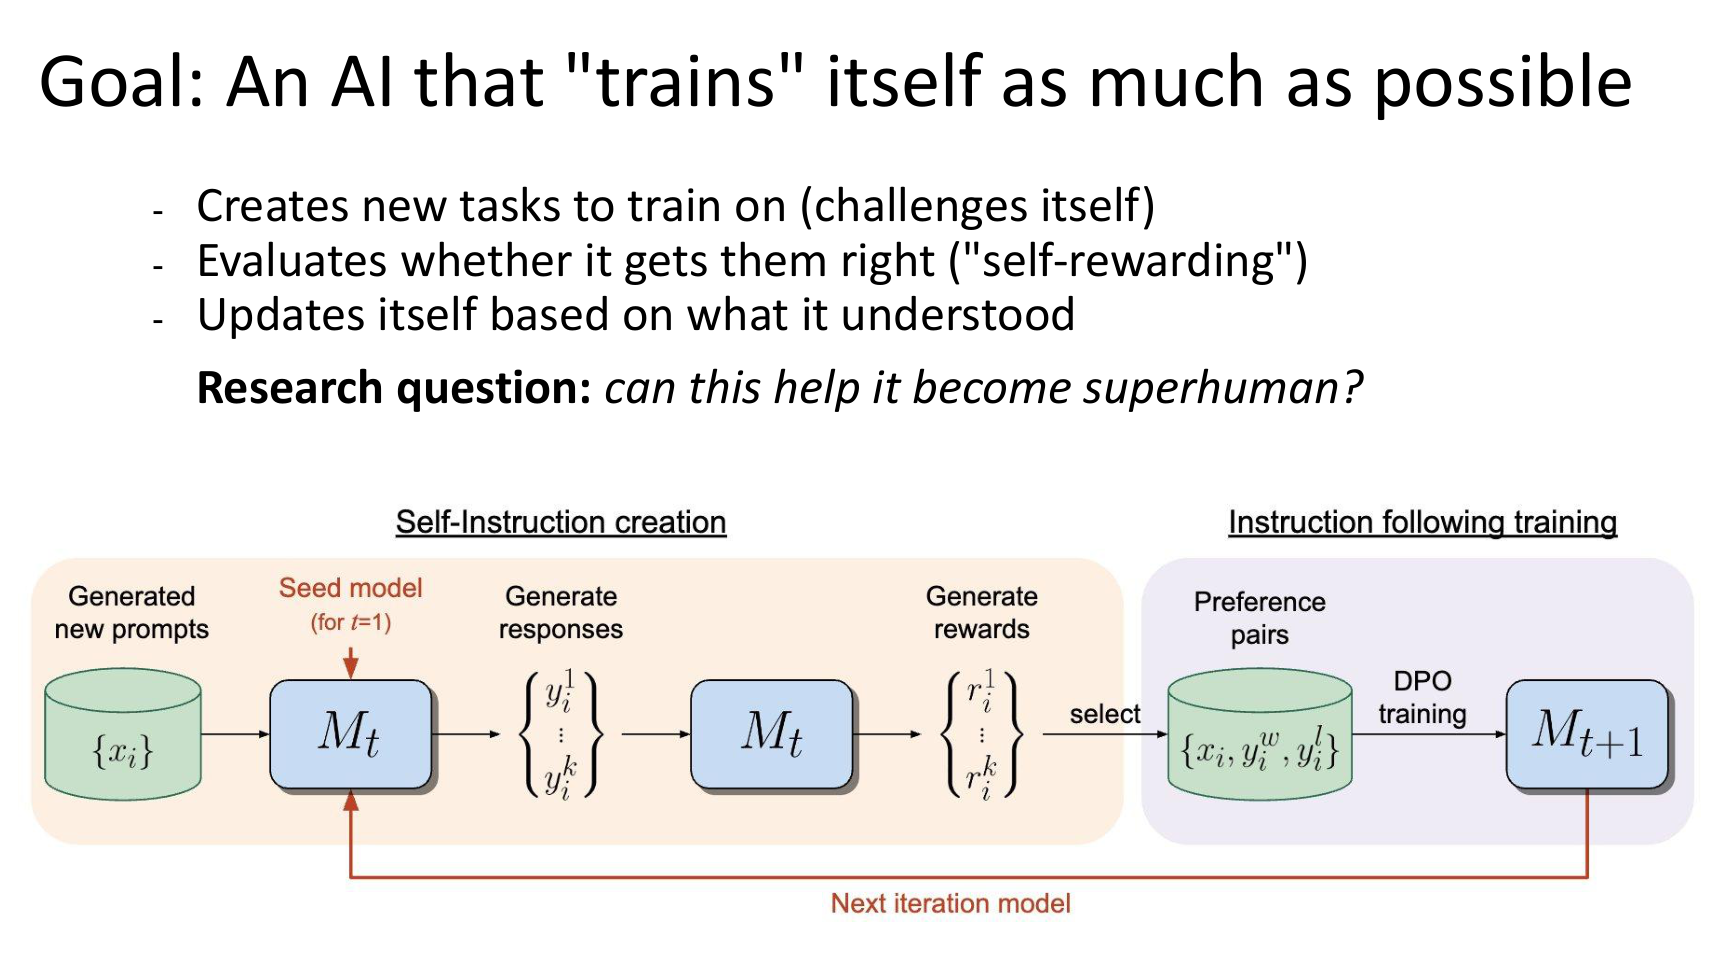
\includegraphics[width=0.82\textwidth]{../lectures/lec02_learning_to_reason/figures/lec02_fig_001.png}
\caption{Weston 对 self-training AI 的定义：能生成任务、分配 reward、并把这些 judgments 重新喂回训练流程。}
\end{figure}

这一定义已经隐含了本讲的中心思想。Reasoning 不仅是“生成更长的 chain-of-thought”，而是：\textbf{模型能否获得足够高质量的反馈信号，判断哪条思路更好、哪条思路只是看起来像思考。}

\subsection{System 1 失败为什么逼着我们走向 System 2}

在 Weston 的叙述里，当前 LLM 更像 \textbf{System 1}：反应快、擅长联想、每个 token 都是固定计算，但很容易学到不该学的相关性。幻觉、迎合用户错误观点、越狱，本质上都是“反应式模式匹配”超出安全工作区后的副产物。换句话说，问题不只是模型会错，而是它经常\textbf{没有显式的机制停下来检查自己。}

Weston 因此把 reasoning 引向了一个很务实的方向：与其要求模型凭空更聪明，不如先让它学会更系统地\textbf{验证（verification）、重写（rewriting）、分解（decomposition）和评价（judging）}。这就是他所说的 System 2 路线。

\subsection{后训练谱系：SFT、RLHF、DPO}

在进入 reasoning-specific 方法之前，讲者先回顾 pre-o1/r1 时代的 post-training 谱系：SFT 用任务示例继续做 next-token learning，RLHF 引入人类偏好与 reward model，而 DPO 则把 RLHF 的目标改写成一个更稳定直接的 preference optimization loss。

\begin{figure}[H]
\centering
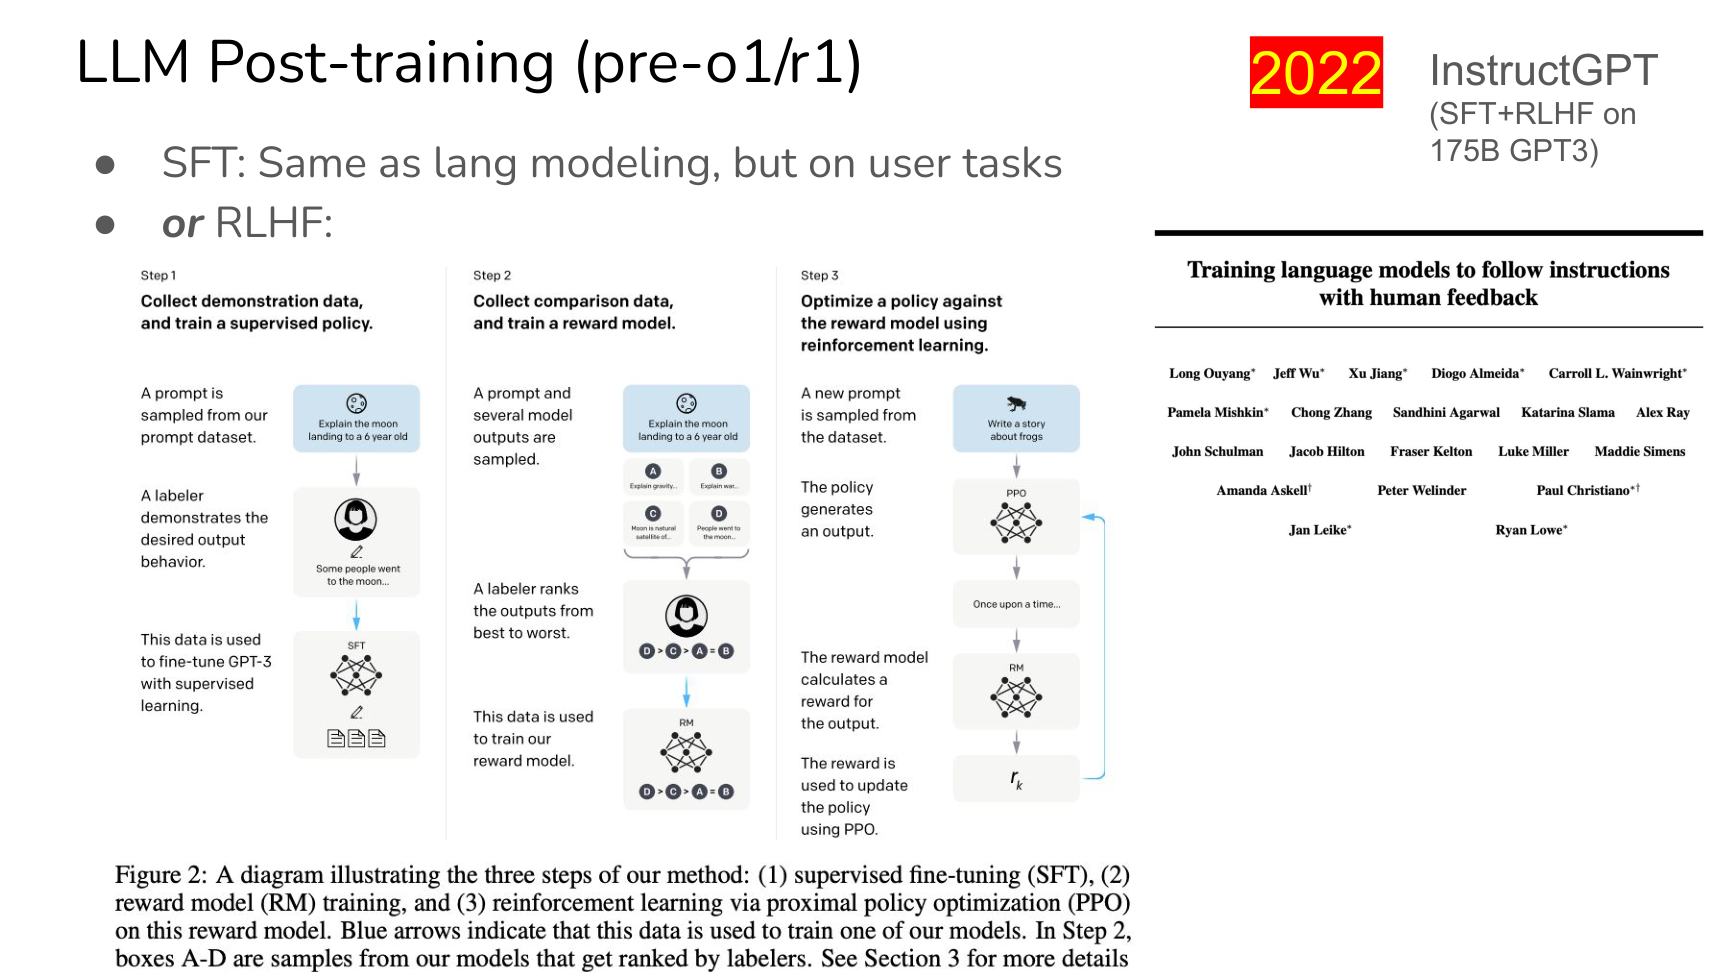
\includegraphics[width=0.80\textwidth]{../lectures/lec02_learning_to_reason/figures/lec02_fig_002.png}
\caption{SFT、RLHF、DPO 构成 Weston 后续所有训练 recipe 的基本骨架。}
\end{figure}

DPO 的标准写法是：
\[
\mathcal{L}_{\mathrm{DPO}}(\theta)=-\mathbb{E}_{(x,y_w,y_l)}\left[\log \sigma\left(\beta \log \frac{\pi_\theta(y_w \mid x)}{\pi_{\mathrm{ref}}(y_w \mid x)}-\beta \log \frac{\pi_\theta(y_l \mid x)}{\pi_{\mathrm{ref}}(y_l \mid x)}\right)\right]
\]
其中 $\pi_\theta$ 是要训练的模型，$\pi_{\mathrm{ref}}$ 是参考模型，$x$ 是输入指令，$y_w$ 与 $y_l$ 分别是胜出和败北回答，$\beta$ 控制偏离参考模型的强度。直觉上，DPO 不再单独训练一个 reward model 再跑 RL，而是直接把“更喜欢 $y_w$ 而不是 $y_l$”写进模型更新目标。

\begin{importantbox}{这条公式为什么重要}
Weston 之后讲的 self-rewarding、IRPO、meta-rewarding 都要回到同一个问题：\emph{偏好对从哪来？} DPO 本身不是答案，它只是一个非常好用的“执行器”。真正困难的是如何构造足够可信的 $(y_w, y_l)$。
\end{importantbox}

\section{主体讲解}

\subsection{先把验证这件事做清楚：CoVe、System 2 Attention、Branch-Solve-Merge}

\subsubsection{Chain-of-Verification：不是更长 CoT，而是更可审计的 CoT}

CoVe 的贡献在于，它把“再想一遍”拆成四个可解释的步骤：先给草稿答案，再生成 verification questions，然后独立回答这些问题，最后整合成最终答案。

\begin{figure}[H]
\centering
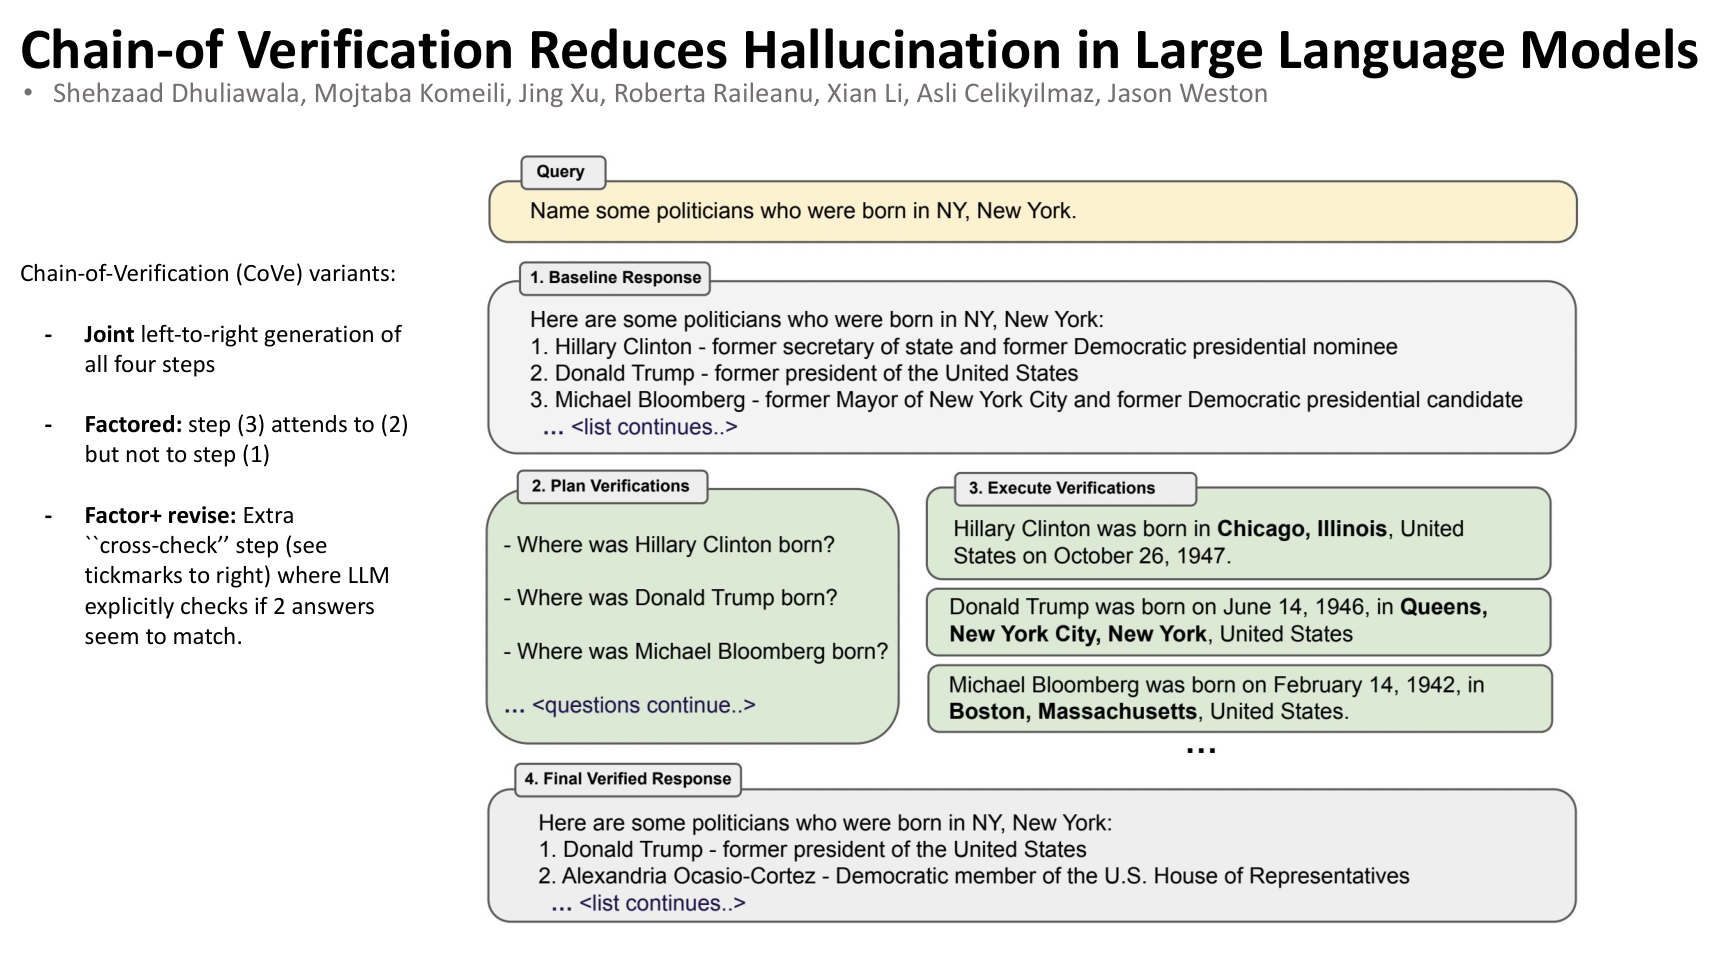
\includegraphics[width=0.78\textwidth]{../lectures/lec02_learning_to_reason/figures/lec02_fig_003.png}
\caption{CoVe 把验证流程显式拆解，核心目的是减少最终回答对原始错误草稿的路径依赖。}
\end{figure}

\begin{lstlisting}
Draft an initial answer
Plan verification questions
Answer each verification question independently
Synthesize a final verified response
\end{lstlisting}

这和第一讲里那种“让模型多采样几条 CoT 再投票”不同。CoVe 面向的是 factuality / hallucination 场景：如果错误来自事实断言，而不是搜索宽度不足，那么更关键的是\textbf{把事实核查环节显式写进流程}。

\paragraph{为什么要独立回答 verification questions}
如果 verification step 继续强依赖原始草稿，那么模型只是在原错误附近做润色。CoVe 要求各验证问题独立作答，目的正是防止 answer contamination。

\subsubsection{System 2 Attention 与 Branch-Solve-Merge}

Weston 随后给出另外两类 System 2 方法。System 2 Attention（S2A）不急着回答，而是先重写问题，尽量移除与任务无关的偏见和干扰项，再基于重写后的问题作答。

\begin{figure}[H]
\centering
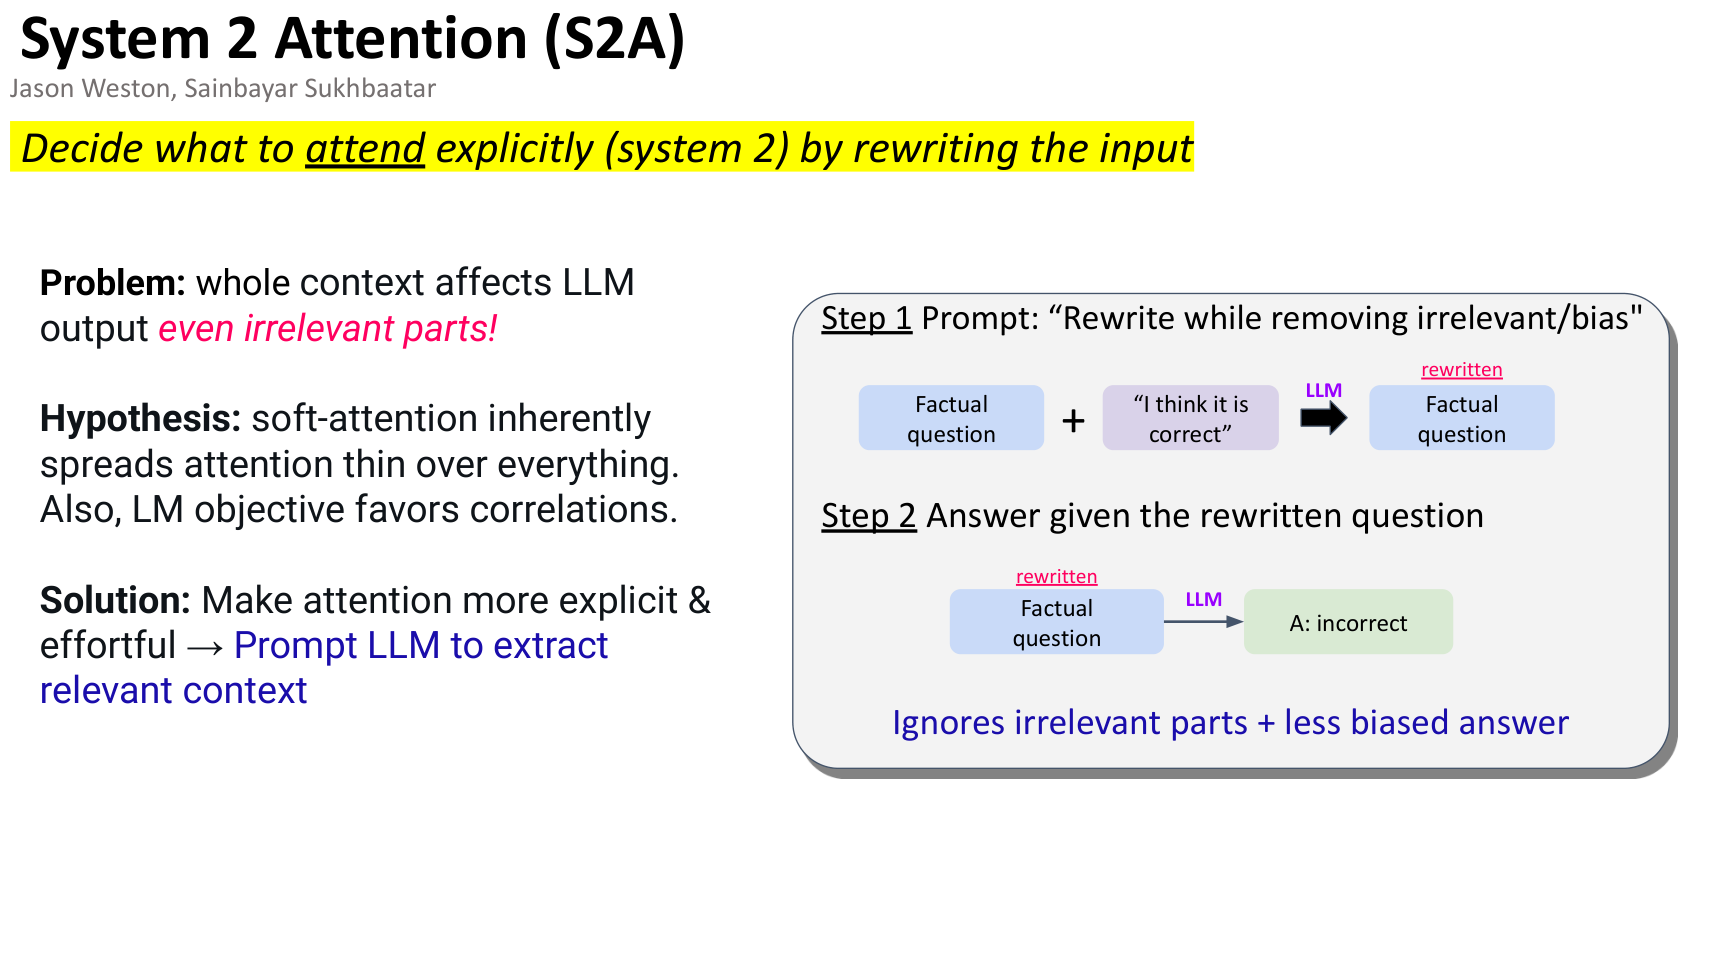
\includegraphics[width=0.80\textwidth]{../lectures/lec02_learning_to_reason/figures/lec02_fig_004.png}
\caption{S2A 的关键是先决定“应该注意什么”，而不是直接在有偏输入上给答案。}
\end{figure}

这背后的直觉非常实用：不少 hallucination 不是知识完全缺失，而是模型注意力被噪声、用户偏见或表述方式带偏了。S2A 先做 \textbf{attention selection}，再做 answering。

Branch-Solve-Merge 则把复杂评价或生成任务拆成多个子问题，分别求解后再融合。它更像“评估任务也需要 planning”。和第一讲的 Tree of Thoughts 很像，只是这里的对象更多是\textbf{response evaluation} 而不是 search over candidate answers。

\begin{knowledgebox}{本节的统一主线}
Weston 给出的 System 2 方法有一个共同点：它们都把“多花一点 token”变成了“对哪一步花 token、为什么花 token”的结构化决策。
\end{knowledgebox}

\subsection{Self-Rewarding：为什么 reasoning learning 会卡在 human bottleneck}

\subsubsection{标准 RLHF 的扩展瓶颈}

当模型还不强时，人类给偏好标签并不太困难；一旦回答很长、主题专业、甚至模型在某些方面超过普通评审，人类就会越来越难稳定判断“哪个更好”。

\begin{figure}[H]
\centering
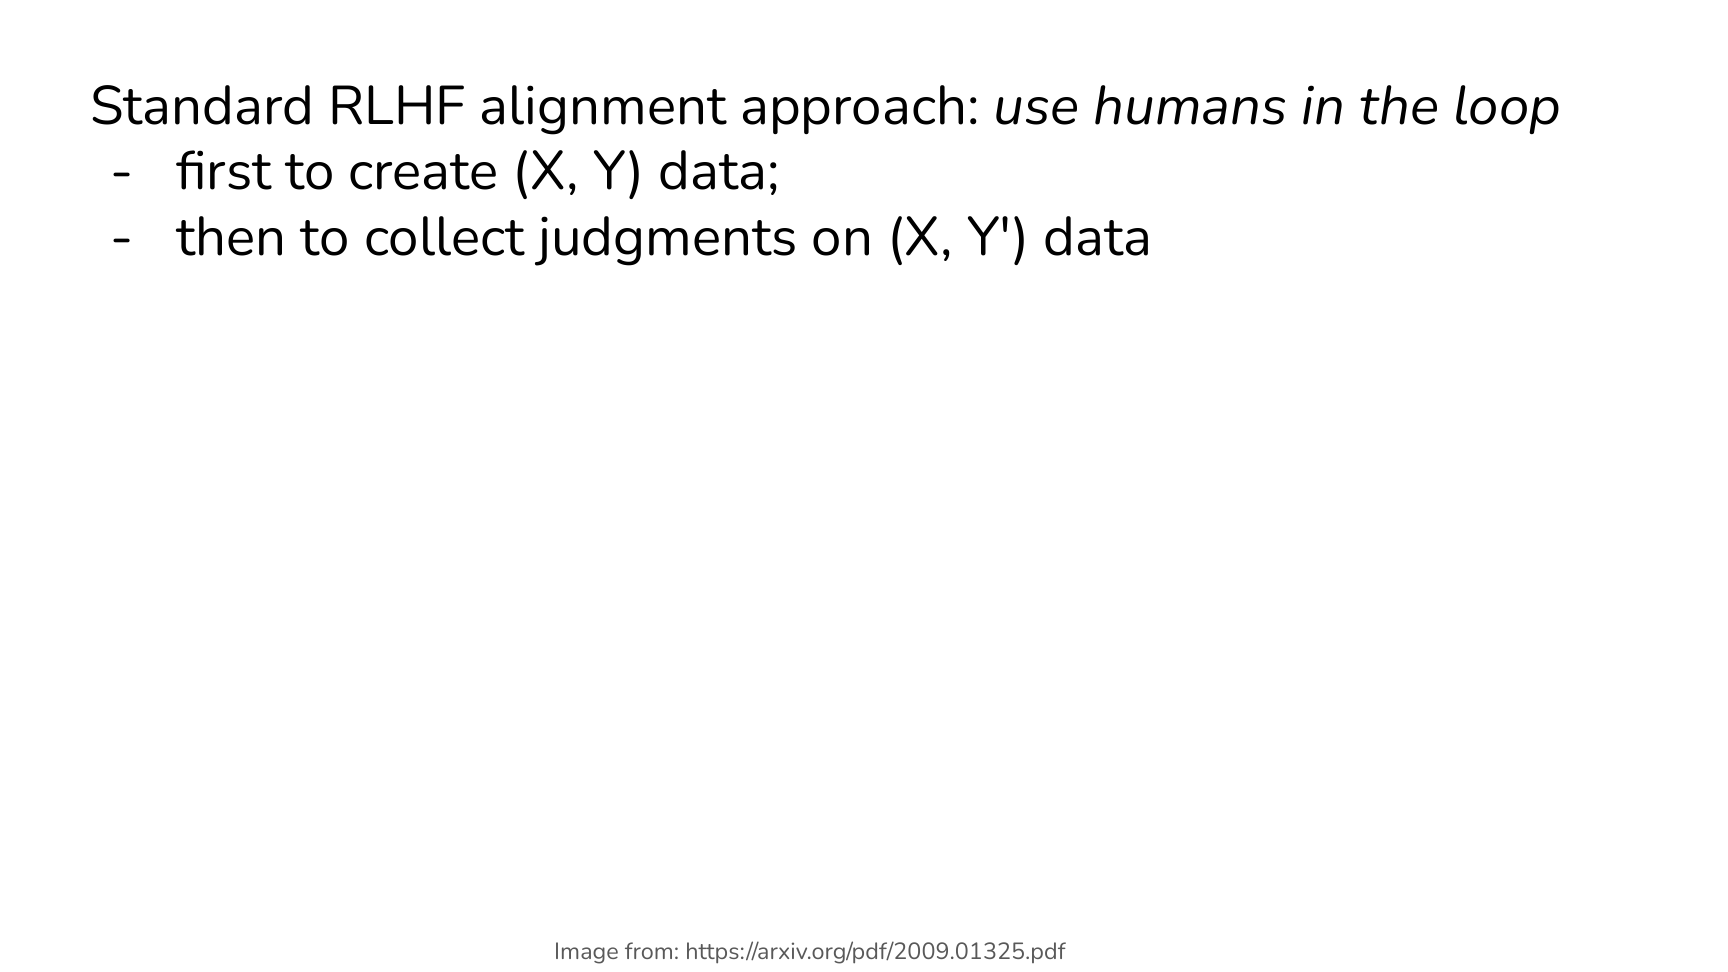
\includegraphics[width=0.74\textwidth]{../lectures/lec02_learning_to_reason/figures/lec02_fig_005.png}
\caption{标准 RLHF 把人类放在数据生产和偏好判断两个关键位置，因此扩展能力直接受限于人类评审吞吐量。}
\end{figure}

Weston 的研究问题很明确：\textbf{如果继续提升模型需要更高质量的 judgments，而 humans in the loop 已经成为瓶颈，那么能不能让模型学习生成这些 judgments？}

\subsubsection{Self-Rewarding LM：actor 和 judge 双能力模型}

Self-rewarding LM 的定义不是“模型给自己打分”这么简单。Weston 强调它至少要有两种能力：
\begin{itemize}
\item \textbf{instruction following capability}：能对用户指令给出较好回答。
\item \textbf{evaluation capability}：能区分更好和更差的回答，并给出可用的偏好信号。
\end{itemize}

\begin{figure}[H]
\centering
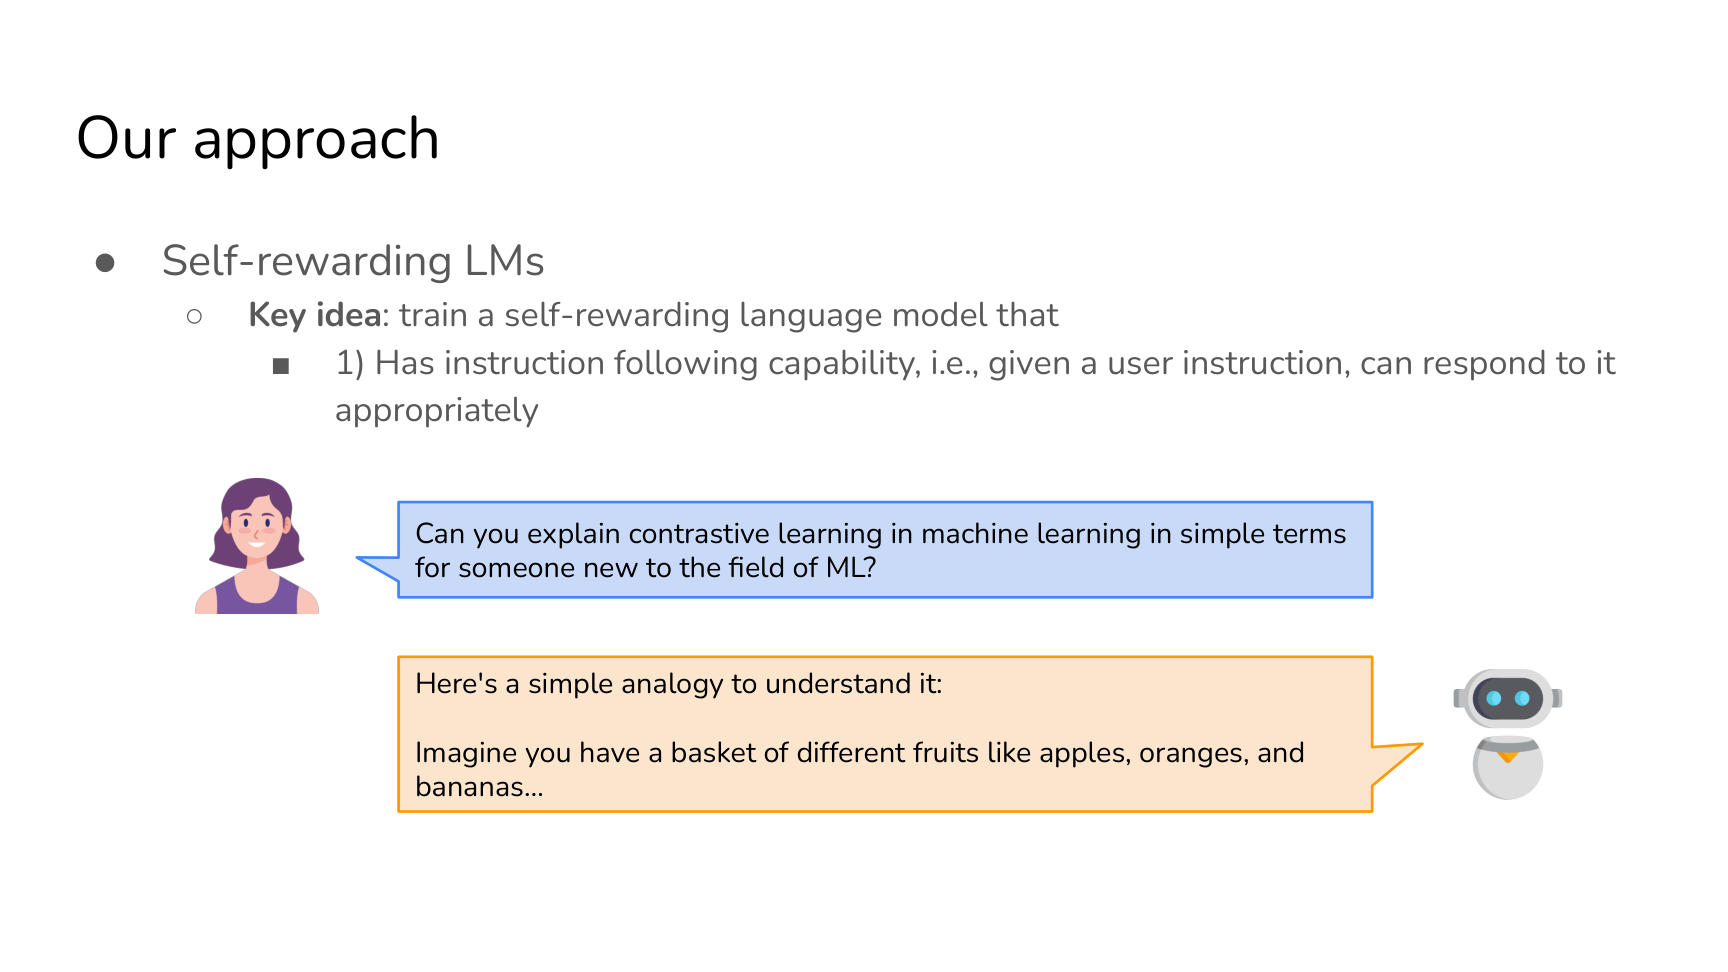
\includegraphics[width=0.76\textwidth]{../lectures/lec02_learning_to_reason/figures/lec02_fig_006.png}
\caption{Self-rewarding 模型既是 actor 也是 judge。Weston 的关键不是“省人力”，而是让 evaluator 能随着 actor 一起成长。}
\end{figure}

可以用一个极简抽象写成：
\[
\mathcal{D}_{t+1}=\mathcal{D}_{t}\cup\{(x,\{(y_i,r_i)\}_{i=1}^{k})\}
\]
其中 $\mathcal{D}_t$ 是已有数据集，模型对同一指令 $x$ 生成多个回答 $y_i$ 并赋予分数 $r_i$，然后把这些 judged candidates 再变成新的训练材料。

\paragraph{为什么这不是自嗨}
如果模型只会生成、不会评估，那么新的训练数据不过是旧偏差的放大器。Self-rewarding 的真正难点在于 judge 能否提供\textbf{比现有 actor 更可靠的排序}。

\subsubsection{训练 recipe 与实验设计}

Lecture 给出的 recipe 很具体：从一个带少量 seed instruction-following data 和 evaluation data 的模型出发，在每轮中生成 prompts、candidate responses 和 self-rewards，然后把选出的 preference pairs 用 DPO 继续训练。

\begin{figure}[H]
\centering
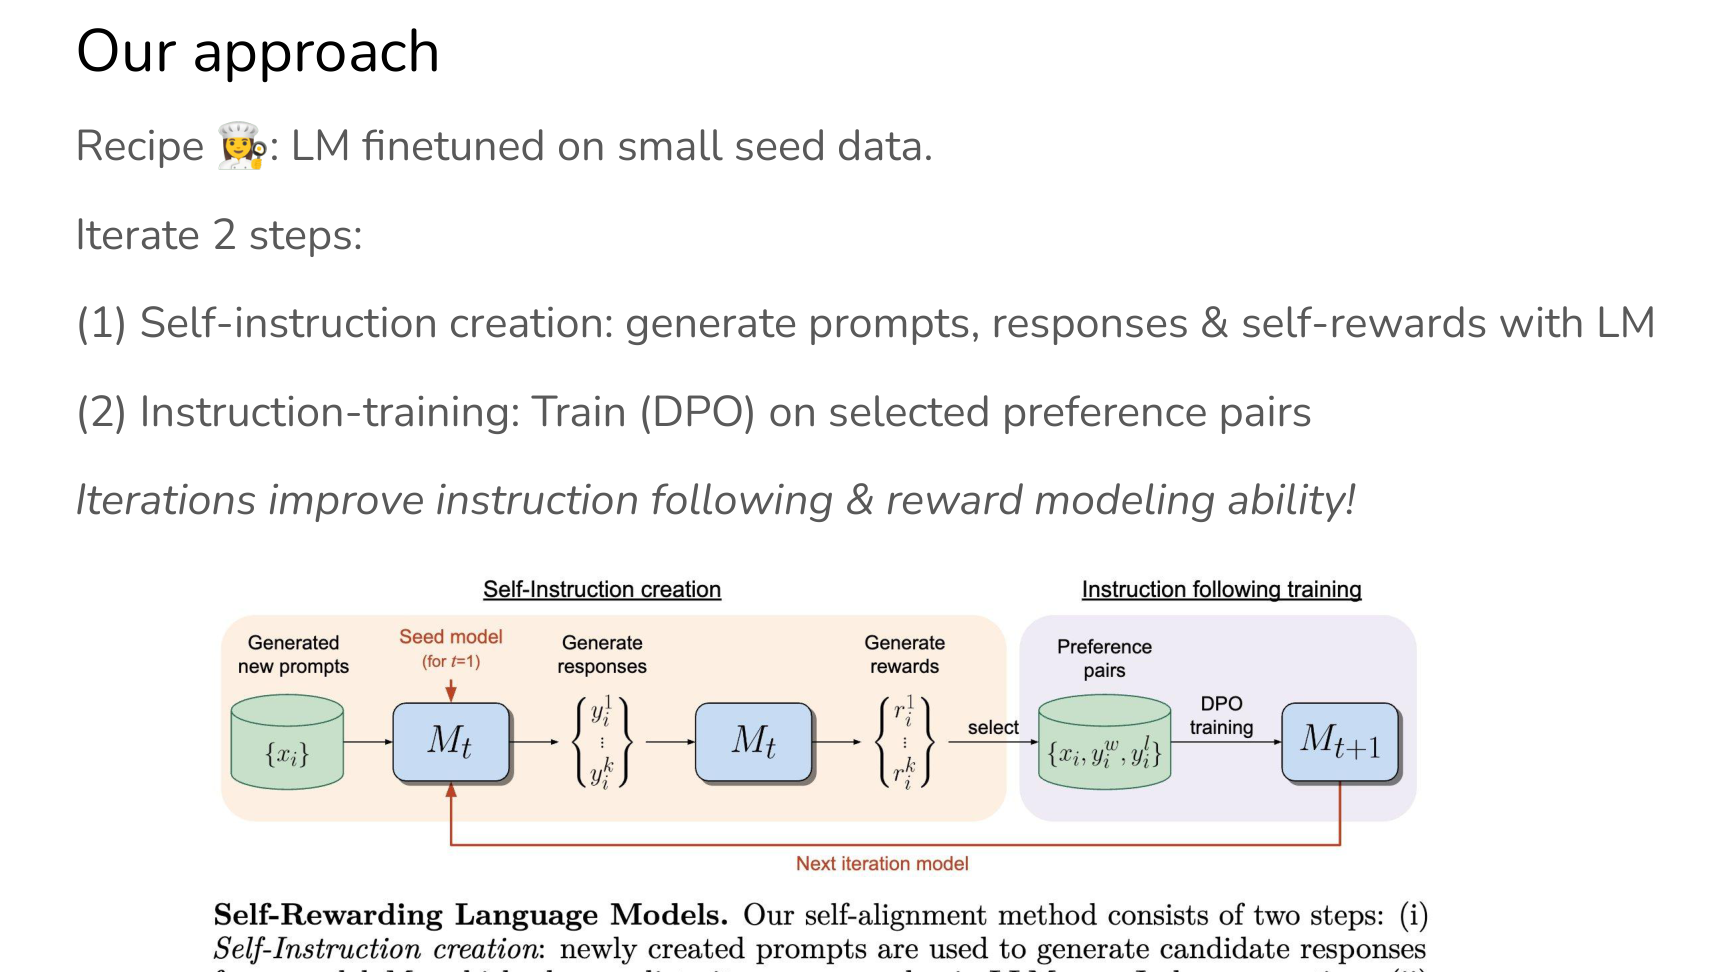
\includegraphics[width=0.78\textwidth]{../lectures/lec02_learning_to_reason/figures/lec02_fig_007.png}
\caption{Self-rewarding 训练 recipe：生成、判断、筛选、DPO，再迭代。}
\end{figure}

\begin{lstlisting}
Initialize M1 with seed instruction-following and evaluation data
For each iteration t:
    generate prompts, candidate responses, and self-rewards with Mt
    select preference pairs from the judged candidates
    run DPO to obtain M(t+1)
\end{lstlisting}

讲者特别展示了 LLM-as-a-Judge prompt 的维度设计：relevance、coverage、usefulness、clarity、expertise。这个细节非常关键，因为 reasoning training 不是只要一个 scalar reward 就够了；如果 reward 的来源不可解释、不可审计，那么后续迭代只会更脆弱。

\begin{figure}[H]
\centering
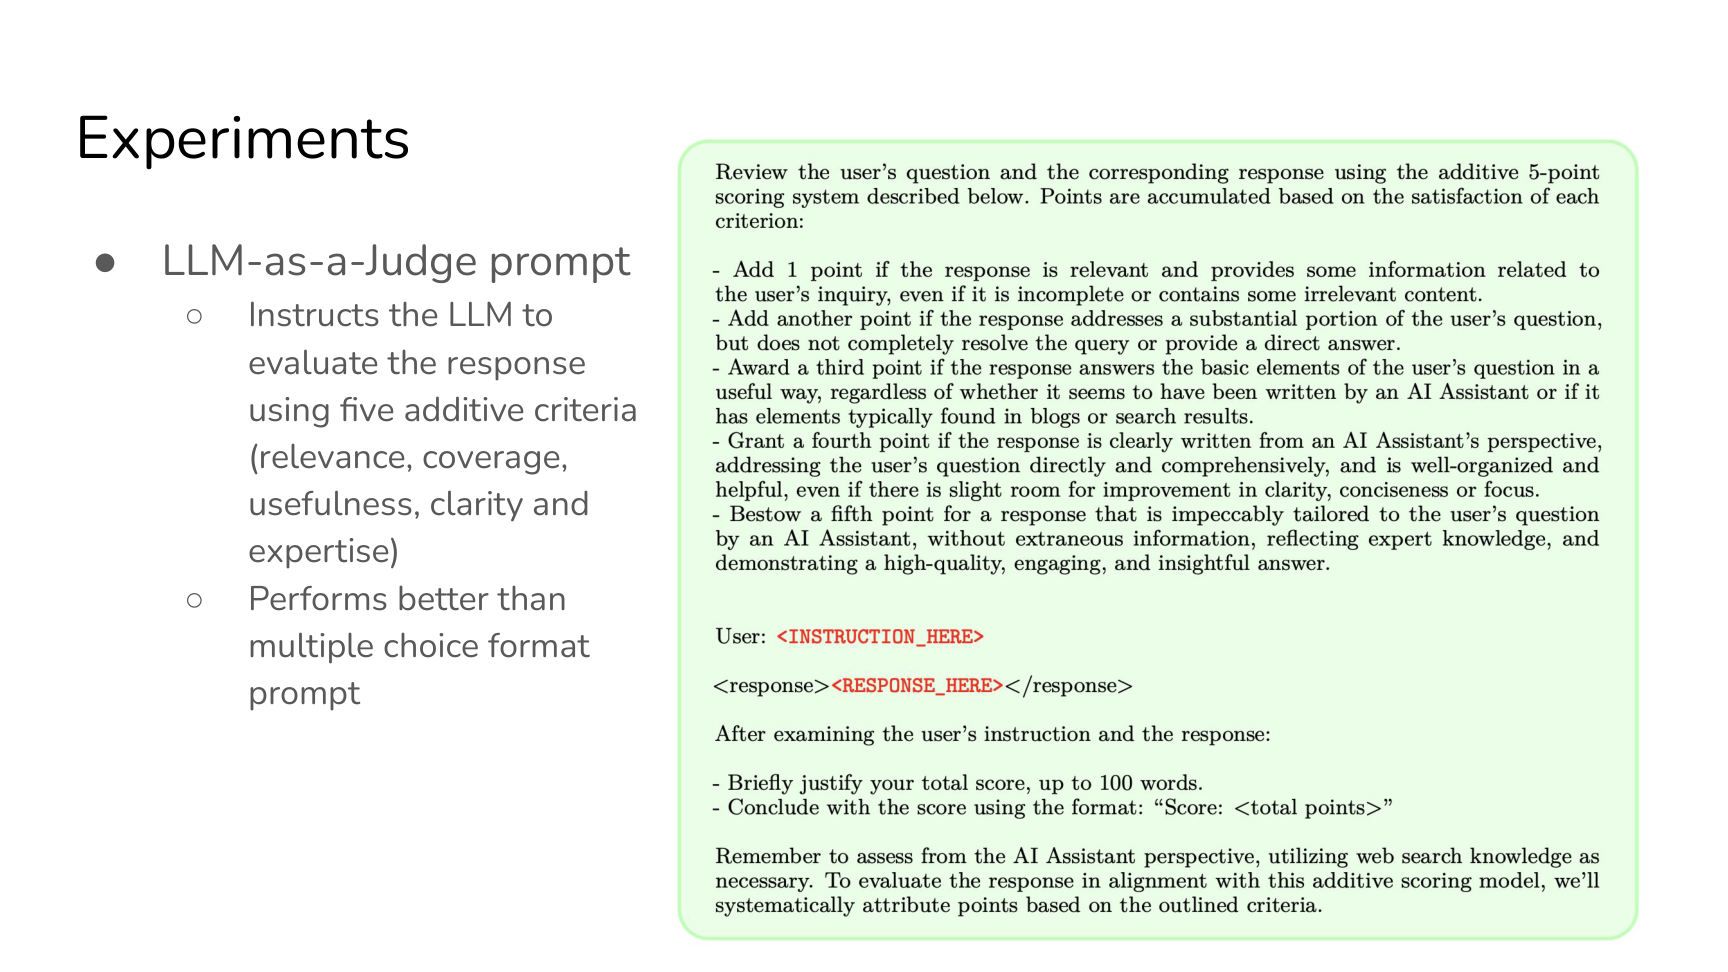
\includegraphics[width=0.78\textwidth]{../lectures/lec02_learning_to_reason/figures/lec02_fig_008.png}
\caption{Weston 强调 judge prompt 要拆解成多个 criteria，避免 evaluator 只学到模糊的“我喜欢这个回答”。}
\end{figure}

\paragraph{实验结果的真正含义}
Self-rewarding 模型在 instruction following 和 reward modeling 两个轴上都持续提升，这说明“学会 judging”不会天然拖累“学会 acting”。但讲者没有把这个结果夸成万能方案，因为 reasoning tasks 仍然比一般 instruction following 更难，需要更强的可验证信号。

\subsection{IRPO：把 preference optimization 从 style alignment 拉回 reasoning}

\subsubsection{为什么 reasoning 需要更强的 reward structure}

Weston 在第一个 self-rewarding 结果之后立刻承认一个限制：模型确实更会回答、也更会评分了，但\textbf{reasoning task 仍然提升有限。} 原因是通用偏好标签更像 style / helpfulness alignment，而 reasoning task 需要对中间思路的成败有更细粒度的 credit assignment。

\begin{figure}[H]
\centering
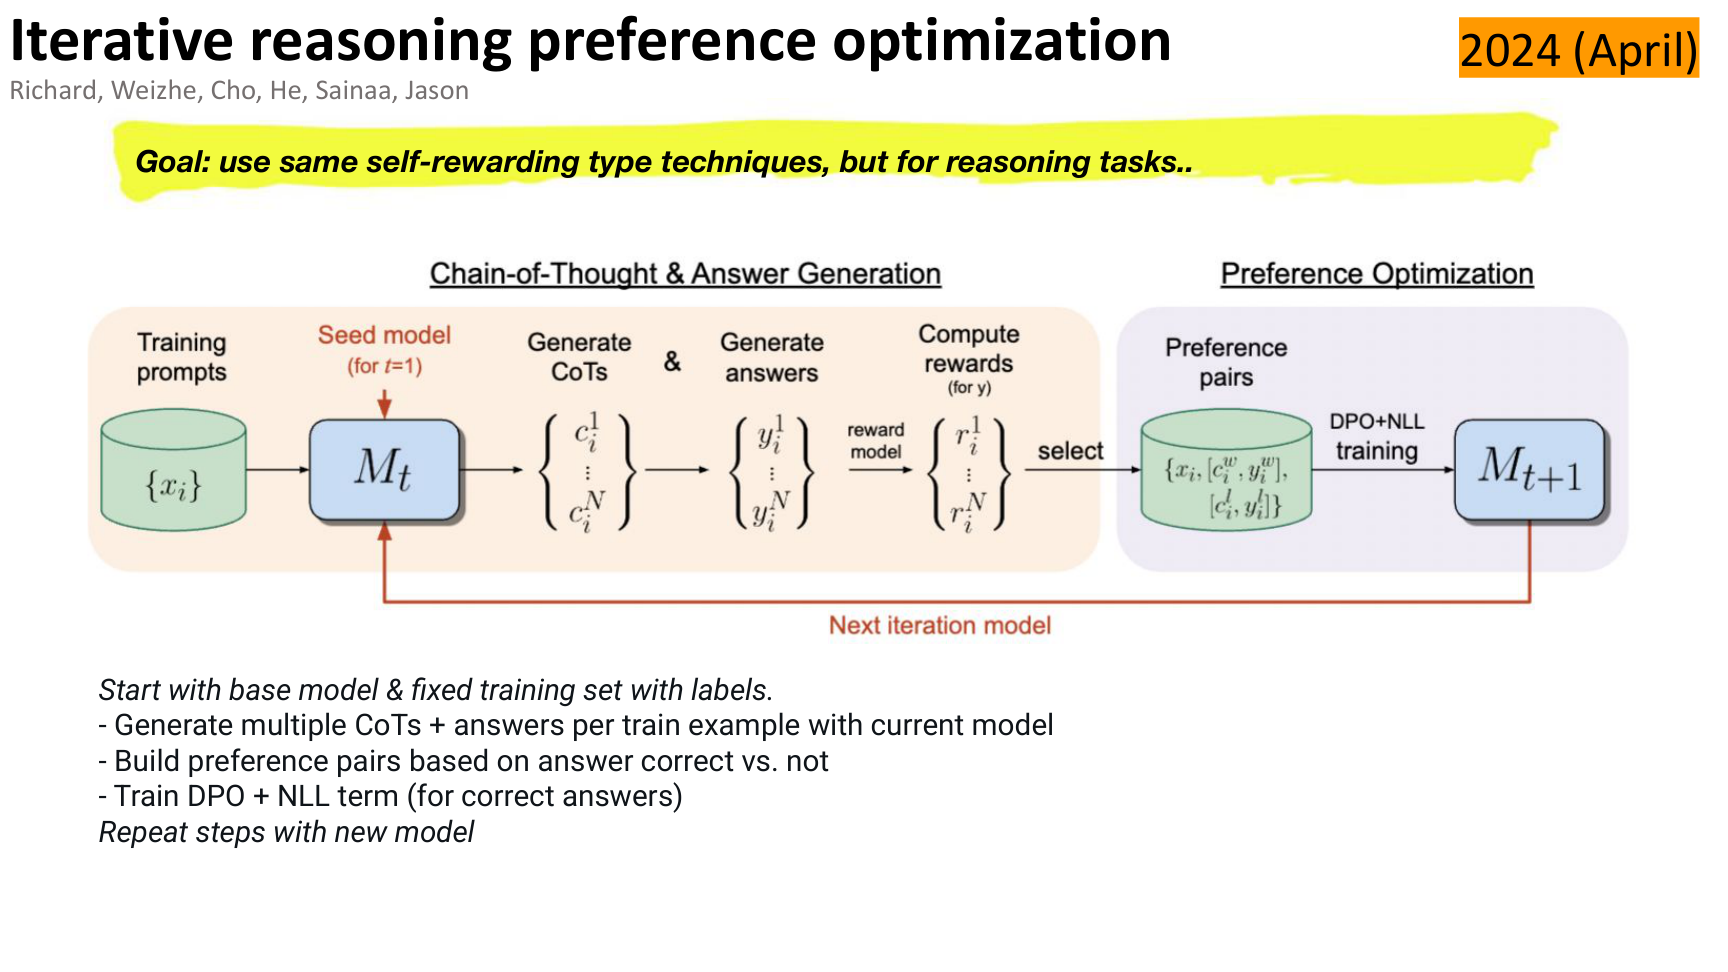
\includegraphics[width=0.78\textwidth]{../lectures/lec02_learning_to_reason/figures/lec02_fig_009.png}
\caption{IRPO 的出发点：reasoning task 需要的不只是好回答，而是“哪条思路最终导致了可验证正确答案”。}
\end{figure}

IRPO 的基本流程是：对每个问题采样多条 chain-of-thought，抽取最终答案，用可验证规则判断最终答案是否正确，再保留那些通向正确 final answer 的 reasoning traces，把它们与失败 traces 组成 preference pairs。

它的目标写成：
\[
\mathcal{L}_{\mathrm{IRPO}}=\mathcal{L}_{\mathrm{DPO}}+\lambda\,\mathcal{L}_{\mathrm{NLL}}(y^{\star}_{\mathrm{cot}})
\]
其中 $\mathcal{L}_{\mathrm{DPO}}$ 负责学习 winning / losing CoT 的相对偏好，$\mathcal{L}_{\mathrm{NLL}}$ 则继续鼓励模型模仿正确 reasoning trace，$y^{\star}_{\mathrm{cot}}$ 表示到达可验证正确 final answer 的那条 CoT。

\begin{lstlisting}
Sample multiple CoT candidates per problem
Extract the final answer from each candidate
Keep trajectories whose final answer is verifiably correct
Create winning/losing reasoning pairs
Train with DPO plus an NLL term on the winning traces
\end{lstlisting}

\paragraph{为什么 negative examples 是关键}
Lecture 明确指出：如果只做 SFT，chosen 和 rejected generations 在 token 级概率上常常被拉得太近，模型无法真正学会“哪种 reasoning style 会通往正确答案”。IRPO 需要明确失败样本，才能把 reasoning 区分开来。

\subsubsection{IRPO 的边界条件}

IRPO 最大的优点是 reward 来自\textbf{可验证 final answer}，这让 reasoning learning 有了更坚实的地基。但它也有明确边界：
\begin{itemize}
\item 任务必须存在可验证答案，至少 final answer 要能自动判对错。
\item 对开放式任务、创造性任务、模糊评价任务，IRPO 的 reward grounding 会变弱。
\item 它仍然是在固定问题集上循环，不等于 agent 已经能在开放环境中自发发现新 reasoning tasks。
\end{itemize}

\subsection{Thinking LLMs、Meta-Rewarding 与 EvalPlanner}

\subsubsection{Thinking LLMs：thought generation 不应只服务数学}

Weston 进一步指出，o1 / R1 式“先想后答”不应该只限于数学或可验证推理。Thinking LLMs / Thought Preference Optimization（TPO）的目标，是让模型在一般 instruction following 任务里也学会 thought generation。

\begin{figure}[H]
\centering
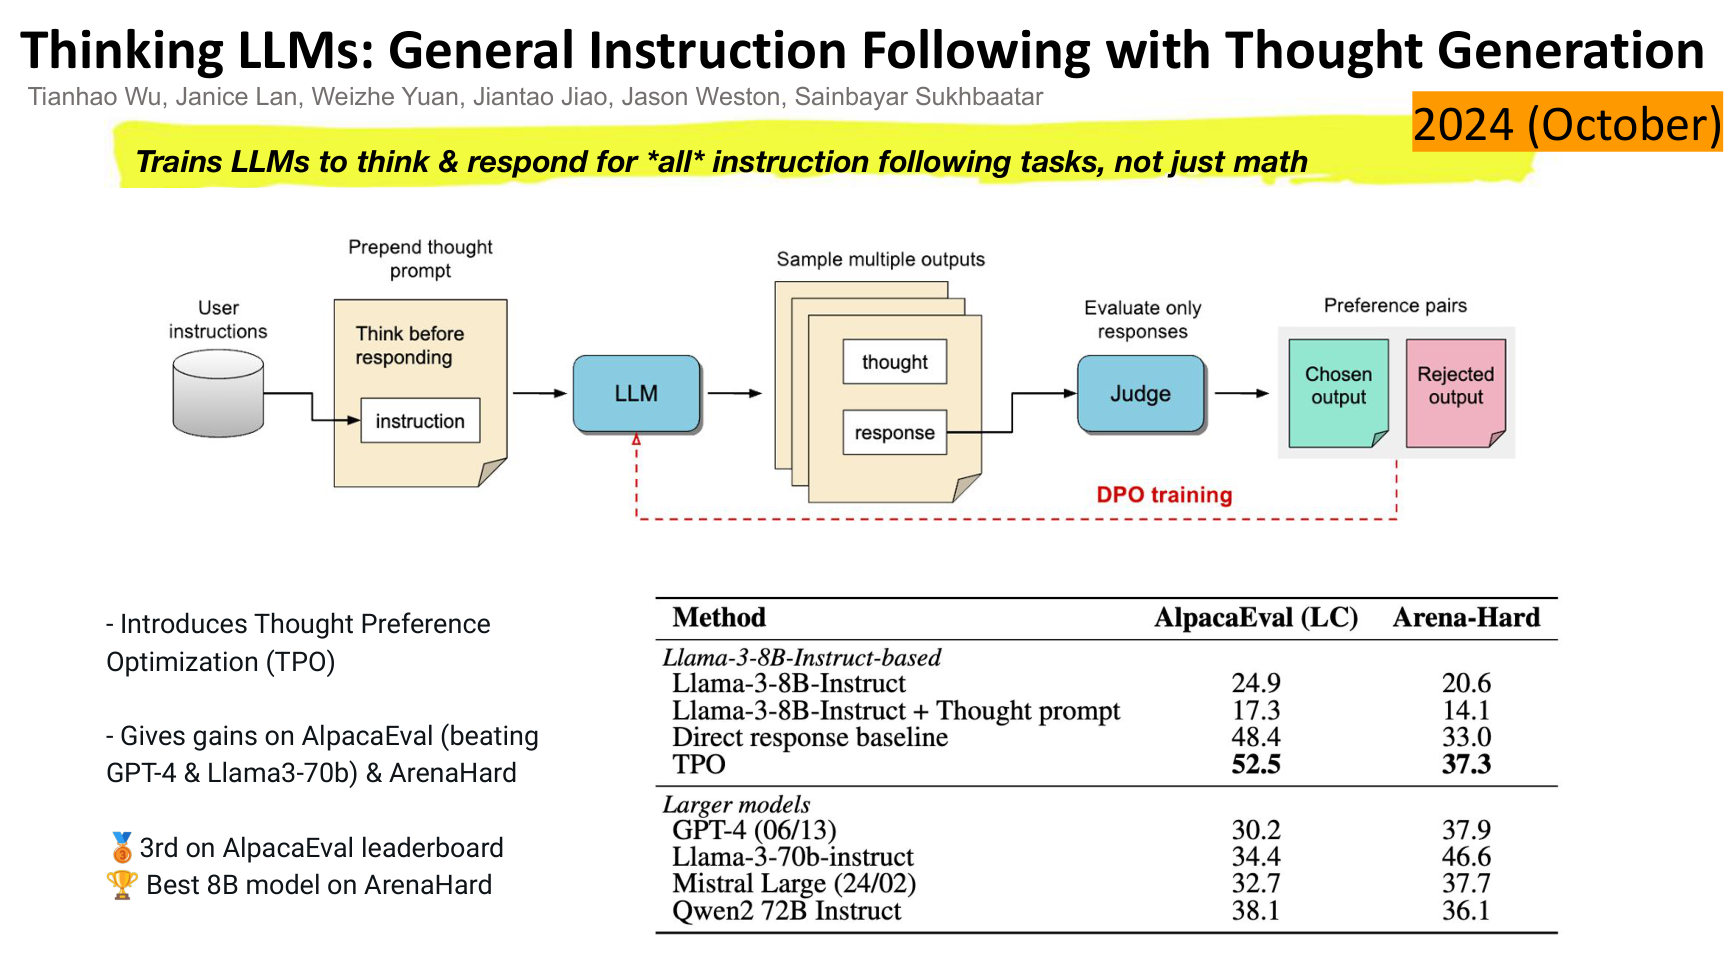
\includegraphics[width=0.76\textwidth]{../lectures/lec02_learning_to_reason/figures/lec02_fig_010.png}
\caption{Thinking LLMs 的主张：thought generation 应该成为更广泛 instruction following 的默认能力，而不是 reasoning benchmark 的特例。}
\end{figure}

这里的关键不是“每道题都写一长串想法”，而是让模型学会何时需要显式计划、何时只需快速回答。对 agent 来说，这意味着 reasoning policy 也应该被训练，而不仅是 final answer style。

\subsubsection{Meta-Rewarding：judge 也要继续被训练}

如果 self-rewarding 把 actor 和 judge 放进同一个模型，下一步自然是：\textbf{judge 本身怎么变强？} Meta-Rewarding 的回答是，让模型不仅学习回答，还学习对 judgment 进行 meta-judgment。

\begin{figure}[H]
\centering
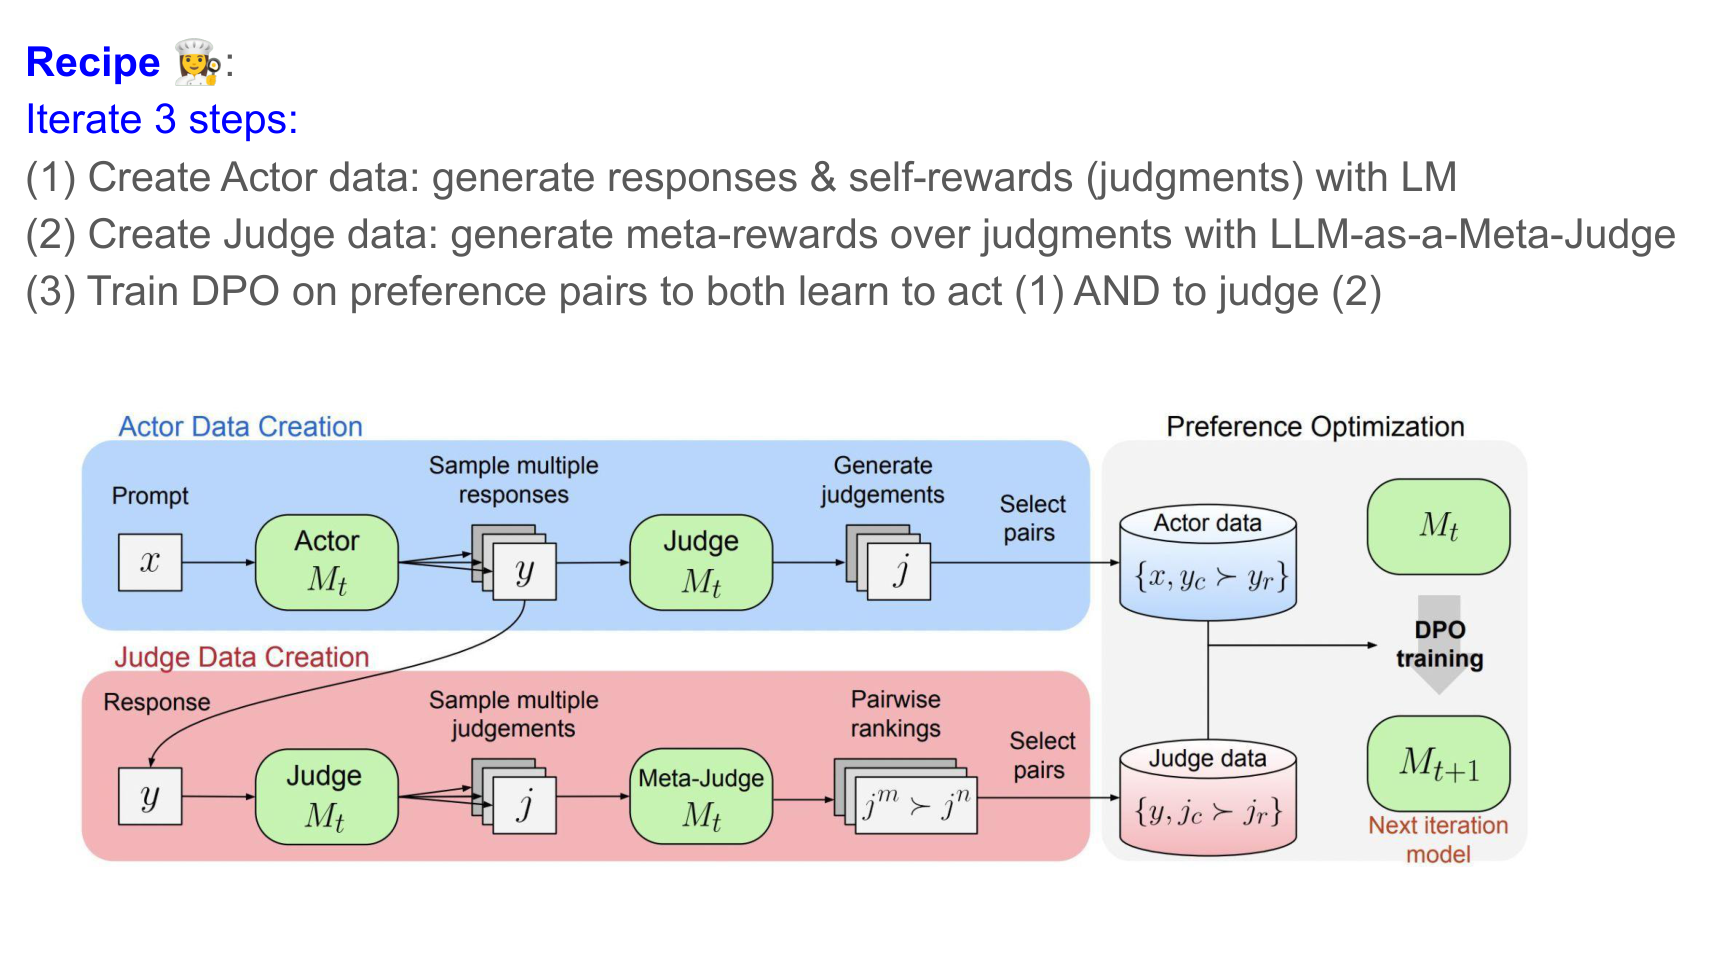
\includegraphics[width=0.78\textwidth]{../lectures/lec02_learning_to_reason/figures/lec02_fig_011.png}
\caption{Meta-Rewarding 的三步循环：生成 actor data、生成 judge data、同时训练 actor 与 judge。}
\end{figure}

一个简化的写法是：
\[
p(i \succ j)=\sigma(s_i-s_j)
\]
其中 $s_i$ 和 $s_j$ 是两个 judgments 的 latent score，$\sigma$ 把分差转成偏好概率。Lecture 用 Elo-style intuition 说明：如果能比较 judgment 本身谁更好，我们就能反过来训练更强的 judge。

\begin{lstlisting}
Create actor data: responses plus self-judgments
Create judge data: meta-judge comparisons over those judgments
Train DPO objectives for both the actor and the judge
\end{lstlisting}

Meta-Rewarding 的价值在于，它直面了“judge 会不会比 actor 落后”的问题。许多系统失败，不是因为生成器不会说，而是因为筛选器不会选。Weston 的路线是把筛选器也当成要持续学习的对象。

\subsubsection{EvalPlanner：让 judge 先计划再打分}

最后，EvalPlanner 把同样的想法推到 evaluation task 上：若评估本身也很难，那么 judge 也应该有自己的 chain-of-thought、planning 和可验证训练数据。

\begin{figure}[H]
\centering
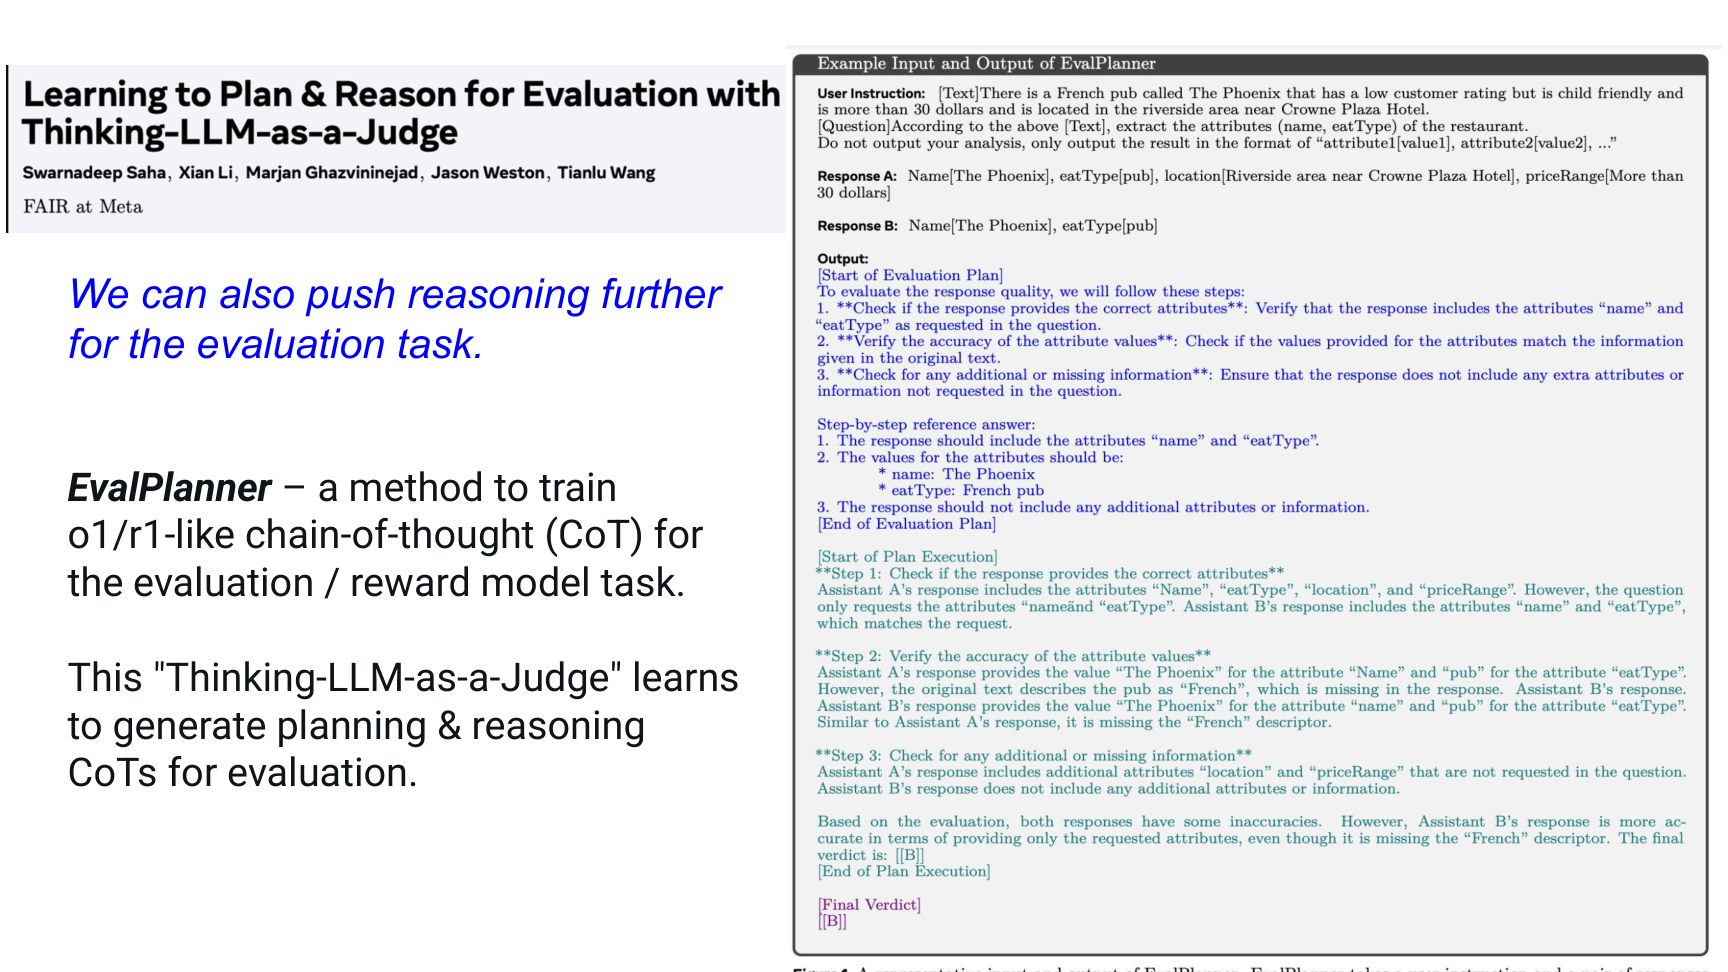
\includegraphics[width=0.78\textwidth]{../lectures/lec02_learning_to_reason/figures/lec02_fig_012.png}
\caption{EvalPlanner 把 evaluation task 转成可验证推理任务，训练的是“会规划的 judge”。}
\end{figure}

\begin{lstlisting}
Generate a good response y to prompt x
Perturb x into a similar prompt x' and generate y'
Convert the pair into a verifiable evaluation task
Train a thinking judge to plan before scoring
\end{lstlisting}

这一步非常关键。到这里，本讲已经把 reasoning learning 的难点重新表述为：\textbf{谁来给出足够好的 reward / judgment，以及这个 reward model 自身如何学习。}

\section{关键公式、算法与 readings 的连接}

\subsection{DPO：本讲所有 recipe 的优化执行器}

DPO reading 之所以重要，不是因为它单独就解决了 reasoning，而是因为它把“有偏好对就能训练”的这件事做得足够简单稳定。Weston 的系统几乎都默认用 DPO 或其变体做最后的优化，因此如果读者忽略 DPO，就会误以为这些方法的创新在于 loss 本身；实际上，创新更常在于\textbf{偏好对是如何被构造出来的。}

\subsection{IRPO：从 response preference 走向 reasoning preference}

IRPO reading 正好补上了 lecture 的核心转折。它证明 reasoning task 上最大的痛点不是“没有 preference optimization”，而是“没有 reasoning-aware preference pairs”。一旦 final answer 可验证，就可以把 CoT 也纳入 preference learning。

\subsection{CoVe：验证先于自信}

CoVe reading 在本讲里承担的是“方法论校正”的角色。它提醒我们，面对 hallucination 问题时，最重要的未必是生成更多候选，而是把 verification workflow 明确写出来，让模型先问“我该如何检查自己”。

\section{失败模式、边界条件与前后讲联系}

\subsection{本讲最重要的失败模式}

\begin{enumerate}
\item \textbf{把 self-rewarding 理解成“模型随便给自己打分”。} 没有可解释 criteria 和种子 judge 数据时，这会迅速漂移。
\item \textbf{把 DPO 当成 reasoning 的全部。} DPO 只是优化器；如果 winning/losing pairs 不携带真实 reasoning signal，它只会学到风格偏好。
\item \textbf{把 CoVe、S2A 当成更长 CoT。} 这些方法真正关心的是验证结构，而不是 token 数。
\item \textbf{在没有可验证 final answer 的任务上直接照搬 IRPO。} 一旦 reward grounding 变弱，reasoning preference 就会变得不可靠。
\item \textbf{忽略 judge 的学习问题。} 很多 agent pipeline 只训练 actor，却让 evaluator 原地踏步，这会导致系统上限卡死。
\end{enumerate}

\subsection{与前后讲的联系}

第一讲讨论的是 inference-time compute 的分配：如何在推理时生成、筛选、修正 reasoning traces。本讲则把焦点移到 training time：如何\textbf{让模型在训练中习得这些 reasoning / judging 行为。} 下一讲 Yu Su 会进一步把 reasoning 放进 language agent 框架，讨论 memory、planning、world model 等结构能力。这意味着课程主线正在从“如何让单个模型更会想”扩展到“如何让 agent 系统在外部环境中更会记、更会规划、更会行动”。

\section{本章小结}

\begin{figure}[H]
\centering
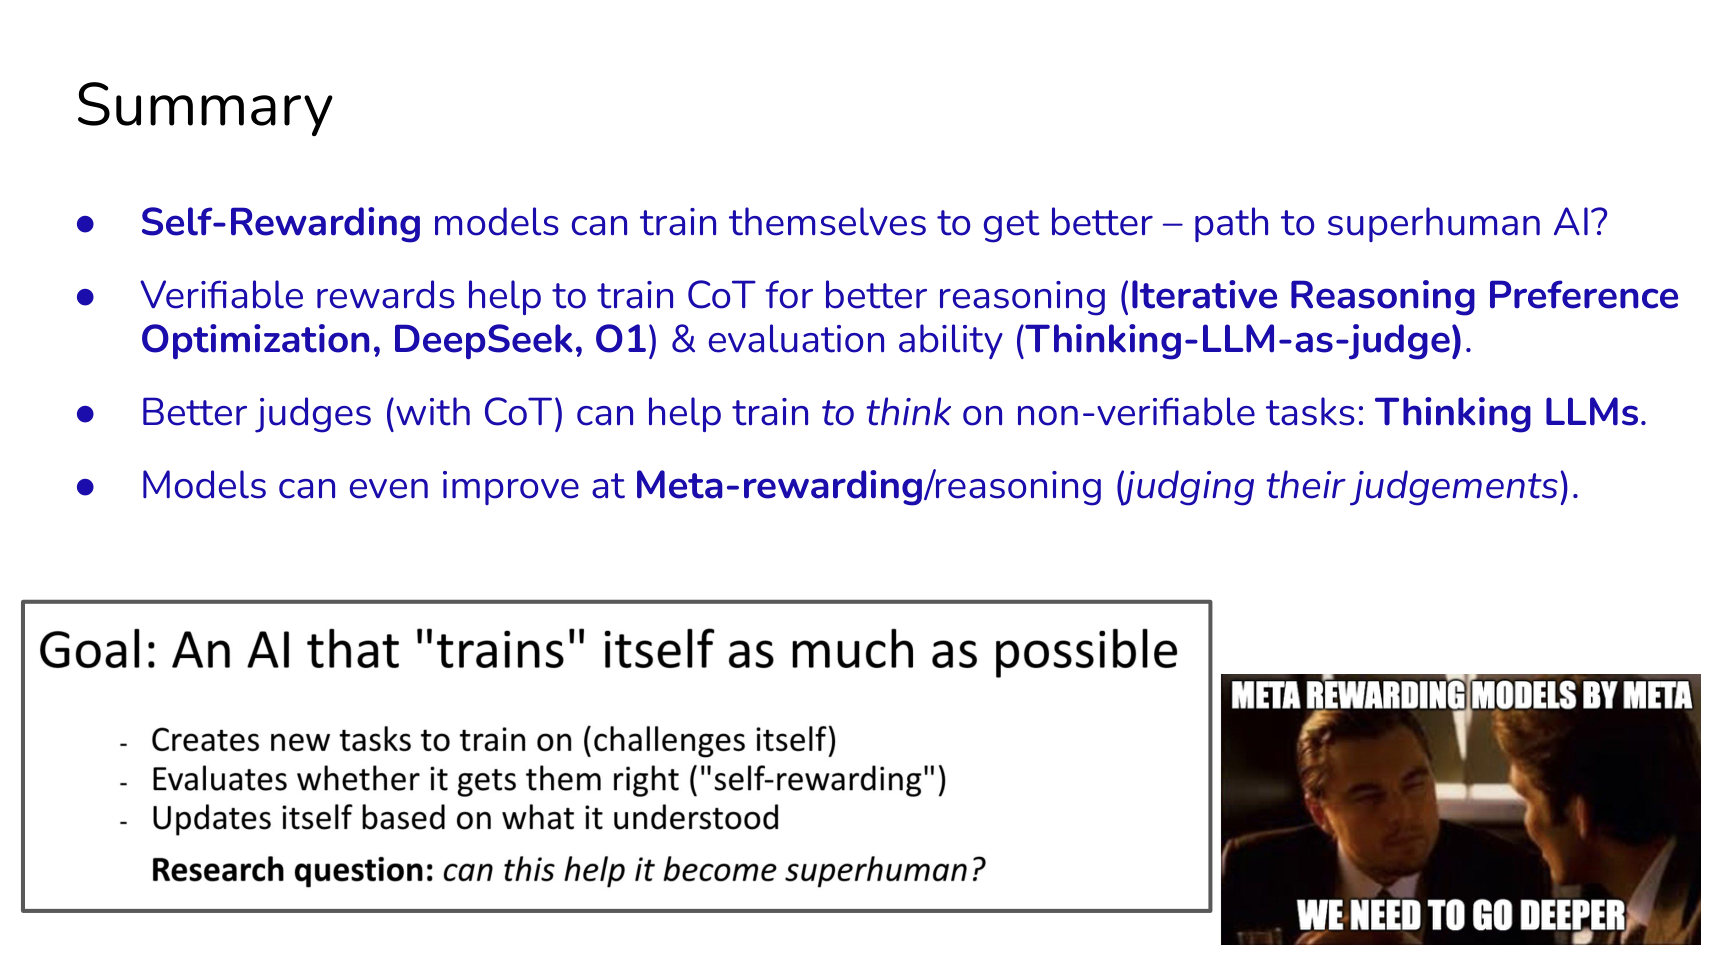
\includegraphics[width=0.76\textwidth]{../lectures/lec02_learning_to_reason/figures/lec02_fig_013.png}
\caption{本讲 summary：reasoning learning 的升级路线，最终都回到了 reward / judgment 是否足够可靠。}
\end{figure}

Weston 这讲最大的贡献，是把“learning to reason”重新写成了“learning to generate better judgments”。其逻辑链条非常清楚：
\begin{itemize}
\item LLM 的 System 1 失败暴露了显式验证与去偏的必要性。
\item 标准 RLHF 的 humans-in-the-loop 无法无限扩展。
\item Self-Rewarding 让 actor 和 judge 一起成长。
\item IRPO 说明 reasoning task 需要可验证 final answer 和 reasoning-specific preference pairs。
\item Meta-Rewarding 与 EvalPlanner 进一步指出：judge 本身也是需要 reasoning 和训练的对象。
\end{itemize}

如果把本讲压缩成一句话，那就是：
\begin{center}
\emph{要让模型学会推理，先得让系统学会更可靠地判断什么才算好的推理。}
\end{center}

\section{复习题}

\begin{enumerate}
\item Weston 为什么把 hallucination、sycophancy、jailbreaking 都归为 System 1 failure？
\item CoVe 与单纯多采样 CoT 的核心差别是什么？
\item DPO 为什么只是 reasoning learning 的“执行器”，而不是完整答案？
\item Self-Rewarding 模型为什么必须同时提升 acting 和 judging 两种能力？
\item IRPO 为什么需要 verifiable final answer 与 negative examples？
\end{enumerate}

\section{深入思考题}

\begin{enumerate}
\item 如果一个任务没有明确 final answer，只能得到模糊的人类评分，你会怎样改写 IRPO 的 reward grounding？
\item Meta-Rewarding 是否会陷入“judge judge judge”的无限回归？系统需要在哪一层停下来并重新接入外部 ground truth？
\item 对真实 agent 环境而言，judge 最终应该主要依赖静态 benchmark、环境反馈，还是人类交互？为什么？
\end{enumerate}

\section{延伸阅读}

\begin{itemize}
\item \textbf{DPO}：理解为什么 KL-constrained RLHF 可以直接化为 preference optimization。
\item \textbf{IRPO}：理解 reasoning preference pair 的构造方式，以及为什么 NLL 项不能轻易拿掉。
\item \textbf{CoVe}：理解 verification planning 在 factuality 问题中的作用。
\item 如继续深入本门课，可将本讲与第一讲的 verifier、Self-Debugging，以及后续 memory / planning 章节一起阅读，形成“生成-评价-修正”的统一视角。
\end{itemize}

\chapter{On Reasoning, Memory, and Planning of Language Agents}
\label{chap:lec03_reasoning_memory_planning}
\section{本讲学习目标}

第三讲的任务不是再介绍一个局部 prompting trick，而是为整门课提出一个更宽的对象：\textbf{language agents}。Yu Su 的观点是，当前这波 agent 之所以值得重新讨论，不是因为它们能说更多话，而是因为语言本身正在变成一种用于\textbf{推理（reasoning）、记忆组织（memory organization）、规划（planning）和多模块协调}的通用表示层。

读完本讲后，读者应能回答：
\begin{itemize}
\item 为什么 Yu Su 主张使用 “language agent” 这个术语，而不是把一切都塞进笼统的 AI agent 桶里。
\item 为什么当前 RAG 还不足以支撑长期记忆，HippoRAG 试图补什么。
\item 什么叫 implicit reasoning，为什么 Grokked Transformers 说明“没有显式 CoT 不等于没有推理”。
\item WebDreamer 为什么代表了 language-agent planning 从 reactive execution 走向 model-based planning 的关键转折。
\item memory、reasoning 和 planning 为什么必须一起设计，而不能孤立优化。
\end{itemize}

\section{背景与统一框架}

\subsection{为什么又是 agents}

Yu Su 用经典定义重新开场：agent 是能够通过传感器感知环境、并通过执行器对环境施加动作的系统。把这一定义代入当代 LLM，就会立刻发现一个变化：模型不再只处理纯文本输入输出，而是位于感知、动作、反思与环境反馈之间的闭环中。

\begin{figure}[H]
\centering
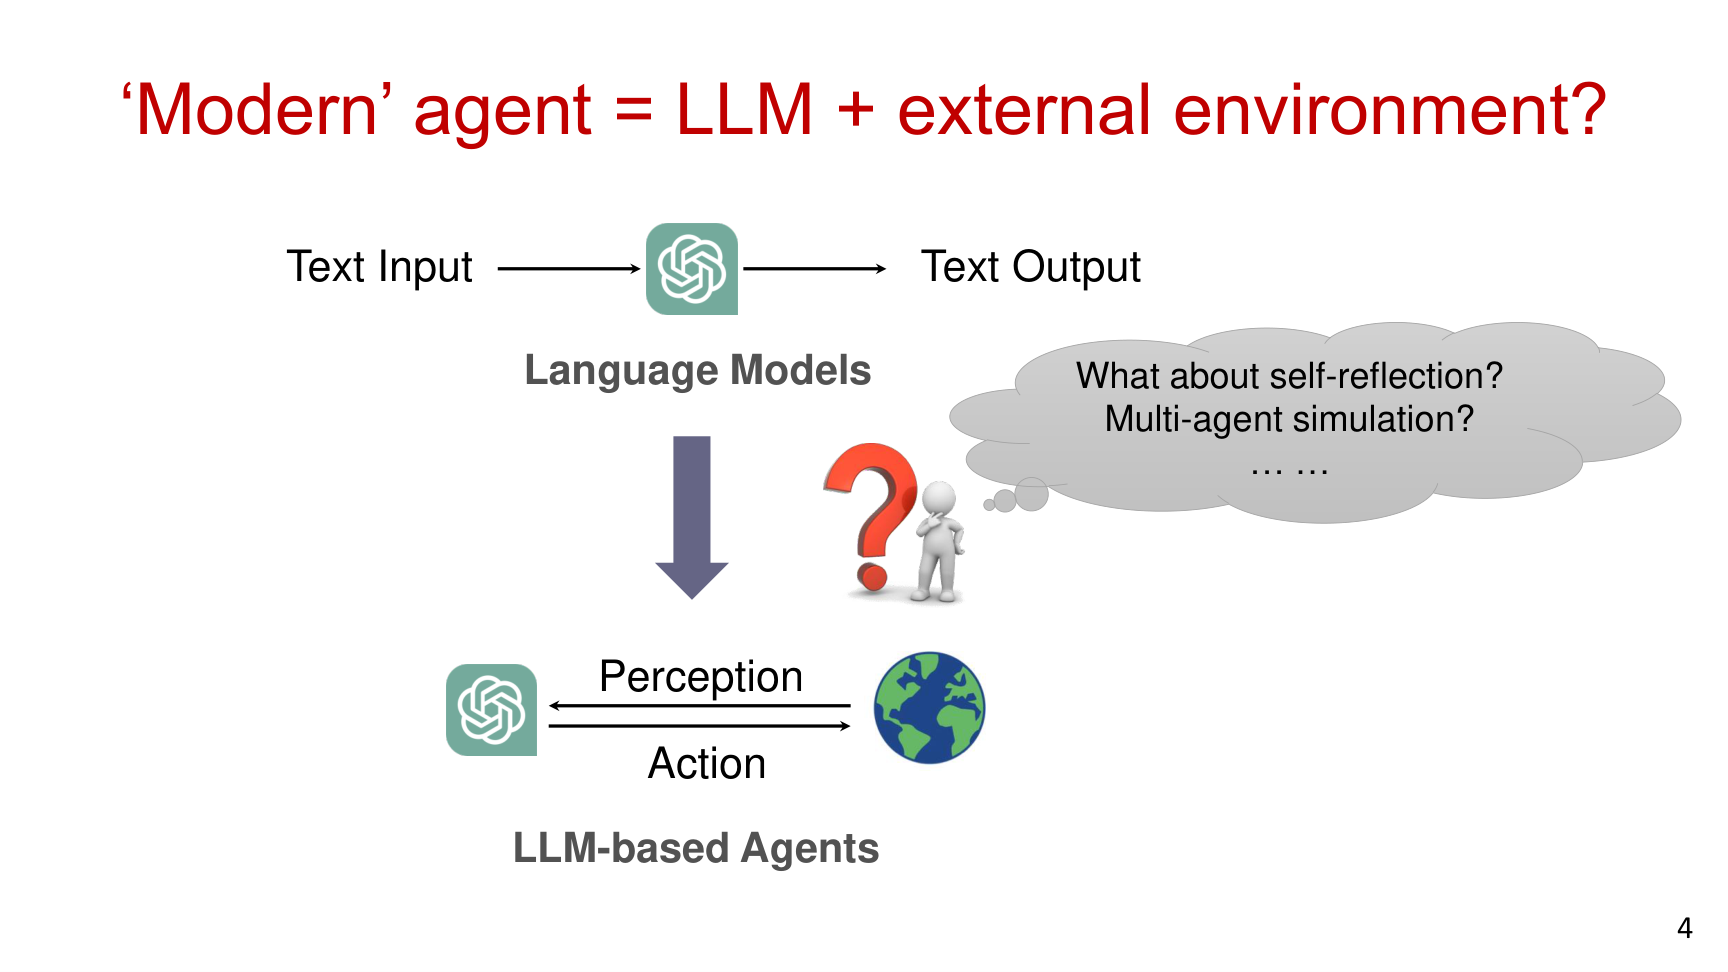
\includegraphics[width=0.82\textwidth]{../lectures/lec03_reasoning_memory_planning/figures/lec03_fig_001.png}
\caption{语言 agent 的最小闭环：perception、reasoning、action、self-reflection 和 environment feedback 共同构成 agent workflow。}
\end{figure}

这意味着“reasoning”本身也要重新定义。对语言 agent 来说，生成 token 不只是在输出答案，也可以是\textbf{内部动作（internal action）}：写计划、写状态假设、做自我反思、生成候选未来状态。这就是 Yu Su 强调 inner monologue 的原因。

\subsection{LLM-first 与 agent-first}

Lecture 中一个非常有用的区分是：
\begin{itemize}
\item \textbf{LLM-first view}：先有 LLM，再往上堆记忆、工具和 prompt scaffold，让它看起来像 agent。
\item \textbf{Agent-first view}：先从 agent 所需能力出发，再把 LLM 作为 reasoning / communication module 整合进去。
\end{itemize}

前者更贴近当下工程实践，后者更接近长期研究路线。Yu Su 没有简单否定任何一方，而是指出两者在系统设计中同时存在：今天的 agent 既是 prompt-heavy engineering artifact，也是朝着更完整智能体过渡的原型。

\subsection{为什么叫 language agent}

讲者用 logical agent、neural agent 和 language agent 的对比图强调：language agent 的突出特征不是它“更智能”，而是它拥有更高的\textbf{表达能力（expressiveness）}。逻辑 agent 很严谨但语言受限，纯神经 agent 可以编码很多模式但难以显式沟通，而 language agent 能用自然语言组织状态、理由、计划和工具调用。

\begin{figure}[H]
\centering
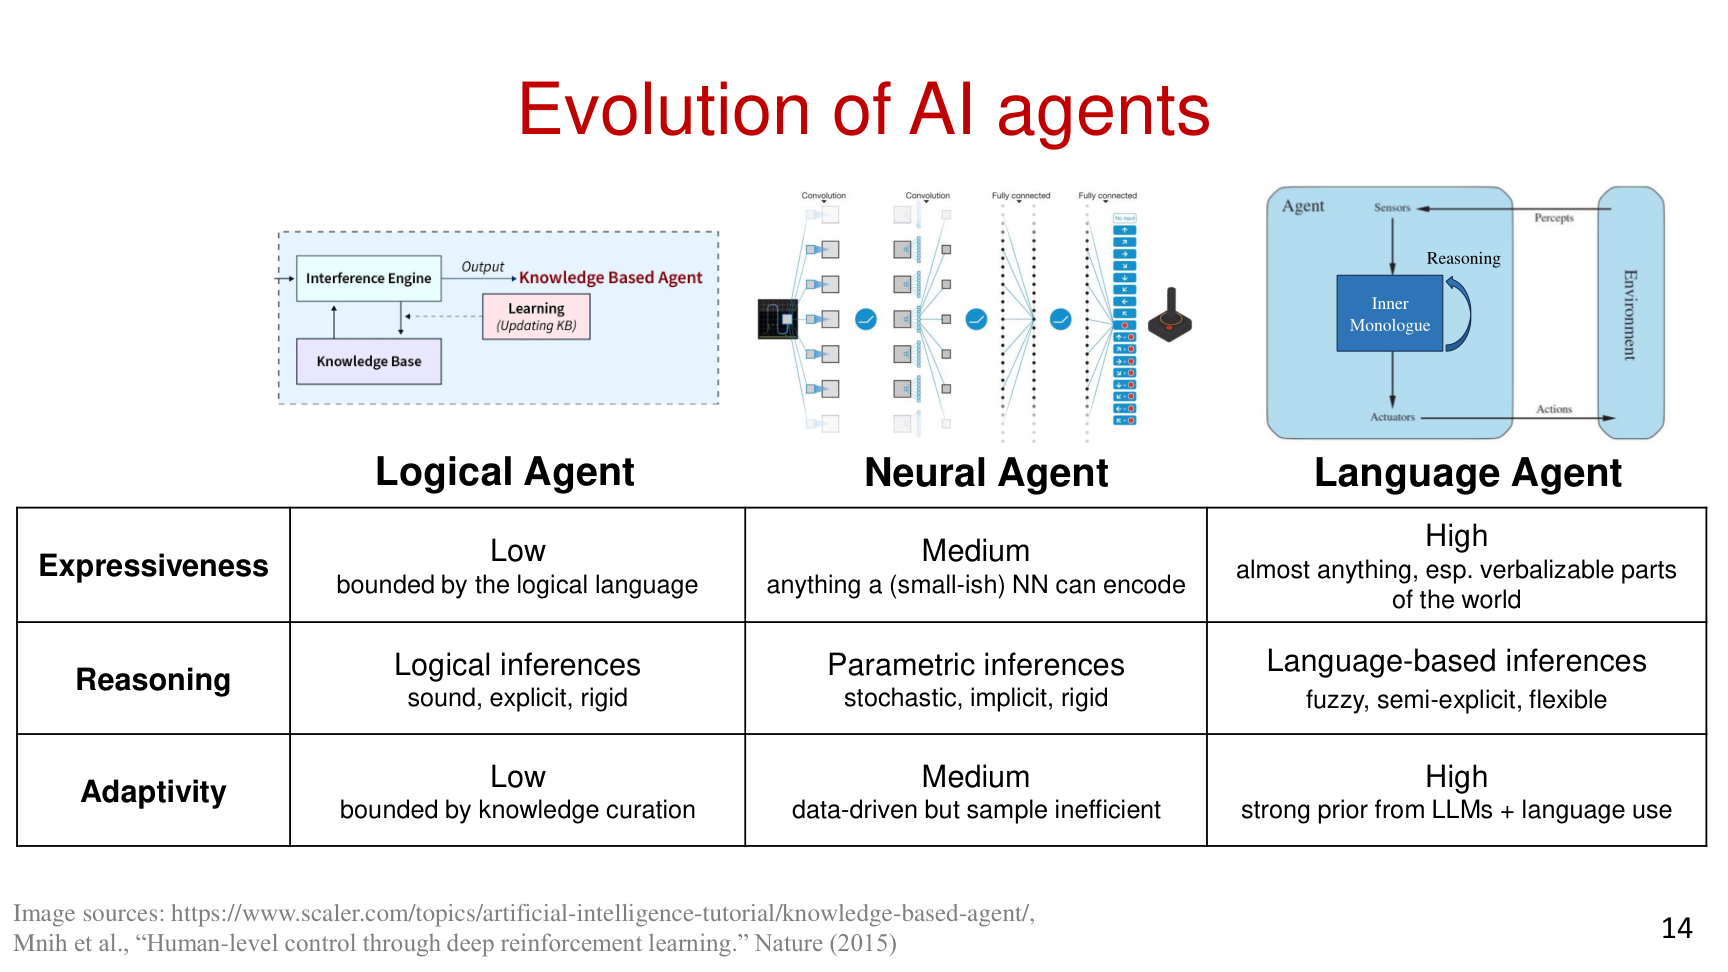
\includegraphics[width=0.78\textwidth]{../lectures/lec03_reasoning_memory_planning/figures/lec03_fig_002.png}
\caption{Logical / Neural / Language Agent 的对比：language agent 的核心优势是高表达性，这也解释了它为什么适合 reasoning、memory 和 planning 的协调。}
\end{figure}

\begin{knowledgebox}{本讲的统一视角}
语言不是附属接口，而是 language agent 的核心组织媒介。它既承载内隐或显式推理，也承载记忆索引、规划、协调、工具调用和人机沟通。
\end{knowledgebox}

\section{长期记忆：为什么当前 RAG 还不够}

\subsection{RAG 的问题不是“检索不够快”，而是“记忆结构太浅”}

Yu Su 用一个多跳问答案例说明当前 RAG 的典型失败：问题需要在多条知识之间做联想和桥接，但普通 dense retrieval 只会优先找到表面相似的片段，而不擅长 reconstruct deeper associations。

\begin{figure}[H]
\centering
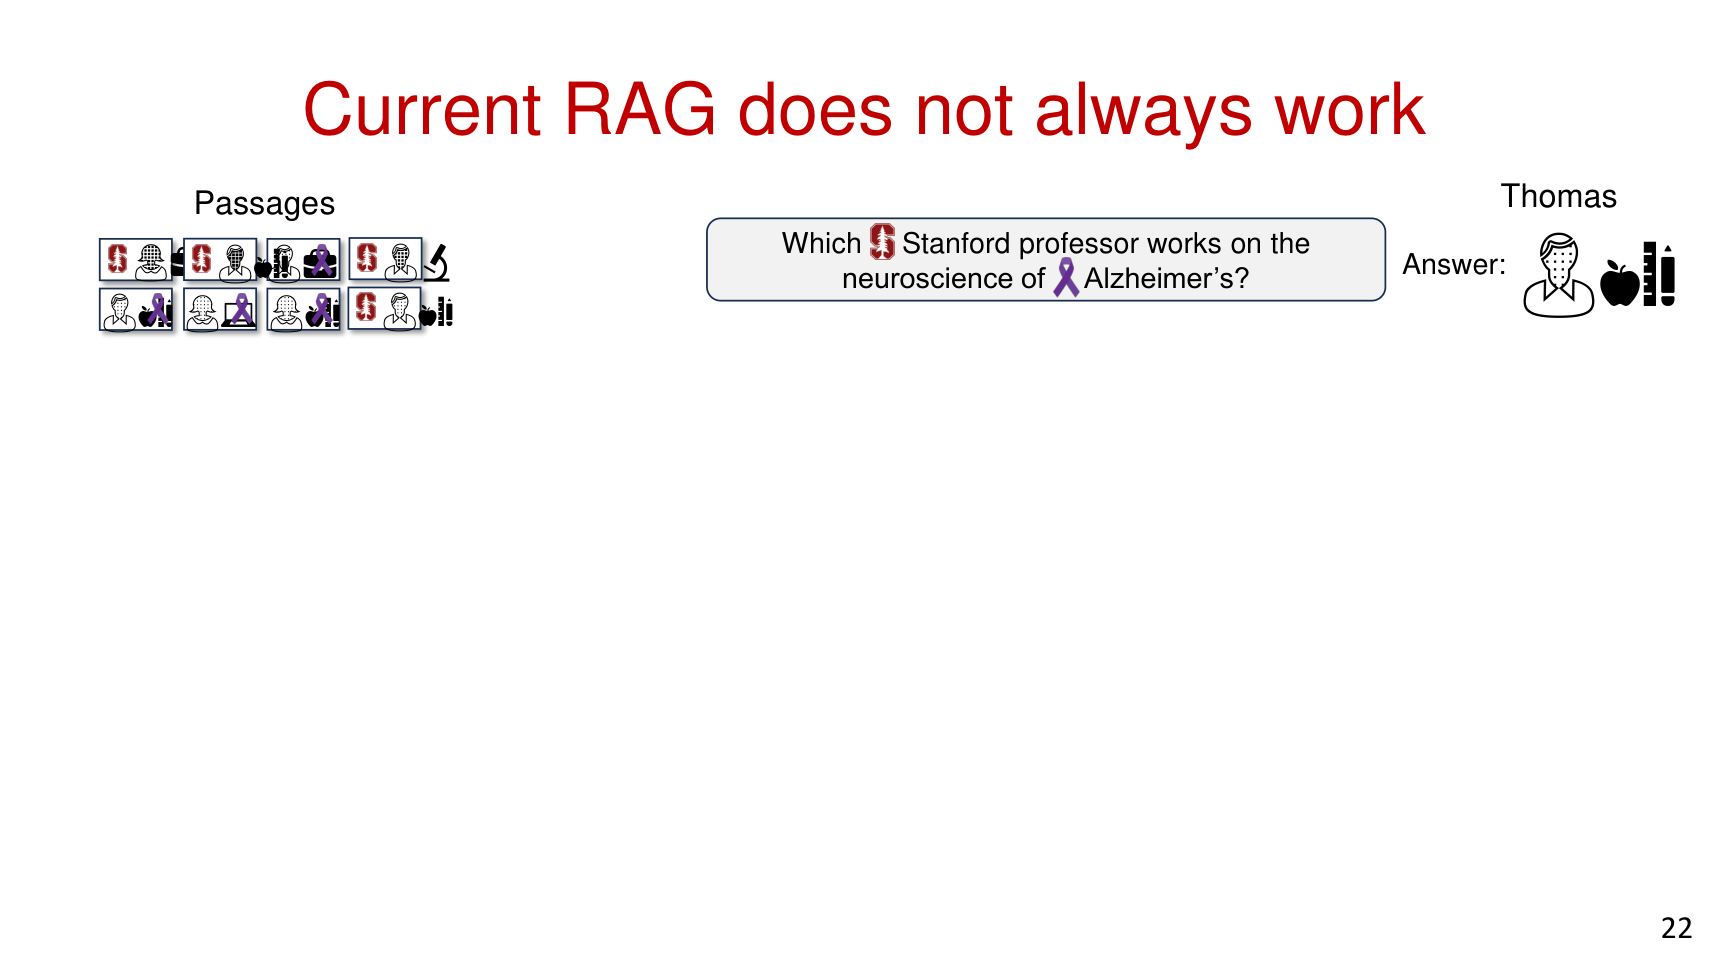
\includegraphics[width=0.78\textwidth]{../lectures/lec03_reasoning_memory_planning/figures/lec03_fig_003.png}
\caption{当前 RAG 的失败案例：多跳记忆问题被错误地退化成浅层相似性检索。}
\end{figure}

这意味着 language agent 的 memory 设计不能只停留在“外挂一些文档块然后 top-k 检索”。真正困难的是：\textbf{如何把新经验组织成可以联想、可恢复、可重组的 memory substrate。}

\subsection{HippoRAG：把长期记忆做成索引与联想系统}

HippoRAG 的核心灵感来自 hippocampal indexing theory。这个理论认为，海马体并不把完整记忆原样储存成单个块，而是维护索引以及记忆之间的联想关系，从而支持 pattern separation 和 pattern completion。

\begin{figure}[H]
\centering
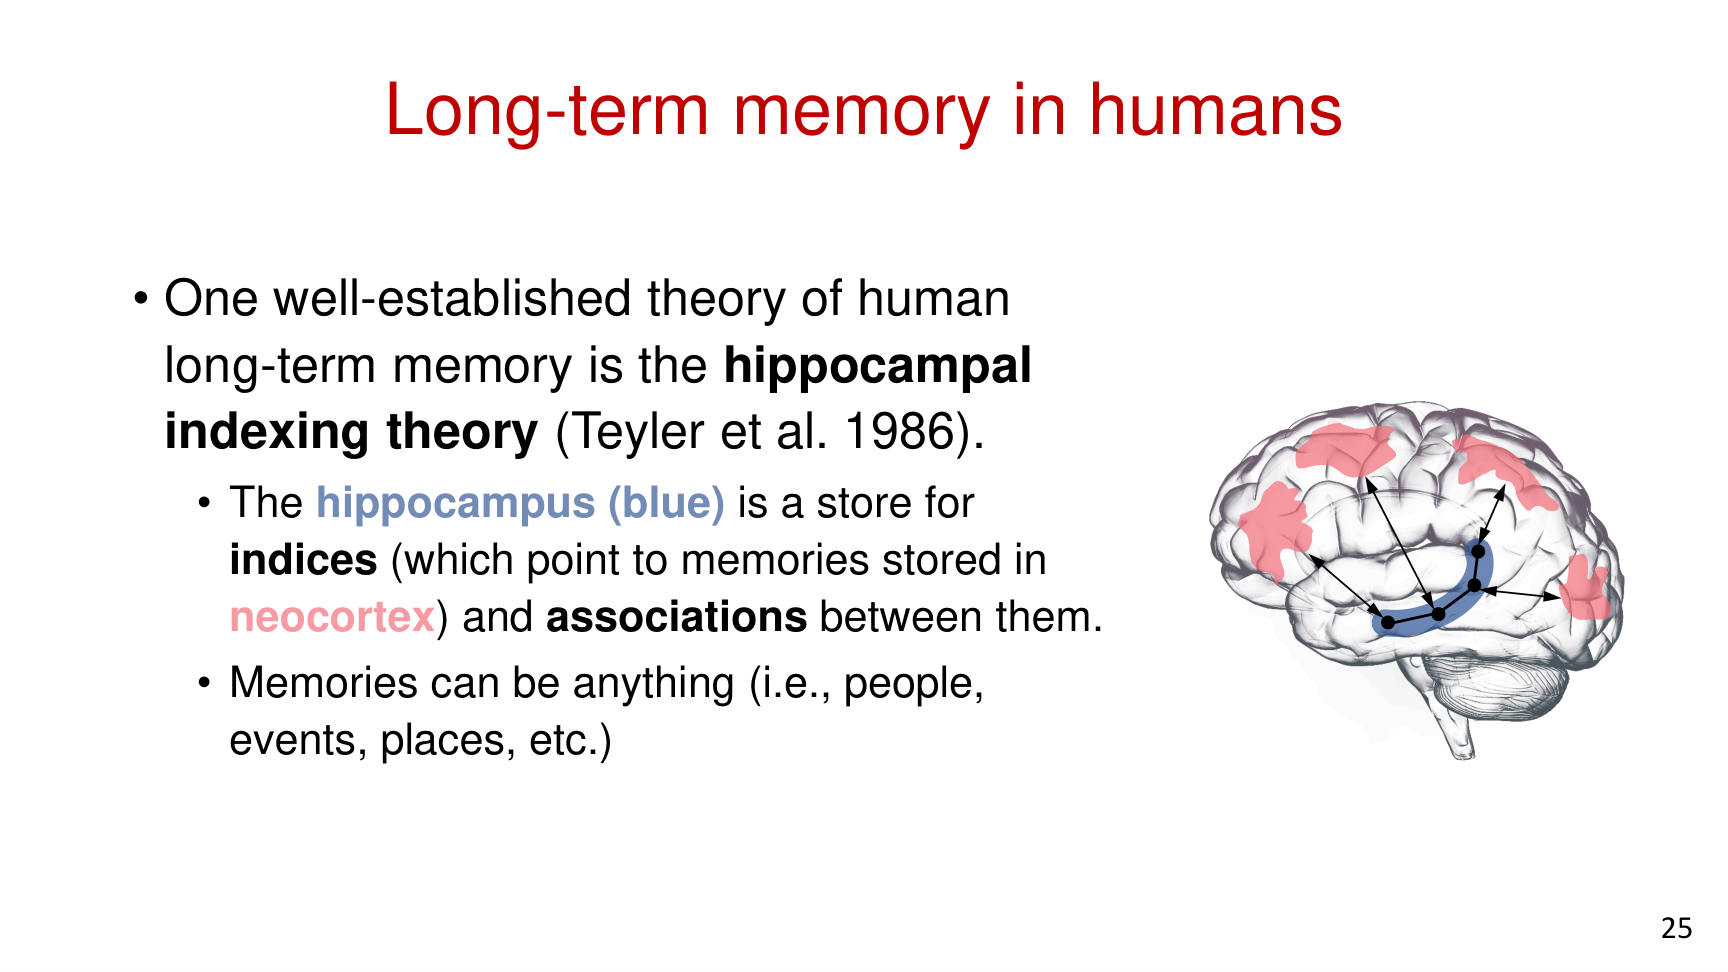
\includegraphics[width=0.74\textwidth]{../lectures/lec03_reasoning_memory_planning/figures/lec03_fig_004.png}
\caption{HippoRAG 的认知灵感：长期记忆不是只靠相似度召回，而是靠索引和联想结构恢复。}
\end{figure}

这给语言 agent 一个关键启示：如果记忆是图结构而不是平铺 chunk 列表，那么 retrieval 就不仅是“哪个段落最像 query”，而是“从哪些锚点出发，沿哪些关系扩散，才能恢复与当前任务相关的完整记忆”。

HippoRAG 用知识图、LLM 和 Personalized PageRank 来实现这一点。一个简化写法是：
\[
\mathbf{r}=\alpha \mathbf{e}_q + (1-\alpha)\mathbf{P}^{\top}\mathbf{r}
\]
这里 $\mathbf{e}_q$ 是由查询初始化的 personalization 向量，$\mathbf{P}$ 是知识图转移矩阵，$\mathbf{r}$ 是最终 memory relevance 分布，$\alpha$ 控制查询锚点与图扩散之间的权衡。

\paragraph{直觉解释}
普通 RAG 更像“把问题拿去最近邻检索”；HippoRAG 更像“先找到与问题相关的记忆入口，再沿着联想路径逐渐恢复整片相关记忆结构”。

\begin{figure}[H]
\centering
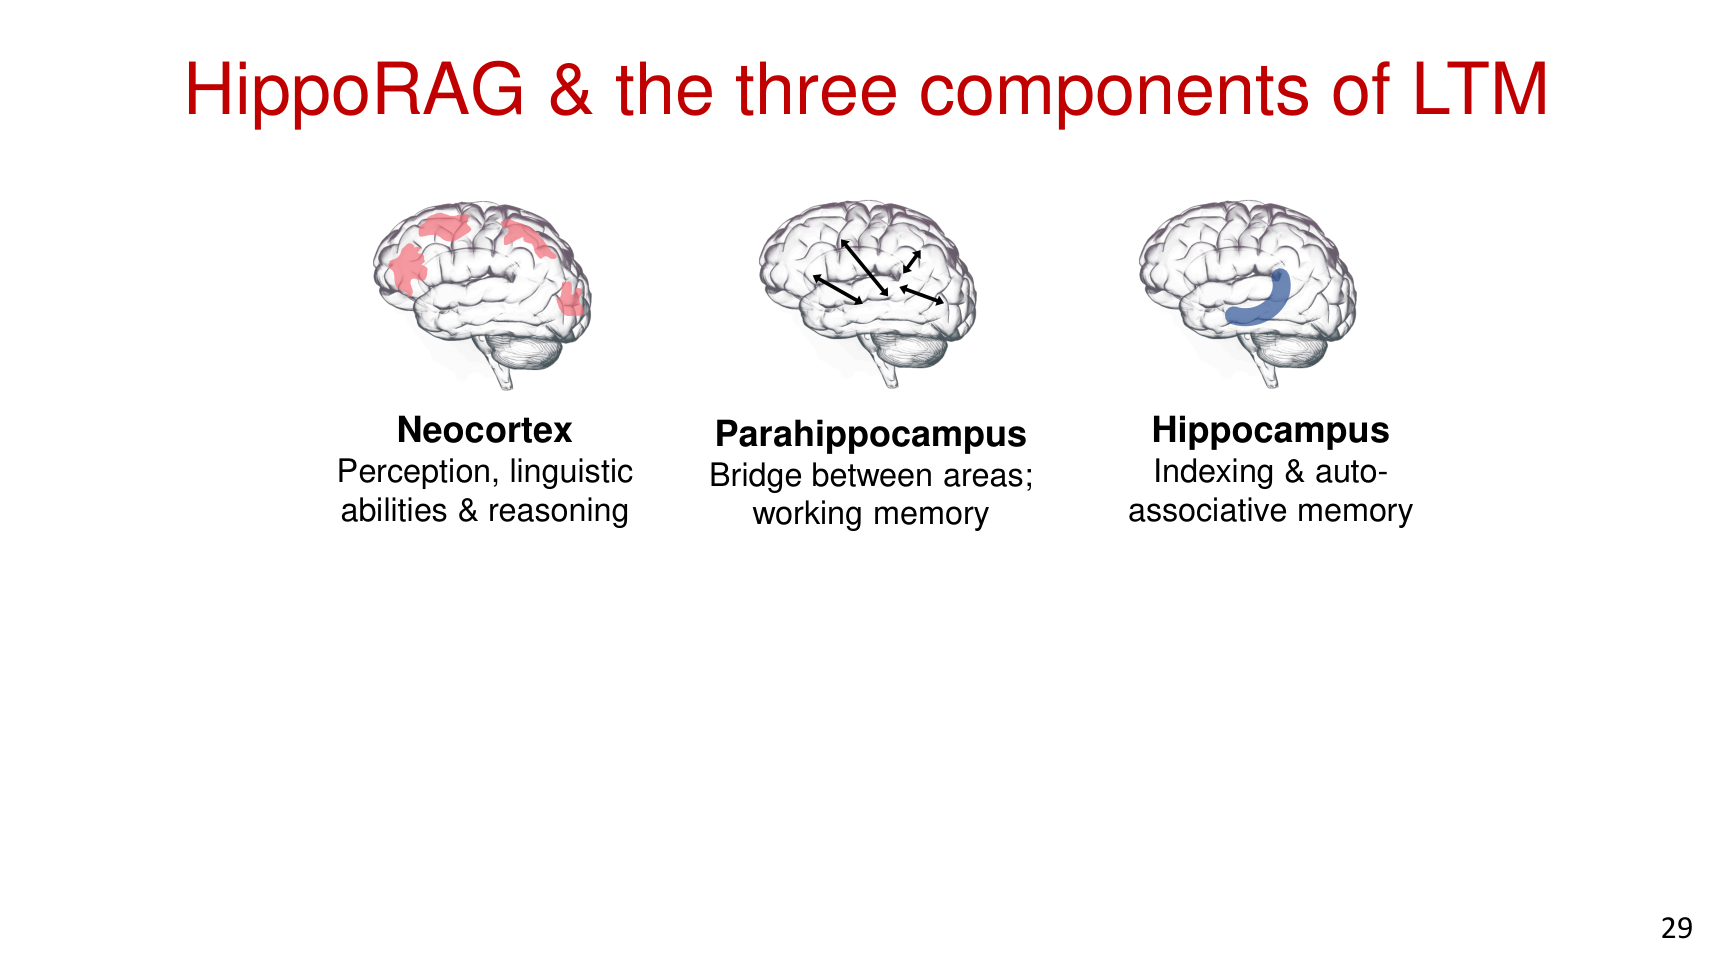
\includegraphics[width=0.80\textwidth]{../lectures/lec03_reasoning_memory_planning/figures/lec03_fig_005.png}
\caption{HippoRAG 的三个部件：知识存储、桥接与索引-联想机制共同组成长期记忆检索系统。}
\end{figure}

\begin{lstlisting}
Build a graph over entities, passages, and relations
Seed query-relevant nodes from the current question
Run Personalized PageRank over the graph
Retrieve passages associated with the highest-scoring memory nodes
\end{lstlisting}

\paragraph{为什么这对 agent 很关键}
对 language agent 来说，记忆不是只服务单轮问答。它还要支撑个性化、持续学习、多步任务和跨时空的关联恢复。没有更好的记忆结构，agent 很容易每轮都像第一次见到世界。

\subsection{HippoRAG 的实验结果与边界}

HippoRAG 在多跳问答上明显优于常见 RAG baselines，也往往比迭代检索更便宜。这说明非参数记忆并不是无用，而是要设计得像\textbf{联想记忆系统}，而非简单文本外挂。

\begin{figure}[H]
\centering
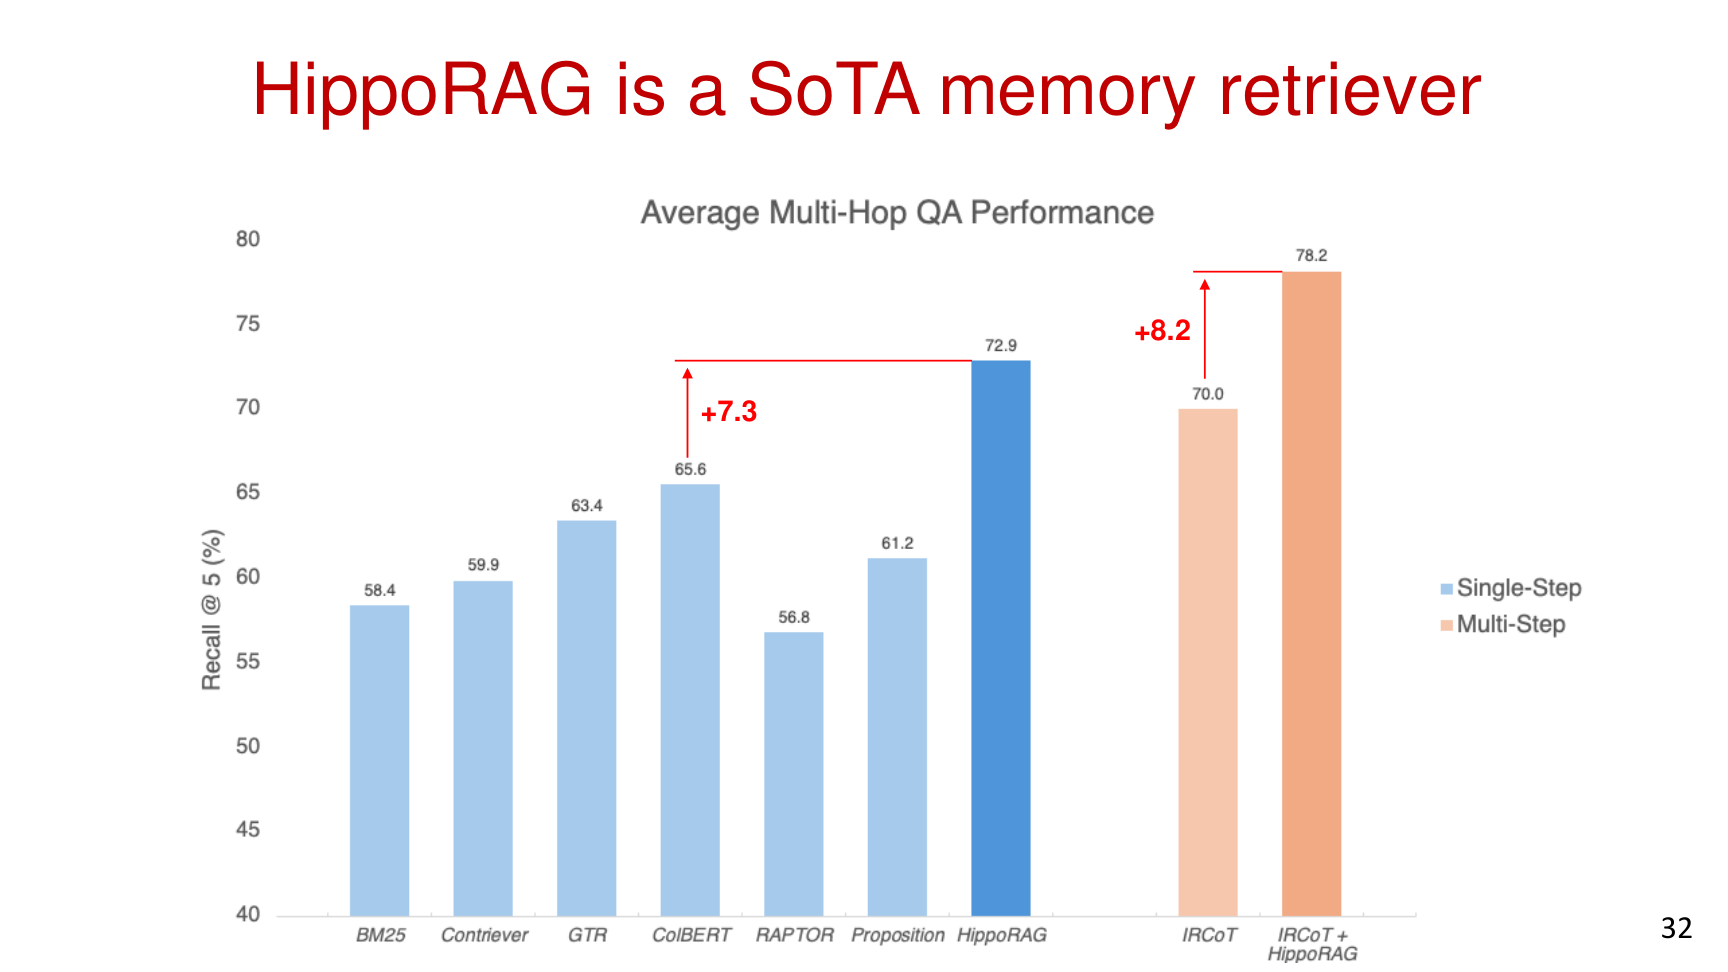
\includegraphics[width=0.72\textwidth]{../lectures/lec03_reasoning_memory_planning/figures/lec03_fig_006.png}
\caption{HippoRAG 的结果页：记忆检索结构本身就会显著影响 reasoning quality。}
\end{figure}

但讲者也没有把它说成完整答案。HippoRAG 仍然主要解决“如何更好地取回长期记忆”，并不自动解决 continual learning、memory editing、personalization safety 等更广问题。它是 memory module 的强基线，而不是终局。

\section{推理：显式 CoT 之外，implicit reasoning 依然重要}

\subsection{为什么要讨论 implicit reasoning}

当整个社区都在关注 CoT 时，Yu Su 反过来问：没有 verbalized thoughts 的 transformer，是否也能通过参数内部结构学会推理？这就是 Grokked Transformers 的研究对象。

\begin{figure}[H]
\centering
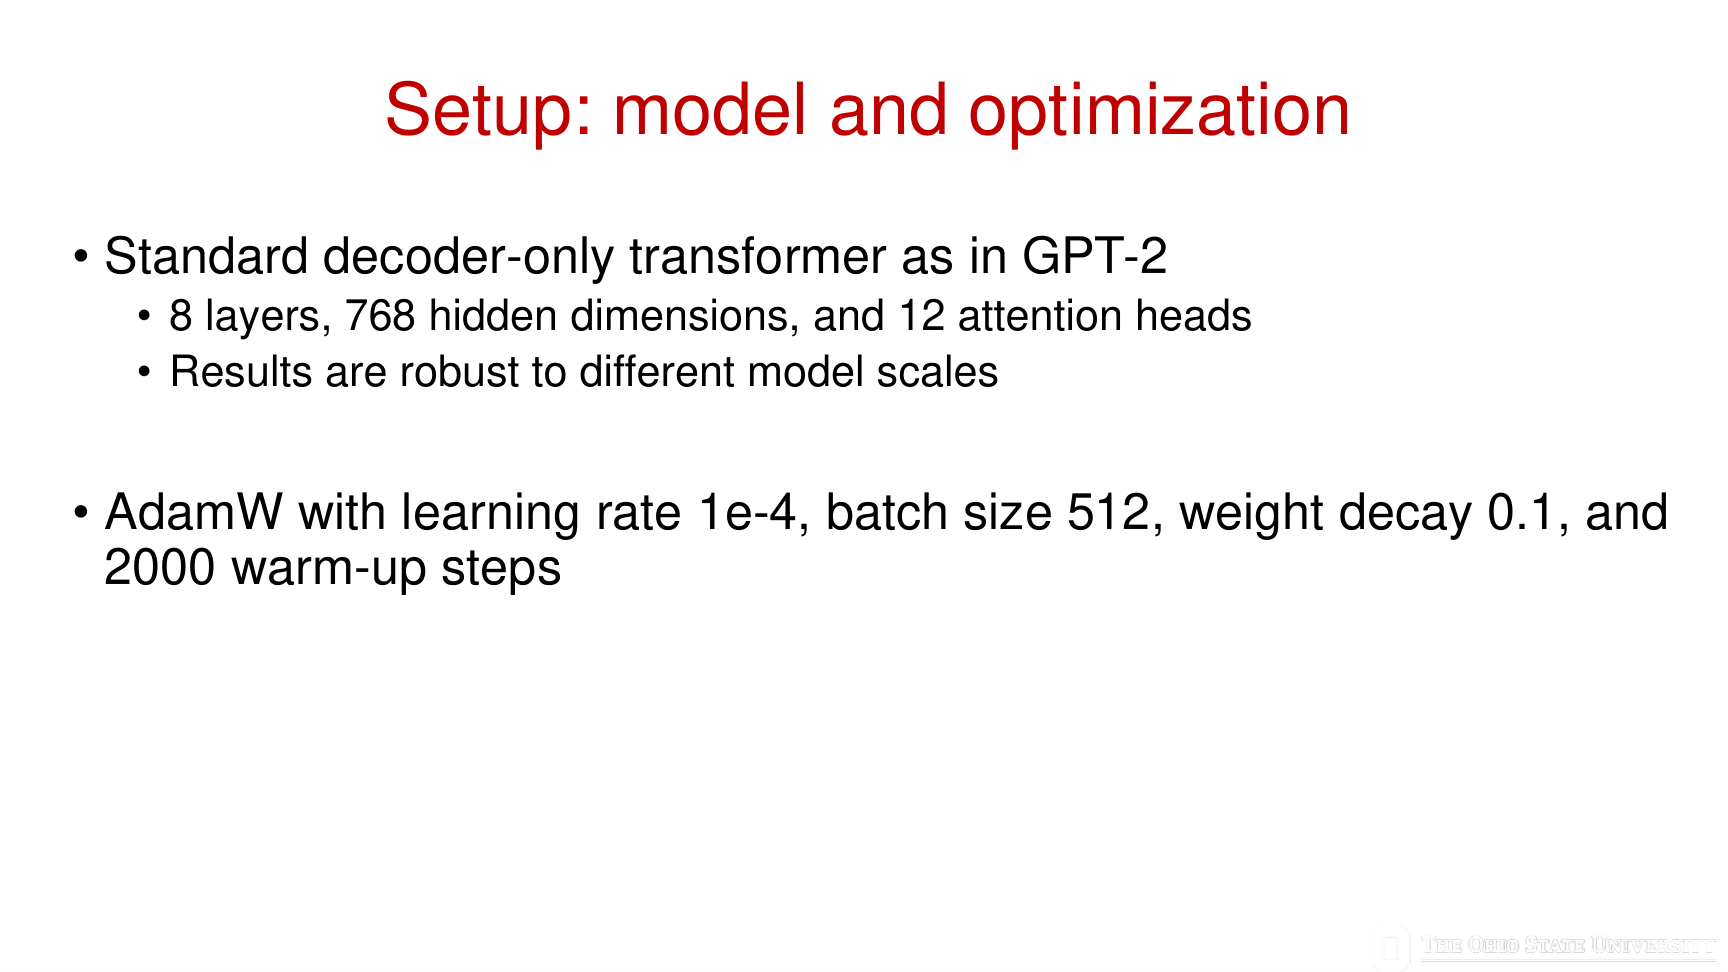
\includegraphics[width=0.80\textwidth]{../lectures/lec03_reasoning_memory_planning/figures/lec03_fig_007.png}
\caption{Grokked Transformers 的实验设置：通过可控合成任务，单独研究 implicit reasoning 的学习与泛化。}
\end{figure}

这里的重点是，language agents 的 reasoning 不应该被误解为“只要会写 CoT”。在很多时候，显式 CoT 是\textbf{外显接口}，而真正的结构化表征学习仍然发生在模型参数与电路层面。若忽略这一点，就会把推理能力过度等同于解释能力。

\subsection{Grokking：从记忆回放到泛化相变}

Grokked Transformers 研究显示，transformer 可以学会 implicit reasoning，但往往要经历 grokking：也就是在训练误差早已很低之后，继续训练很久，模型才从 memorization 过渡到真正 generalization。

\begin{figure}[H]
\centering
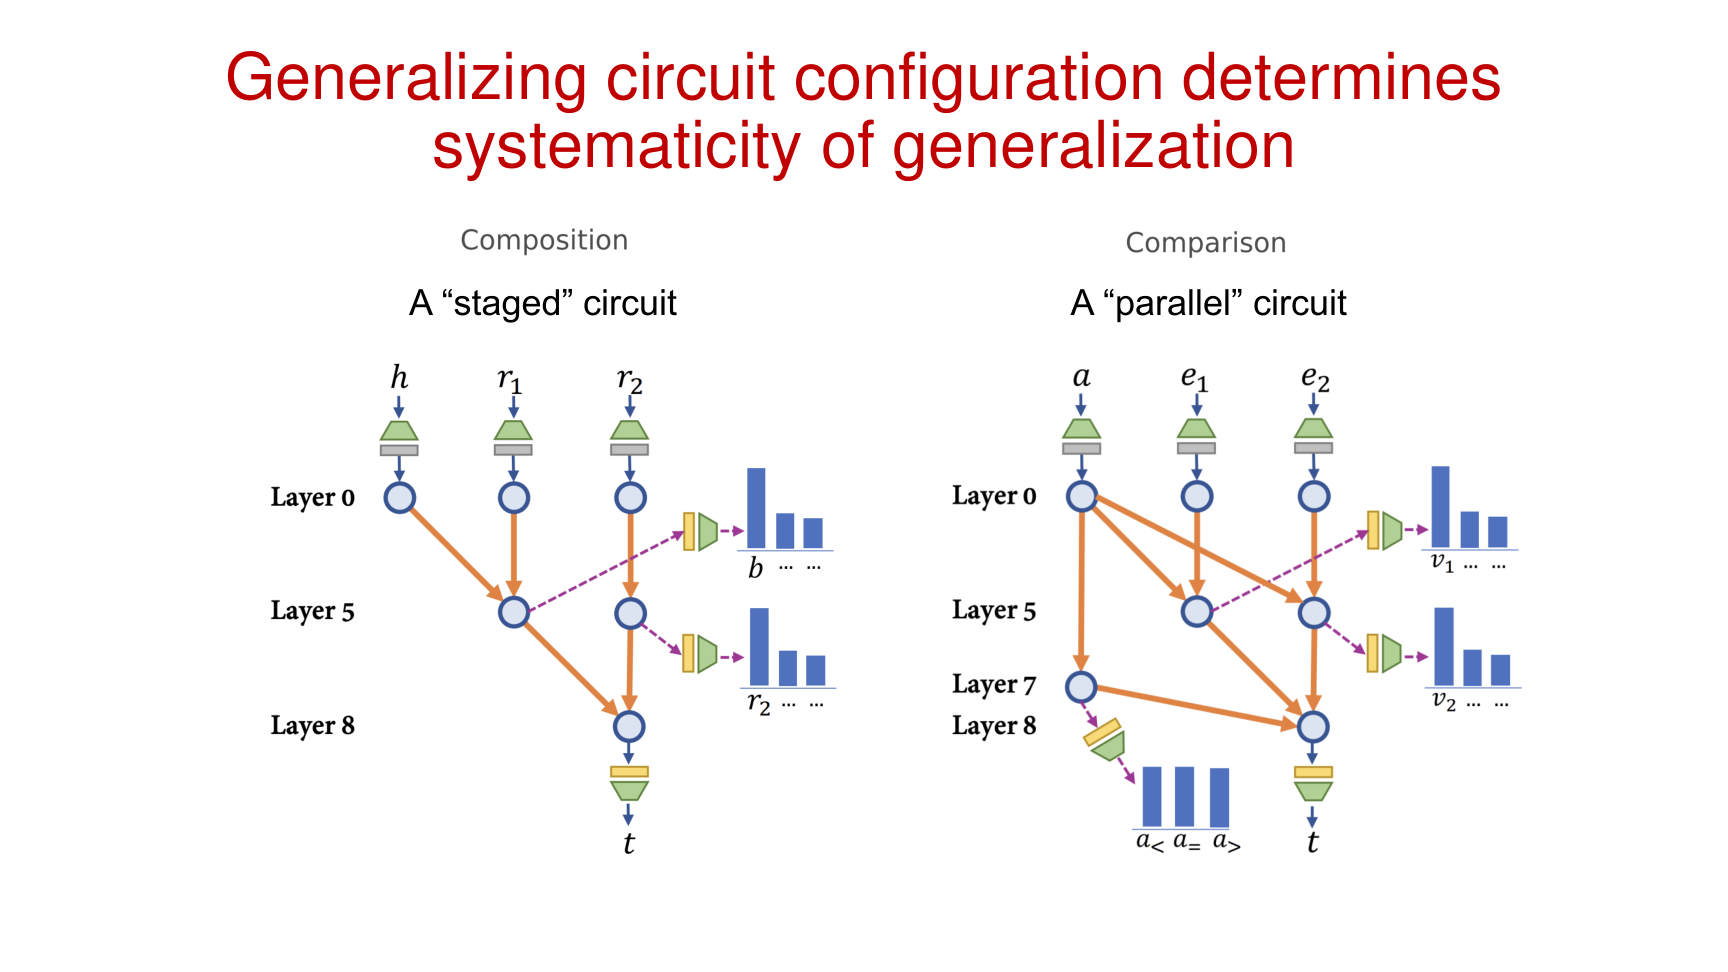
\includegraphics[width=0.78\textwidth]{../lectures/lec03_reasoning_memory_planning/figures/lec03_fig_008.png}
\caption{generalizing circuit 的配置决定 systematicity：不同 reasoning type 会形成不同的内部电路结构。}
\end{figure}

\begin{figure}[H]
\centering
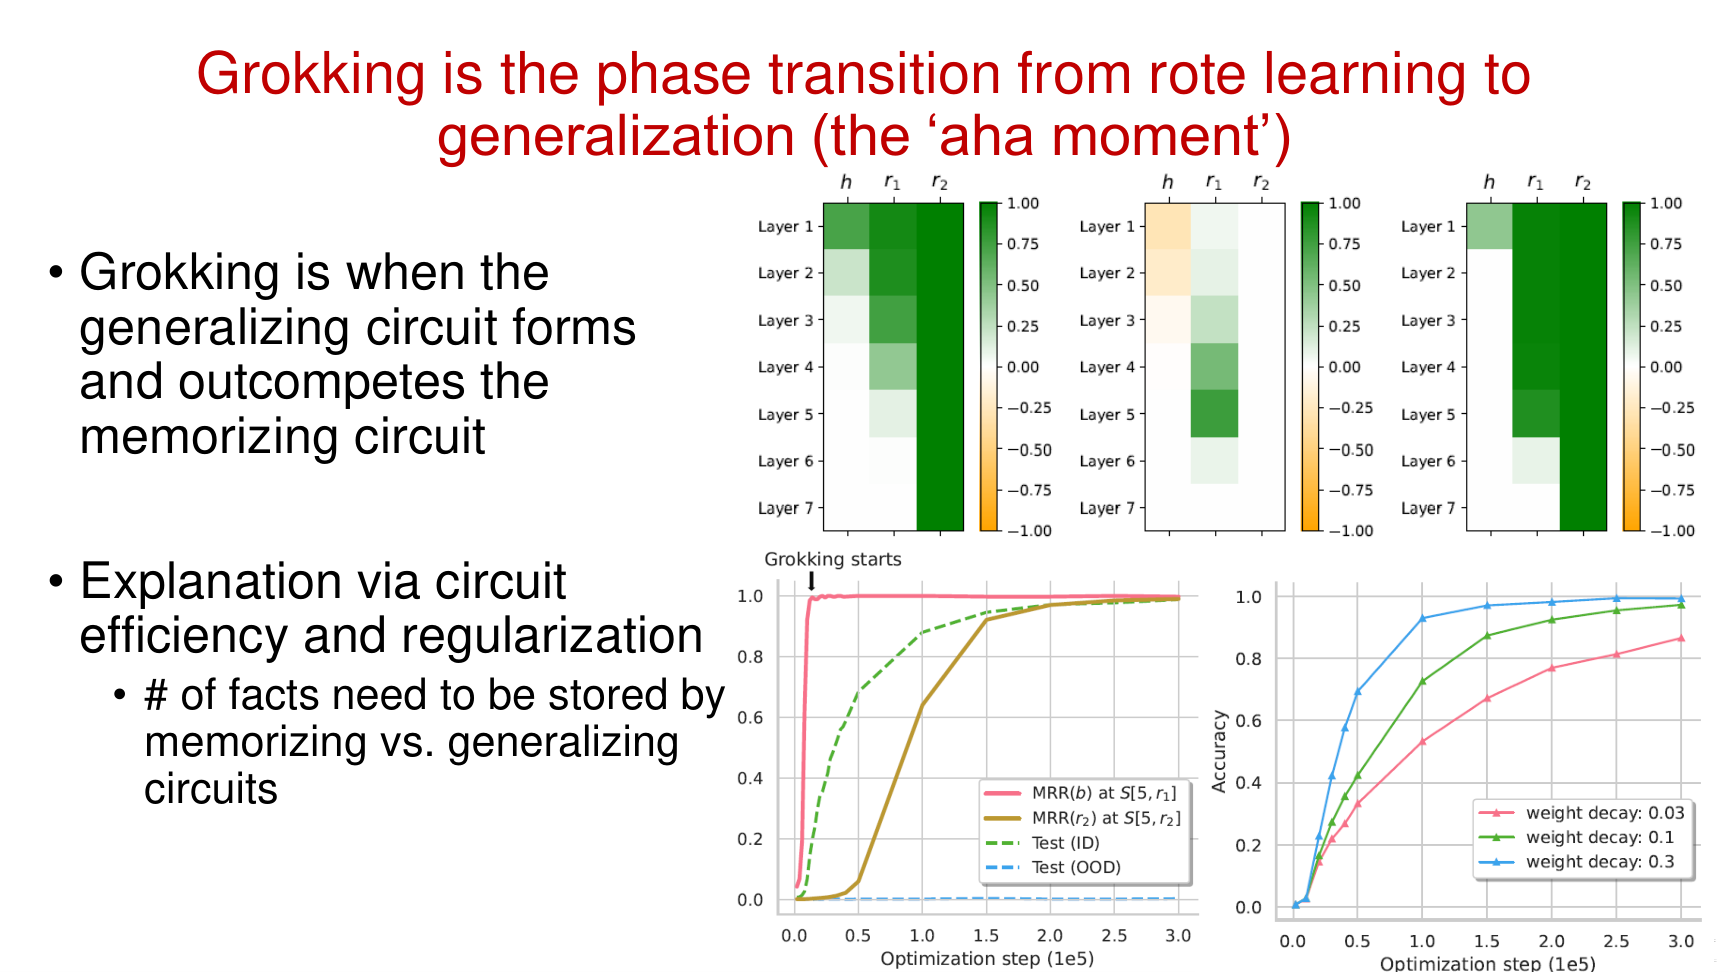
\includegraphics[width=0.78\textwidth]{../lectures/lec03_reasoning_memory_planning/figures/lec03_fig_009.png}
\caption{Grokking 被讲成从 rote memorization 向 systematic generalization 的相变。}
\end{figure}

\begin{lstlisting}
Train the transformer far beyond interpolation
Probe intermediate representations with a logit lens
Run causal tracing to identify memorizing and generalizing circuits
Compare circuit configurations across reasoning types
\end{lstlisting}

\paragraph{为什么这件事与 language agents 有关}
因为很多 agent 成功与否，取决于模型是否已经学会某种\textbf{隐式结构能力}。如果底层模型连 relations、rules、state abstractions 都没学稳，那么上层再复杂的 planning scaffold 也只是补丁。

\paragraph{一个重要 caveat}
Yu Su 也强调，Grokked Transformers 的证据来自可控 synthetic settings。它告诉我们“这种能力机制存在”，但不意味着大模型在开放世界里已经自动拥有同等稳健的 implicit reasoning。

\section{规划：从 reactive execution 到 model-based planning}

\subsection{Planning setting 已经变了}

传统规划常假定 formal domain、有限动作空间和清晰 goal test。但 language agents 进入 web、travel、GUI 等环境后，goal 用自然语言表达，动作空间开放且状态常带噪声。于是 planning 不再是单纯求解 PDDL，而是要处理含糊目标、开放动作、多模态反馈和昂贵环境交互。

\begin{figure}[H]
\centering
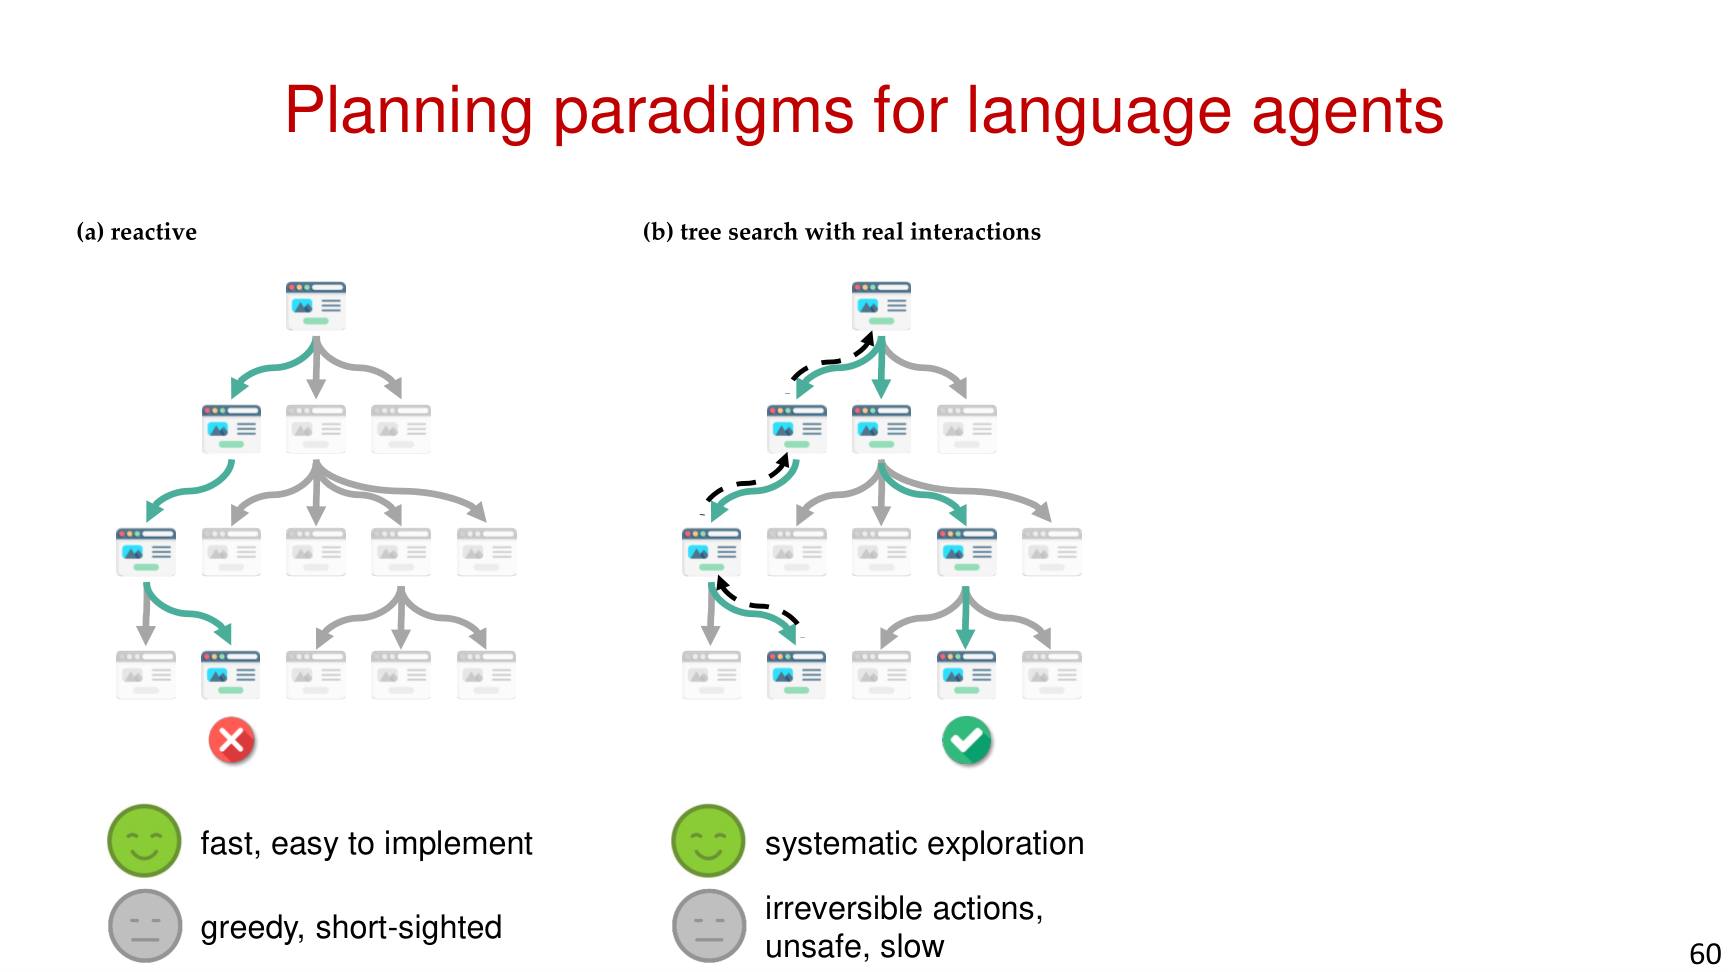
\includegraphics[width=0.78\textwidth]{../lectures/lec03_reasoning_memory_planning/figures/lec03_fig_010.png}
\caption{Planning paradigms 对比：reactive planning 快但短视，tree search 更系统但在真实环境中常太慢、太危险。}
\end{figure}

Yu Su 用 reactive、tree search 与 model-based planning 的比较说明：在真实网页环境里，单纯 tree search 面临三重问题：
\begin{itemize}
\item 很多动作是\textbf{不可逆}的，无法随意 backtrack。
\item 真环境交互带来\textbf{安全和隐私风险}。
\item 在线探索会显著增加 latency 与 cost。
\end{itemize}

\begin{figure}[H]
\centering
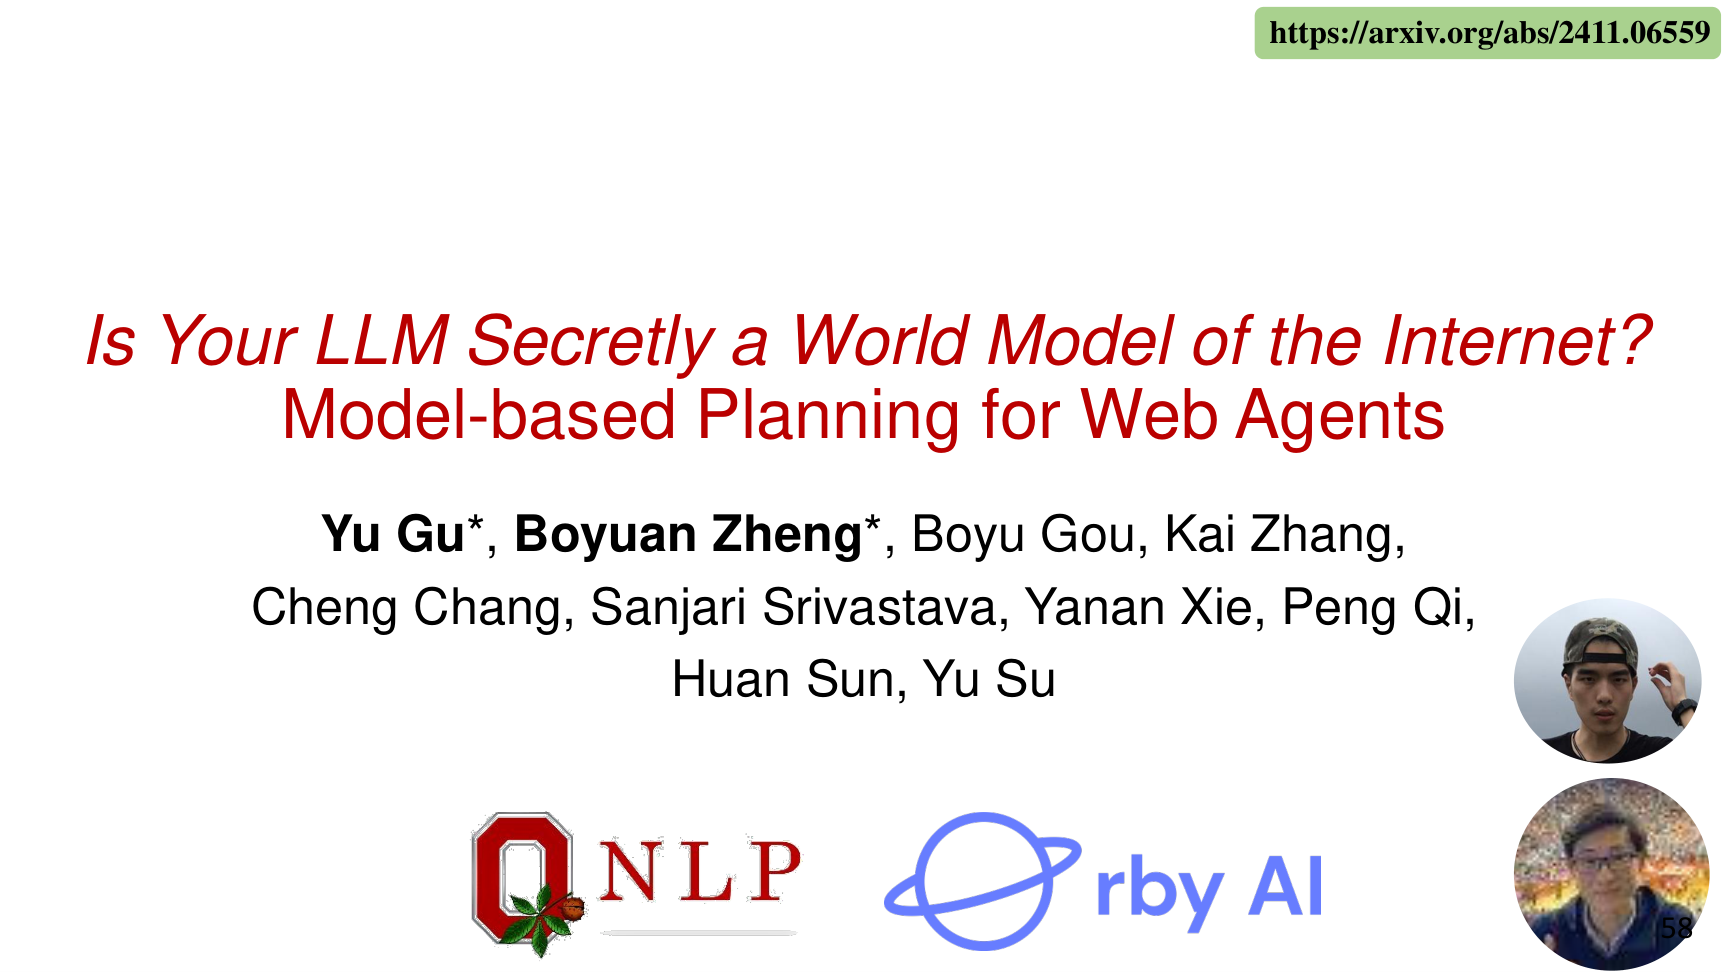
\includegraphics[width=0.76\textwidth]{../lectures/lec03_reasoning_memory_planning/figures/lec03_fig_011.png}
\caption{WebDreamer 连接 benchmark 视角与 planning 视角：web agent 不只是能点网页，而是要在现实约束下做安全高效规划。}
\end{figure}

\subsection{WebDreamer：先在脑内做 imagination，再去网页上行动}

WebDreamer 的关键思想是：既然真实环境探索昂贵且危险，那就训练一个\textbf{world model} 先预测动作后果，再根据预测结果选择动作。

\[
\hat{T}: \mathcal{S}\times \mathcal{A}\rightarrow \mathcal{S}
\]
这里 $\mathcal{S}$ 是状态空间，$\mathcal{A}$ 是动作空间，$\hat{T}$ 是世界模型。它回答的问题非常具体：如果在当前状态 $s_t$ 下执行动作 $a_t$，下一个状态会是什么？

进一步，planner 可以写成：
\[
a_t^{\star}=\arg\max_{a_t\in \mathcal{A}(s_t)} \hat{V}\!\left(\hat{T}(s_t,a_t)\right)
\]
其中 $\hat{V}$ 是对预测后继状态的价值评估器。

\begin{figure}[H]
\centering
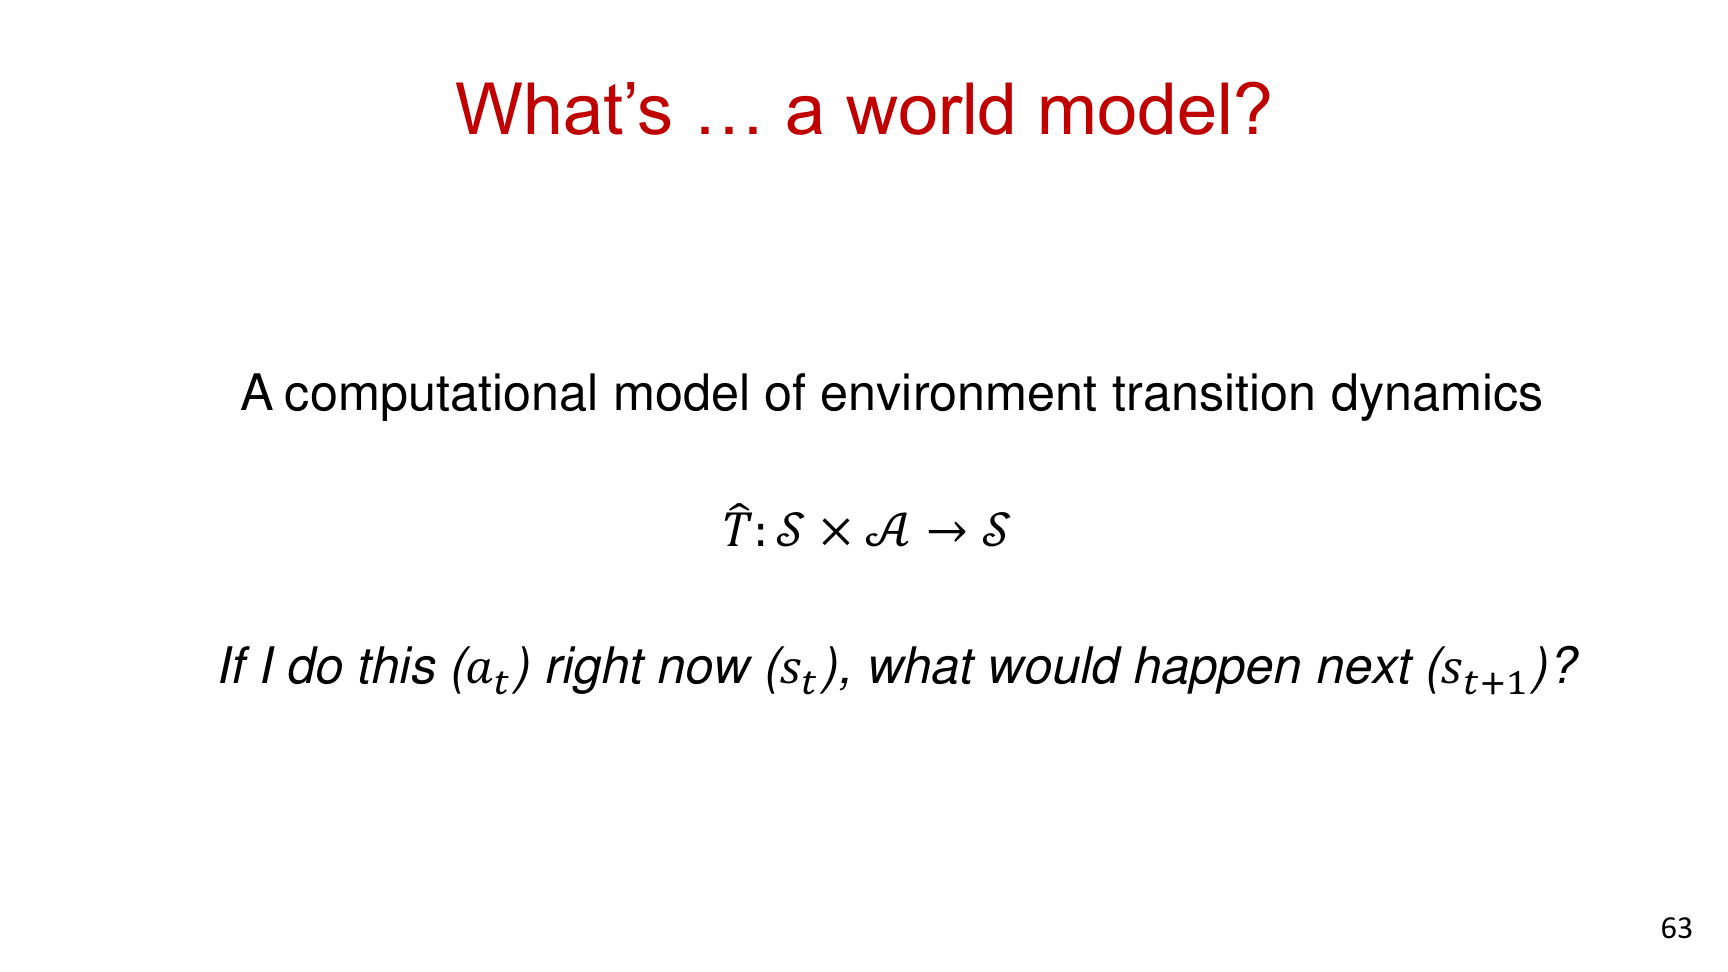
\includegraphics[width=0.74\textwidth]{../lectures/lec03_reasoning_memory_planning/figures/lec03_fig_012.png}
\caption{World model 的最小抽象：在执行动作前先预测状态转移。}
\end{figure}

\begin{figure}[H]
\centering
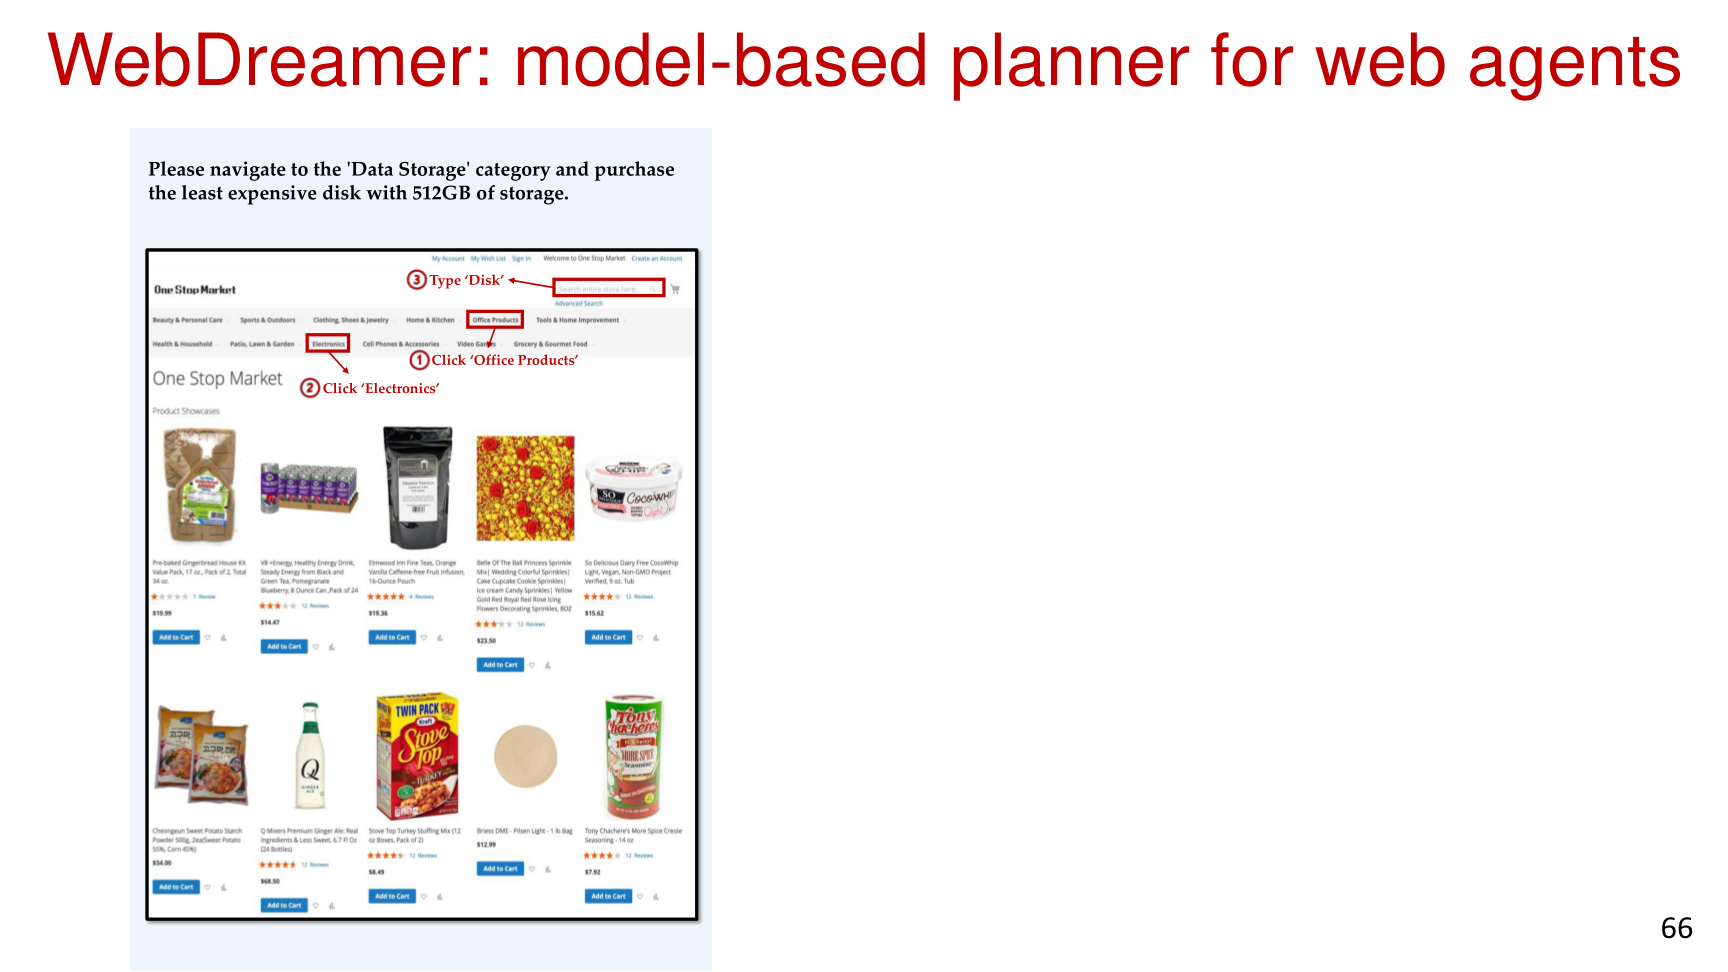
\includegraphics[width=0.78\textwidth]{../lectures/lec03_reasoning_memory_planning/figures/lec03_fig_013.png}
\caption{WebDreamer 的示例：agent 先在内部模拟网页跳转和后续选项，再决定是否真的点击。}
\end{figure}

\begin{lstlisting}
Observe the current webpage state s_t
Enumerate candidate actions
Predict successor states with the world model
Score predicted states with a value function
Execute the best action in the real environment
\end{lstlisting}

\paragraph{为什么这比 reactive planning 更像“高级 agent”}
因为 agent 不再只凭当前页面做局部反应，而是把语言模型用作 environment simulator。它先在内部世界里想象未来，再决定是否把动作提交给外部世界。这与人类 planning 的基本直觉非常接近。

\paragraph{为什么这比 tree search 更现实}
Tree search 假设你可以大量试错；WebDreamer 假设现实里试错有代价，因此应该把更多搜索移入 learned world model。这正是 language agent planning 与纯 benchmark search 的关键区别。

\section{整合视角：memory、reasoning、planning 为什么必须一起看}

\begin{figure}[H]
\centering
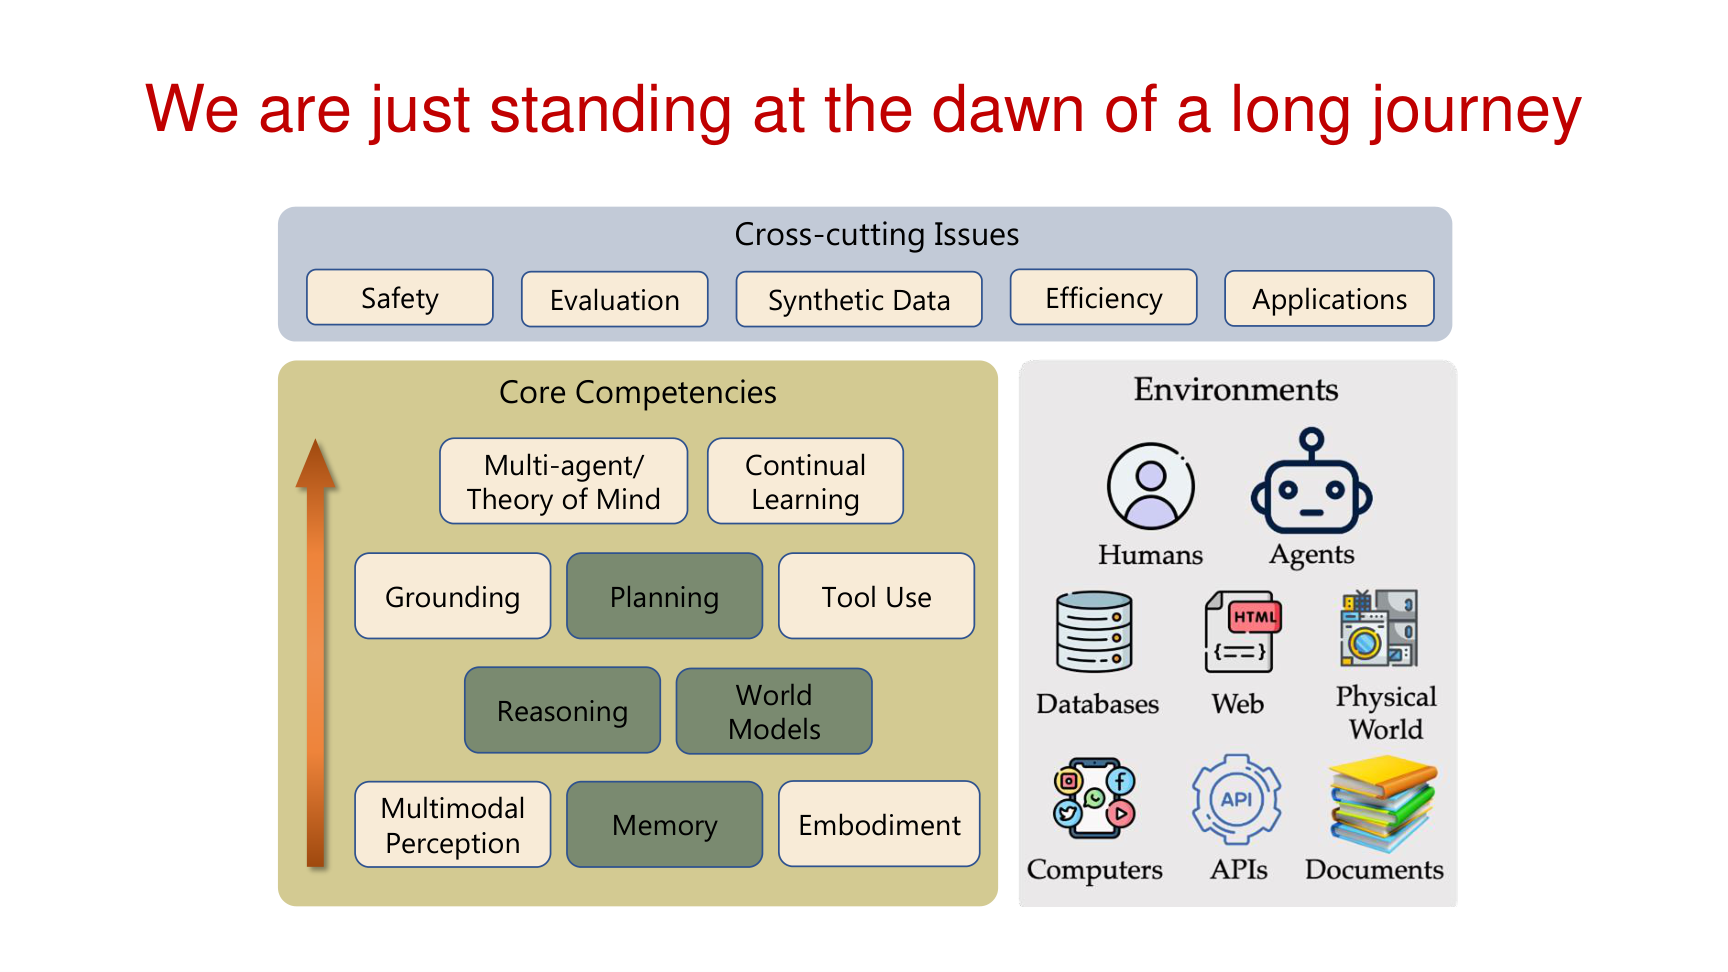
\includegraphics[width=0.82\textwidth]{../lectures/lec03_reasoning_memory_planning/figures/lec03_fig_014.png}
\caption{语言 agent 能力地图：memory、reasoning、world models、planning、grounding、tool use、continual learning 共同构成系统能力。}
\end{figure}

Yu Su 在结尾最重要的贡献，是把 memory、reasoning、planning 重新组织成一个统一能力版图：
\begin{itemize}
\item \textbf{Memory} 决定 agent 能否跨时空整合经验。
\item \textbf{Reasoning} 决定 agent 能否形成和操作抽象状态。
\item \textbf{Planning / World Models} 决定 agent 能否在执行前进行 simulation 与 deliberation。
\end{itemize}

这三者并不是相互独立的。没有 memory，planning 会失忆；没有 reasoning，memory 只剩检索；没有 world model，reasoning 无法稳健转化为行动策略。

\begin{figure}[H]
\centering
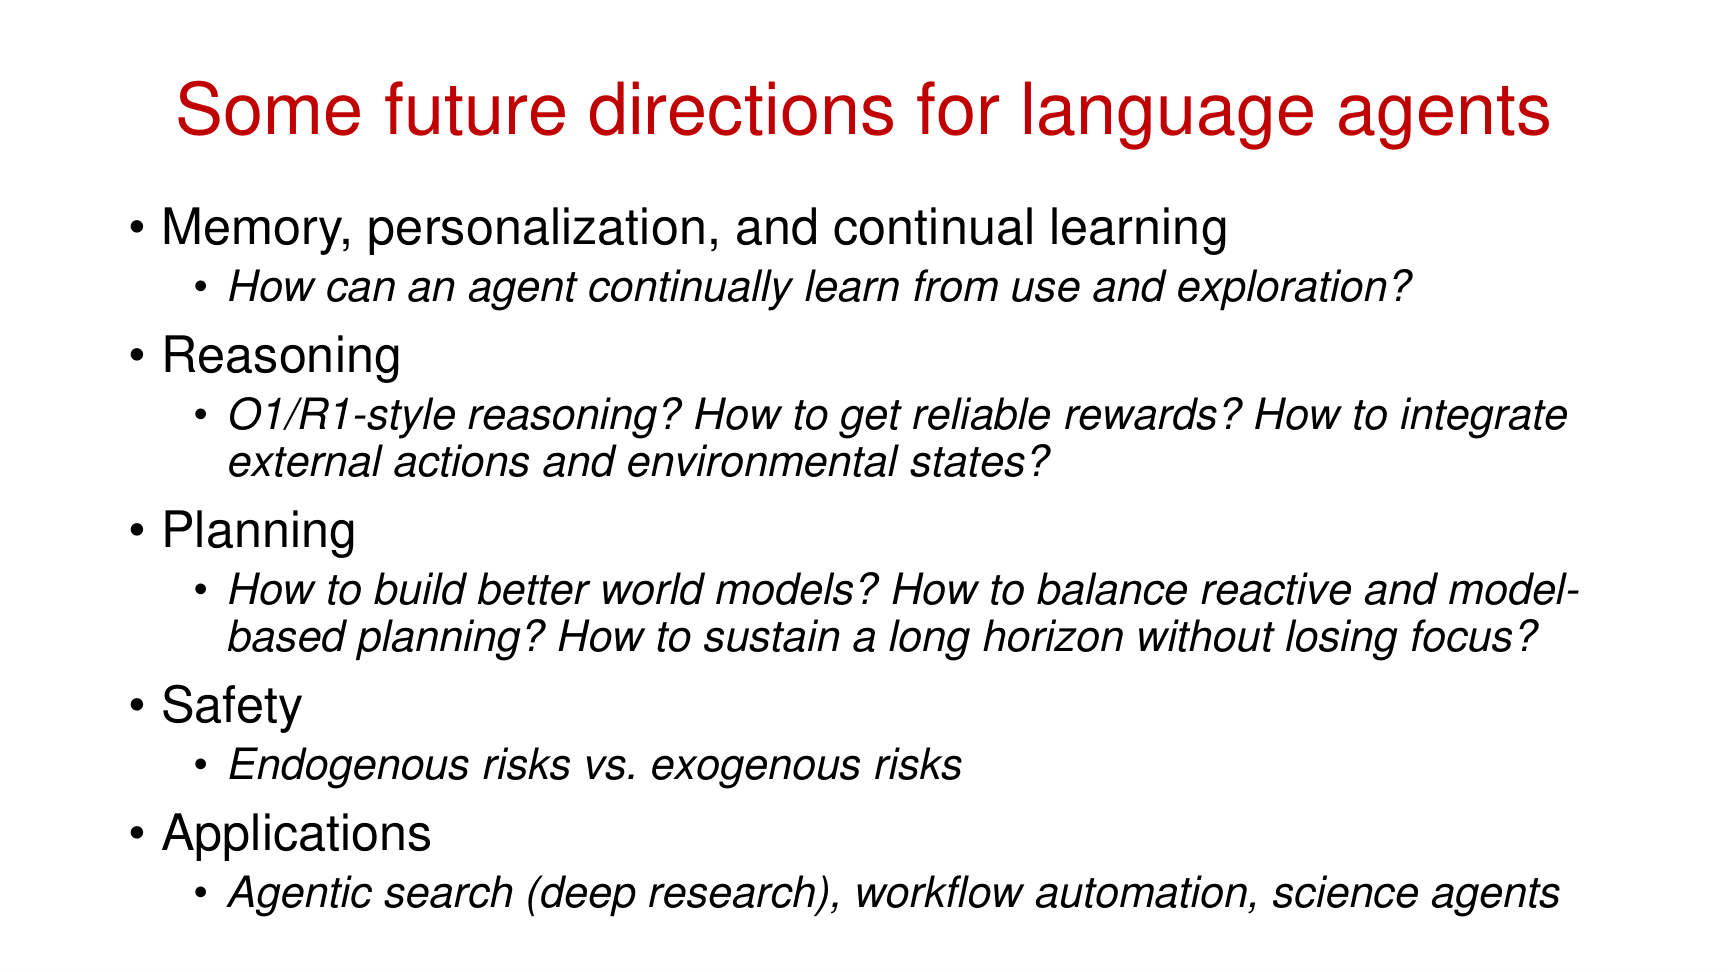
\includegraphics[width=0.80\textwidth]{../lectures/lec03_reasoning_memory_planning/figures/lec03_fig_015.png}
\caption{未来方向页：个性化记忆、持续学习、可靠 reasoning reward、grounding 和规划将共同定义下一代 language agents。}
\end{figure}

\section{与 readings 的连接}

\subsection{HippoRAG：记忆不是外挂，而是结构能力}

HippoRAG reading 让本讲的记忆部分有了非常清晰的技术落点。它说明长期记忆不是“有没有更多文档”，而是“agent 是否有足够好的记忆索引与联想机制”。对自学者来说，这个 reading 也是理解为什么 current RAG 不足以支撑真正 agent memory 的最好入口。

\subsection{Grokked Transformers：显式与隐式推理必须一起讨论}

Grokked Transformers reading 的价值，在于它把隐式推理从抽象命题变成了可分析的电路问题。它提醒我们：对 language agents 来说，显式 CoT 只是接口层；更深层的 reasoning 能力还取决于模型内部能否学到 generalizing circuits。

\subsection{WebDreamer：规划的成本结构发生了变化}

WebDreamer reading 则把 planning 讨论从“会不会 search”推进到“什么时候该在内部 world model 中 search，什么时候才去真实环境执行”。这对 web / GUI / OS agents 尤其关键，因为环境交互有成本且可能不可逆。

\section{失败模式与前后讲联系}

\subsection{本讲最重要的失败模式}

\begin{enumerate}
\item \textbf{把 agent 只当成 workflow wrapper。} 这样会看不到 memory、reasoning、planning 的结构问题。
\item \textbf{把 RAG 当成长期记忆的完整答案。} 浅层检索无法替代联想与索引机制。
\item \textbf{把 CoT 当成全部推理。} 没有 implicit reasoning substrate，再多 verbal thoughts 也可能只是表演。
\item \textbf{在真实环境中过度依赖在线 tree search。} 成本、不可逆性和安全风险会迅速失控。
\item \textbf{把 world model 想象成完美模拟器。} 如果预测误差太大，model-based planning 反而会系统性误导行动。
\end{enumerate}

\subsection{与前后讲的联系}

前两讲主要讨论 reasoning 本身：第一讲关注 inference-time search，第二讲关注 training-time judge。Yu Su 这讲把视角放大到完整 language agent：reasoning 不再只是生成思维链，而是与 memory organization 和 world-model planning 一起构成 agent intelligence。后续 multimodal、theorem proving、安全与抽象发现等讲次，其实都能放进这个框架里继续展开。

\section{本章小结}

如果把本讲压缩成一句话，就是：
\begin{center}
\emph{language agent 的核心不是“会说话”，而是能用语言组织记忆、进行推理、模拟未来并协调行动。}
\end{center}

Yu Su 通过 HippoRAG、Grokked Transformers 和 WebDreamer 给出三条清晰主线：
\begin{itemize}
\item 记忆要从浅层检索升级成结构化联想系统。
\item 推理既有显式外显层，也有隐式参数电路层。
\item 规划要从 reactive execution 走向 model-based deliberation。
\end{itemize}

对整门课而言，这一讲相当于给“advanced LLM agents”补上了系统架构视角：单点优化某个 prompt 或某个 benchmark 技巧远远不够，真正的难点在于如何让 memory、reasoning、planning 在同一 agent 中形成闭环。

\section{复习题}

\begin{enumerate}
\item 为什么 Yu Su 坚持使用 “language agent” 而不是泛泛的 AI agent？
\item 当前 RAG 在多跳记忆问题上的主要缺陷是什么？
\item HippoRAG 为什么要用图结构和 Personalized PageRank，而不是只做 dense retrieval？
\item Grokking 为什么说明 implicit reasoning 与 generalization 有深层联系？
\item WebDreamer 与 reactive web agent 的最关键区别是什么？
\end{enumerate}

\section{深入思考题}

\begin{enumerate}
\item 如果 world model 预测常常不准，agent 应该如何在真实环境反馈与内部模拟之间做校准？
\item 对长期个性化 agent 来说，memory retrieval、memory editing 与 privacy control 应该如何共同设计？
\item 你是否认同“显式 CoT 只是 reasoning 的接口层”这个判断？请结合 agent system 设计给出论证。
\end{enumerate}

\section{延伸阅读}

\begin{itemize}
\item \textbf{HippoRAG}：理解长期记忆为何需要索引与联想机制。
\item \textbf{Grokked Transformers}：理解 implicit reasoning 的学习与泛化机制。
\item \textbf{WebDreamer}：理解真实环境 planning 为什么要依赖 world models。
\item 配合本门课后续 multimodal agent、GUI agent 与 formal reasoning 章节一起阅读，可以更清晰地看到 language agent 能力地图如何向多模态、可验证和安全方向扩展。
\end{itemize}

\part{Agentic Workflows, Tools, and Code}
\chapter{Open Training Recipes for Reasoning in Language Models}
\label{chap:lec04_open_training_recipes_reasoning}
\section{本讲学习目标}
\begin{itemize}
\item 理解为什么开放生态与可复现 recipe 是 reasoning 研究的前提条件。
\item 分清楚 SFT、preference tuning、RLVR 与 test-time scaling 的职责边界。
\item 看懂 DPO 与 PPO 的关系，以及为什么 data quality 往往比算法标签更重要。
\item 理解 s1 / s1K / budget forcing 如何把训练阶段与测试时推理衔接起来。
\end{itemize}

\section{背景与问题设置}
\subsection{为什么本讲先讲 open recipe，而不是直接讲一个 reasoning 技巧}
Hanna Hajishirzi 一开始就把话题放在 open ecosystem 上，这不是铺垫，而是 lecture 的方法论中心。她的核心论点是：当训练数据、权重、配方、评估和工具链无法被研究者检查时，很多所谓的 “best practices” 其实无法真正变成科学知识。对 reasoning model 尤其如此，因为我们讨论的不是单一 prompt trick，而是一条跨越预训练、后训练和测试时计算分配的工艺链。

\begin{figure}[H]
\centering
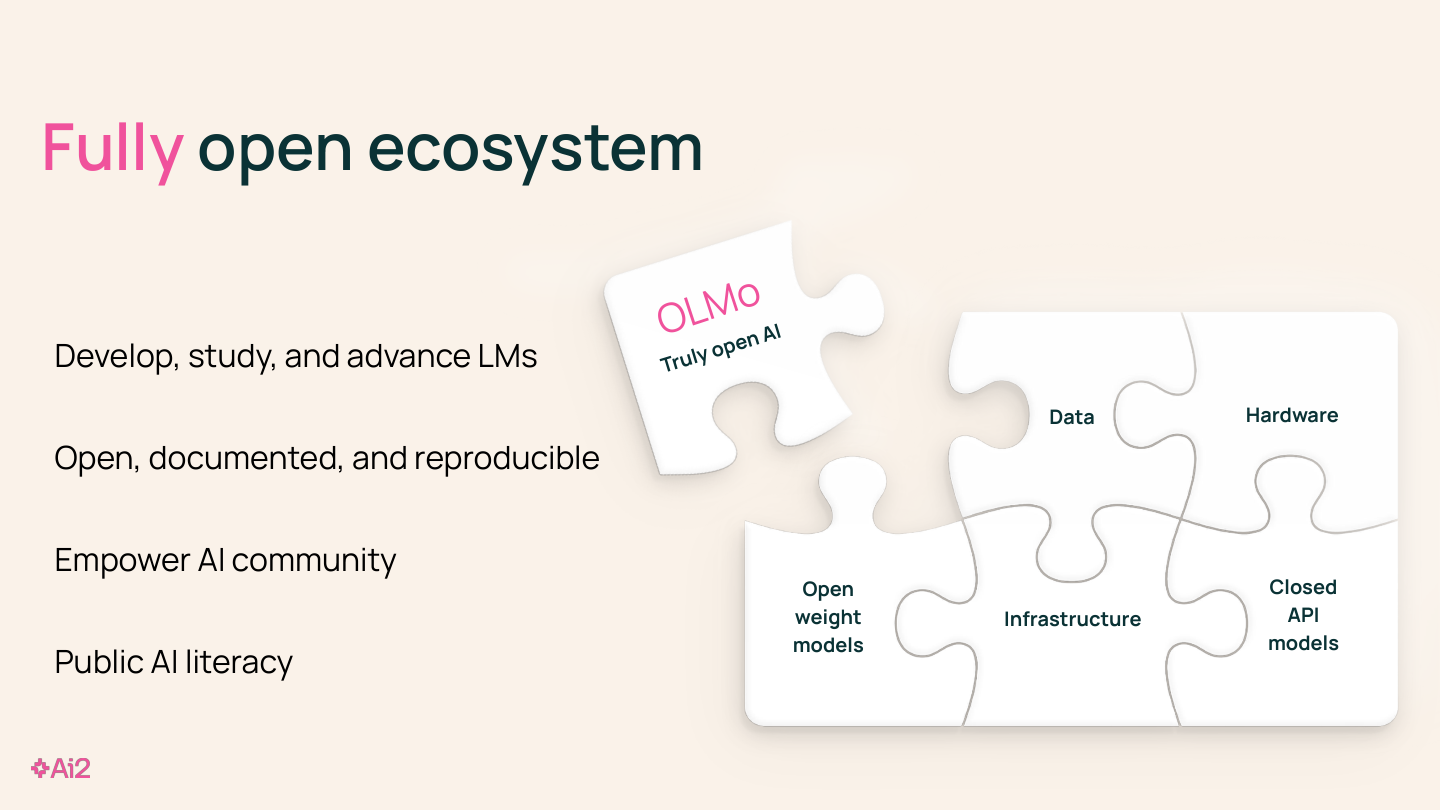
\includegraphics[width=0.82\textwidth]{../lectures/lec04_open_training_recipes_reasoning/figures/lec04_fig_001.png}
\caption{开放语言模型生态图：开放数据、开放工具、开放权重与开放基础设施一起决定 recipe 能否被复做。}
\end{figure}

Slides 对 fully open 的要求也讲得非常明确：不仅要开放模型权重，还要尽可能让训练过程透明、让他人可以访问、复现并质疑数据与配方。这个要求和 agent 课程的关系非常直接：如果你想比较不同 reasoning recipe 的效果，没有可复现的 evaluator 和配方，你根本无法知道性能变化来自哪里。

\begin{figure}[H]
\centering
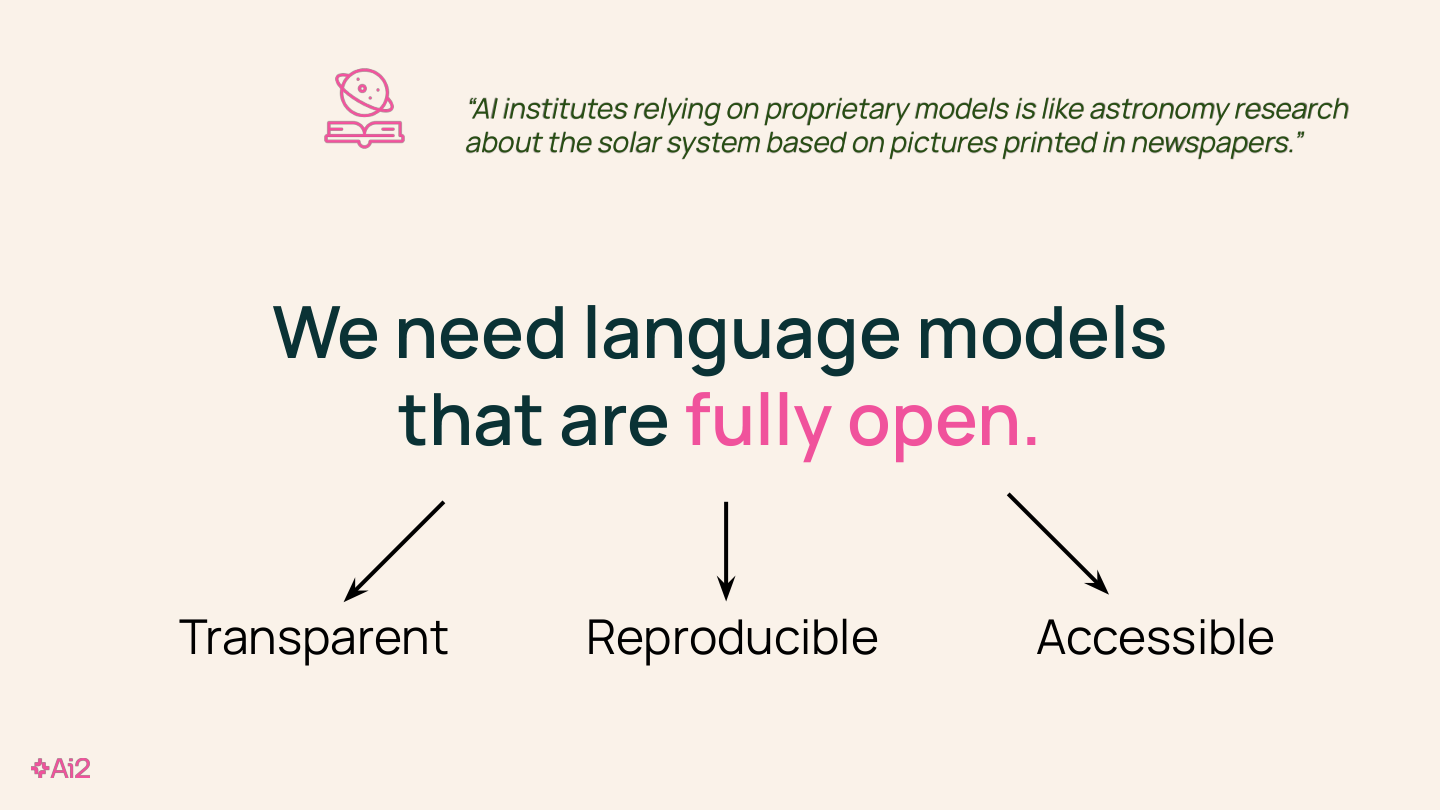
\includegraphics[width=0.76\textwidth]{../lectures/lec04_open_training_recipes_reasoning/figures/lec04_fig_002.png}
\caption{本讲对 fully open 的要求：transparent、reproducible、accessible。}
\end{figure}

\begin{knowledgebox}{本讲的统一视角}
本讲把 reasoning 训练看成一条 staged recipe：先准备 base model，再用不同监督信号逐层塑形，最后在 inference time 把额外预算投到最值得扩展的推理步骤上。
\end{knowledgebox}

\subsection{预训练、后训练与测试时推理的三段式视角}
Slides 第 9--10 页把整个问题拆成三个阶段：pre-training、post-training、test-time inference。这个拆法看似简单，但它避免了一个常见误区：把 reasoning 只当成部署时的 prompt engineering。Hajishirzi 的意思是，想要稳定的 reasoning 行为，训练与测试时必须协同设计。

\begin{figure}[H]
\centering
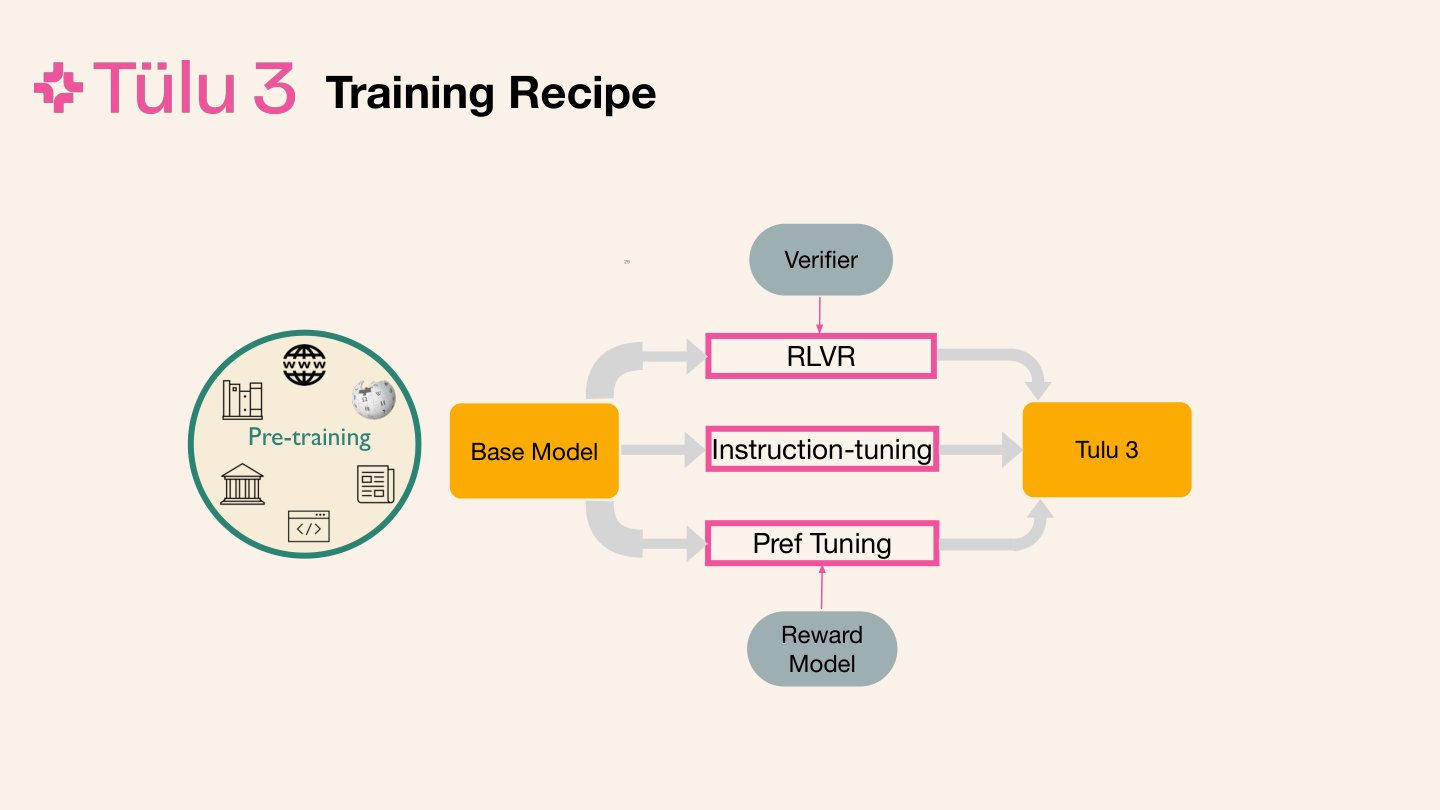
\includegraphics[width=0.83\textwidth]{../lectures/lec04_open_training_recipes_reasoning/figures/lec04_fig_003.png}
\caption{Tulu 3 的阶段化 recipe：base model 之后，按 instruction tuning、preference tuning、RLVR 等阶段逐步增强能力。}
\end{figure}

在这套视角中，监督微调负责把模型从“会续写”变成“会按任务格式做事”；preference tuning 负责把输出风格和偏好对齐；RLVR 负责在存在可验证答案的任务上进一步放大 reasoning 正确率；test-time scaling 则负责在部署时继续把预算换成更高质量的推理轨迹。

\[
\mathcal{L}_{\mathrm{SFT}}(\theta) = -\sum_{(x,y) \in \mathcal{D}_{\mathrm{inst}}} \sum_{t=1}^{|y|} \log p_{\theta}(y_t \mid x, y_{<t})
\]

上式是 lecture 中 supervised finetuning 的数学化抽象。Slides 虽然没有写出完整公式，但它讲的本质就是：给定 instruction-response 配对数据，最大化目标回答的条件概率。这里每个符号的含义分别是：$\mathcal{D}_{\mathrm{inst}}$ 表示 instruction 数据集，$x$ 是 prompt，$y$ 是期望输出，$p_{\theta}$ 是当前策略模型。

\section{监督微调与数据 recipe}
\subsection{SFT 的难点不是目标函数，而是数据从哪里来}
Lecture 对 SFT 的讲法很克制。Hajishirzi 没有把重点放在损失函数，而是强调 data curation, data mixing 和 quality control。因为 instruction tuning 最大的难点不是优化器，而是你到底拿什么数据把模型往哪个能力方向推。

\begin{figure}[H]
\centering
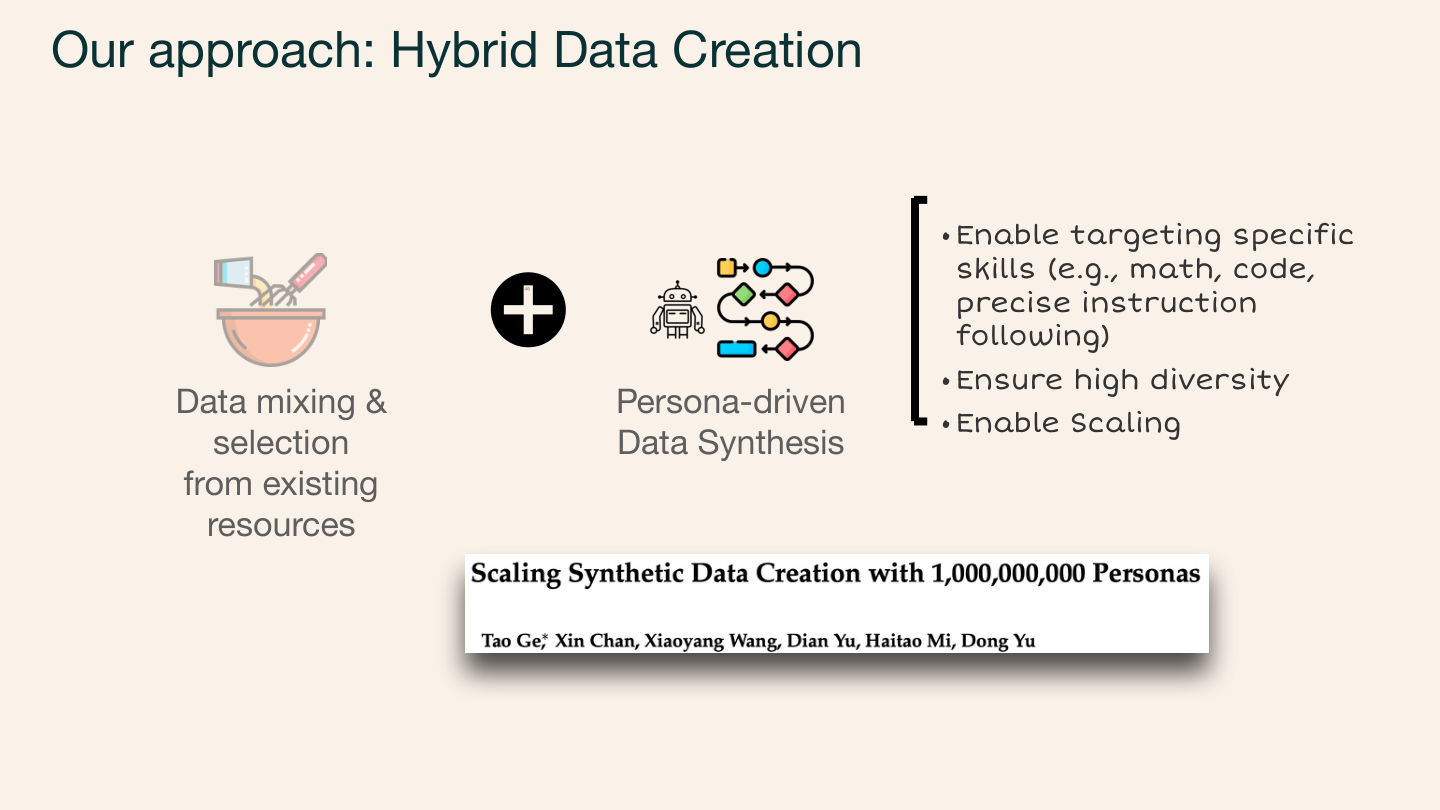
\includegraphics[width=0.82\textwidth]{../lectures/lec04_open_training_recipes_reasoning/figures/lec04_fig_004.png}
\caption{Persona-driven data creation：通过 persona 与目标能力来控制 synthetic reasoning/coding/instruction-following 数据。}
\end{figure}

Slides 连续展示了 Self-Instruct、公开 instruction datasets、hybrid preferences、persona-driven data synthesis 等材料。它们的共同点是：都在尝试用更便宜、更可扩展的方式补齐昂贵的人类标注。尤其是 persona-driven synthesis，它的价值不在于 “合成数据越多越好”，而在于你可以按 math、coding、precise instruction following 等目标能力来有控制地生成数据。

\begin{figure}[H]
\centering
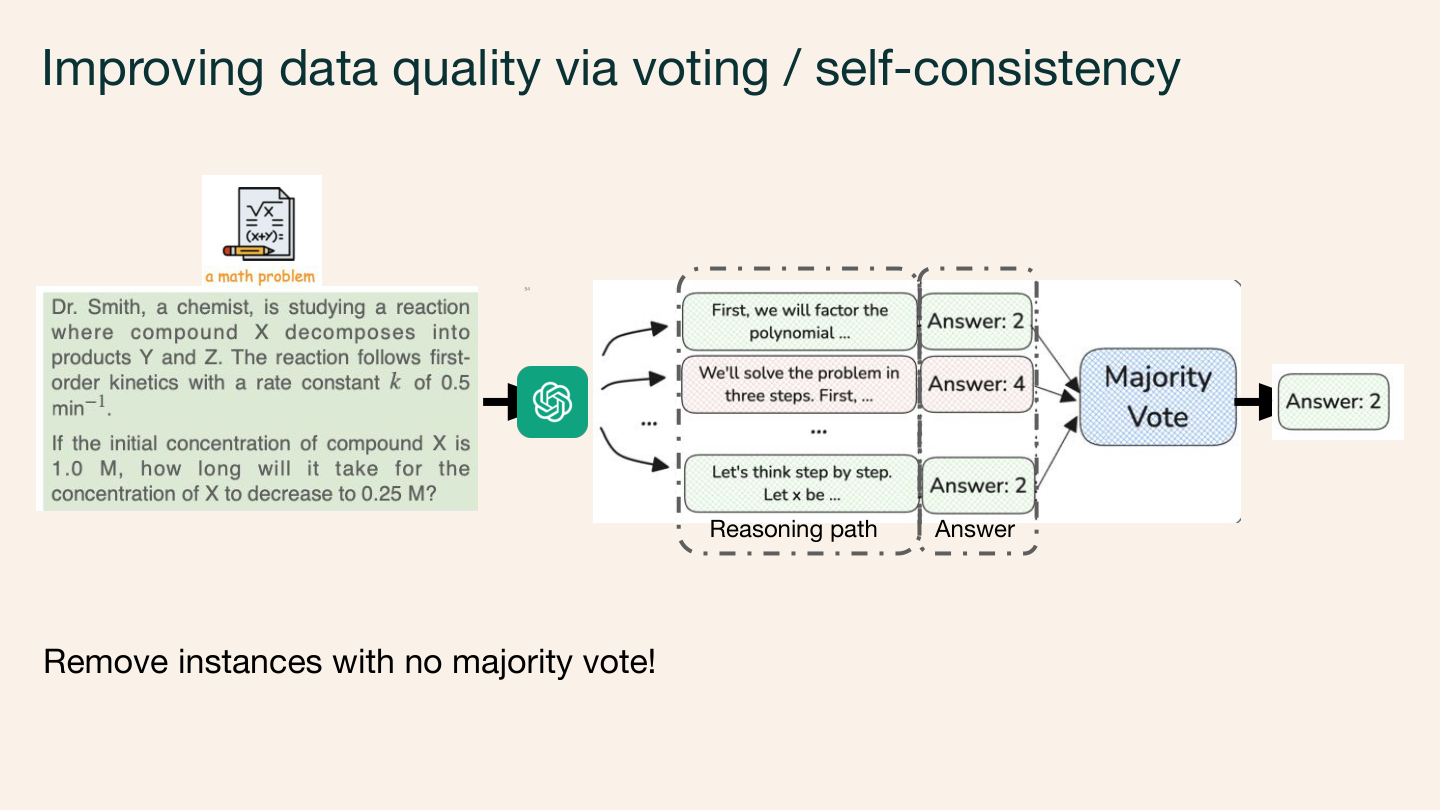
\includegraphics[width=0.75\textwidth]{../lectures/lec04_open_training_recipes_reasoning/figures/lec04_fig_005.png}
\caption{Voting / self-consistency 过滤 reasoning 数据：先用便宜的自动信号筛掉明显不可靠的 traces。}
\end{figure}

这里有一个非常实用的 recipe 观点：reasoning 数据不只是 final answer，更重要的是 reasoning trace 本身。Chain-of-thought 数据有三重作用。第一，它让模型学习多步问题的展开方式；第二，它把错误暴露在中间步骤上；第三，它使数据筛选成为可能，例如通过 voting / self-consistency 保留较可信的样本。

\begin{lstlisting}
capabilities = ['chat', 'knowledge', 'reasoning', 'coding', 'safety']
for cap in capabilities:
    pool = curate_sources(cap)
    filtered = filter_low_quality(pool)
    mixture.extend(sample_with_budget(filtered, target=cap))
\end{lstlisting}

这段伪代码体现的是 lecture 的真正工程逻辑：先定义能力类别，再分别收集、过滤、采样，而不是把一切数据丢进一个大桶里训练。

\begin{importantbox}{为什么朴素地“多收一点数据”不够}
Slides 反复强调许可证检查、去污染（decontamination）、目标能力驱动的 evaluator，以及 mixture balancing。没有这些步骤，更多数据很可能只是更多噪声，甚至会让 reasoning 能力和安全能力互相干扰。
\end{importantbox}

\subsection{Tulu 3 reading 如何补全 lecture 中的 recipe 细节}
《Tulu 3》把 lecture 中的经验写成了论文级 recipe。它最有价值的地方不是某个单一技术点，而是清楚展示了 open post-training 需要哪些材料同时开源：数据、代码、训练脚本、评测、模型以及中间设计权衡。lecture 本身更多讲“怎么想”，而 reading 给出了“怎么复做”。

\section{Preference tuning：DPO 与 PPO 的边界}
Slides 在第 66--78 页把 RLHF 结构拆得非常清楚：prompt 进入 policy，得到多个 response；人类或 AI feedback 形成 preference data；然后你可以训练 reward model，再做 PPO，或者走 DPO 这条更直接的路。

\begin{figure}[H]
\centering
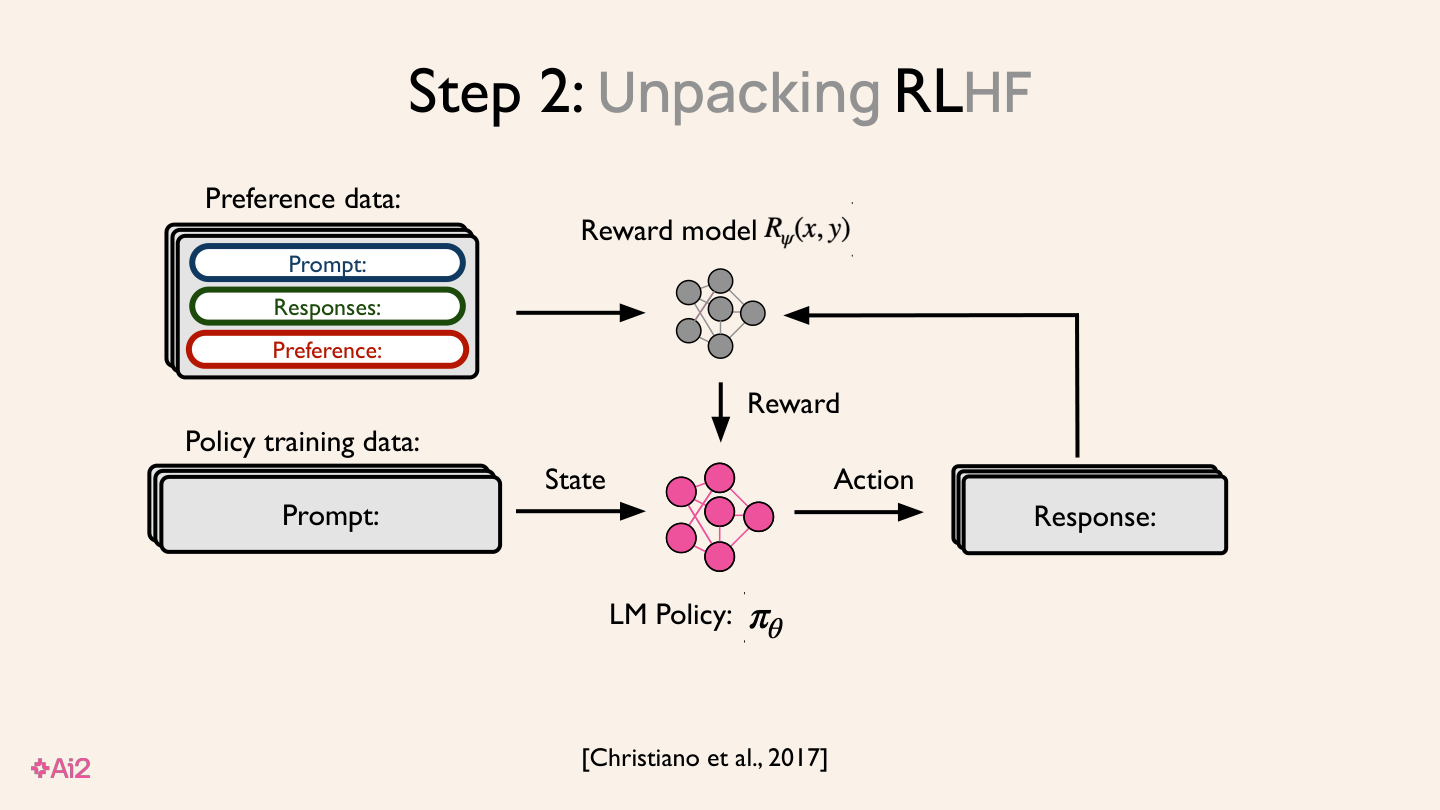
\includegraphics[width=0.84\textwidth]{../lectures/lec04_open_training_recipes_reasoning/figures/lec04_fig_006.png}
\caption{RLHF 组件分解图：preference learning 本质上是在 prompts、responses、reward model 与 policy optimization 之间组织监督信号。}
\end{figure}

\[
\max_{\pi_\theta} \ \mathbb{E}_{x, y \sim \pi_\theta}[r_\phi(x,y)] - \beta \operatorname{KL}(\pi_\theta(\cdot \mid x) \| \pi_{\mathrm{ref}}(\cdot \mid x))
\]

这个 KL-regularized objective 对应 lecture 中 “不要离 base model 太远” 的直觉。$r_{\phi}$ 是 reward model，$\pi_{\theta}$ 是当前 policy，$\pi_{\mathrm{ref}}$ 是 reference model，$\beta$ 控制偏离 reference model 的代价。

\[
\mathcal{L}_{\mathrm{DPO}}(\theta) = -\log \sigma\left(\beta \left[\log \frac{\pi_\theta(y^+\mid x)}{\pi_{\mathrm{ref}}(y^+\mid x)} - \log \frac{\pi_\theta(y^-\mid x)}{\pi_{\mathrm{ref}}(y^-\mid x)}\right]\right)
\]

DPO 的关键在于：不用显式训练 reward model 也能直接利用 preference pairs。这里 $y^+$ 与 $y^-$ 分别表示偏好较好与较差的回答。DPO 的吸引力是实现简单、吞吐高、很适合快速实验；但 lecture 也明确给出工程判断：PPO 通常还能再涨一点，只是更贵、更复杂。

\begin{figure}[H]
\centering
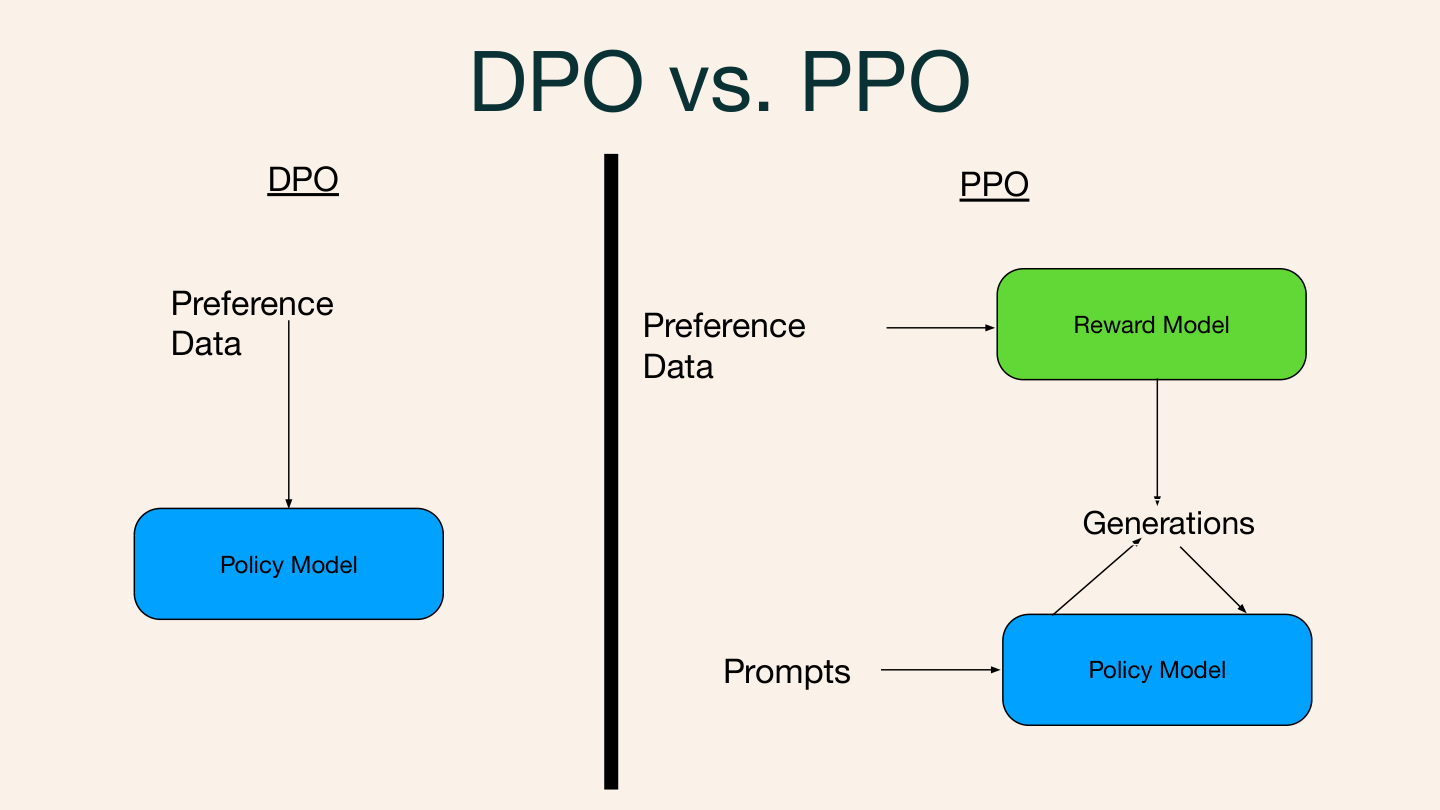
\includegraphics[width=0.78\textwidth]{../lectures/lec04_open_training_recipes_reasoning/figures/lec04_fig_007.png}
\caption{DPO 与 PPO 的训练路径对比。lecture 的重点不是站队，而是理解哪个环节在当前 recipe 中最可能成为瓶颈。}
\end{figure}

\begin{lstlisting}
pairs = collect_preferences(prompts, responses)
if algorithm == 'DPO':
    train_policy_on_pairs(pairs, ref_model)
else:
    reward_model = fit_reward_model(pairs)
    ppo_train(policy, reward_model, prompts)
\end{lstlisting}

《Unpacking DPO and PPO》对这部分的补充很关键。它告诉我们：better preference data 往往比算法标签更重要；更大的 reward model 也不一定自动带来更好的 downstream assistant；policy-training prompts 也有实际影响。换句话说，preference tuning 是系统工程，不是名词工程。

\section{RLVR：在可验证任务上把 reasoning 训练成 RL 问题}
Lecture 在第 97--118 页转向 reinforcement learning with verifiable rewards。这里的关键条件是：任务必须存在可以自动检验的最终答案或约束，例如数学题、可核验 instruction following 或其他 rule-based correctness criterion。

\begin{figure}[H]
\centering
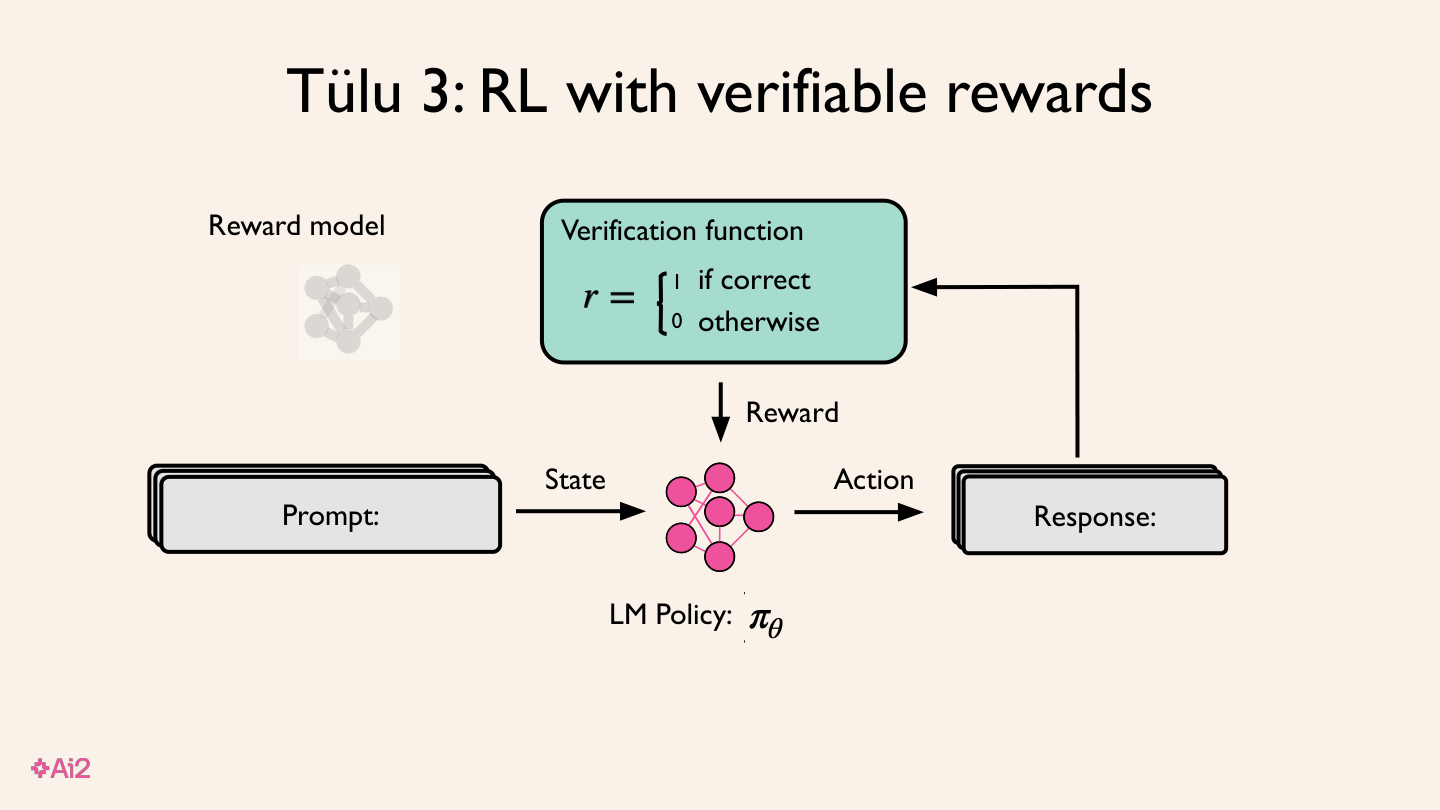
\includegraphics[width=0.8\textwidth]{../lectures/lec04_open_training_recipes_reasoning/figures/lec04_fig_008.png}
\caption{RLVR 的核心结构：不再拟合 reward model，而是直接用 verification function 对最终答案打二值或稀疏奖励。}
\end{figure}

\[
r(x,y) = \mathbf{1}[V(x,y)=1], \qquad \max_{\pi_\theta} \mathbb{E}_{x, y \sim \pi_\theta}[r(x,y)]
\]

这条公式很重要。$V(x,y)$ 是 verification function，检查给定 prompt $x$ 和回答 $y$ 是否满足 gold answer 或规则约束；一旦可验证，奖励 $r(x,y)$ 就可以写成简单的指示函数。这解释了为什么 RLVR 在 reasoning 任务上会突然变得实用：它不需要人类去标每一步 chain-of-thought，只要最终答案可检验即可。

\begin{lstlisting}
for prompt in verifier_dataset:
    answer = policy.sample(prompt)
    reward = verifier(prompt, answer)
    policy = ppo_update(policy, prompt, answer, reward)
\end{lstlisting}

但 lecture 也明确指出了边界：RLVR 更适合 final answer 可验证的任务，不适合开放域聊天；奖励稀疏意味着优化很容易不稳定；而且它未必会学出“优雅”的 reasoning，只会学出“更容易通过 verifier”的策略。因此 verifier 设计、训练集选择和过优化风险非常关键。

\section{s1、budget forcing 与最小 reasoning recipe}
Lecture 最值得和第一讲连起来读的部分，是第 124--142 页关于 s1 的讨论。Hajishirzi 展示了一种令人印象深刻的最小 recipe：只用相对少量但高质量、困难且多样的 reasoning 样本 s1K，再配一个非常简单的 test-time scaling 方法 budget forcing，就可以得到明显的 reasoning 增益。

\begin{figure}[H]
\centering
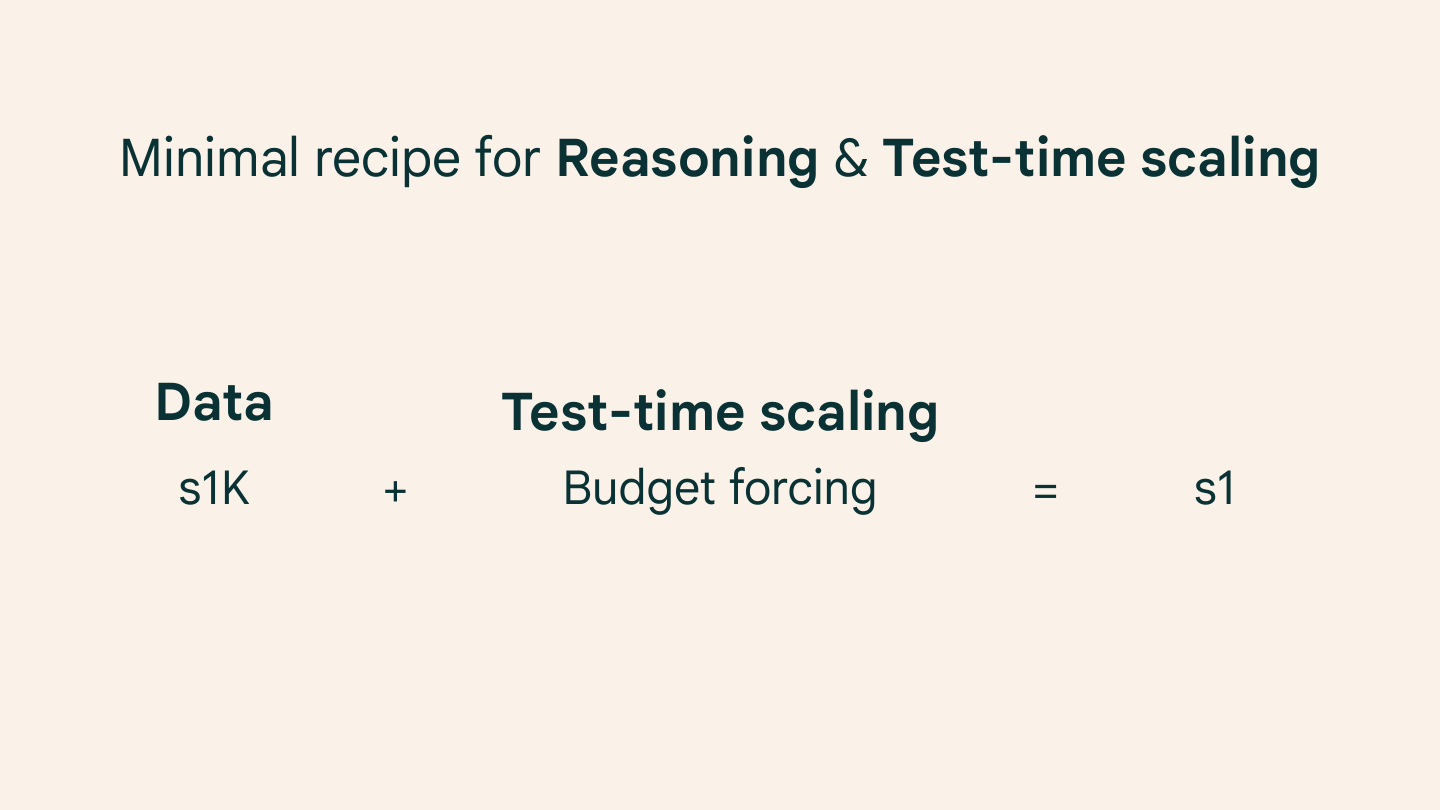
\includegraphics[width=0.79\textwidth]{../lectures/lec04_open_training_recipes_reasoning/figures/lec04_fig_009.png}
\caption{s1 的最小 recipe：高质量 reasoning data 加简单但有效的 budget forcing。}
\end{figure}

\[
y = \operatorname{Decode}(x; B), \qquad B' > B \Rightarrow \text{allow additional reasoning steps or forced continuation tokens}
\]

这个抽象表达的不是某个唯一实现，而是 lecture 的核心思想：你可以显式控制推理预算 $B$，并通过更大的预算 $B'$ 允许更多 reasoning steps，甚至强制继续生成思考过程。Slides 里的 budget forcing 例子之所以重要，在于它说明 reasoning gain 不一定要靠更大模型或更多训练 token，也可以来自更聪明的 test-time compute allocation。

\begin{lstlisting}
answer = policy.generate(prompt, max_tokens=budget)
while not stop(answer) and spent(answer) < forced_budget:
    answer += policy.generate('Wait', continue_from=answer)
\end{lstlisting}

\begin{figure}[H]
\centering
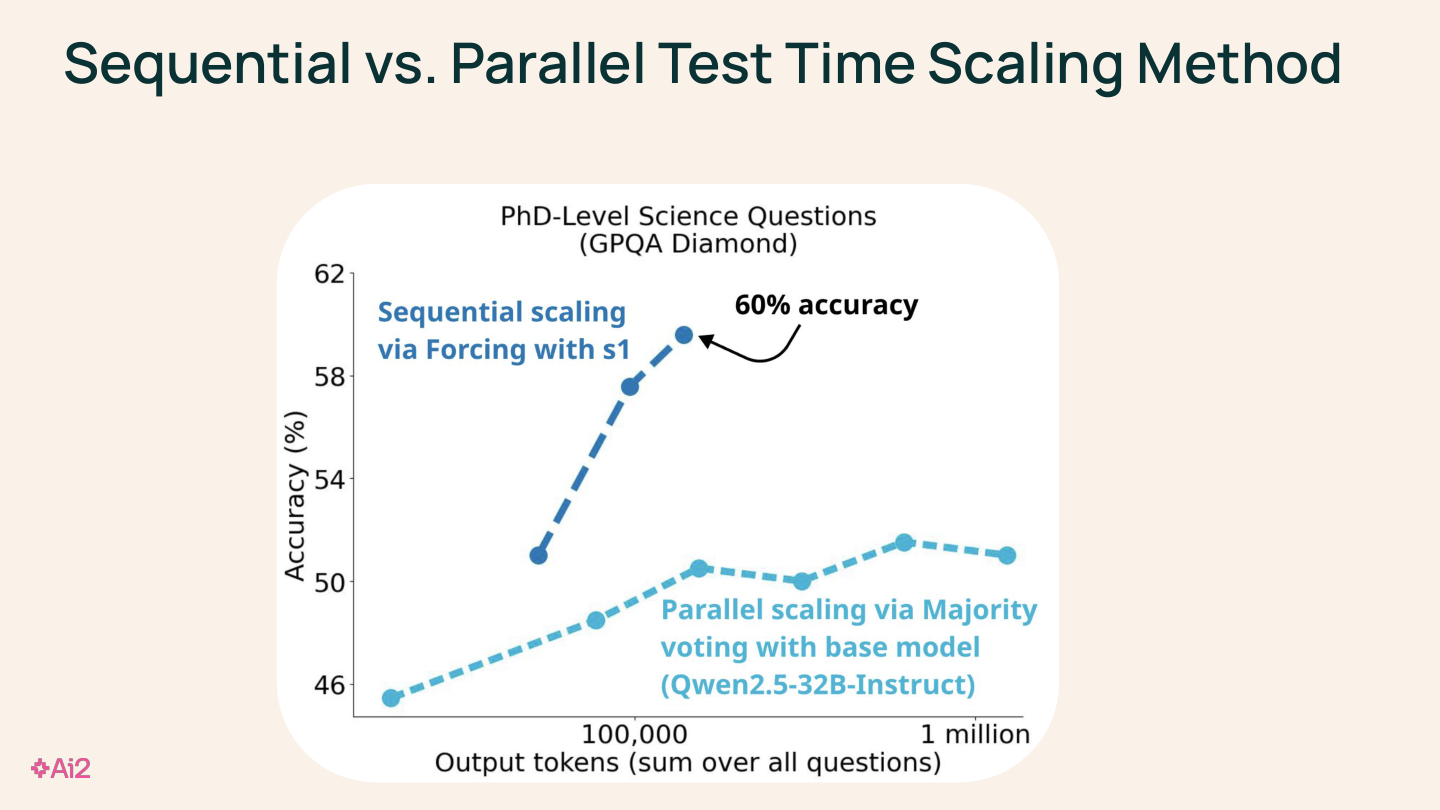
\includegraphics[width=0.82\textwidth]{../lectures/lec04_open_training_recipes_reasoning/figures/lec04_fig_010.png}
\caption{Sequential 与 parallel test-time scaling 的区别：预算可以投在延长单条轨迹，也可以投在扩展候选空间。}
\end{figure}

这一段与第一讲的 inference-time techniques 正好形成闭环：L01 讨论“怎么花 test-time compute”；L04 讨论“训练 recipe 怎样为这种花法做准备”。没有合适的训练数据和 staged post-training，单纯延长思考很可能只会延长错误轨迹。

\section{与关键 readings、前后讲和失败模式的联系}

\subsection{Tulu 3：为什么“开放 recipe”不能只开 checkpoint}

《Tulu 3》是本讲最核心的 reading，因为 lecture 中反复强调的 staged recipe 基本都能在这篇 paper 里找到对应物。它真正说明的是：所谓 open post-training，不是把一个指令模型权重扔出来就结束，而是要把 \textbf{阶段顺序、数据治理、评测方式和复现实践} 一并公开。否则社区只能看到结果，看不到为什么这个结果能成立。

这也解释了 slides 中为何反复出现 data mixture、stage ordering 和 evaluator choice。Tulu 3 的 strongest claim 不是“公开模型也能强”，而是“当 SFT、preference tuning 与 reasoning-oriented RL 被按合适顺序组织时，公开 recipe 可以逼近甚至超过很多强 instruct baseline”。但它同样保留了一个重要限制：\textbf{上游 base model 的能力边界仍然存在}。如果 base model 的长程 reasoning basis 很弱，后面的 recipe 只能局部修正，而很难凭空创造能力。

\subsection{Unpacking DPO and PPO：lecture 的工程判断为什么成立}

《Unpacking DPO and PPO》让本讲对 DPO/PPO 的立场更具体。lecture 并没有说“算法不重要”，而是说\textbf{如果 preference data 和 evaluator 已经不可靠，那么算法名词本身很难救场}。这篇 reading 的系统消融恰好支持这一点：better preference data 往往是最大的杠杆，reward model 规模、policy-training prompt 和学习算法都会影响结果，但它们的作用方式并不等价。

因此 lecture 的工程判断其实有两层。第一层是：PPO 往往还能比 DPO 再涨一点，但代价是更重的实现复杂度、吞吐成本和调参负担。第二层是：对很多开放研究团队而言，\textbf{先把 data quality、prompt construction 和 evaluator 站稳，再比较 DPO/PPO，才是更合理的资源分配顺序}。这也能解释为什么 Hajishirzi 在 slides 里把算法、数据、评测放进同一个 recipe 视角，而不是单独给某个算法封神。

\subsection{OpenScholar：为什么开放基础设施会在下游 agent 中兑现}

《OpenScholar》虽然不是这场 lecture 的主体算法，但它提供了一个非常关键的下游例子：开放模型、开放 retrieval pipeline 和 citation-grounded synthesis 结合后，能够显著降低 citation hallucination。这使它成为 lecture 开头“开放基础设施有技术含义”的直接证据。

更重要的是，它提醒读者：开放 recipe 的价值不止体现在 benchmark leaderboard。真正长期的价值，是它能让 scientific agents、retrieval-augmented assistants 和领域专用系统在 attribution、reproducibility 和 error analysis 上更可控。本讲讲的是 training recipe，而 OpenScholar 展示的是\textbf{这些 recipe 进入下游系统后，会如何改变 agent 的可信度上限}。

本讲最需要警惕的失败模式包括：
\begin{itemize}
\item 把开放误解为只开权重，而忽视数据、配方与评测的可复现性。
\item 把 DPO/PPO 之争当成全部问题，忽视 preference data 与 evaluator 的质量。
\item 在没有可靠 verifier 的任务上生搬硬套 RLVR。
\item 误以为 budget forcing 永远有用，而忽视模型是否已经具备可扩展的 reasoning basis。
\end{itemize}

与前一讲的关系：L01 讲的是 inference-time reasoning methods；本讲解释这些方法为什么需要被训练 recipe 支撑。与下一讲的关系：L05 会把这种 recipe 观念带进 coding agents 和 vulnerability detection，进一步强调 environment feedback 与 verification 的角色。

\section{本章小结}
本讲最重要的教材结论是：reasoning 不是单一阶段的问题，而是贯穿数据、SFT、偏好优化、RL 与 test-time compute allocation 的系统工程。开放 recipe 的价值在于，它让这些决策可以被研究社区真正检验、继承和改进。

\section{复习题}
\begin{itemize}
\item 为什么开放生态在本讲中是技术命题而不只是社区命题？
\item SFT、preference tuning、RLVR 三者在监督信号上有何差别？
\item 为什么 better preference data 往往比 DPO 与 PPO 的标签更重要？
\item RLVR 适用的任务边界是什么？
\item s1 与 budget forcing 如何体现最小 reasoning recipe？
\end{itemize}

\section{深入思考题}
\begin{itemize}
\item 如果你只能做一个阶段改进，你会优先改进 evaluator、data mixture 还是优化算法？为什么？
\item 什么样的 verifier 最容易诱发 reward hacking？如何缓解？
\item 在开放模型研究中，哪些资源最需要被优先开源才能真正支持科学复现？
\end{itemize}

\section{延伸阅读}
\begin{itemize}
\item Tulu 3: Pushing Frontiers in Open Language Model Post-Training
\item Unpacking DPO and PPO: Disentangling Best Practices for Learning from Preference Feedback
\item OpenScholar: Synthesizing Scientific Literature with Retrieval-augmented LMs
\end{itemize}

\chapter{Coding Agents and AI for Vulnerability Detection}
\label{chap:lec05_coding_agents_vulnerability_detection}
\section{本讲学习目标}
\begin{itemize}
\item 理解 coding agent 的定义为何强调多轮工具使用和 environment feedback。
\item 区分 dynamic control 与 procedural control 两类 coding-agent 设计。
\item 理解 security tasks 为什么要求交互式工具、sandbox 和强验证。
\item 看懂 Big Sleep 如何把真实漏洞研究 framing 成 variant analysis workflow。
\end{itemize}

\section{为什么 evaluator 先于 architecture}
Sutton 开头最重要的技术观点，其实不是某个 agent loop，而是 evaluator 决定设计。早期代码生成 benchmark 如 HumanEval 和 MBPP 强调 pass@k：给定 prompt，采样若干程序，看其中是否有正确答案。这类 evaluator 在 2021 年非常有用，因为难度适中、不易泄漏、能推动模型进步；但到 2025 年，它们已经太容易、测试用例太少、泄漏也太严重，很难再指导 agent 设计。

\begin{figure}[H]
\centering
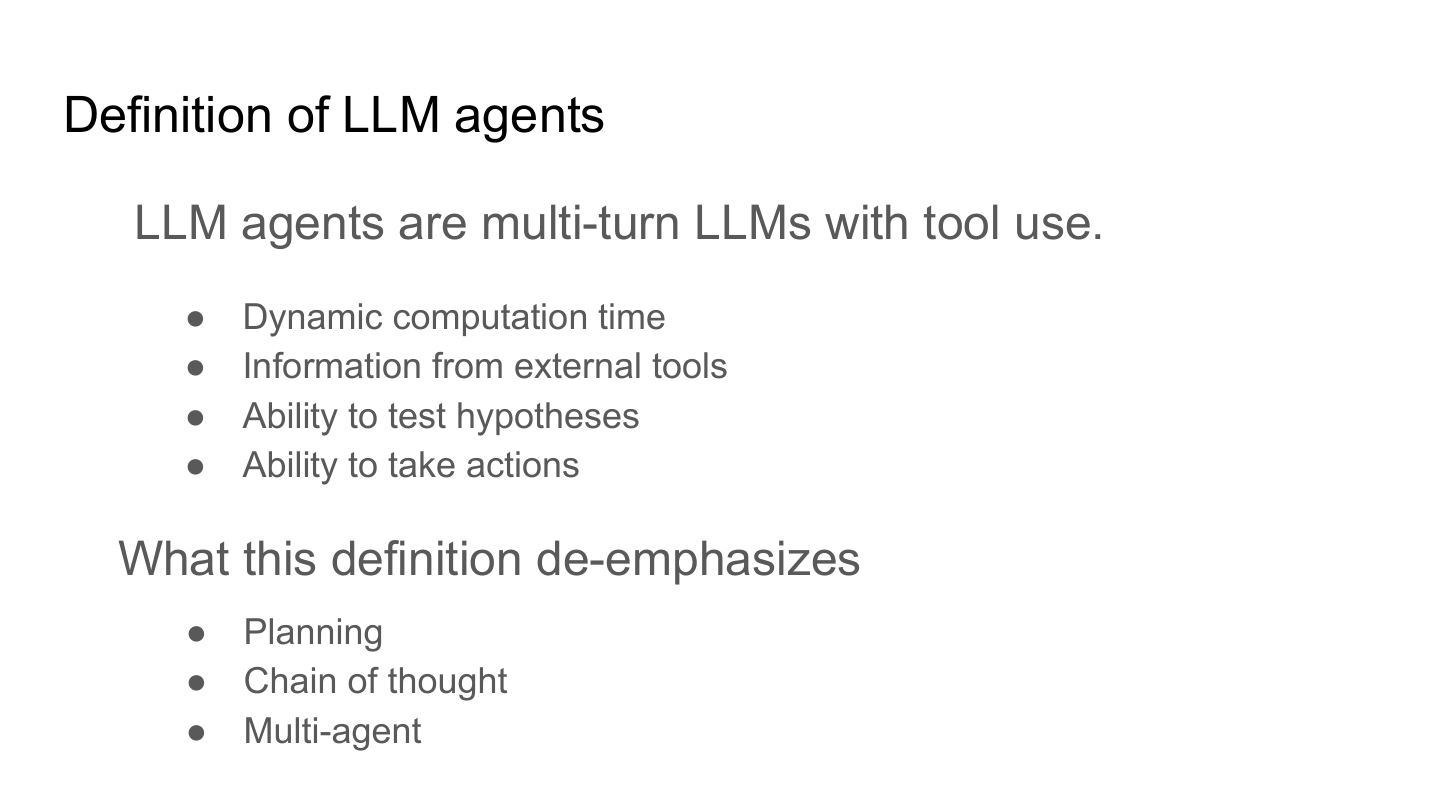
\includegraphics[width=0.78\textwidth]{../lectures/lec05_coding_agents_vulnerability_detection/figures/lec05_fig_001.png}
\caption{Sutton 的 LLM agent 定义：多轮、带工具、可测试假设、可采取行动。}
\end{figure}

\begin{figure}[H]
\centering
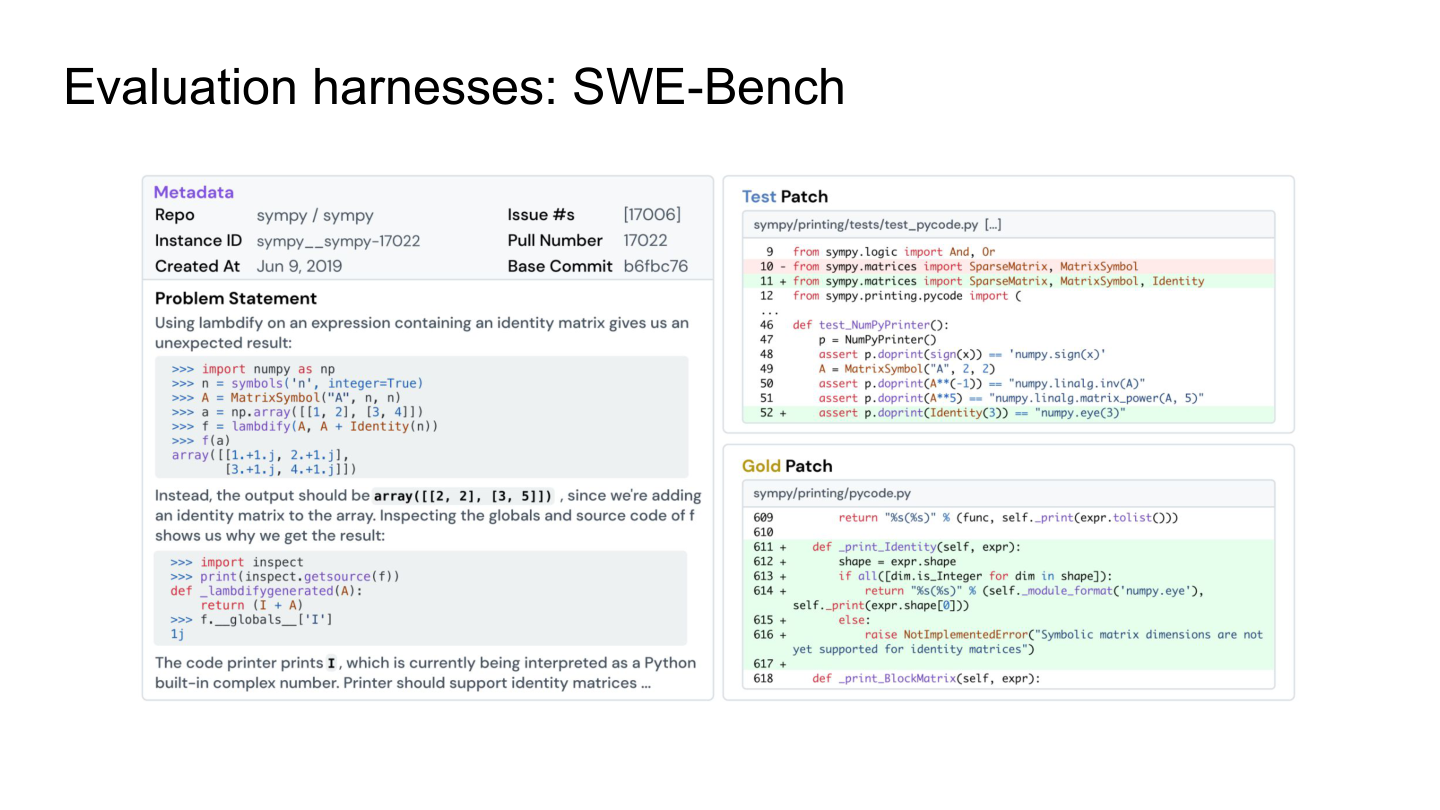
\includegraphics[width=0.8\textwidth]{../lectures/lec05_coding_agents_vulnerability_detection/figures/lec05_fig_002.png}
\caption{SWE-Bench 这类 evaluator 改变了 coding agent 设计方向：系统不再只做单函数合成，而是要处理真实仓库中的定位、修改和验证。}
\end{figure}

\[
\\operatorname{pass@k} = 1 - \\frac{{n-c \\choose k}}{{n \\choose k}}
\]

这个公式对应 lecture 中对 pass@k 的统计解释。$n$ 是总样本数，$c$ 是其中正确样本数，$k$ 表示允许查看或执行的样本数。它的工程意义在于：它既衡量正确率，也间接衡量样本多样性。但 Sutton 同时提醒，pass@k 是否合理，还取决于它是否贴近真实产品使用方式。

\begin{knowledgebox}{本讲的第一原则}
如果 evaluator 不能代表真实工作流，agent architecture 很容易被优化到错误方向。也就是说，benchmark 不是测量工具而已，它会塑造你最终造出来的系统。
\end{knowledgebox}

\section{coding agent 的核心：控制流与工具接口}
\subsection{ReAct 与动态 tool-using agent}
Lecture 中的 SWE-Agent 是动态 coding agent 的代表。其基本思想很简单：LLM 根据当前 trajectory 提出下一步动作，系统运行工具，再把输出追加回 trajectory，直到成功、超时或失败。

\begin{figure}[H]
\centering
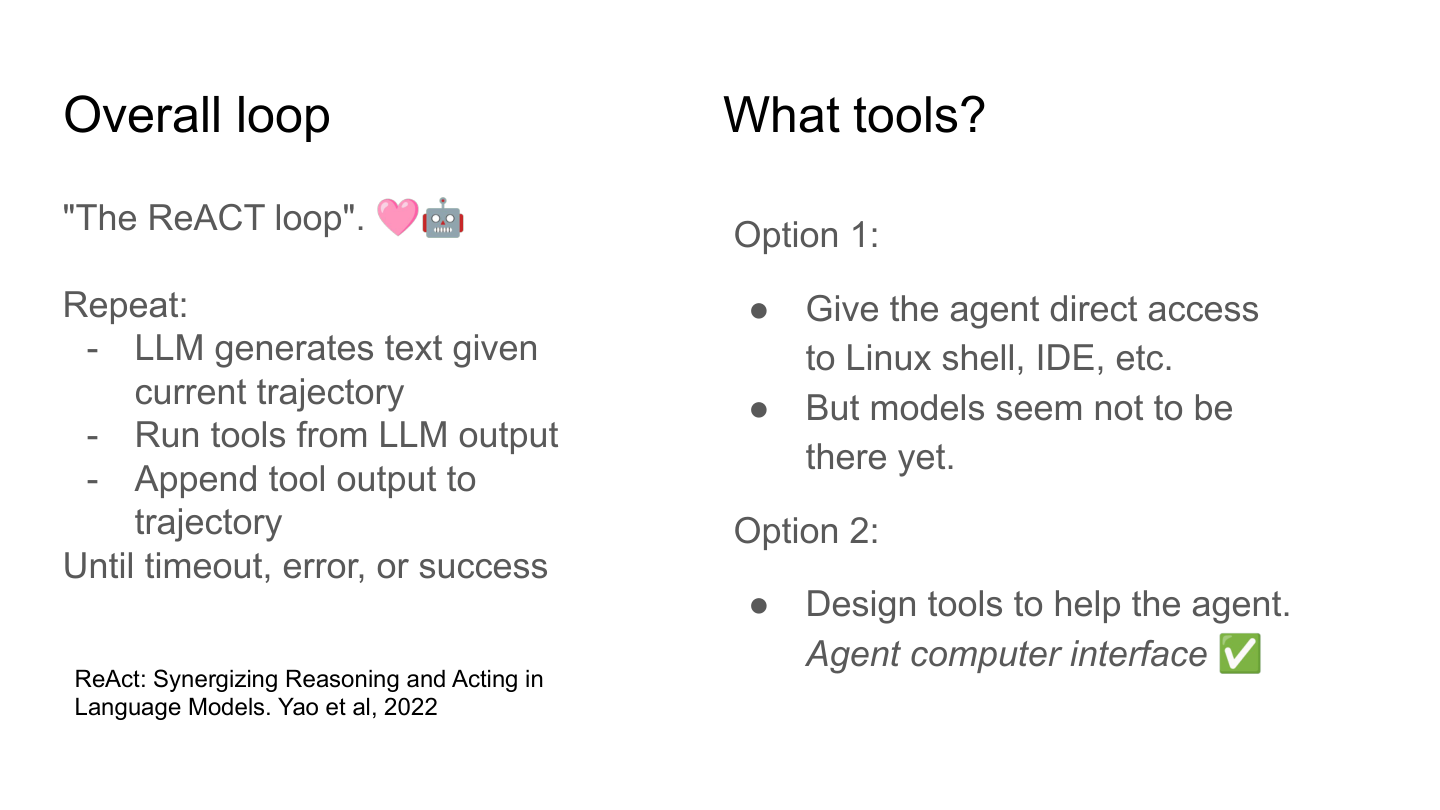
\includegraphics[width=0.76\textwidth]{../lectures/lec05_coding_agents_vulnerability_detection/figures/lec05_fig_003.png}
\caption{ReAct loop：thought/action/observation 的循环是 coding agent 最经典的最小控制结构。}
\end{figure}

\[
\\tau = (o_1, a_1, o_2, a_2, \\ldots), \\qquad \\max_{\\pi} \\mathbb{E}[R(\\tau)] \\ \\text{s.t.} \\ |\\tau| \\le B
\]

这个抽象表达了 lecture 对 agent trajectory 的理解：你优化的是整条轨迹 $\\tau$ 的成功率，而不是单次文本输出；同时轨迹长度受预算 $B$ 约束。这比“让模型多想一点”更具体，因为每一步都有工具成本、噪声和延迟。

\begin{lstlisting}
trajectory = []
while not done and budget_left():
    action = llm(trajectory)
    observation = run_tool(action)
    trajectory.append((action, observation))
\end{lstlisting}

Sutton 对 agent-computer interface 的要求很值得教材化记录：工具要简单、反馈要紧凑、动作空间要鼓励高信息密度而不是长篇废话、并且必须有 guardrails。这说明 agent intelligence 的相当一部分，其实来自 interface design。

\begin{figure}[H]
\centering
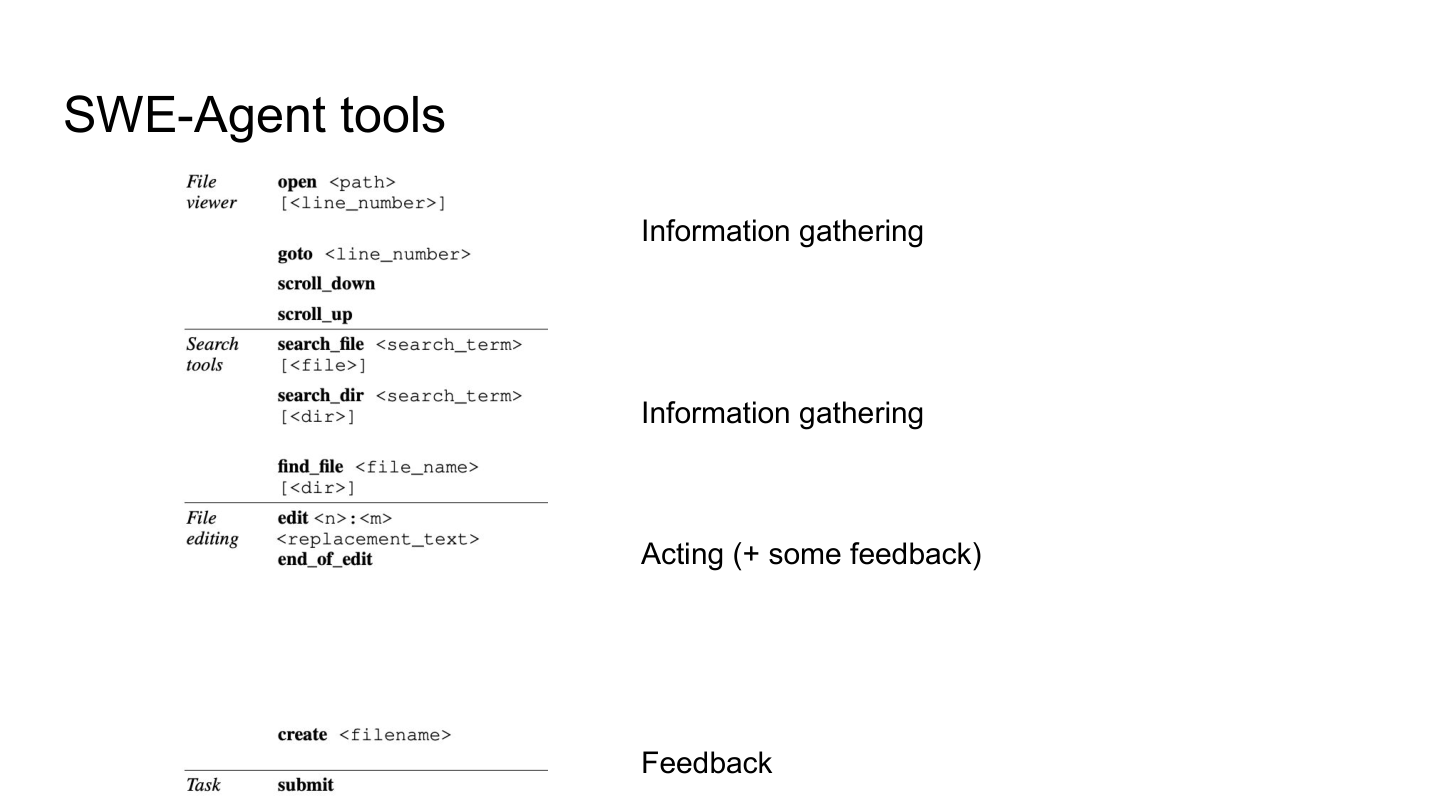
\includegraphics[width=0.82\textwidth]{../lectures/lec05_coding_agents_vulnerability_detection/figures/lec05_fig_004.png}
\caption{SWE-Agent 的工具层次：信息收集、行动和反馈构成闭环。}
\end{figure}

\subsection{Agentless、AutoCodeRover 与 procedural control}
Sutton 讲得非常清楚：并不是所有 coding task 都需要最高自由度的动态 agent。Agentless 和 AutoCodeRover 展示了一类 procedural control：先把大工作流写出来，例如 localization、patch generation、ranking，然后在局部节点调用模型。它们的价值是更稳定、更容易调试，也更容易把 test-time compute 投到确定的阶段上。

\begin{figure}[H]
\centering
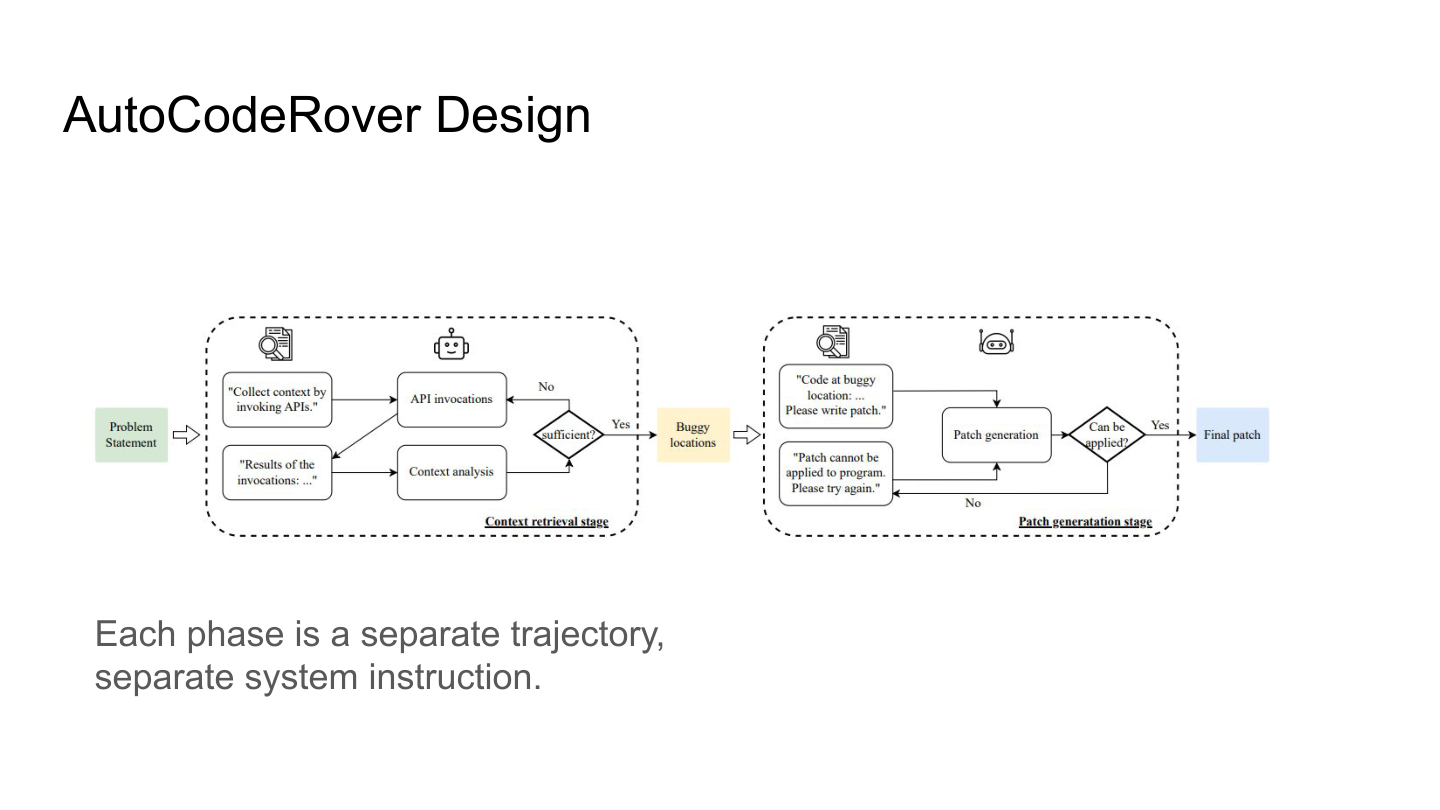
\includegraphics[width=0.76\textwidth]{../lectures/lec05_coding_agents_vulnerability_detection/figures/lec05_fig_005.png}
\caption{AutoCodeRover 的阶段式设计：每一阶段有独立 trajectory 和独立 instruction，是介于静态 pipeline 与完全动态 agent 之间的折中。}
\end{figure}

\begin{lstlisting}
files = localize_issue(repo, bug_report)
patches = synthesize_candidate_patches(files)
ranked = rerank_with_tests(patches)
return ranked[0]
\end{lstlisting}

这类设计解决的问题是可控性。若 workflow 本身相对固定，把控制流外移到显式 Python/状态机中，往往比把一切交给 LLM 更可靠。代价是探索能力受限，遇到奇怪错误时可能不如动态 agent 灵活。

\subsection{design space：真正要调的是哪几个旋钮}
Passerine 和 design-space slides 提供了一个很好的统一框架：你实际上在同时设计 tools、control flow、prompting/memory。它们彼此耦合。例如工具很多且噪声大时，过度动态的 agent 会反复迷路；任务很开放时，纯 procedural pipeline 又会过早锁死策略空间。

\begin{lstlisting}
design = {
  'tools': ['search', 'edit', 'execute', 'feedback'],
  'control_flow': ['procedural', 'state_machine', 'dynamic', 'tree_search'],
  'prompting': ['system role', 'phase instructions', 'memory']
}
\end{lstlisting}

\begin{importantbox}{dynamic 和 procedural 不是价值观之争}
Lecture 的真正问题是：test-time compute 应该放在哪。是让 agent 在单条轨迹里自由探索，还是把预算分配给更窄但更稳定的程序化阶段？这和第一讲、第四讲关于 test-time compute 的讨论直接相连。
\end{importantbox}

\section{从 coding tasks 到 security tasks}
安全任务与普通 coding tasks 的关键区别，不在于“代码更难”，而在于 evaluator 更硬、环境更复杂、验证更重要。CTF 任务要求 agent 理解协议、交互式程序、二进制、网络服务和 exploit 条件，很多时候单看源码根本不够。

\begin{figure}[H]
\centering
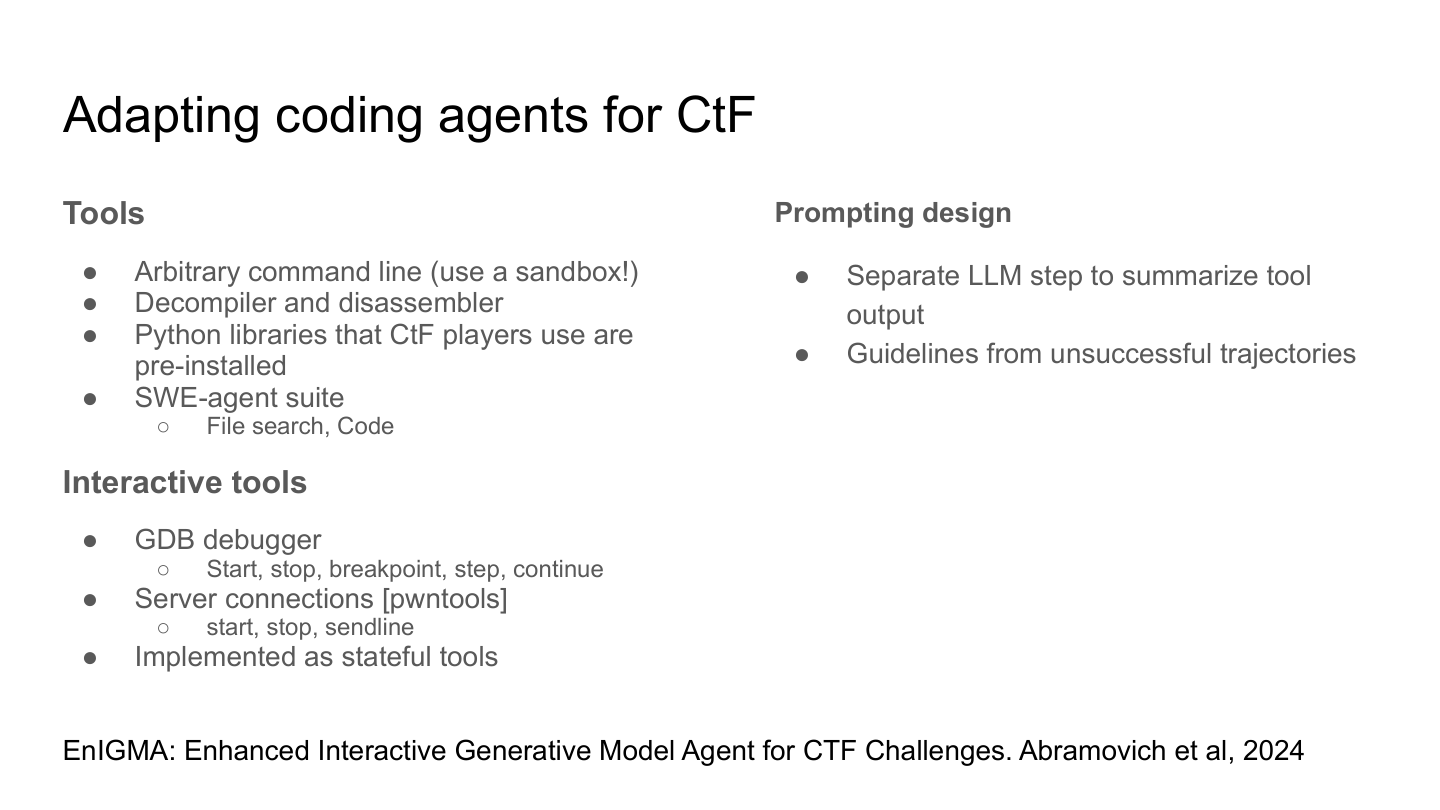
\includegraphics[width=0.8\textwidth]{../lectures/lec05_coding_agents_vulnerability_detection/figures/lec05_fig_006.png}
\caption{EnIGMA 的 interactive tools：debugger、server connection、shell 与 Python 工具让 agent 能进入安全问题真正的状态空间。}
\end{figure}

\begin{lstlisting}
while not solved:
    tool_call = lm.choose(['shell', 'debugger', 'server', 'python'])
    obs = execute(tool_call)
    update_context(obs)
    if flag_found(obs):
        break
\end{lstlisting}

《EnIGMA》reading 把 lecture 的直觉变成了证据：交互式工具显著提升了 security agents 在 CTF benchmark 上的表现。这说明安全 agent 不是普通 coding agent 加一句 “think like a hacker” 就能得到的；它需要完全不同的信息接口和验证接口。

但教材化地看，EnIGMA 的价值和边界都要同时看到。它证明 interactive tools 能显著改变 security-task performance，这一点非常重要；可它主要仍然是在 CTF-style environment 中验证方法。CTF 的好处是目标清晰、反馈直接、flag 导向明确，因此它非常适合回答“如果给 agent debugger、server connection 与 shell，会不会更强”。可它不自动回答另一个更难的问题：\textbf{这些能力能否稳定迁移到真实生产仓库中的长期漏洞研究？}

这正是 lecture 后半段转向 Big Sleep 的原因。Sutton 并不是否定 CTF benchmark，而是把它放在一个更大的 capability ladder 里：CTF 先证明工具接口有价值；真实仓库研究再检验 agent 能否在更稀疏、更含糊、更多上下文依赖的环境里发挥作用。

\section{漏洞检测：为什么“看起来像 bug”远远不够}
Slides 在漏洞检测部分很务实。一个 software vulnerability 不只是程序错误，而是具有安全含义的程序错误，例如 XSS、越界读写、SQL 注入、use-after-free 等。判断这类问题通常需要：
\begin{itemize}
\item 更大的全局上下文，而不是单个函数的局部文本。
\item 对输入约束、调用路径与 exploitability 的理解。
\item 来自执行、sanitizer、fuzzing 或其他分析器的验证信号。
\item 结合历史补丁和 CVE 语境做 variant analysis。
\end{itemize}

因此，普通编程 benchmark 上的高分并不自动转化为高质量 vulnerability detection。Sutton 专门把 NVD、AI Cyber Challenge、传统 fuzzing/static analysis 放进同一段，就是为了强调：安全 agent 应该与这些已有验证工具协作，而不是取代它们。

\section{Big Sleep：真实仓库中的 variant analysis agent}
Lecture 最关键的 case study 是 Big Sleep。它之所以重要，不仅因为它找到了真实世界漏洞，更因为它选择了一个更可信的任务 framing：variant analysis。也就是说，不让 agent 在无限开放的仓库空间里瞎逛，而是利用 recent commits、diffs、历史 bug patterns 作为 seed hint，围绕这些线索做针对性搜索。

\begin{figure}[H]
\centering
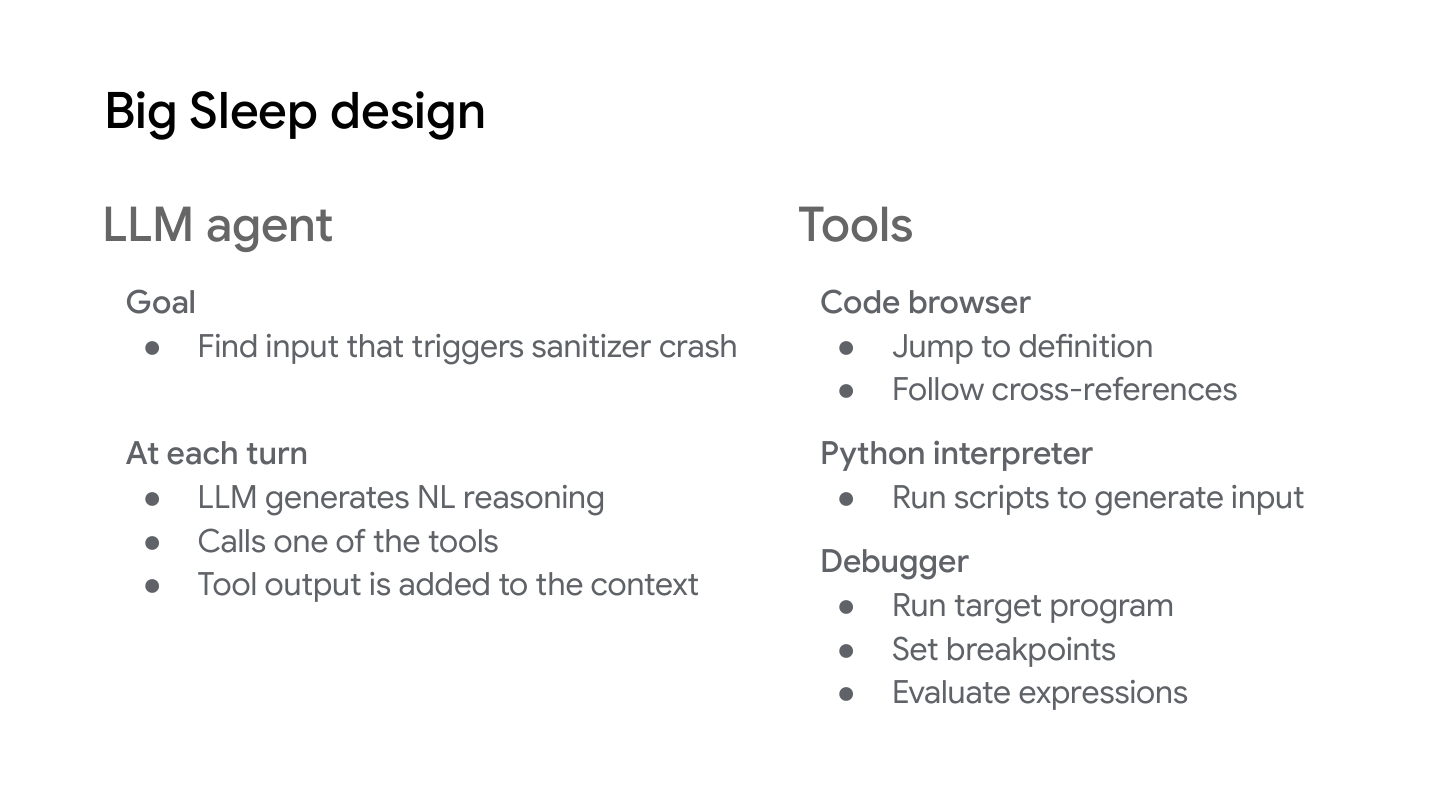
\includegraphics[width=0.8\textwidth]{../lectures/lec05_coding_agents_vulnerability_detection/figures/lec05_fig_007.png}
\caption{Big Sleep 的工作流：从代码浏览、到工具执行、到 hypothesis revision，核心是 tool-grounded variant analysis。}
\end{figure}

\[
\\max_{a_{1:T}} \\ \\Pr\\big[V(\\text{{repo}}, a_{1:T}) = 1 \\mid \\text{{seed hint}}\\big]
\]

这个抽象表达了 variant-analysis workflow 的本质：不是最大化“模型能否想出漏洞故事”，而是最大化在 seed hint 条件下，通过动作序列 $a_{1:T}$ 找到可被 verifier 证实的真实问题的概率。这里的 verifier 可以是 sanitizer crash、真实 exploit signal 或其它独立证据。

\begin{lstlisting}
for diff in recent_security_relevant_commits:
    hypothesis = llm.propose_variant(diff)
    trace = browse_repo_and_execute(hypothesis)
    if verifier(trace):
        report_vulnerability(trace)
\end{lstlisting}

Project Zero 的 Big Sleep 文章进一步说明了 lecture 没有完全展开的两点。第一，真实成果依赖 repository context 和 diff-aware prompting，而不是纯文本问答。第二，这项工作被明确放在防御者视角：在漏洞正式发布前发现并修补它，减少攻击者可利用窗口。

把《EnIGMA》和 Big Sleep 放在一起看，本讲其实给出了一条很清楚的 security-agent 递进路线：
\begin{itemize}
\item 先在 CTF 或 sandboxed challenge 中验证 \textbf{tool interface} 是否真的改善搜索与验证。
\item 再在真实仓库里使用 diff、recent commits、历史补丁模式等线索，把任务重构成更可控的 \textbf{variant analysis}。
\item 最后才讨论更开放的 defensive deployment，包括 provenance、sandbox、日志、权限控制和 human escalation。
\end{itemize}

这样看，Big Sleep 不是“模型忽然更聪明了”的故事，而是 lecture 全程都在强调的同一个原则：\textbf{高风险 agent 的价值来自 workflow grounding，而不是语言流畅性。}

\begin{figure}[H]
\centering
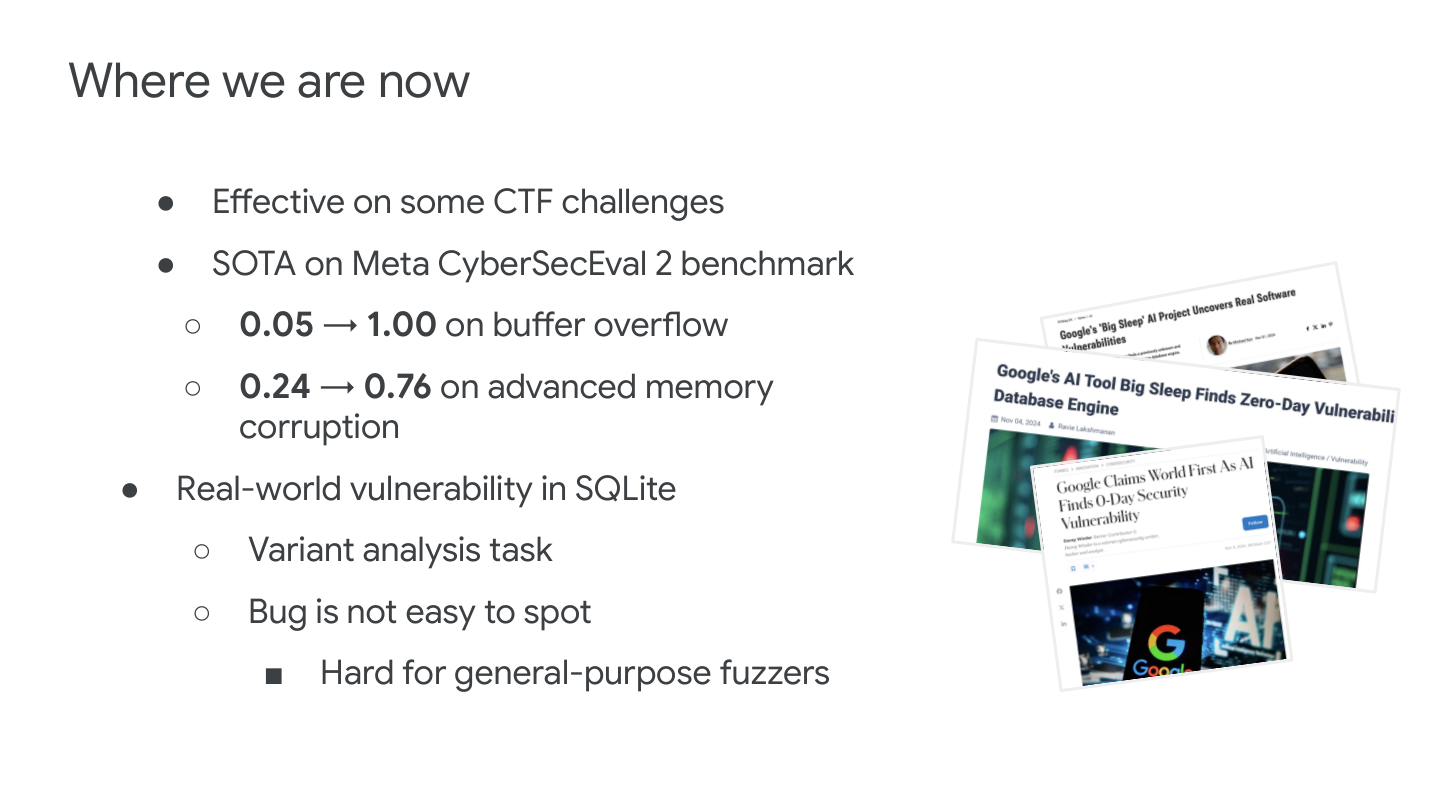
\includegraphics[width=0.82\textwidth]{../lectures/lec05_coding_agents_vulnerability_detection/figures/lec05_fig_008.png}
\caption{结果页体现的不是“模型更聪明”而是“workflow 更 grounded”：工具、验证和环境反馈让安全 agent 真正具备可交付价值。}
\end{figure}

\begin{warningbox}{安全 agent 的关键风险}
如果缺少 sandbox、工具权限约束、日志与 provenance 记录，security agent 可能同时变得不安全、不可审计，也无法复现实验结果。高风险任务中的 agent 设计，必须把 guardrails 当作一等公民。
\end{warningbox}

\section{与前后讲的关系、本章小结与复习}
本讲与 L04 的关系很直接：上一讲讨论 verifier 和 recipe，L05 则把这些思想带到 coding agents 和 vulnerability detection 中。系统不是靠“会说更复杂的 chain-of-thought”取胜，而是靠 evaluator、tool interface 和 environment feedback 形成闭环。

\section{本章小结}
本讲最重要的结论是：coding agents 的核心不是某个华丽 prompt，而是 control flow、工具接口和 evaluator 的共同设计。越到 security 这种高风险领域，越不能把“模型说得像”当成“系统真的对”；必须通过工具、执行和 verifier 建立 grounded workflow。

\section{复习题}
\begin{itemize}
\item 为什么 Sutton 把 evaluator 放在 coding-agent 设计的起点？
\item ReAct, Agentless, AutoCodeRover 在控制流上分别有什么差异？
\item 为什么 CTF/security tasks 更依赖 interactive tools？
\item 什么是 variant analysis，为什么它比开放式漏洞搜索更现实？
\item 为什么 security agent 必须把 sandbox 和 provenance 放进系统设计？
\end{itemize}

\section{深入思考题}
\begin{itemize}
\item 在什么 benchmark 条件下，dynamic agent 的优势会被 procedural pipeline 吃掉？
\item 安全 agent 的 verifier 应该如何设计，才能既减少误报又避免 reward hacking？
\item 如果给 Big Sleep 更多 test-time compute，应该优先加在 tool diversity、trajectory depth 还是 hypothesis generation 上？为什么？
\end{itemize}

\section{延伸阅读}
\begin{itemize}
\item EnIGMA: Interactive Tools Substantially Assist LM Agents in Finding Security Vulnerabilities
\item From Naptime to Big Sleep: Using Large Language Models To Catch Vulnerabilities In Real-World Code
\end{itemize}

\part{Multimodal and Interactive Agents}
\chapter{Multimodal Autonomous AI Agents}
\label{chap:lec06_multimodal_autonomous_agents}
\section{本讲学习目标}

本讲把“多模态 agent”从一个流行术语拆成可以操作的系统问题。读完后，读者应能回答：
\begin{itemize}
\item 为什么真实的 multimodal autonomous agents 首先出现在网页、桌面和机器人等交互环境，而不是单张图片问答。
\item 为什么 \textbf{Mind2Web}、\textbf{WebArena}、\textbf{VisualWebArena} 分别对应不同的 benchmark 假设，不能混为一谈。
\item 为什么网页 agent 的核心难题不是“能不能 OCR”，而是 \textbf{视觉 grounding、长程规划、环境反馈、执行正确性} 的耦合。
\item 为什么 \textbf{Tree Search for Language Model Agents} 是 inference-time computation 在 web agents 上的典型用法。
\item 为什么 agent 训练会遇到严重的数据瓶颈，以及 \textbf{InSTA} 一类 synthetic task pipeline 想解决什么问题。
\item 为什么讲者在最后把话题从 web tasks 推向 physical agents，并用 \textbf{Plan-Seq-Learn} 说明感知、规划和低层控制的分层关系。
\end{itemize}

\section{背景与问题设置}

\subsection{Autonomous agents 的任务不是静态问答，而是长程交互}

讲者一开头就把多模态 autonomous agents 放回到现实工作流里：很多高价值任务本来就在电脑上完成，而且经常发生在网页上。于是 agent 的问题就从“给一张图回答一个问题”变成了“在真实界面上执行一串可验证的动作”。这一点决定了本讲的主语不是视觉模型本身，而是 \textbf{带有 environment feedback 的 multimodal agent}。

\begin{figure}[H]
\centering
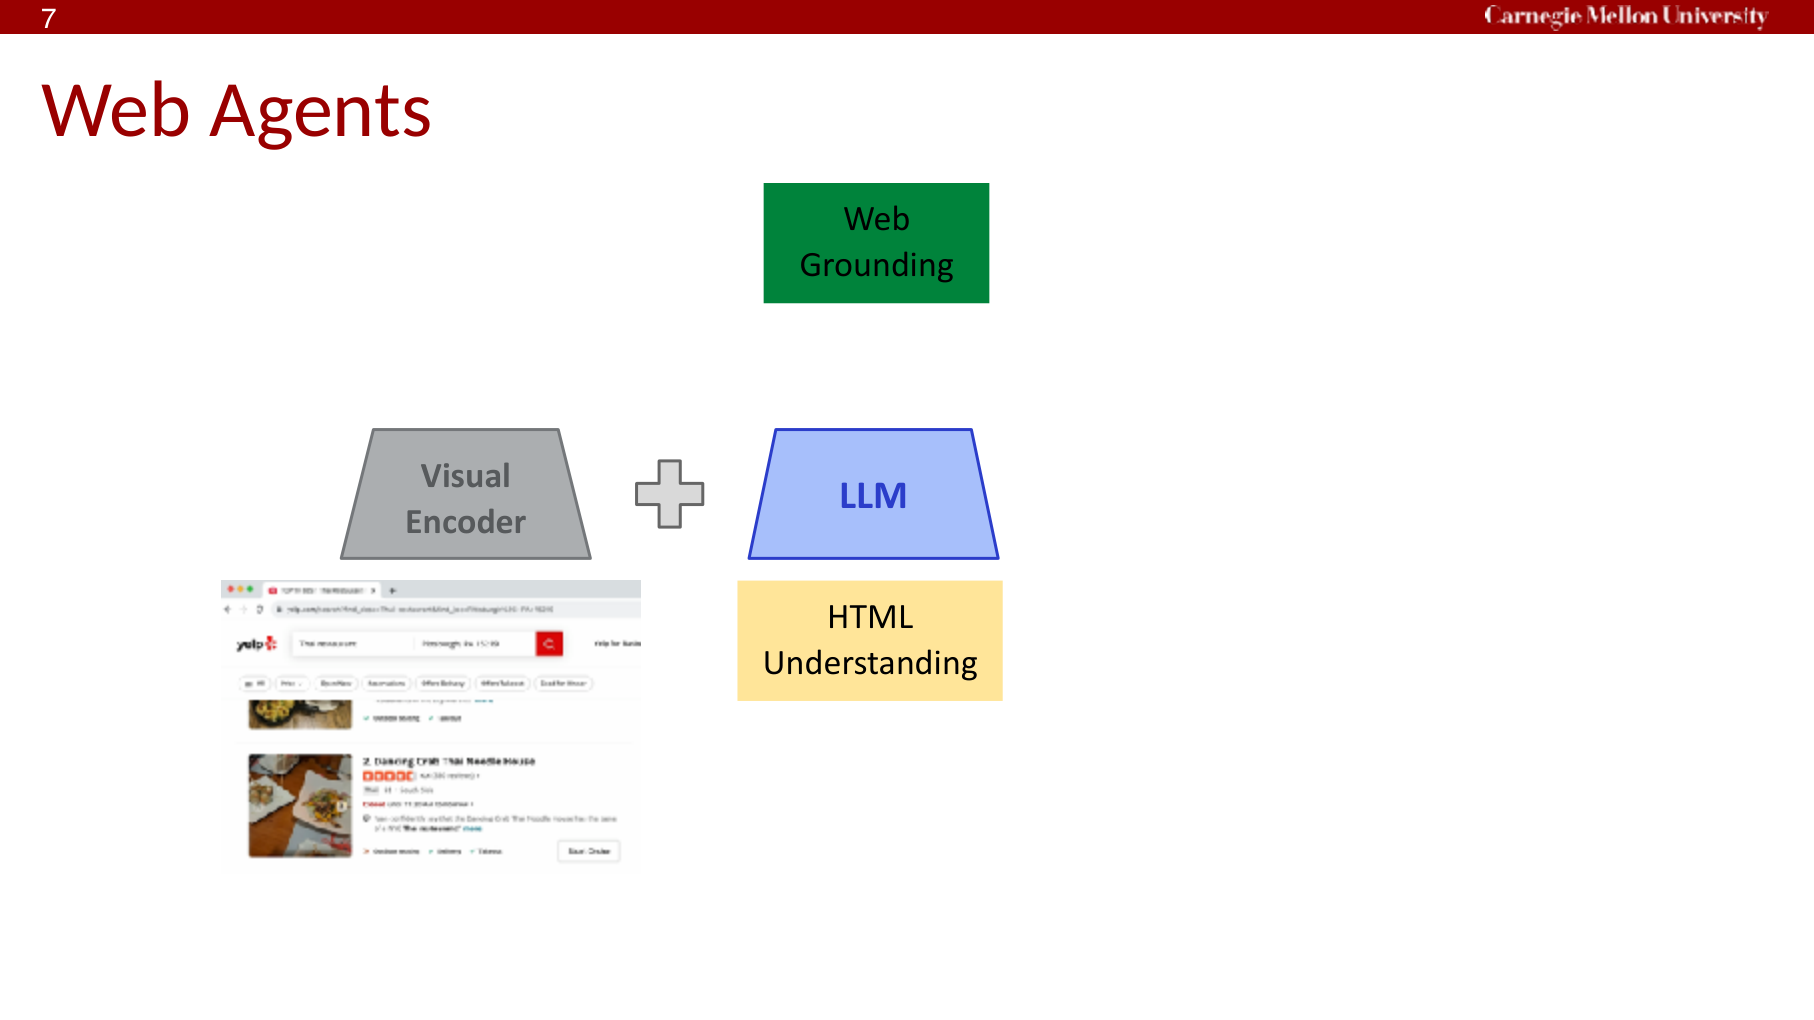
\includegraphics[width=0.82\textwidth]{../lectures/lec06_multimodal_autonomous_agents/figures/lec06_fig_001.png}
\caption{Web agents 的基本栈：视觉、语言、grounding 与网页环境共同决定 agent 的行为。}
\end{figure}

如果任务是“找一个评分最高、评论数超过 200 的泰餐厅”，系统不能只做信息检索。它还要在页面之间跳转、读取视觉元素、区分可点击区域、判断排序结果、避免误操作，并在达到目标后停止。这类问题天然具有三个结构特征：
\begin{itemize}
\item \textbf{部分可观测（partial observability）}：agent 看到的只是当前屏幕和局部 DOM，而不是真实网页状态的完整描述。
\item \textbf{长程交互（long horizon interaction）}：要多步连续做对，不能把任务拆成彼此独立的单跳问答。
\item \textbf{执行正确性（functional correctness）}：很多任务的答案不是一段文本，而是页面状态是否被正确改变、仓库是否被创建、购物流程是否真的完成。
\end{itemize}

这就是为什么本讲会把 \textbf{benchmark realism} 放在第一优先级。没有真实环境，很多 agent 错误根本暴露不出来。

\subsection{为什么纯 HTML 不够：视觉 grounding 是任务语义的一部分}

WebArena 之前的很多方法倾向于把网页转成 HTML、accessibility tree 或压缩后的文本表示，再让 LLM 在文本空间里做决策。这当然有价值，但讲者明确指出 \textbf{HTML is insufficient}。原因不是 HTML 完全没信息，而是现实网页中有大量决定任务成败的内容并不稳定地出现在文本表示里：
\begin{itemize}
\item CSS/JavaScript 动态改变布局与可见状态。
\item 可点击元素的真实位置、层叠关系与视觉显著性不等价于 DOM 顺序。
\item 视觉上下文经常决定“这个按钮是不是用户想要的那个按钮”。
\item 真实任务包含图片比对、商品外观匹配、截图中的表格或地图等视觉约束。
\end{itemize}

这意味着 \textbf{视觉信息并不是附加模态，而是任务语义本身}。当用户说“买这个图里同款但红色的另一个商品”时，文本树再长也不足以替代视觉 grounding。

\begin{knowledgebox}{本讲的核心命题}
对真实 web agents 来说，感知和规划不是两个彼此独立的问题。观测表示一旦失真，后续规划再强也只是在错误状态上做聪明搜索。
\end{knowledgebox}

\section{Benchmark 视角：Mind2Web、WebArena 与 VisualWebArena}

\subsection{三者分别回答什么问题}

这三套资源经常被放在同一条 agent 发展线上，但它们回答的问题并不一样。

\textbf{Mind2Web} 的重点是 \emph{generalist web-agent data}。它收集 137 个真实网站、31 个 domain 上的 2000 多个开放式任务与人工动作序列，目的是让研究者能在真实网站分布上研究泛化。它告诉我们：真实网站远比模拟环境复杂，HTML 也远比玩具环境中的结构化描述更脏、更长、更噪。

\textbf{WebArena} 的重点是 \emph{realistic yet reproducible environment}。它不只给演示数据，而是给出可交互环境、工具站点、知识资源和 execution-based functional checks。也就是说，WebArena 更接近“真实任务环境”，而不是静态轨迹数据集。

\textbf{VisualWebArena} 则继续追问：如果现实网页任务需要图片、布局、界面视觉提示，那么 text-only environment 仍然低估了问题难度。它在 WebArena 的基础上加入 visually grounded tasks 和 visually grounded evaluation，使 benchmark 真正开始衡量多模态网页 agent。

\begin{importantbox}{关键区分}
Mind2Web 偏向 \textbf{离线真实网页数据集}；WebArena 偏向 \textbf{可交互、可复现、execution-based 的文本为主环境}；VisualWebArena 则把同样的 functional evaluation 推向 \textbf{视觉 grounding 必不可少} 的任务空间。
\end{importantbox}

\subsection{VisualWebArena：把视觉放回 functional evaluation}

\begin{figure}[H]
\centering
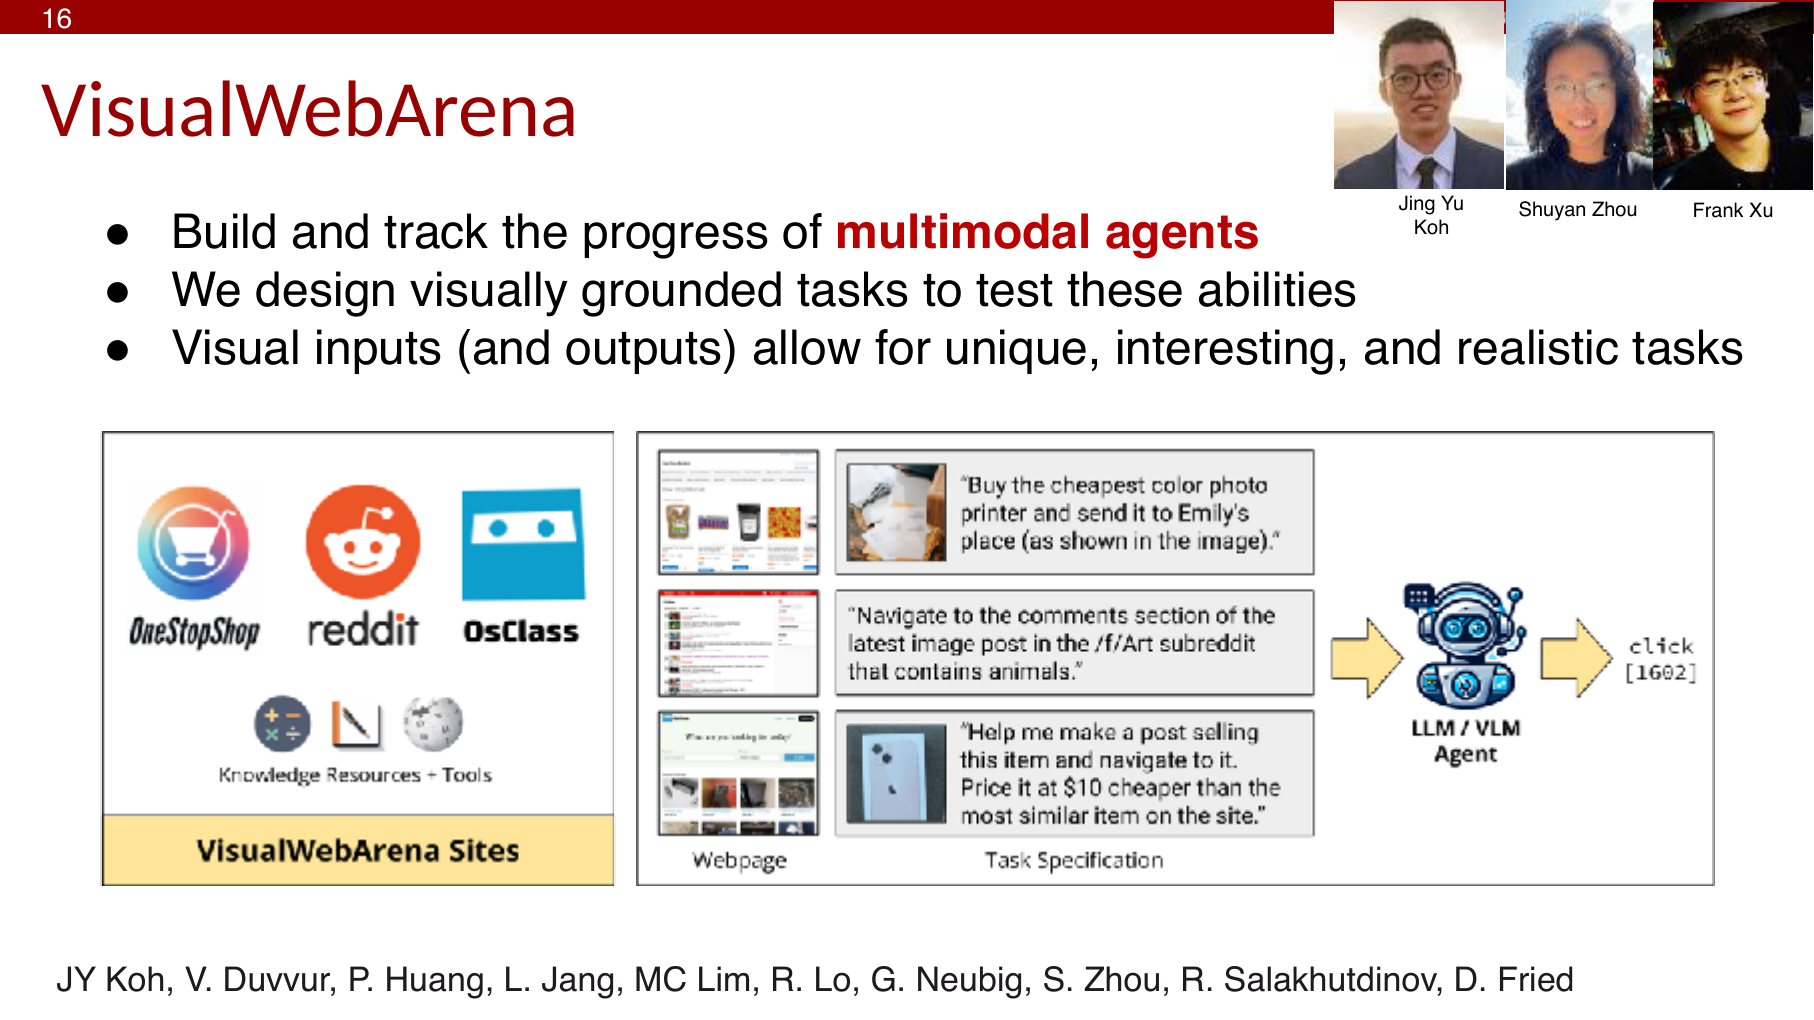
\includegraphics[width=0.82\textwidth]{../lectures/lec06_multimodal_autonomous_agents/figures/lec06_fig_002.png}
\caption{VisualWebArena 的目标是 visually grounded web tasks，而不是只在文本化网页上做导航。}
\end{figure}

讲者用多个任务示例说明 VisualWebArena 为什么必要。比如按图片找到同款商品、在分类广告里比对目标图片、在论坛中根据页面布局进入正确评论区，这些任务都不能靠“读一段 HTML 再回答”来完成。VisualWebArena 的价值在于：
\begin{itemize}
\item 它把 \textbf{视觉-文本联合观测} 变成 benchmark 的默认输入。
\item 它延续 WebArena 的 \textbf{execution-based evaluation}，避免只看文本表面相似度。
\item 它让研究者能定量比较 \textbf{text-based LLM agents} 与 \textbf{multimodal VLM agents} 的差异。
\end{itemize}

从形式上看，这类环境很自然地写成一个 POMDP：
\[
\mathcal{M}=(\mathcal{S},\mathcal{A},\mathcal{O},T,R),\qquad o_t\sim \mathcal{O}(s_t),\ a_t\in\mathcal{A}(o_t).
\]
其中，$\mathcal{S}$ 是网页环境真实状态，$\mathcal{A}$ 是可执行动作集合，$\mathcal{O}$ 决定 agent 在某个状态下能看到的截图、DOM 或 SoM 标记等观测，$T$ 是环境转移，$R$ 则是与 functional correctness 相关的奖励或成功判定。写成这个形式的意义在于：\textbf{agent 的难度不仅在动作选择，也在观测建模。}

\section{从 VLM Agents 到 Inference-Time Search}

\subsection{SoM、规划与 failure modes}

讲者随后转向 \textbf{Visual Language Models as Agents}。slides 强调的不是“换一个更大的 VLM 就好”，而是要给模型一种更适合交互界面的表示。Set-of-Marks（SoM）风格的表示就是代表例子：把可交互元素显式标记出来，帮助模型在图像空间中定位 candidate actions。

\begin{figure}[H]
\centering
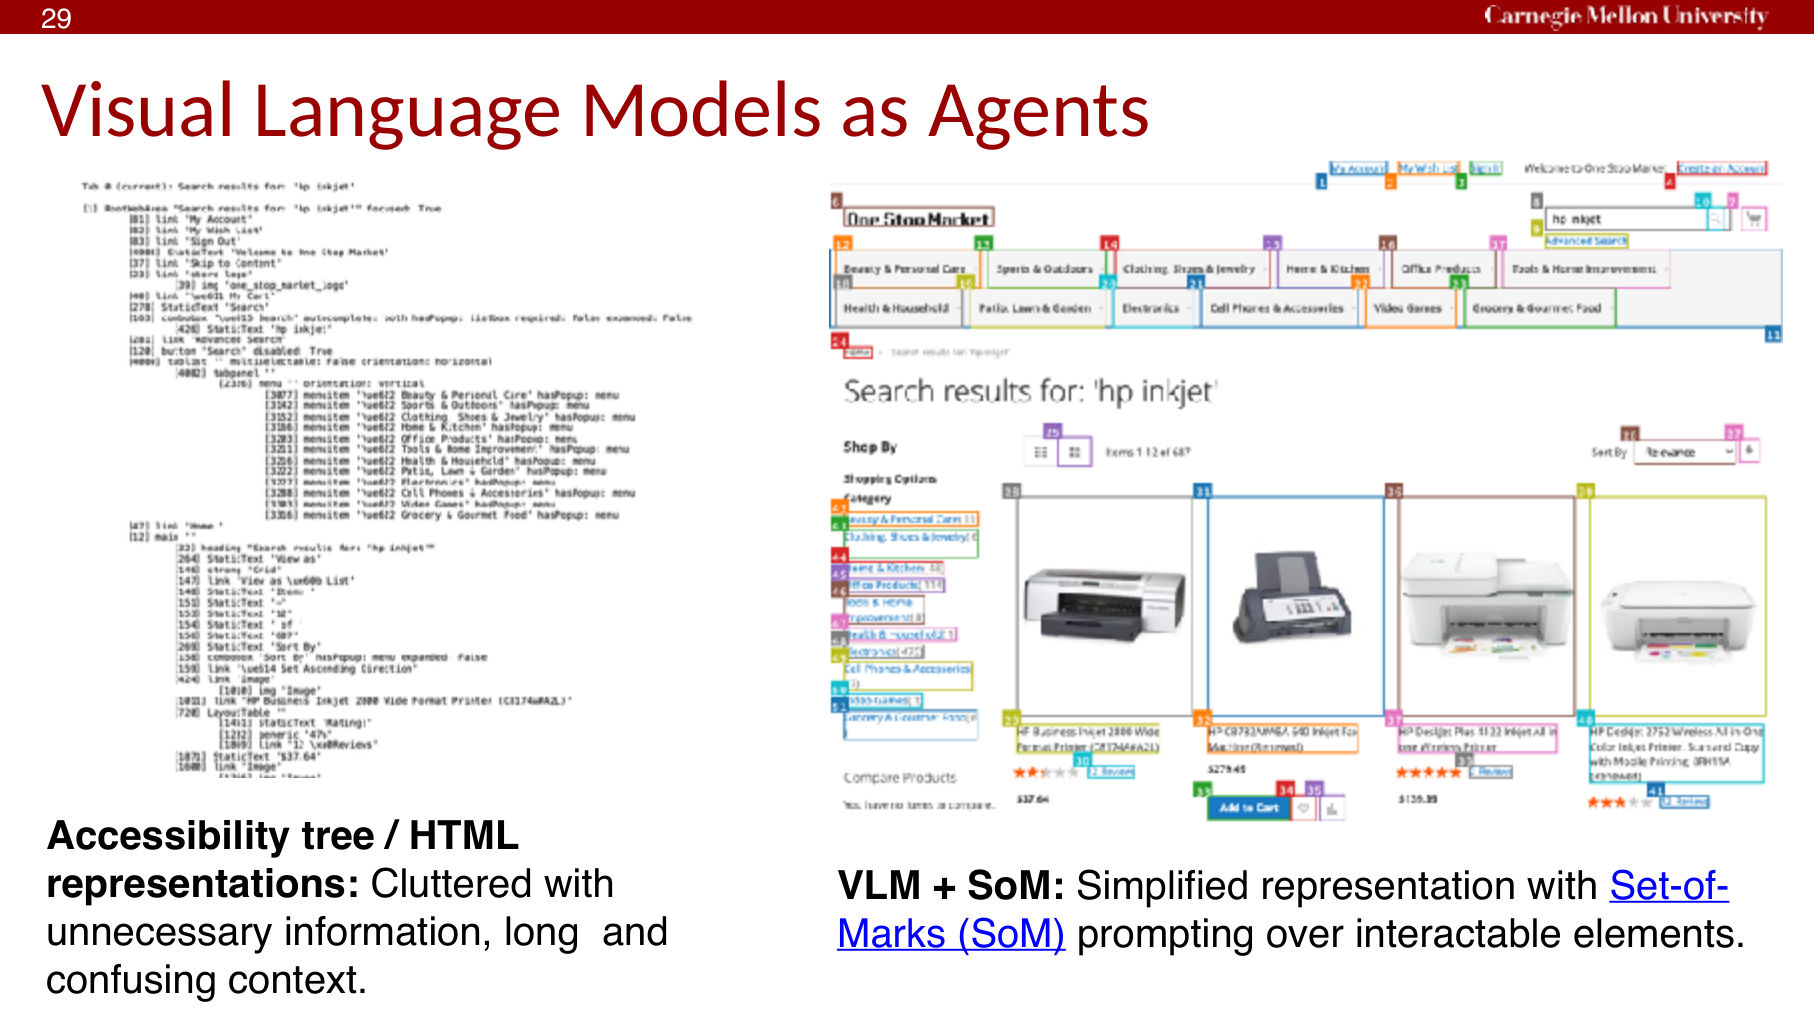
\includegraphics[width=0.72\textwidth]{../lectures/lec06_multimodal_autonomous_agents/figures/lec06_fig_003.png}
\caption{SoM 风格表示把交互元素变成更明确的视觉候选，缓解 cluttered interfaces 带来的歧义。}
\end{figure}

同时，web agent 还需要一个更完整的系统架构：
\begin{figure}[H]
\centering
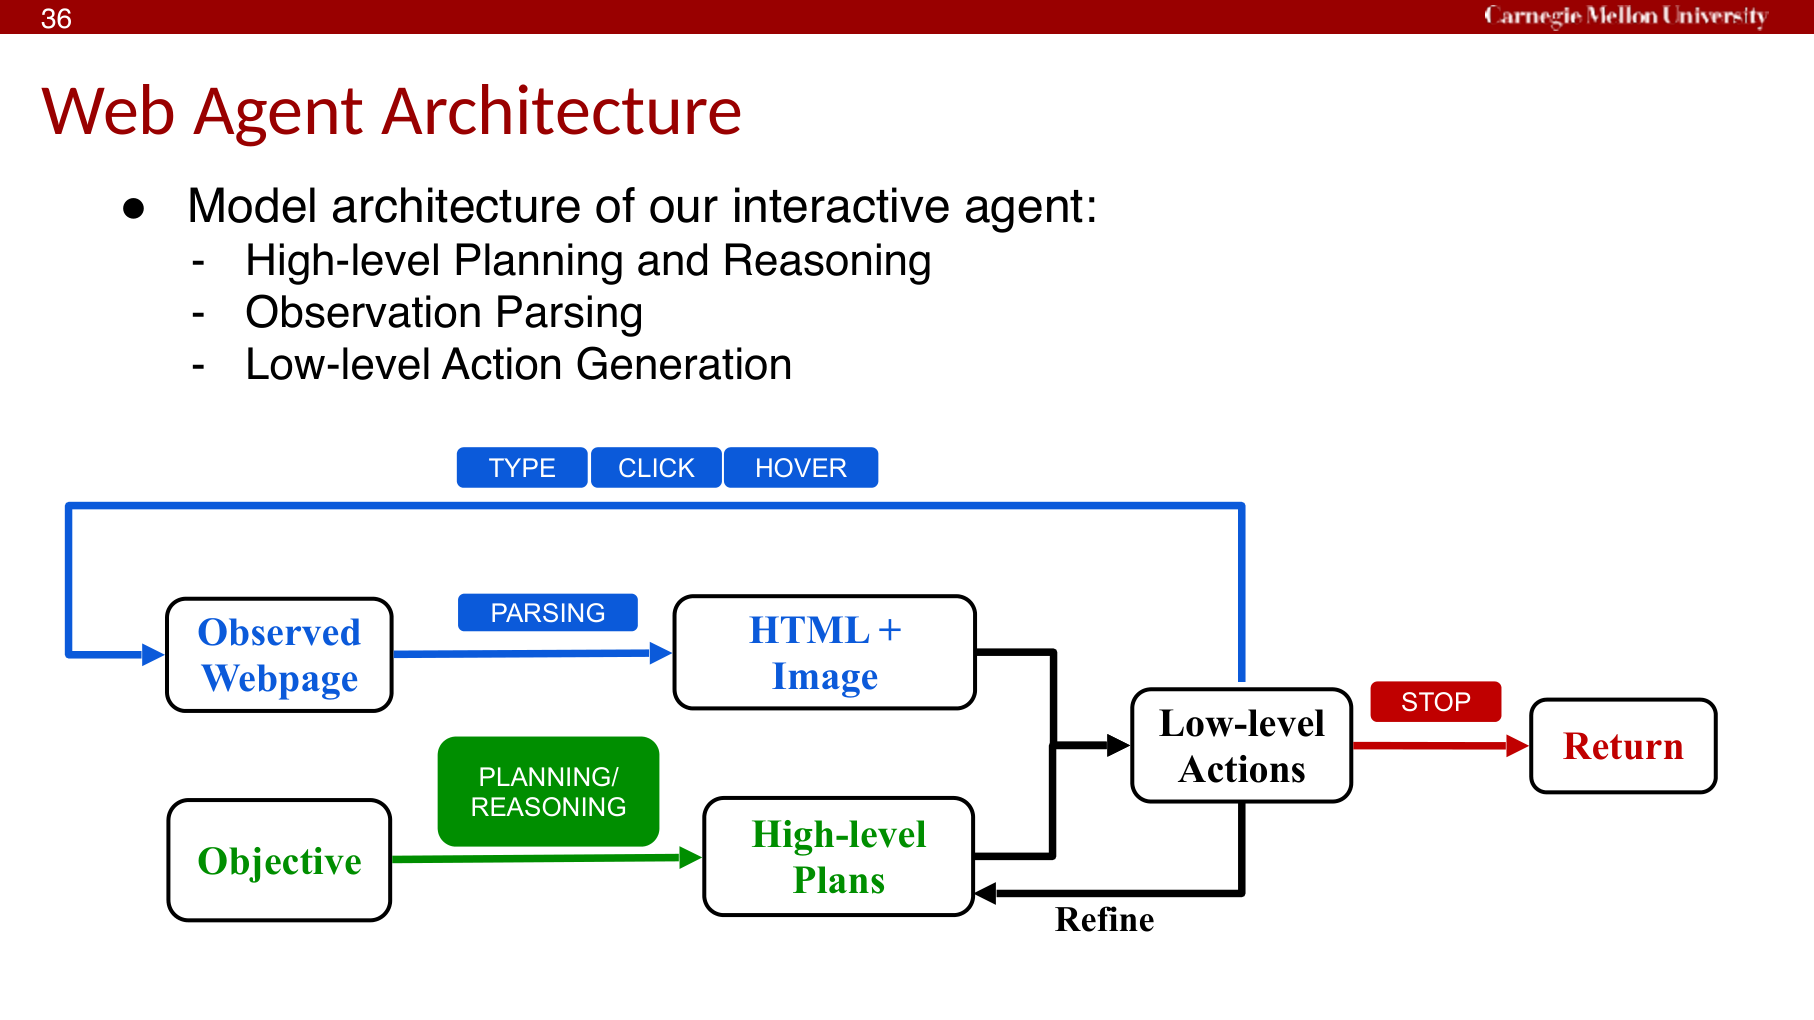
\includegraphics[width=0.80\textwidth]{../lectures/lec06_multimodal_autonomous_agents/figures/lec06_fig_004.png}
\caption{Web agent architecture 需要同时处理观测、低层动作、计划状态与环境反馈。}
\end{figure}

这里有一个关键认识：\textbf{低层动作正确，并不代表全局任务正确。} 例如某一步点击看起来合理，但会把 agent 带进错误页面；又例如 agent 一度完成了正确操作，随后又因为没有保持全局目标状态而把它撤销。这些 failure modes 在 slides 中被明确列出，包括在页面间来回 oscillate、卡在 loop 里、或者做对一部分又在后续步骤 undo 掉。

\subsection{为什么长程任务会出现 error compounding}

\begin{figure}[H]
\centering
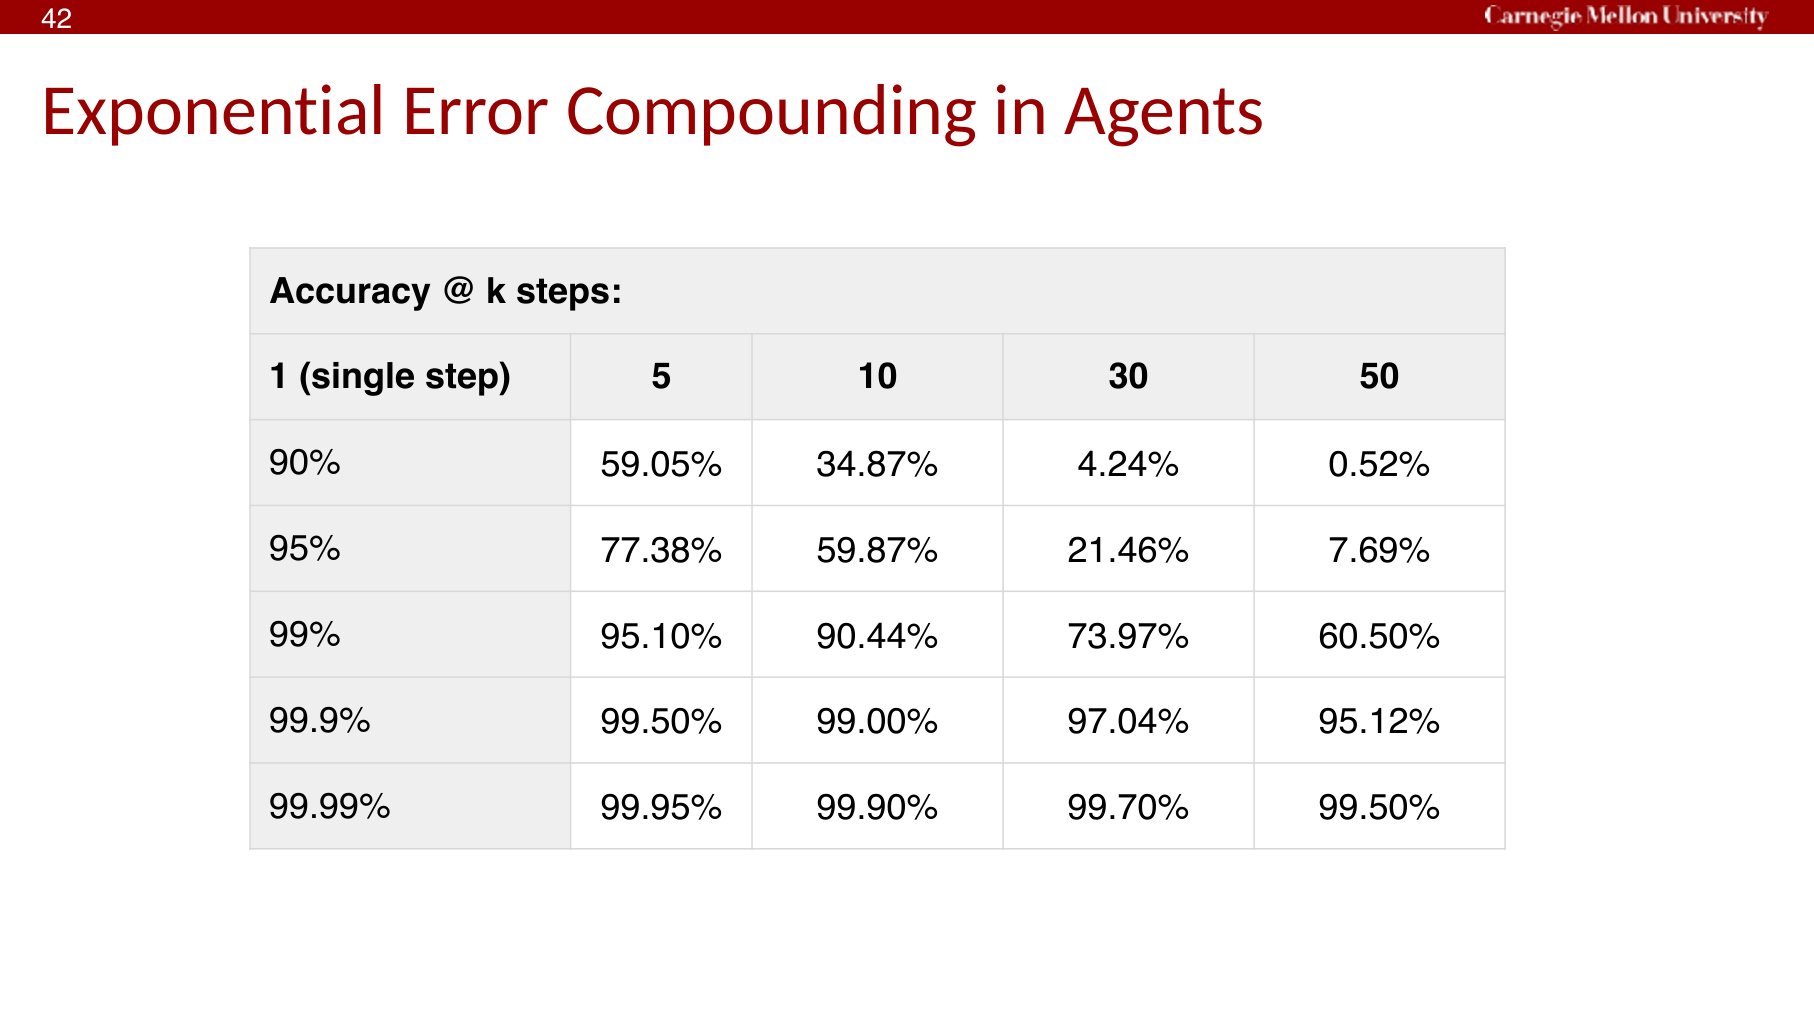
\includegraphics[width=0.74\textwidth]{../lectures/lec06_multimodal_autonomous_agents/figures/lec06_fig_005.png}
\caption{长程任务中的误差累积：即使单步准确率尚可，整条 trajectory 的成功率也会快速下降。}
\end{figure}

这一页最值得教材化展开的地方在于，讲者并不是在说“模型还不够强”，而是在说 \textbf{autonomous agents 的误差结构和单轮问答完全不同}。如果把每一步大致视作正确率为 $p$ 的决策，那么长程任务近似成功率会像
\[
\Pr(\text{success at }k\text{ steps}) \approx p^k
\]
那样快速下降。这里 $p$ 是近似单步正确率，$k$ 是必须连续做对的交互步数。这个公式并不追求严格统计精确，而是帮助读者抓住本讲的核心直觉：\textbf{local decisions have global consequences}。

因此，单纯 repeated sampling 并不能根治问题。你可以多采几条完整 trajectory，但搜索空间是指数大的，而且如果没有对 \emph{中间状态} 的判断能力，系统很难知道什么时候该继续扩展、什么时候该 backtrack。

\subsection{Tree Search for Language Model Agents}

\begin{figure}[H]
\centering
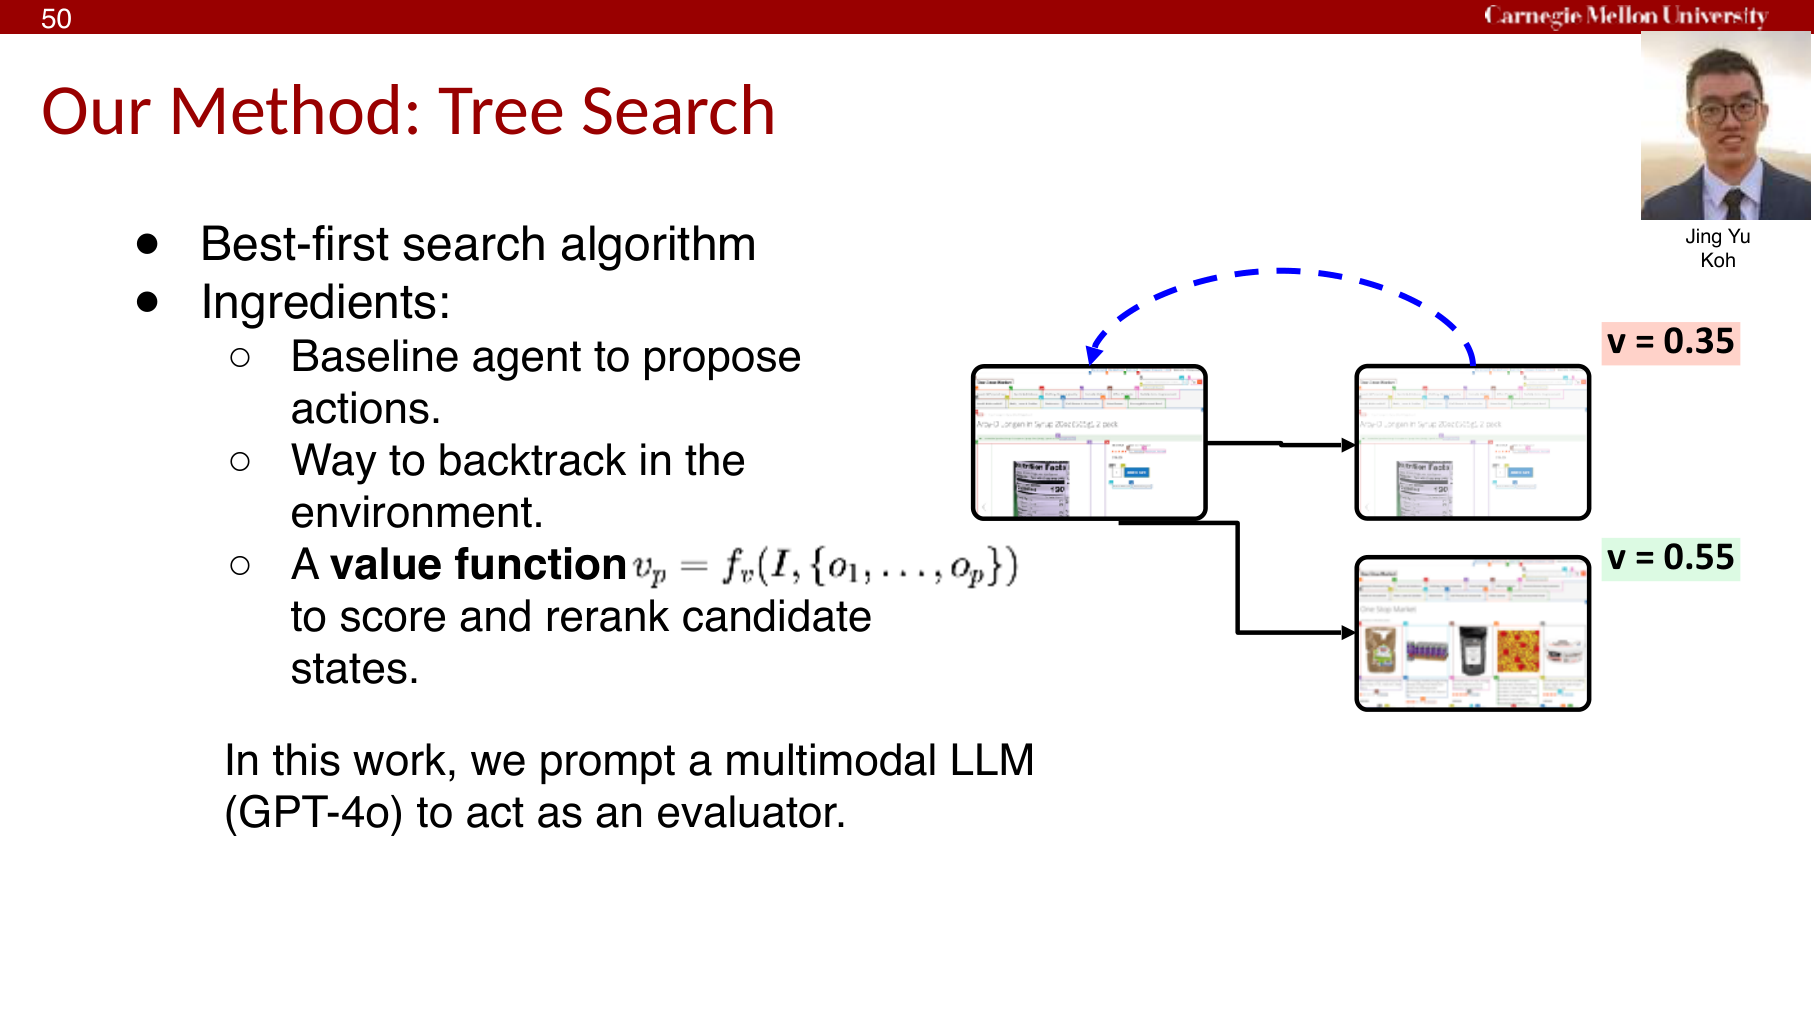
\includegraphics[width=0.76\textwidth]{../lectures/lec06_multimodal_autonomous_agents/figures/lec06_fig_006.png}
\caption{Tree Search 的核心 ingredients：baseline policy 负责提议分支，value function 负责评估中间状态。}
\end{figure}

这正是 \textbf{Tree Search for Language Model Agents} 的出发点。它的基本想法是：不要把 agent 当成只能沿一条 trajectory 前进的策略，而要把它当成一个能提出候选 action branches 的 proposal model；然后再配一个 \textbf{value function} 去评估中间状态的潜力。一个简化写法是：
\[
\hat{s}_t = \arg\max_{s \in \mathcal{F}_t} v_\phi(s),\qquad \mathcal{F}_{t+1}=\operatorname{Expand}(\hat{s}_t; b,d,c).
\]
这里 $\mathcal{F}_t$ 是当前 frontier，$v_\phi(s)$ 是中间状态评分函数，$b,d,c$ 分别控制 branching factor、search depth 与总 budget。直觉上，它做的是“在有限预算下，优先把算力用在最有希望的 partial trajectories 上”。

\begin{lstlisting}
initialize frontier with current state
while budget remains:
    pop highest-value state
    if value exceeds threshold: commit
    expand candidate actions from baseline agent
    evaluate children with value function
return best state found
\end{lstlisting}

这个算法与 L01 中讲到的 test-time search 形成了直接呼应。区别在于，这里 search 的对象不是思维链节点，而是 \textbf{真实环境中的交互状态}。因此它不仅要考虑 reasoning quality，还要考虑页面回退、环境恢复和 backtracking 成本。

\subsection{实验结论、compute tradeoff 与局限性}

\begin{figure}[H]
\centering
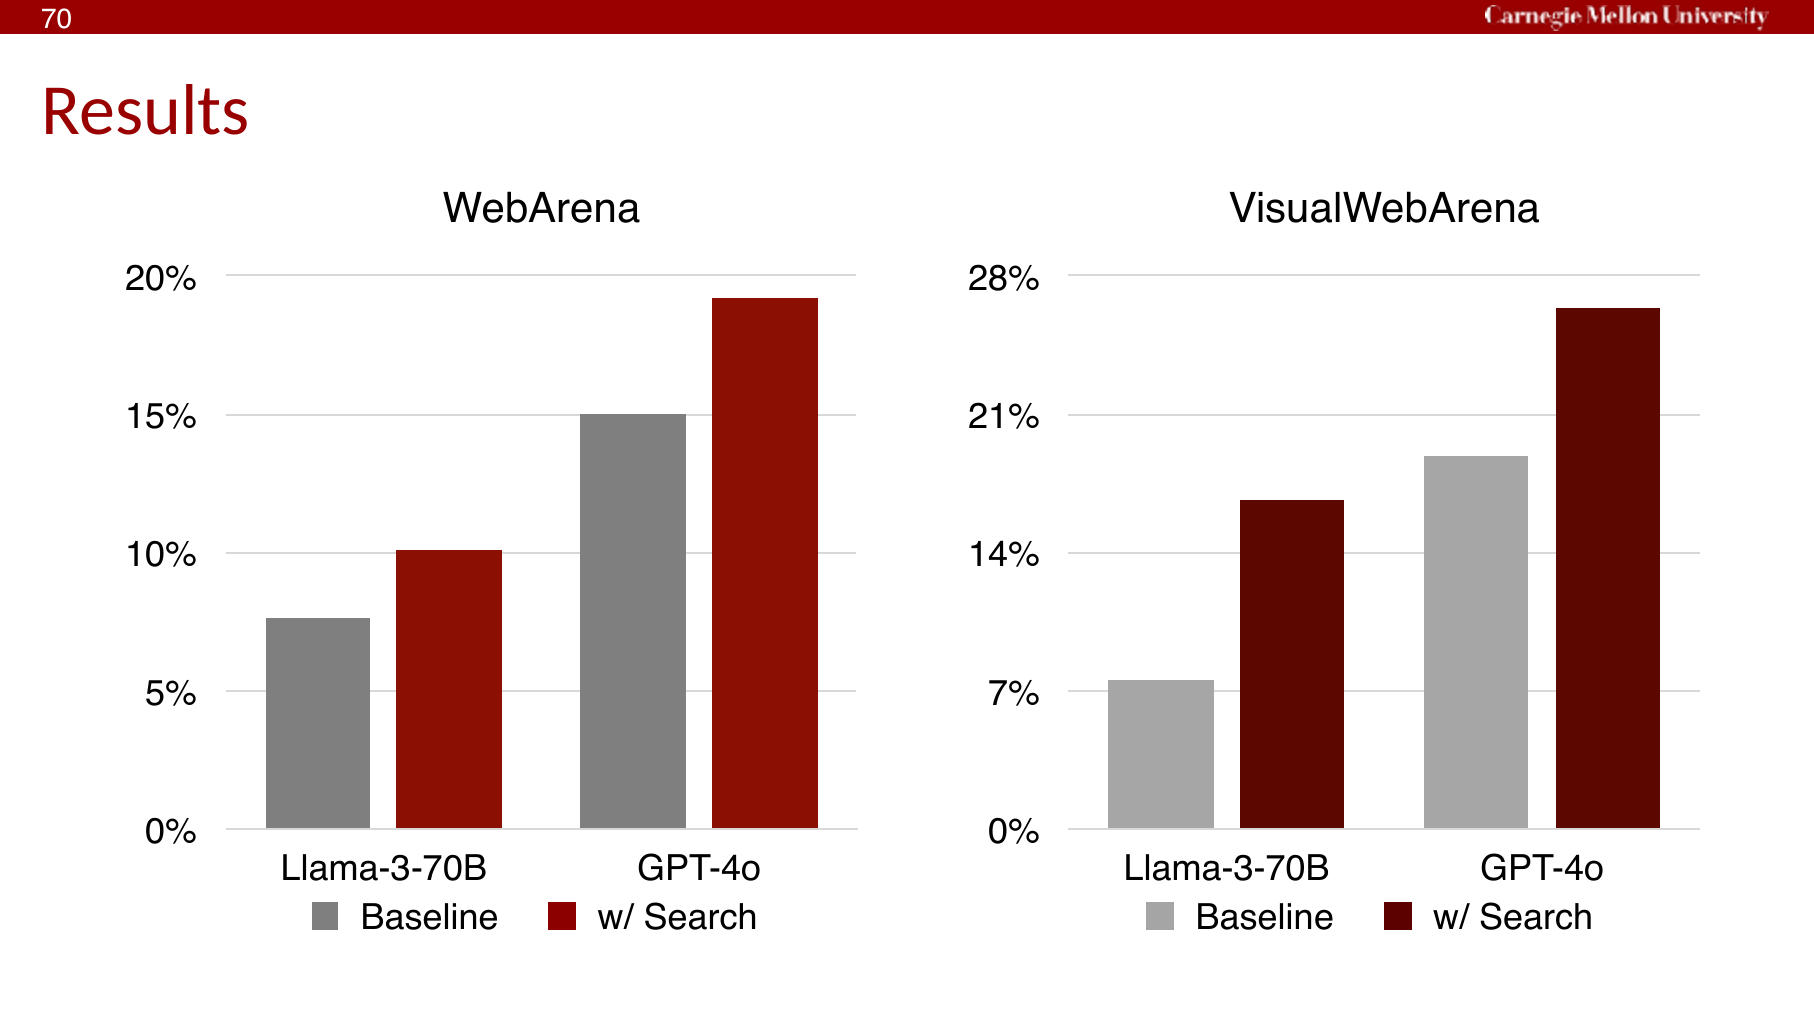
\includegraphics[width=0.76\textwidth]{../lectures/lec06_multimodal_autonomous_agents/figures/lec06_fig_007.png}
\caption{Search 可以显著提高 success rate，但与 human performance 仍有巨大差距。}
\end{figure}

讲者给出的结果很重要，因为它同时包含 \textbf{正面结论} 和 \textbf{系统局限}。

正面结论是：在 VisualWebArena 和 WebArena 上，把 search 加到 baseline GPT-4o agent 上，成功率会有显著提升。项目页也明确指出，VisualWebArena 上相对提升接近 40\%，并且随着 search budget 增加，表现一般会继续上升。这说明 \textbf{inference-time compute 在 realistic web agents 上是真正有效的设计变量}。

局限性同样清楚：
\begin{itemize}
\item search 很慢，因为回溯到旧状态在现实网页环境中代价高。
\item 结果高度依赖 value function 质量；若 value model 不会判断中间状态是否有前景，search 只会更昂贵地走错路。
\item baseline policy 太弱时，frontier 里本来就没有好分支，search 的上限也会受限。
\end{itemize}

因此，讲者后来把当前工作概括为三条方向：把 search 当成 policy improvement operator、微调更强的 value function、并系统研究 baseline agent 与 search budget 的 compute tradeoff。这一点与 L01 的 reasoning-time scaling 视角完全一致。

\section{Agents Suffer From A Data Problem}

\subsection{为什么 agent training 特别缺数据}

本讲中最值得注意的一句判断是：\textbf{agents suffer from a data problem}。原因很直接。LLM 可以从大规模现成文本中预训练，但 GUI 或 web agents 所需的不是普通文本，而是带有环境状态、操作步骤和完成判定的 trajectory data。人工标注这种数据非常贵，而且可扩展性极差。

这意味着很多今天的 agent 实践其实是：\textbf{先离线训练一个模型，再在几乎没有针对性 agent 经验的数据分布上 zero-shot 部署。} 这样做当然能跑出 demo，但遇到真实 benchmark 时很快会暴露出规划、state tracking 和 grounding 的不足。

\subsection{InSTA：用 synthetic tasks 扩大训练分布}

讲者随后介绍 \textbf{Towards Internet-Scale Training For Agents (InSTA)}。其目标不是凭空“合成一点数据”，而是把互联网本身变成 task source，再用模型生成、筛选、验证 agentic tasks，从而把训练分布扩展到更大范围的网站。

\begin{figure}[H]
\centering
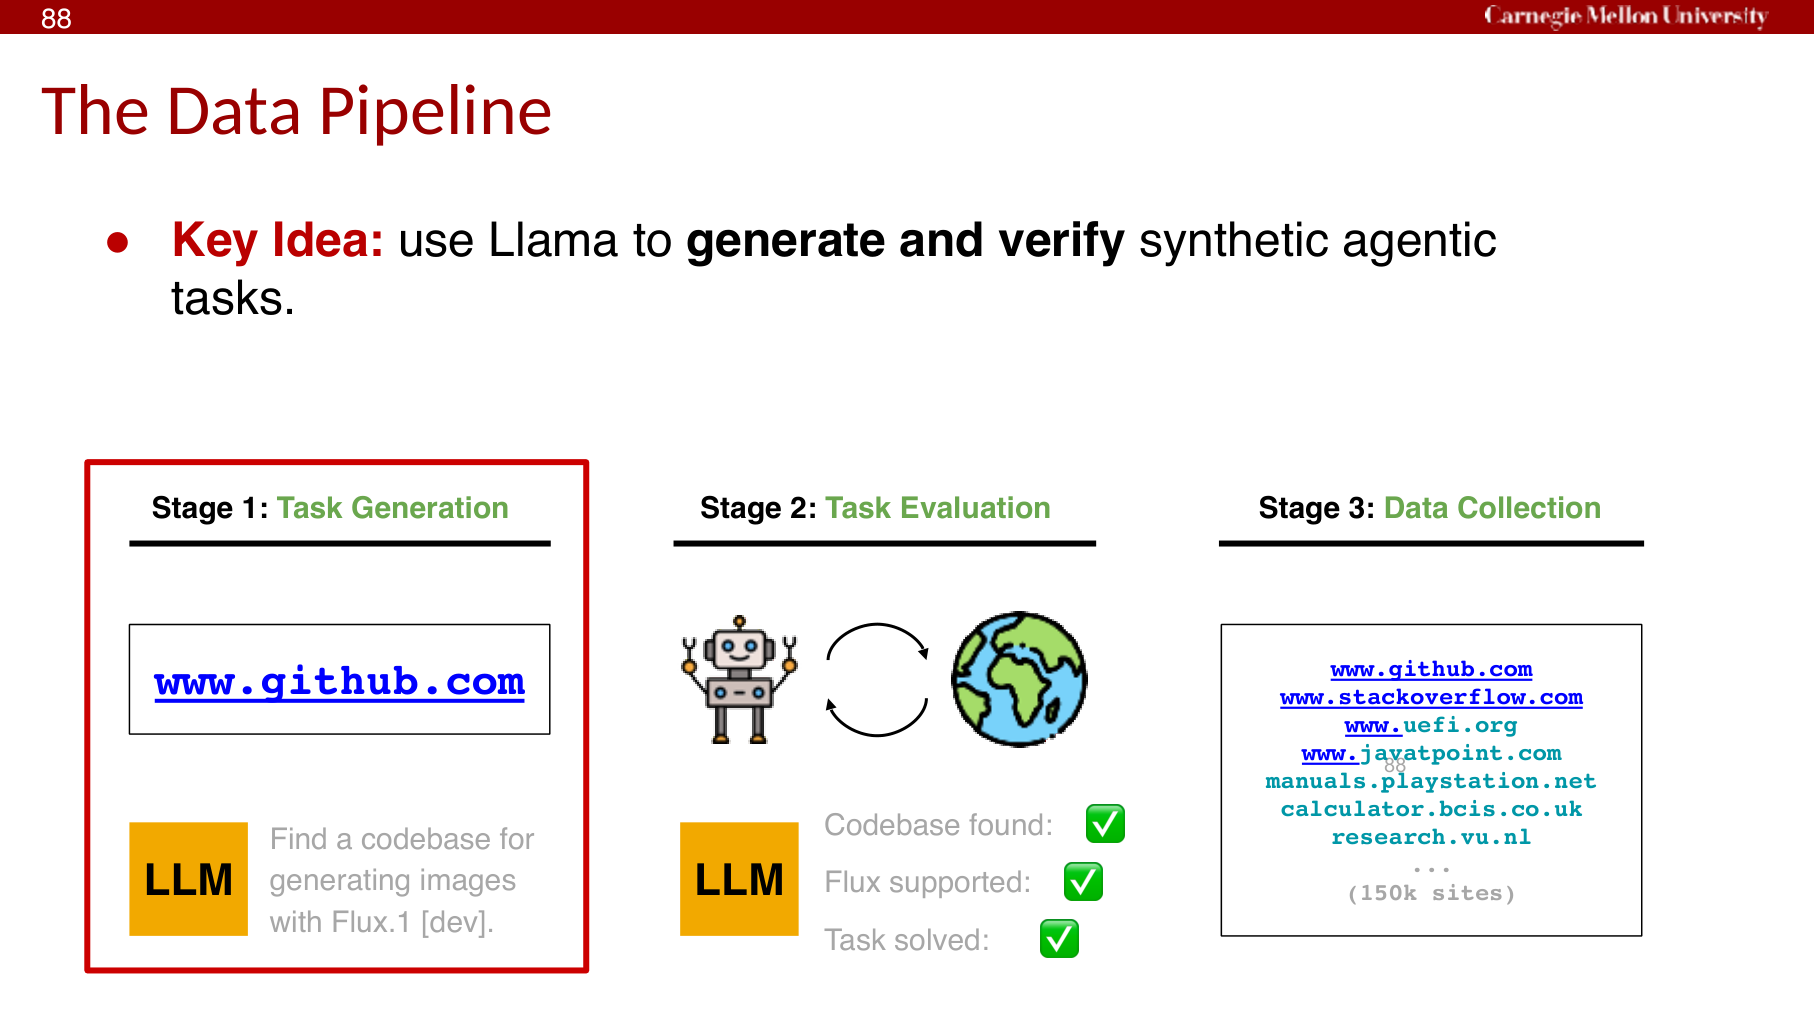
\includegraphics[width=0.78\textwidth]{../lectures/lec06_multimodal_autonomous_agents/figures/lec06_fig_008.png}
\caption{InSTA 的管线：从 web domains 生成 realistic tasks，再做验证与扩展。}
\end{figure}

其基本循环可以写成：
\begin{lstlisting}
sample a web domain
use Llama to propose realistic tasks
run/inspect trajectories
estimate task success with verifier
keep feasible and solvable tasks for large-scale training
\end{lstlisting}

这一步与静态 instruction generation 的区别在于，生成出来的任务要能 \textbf{被 agent 真正在环境中执行和验证}。也就是说，task generation 必须与 task verification 配对。

\begin{figure}[H]
\centering
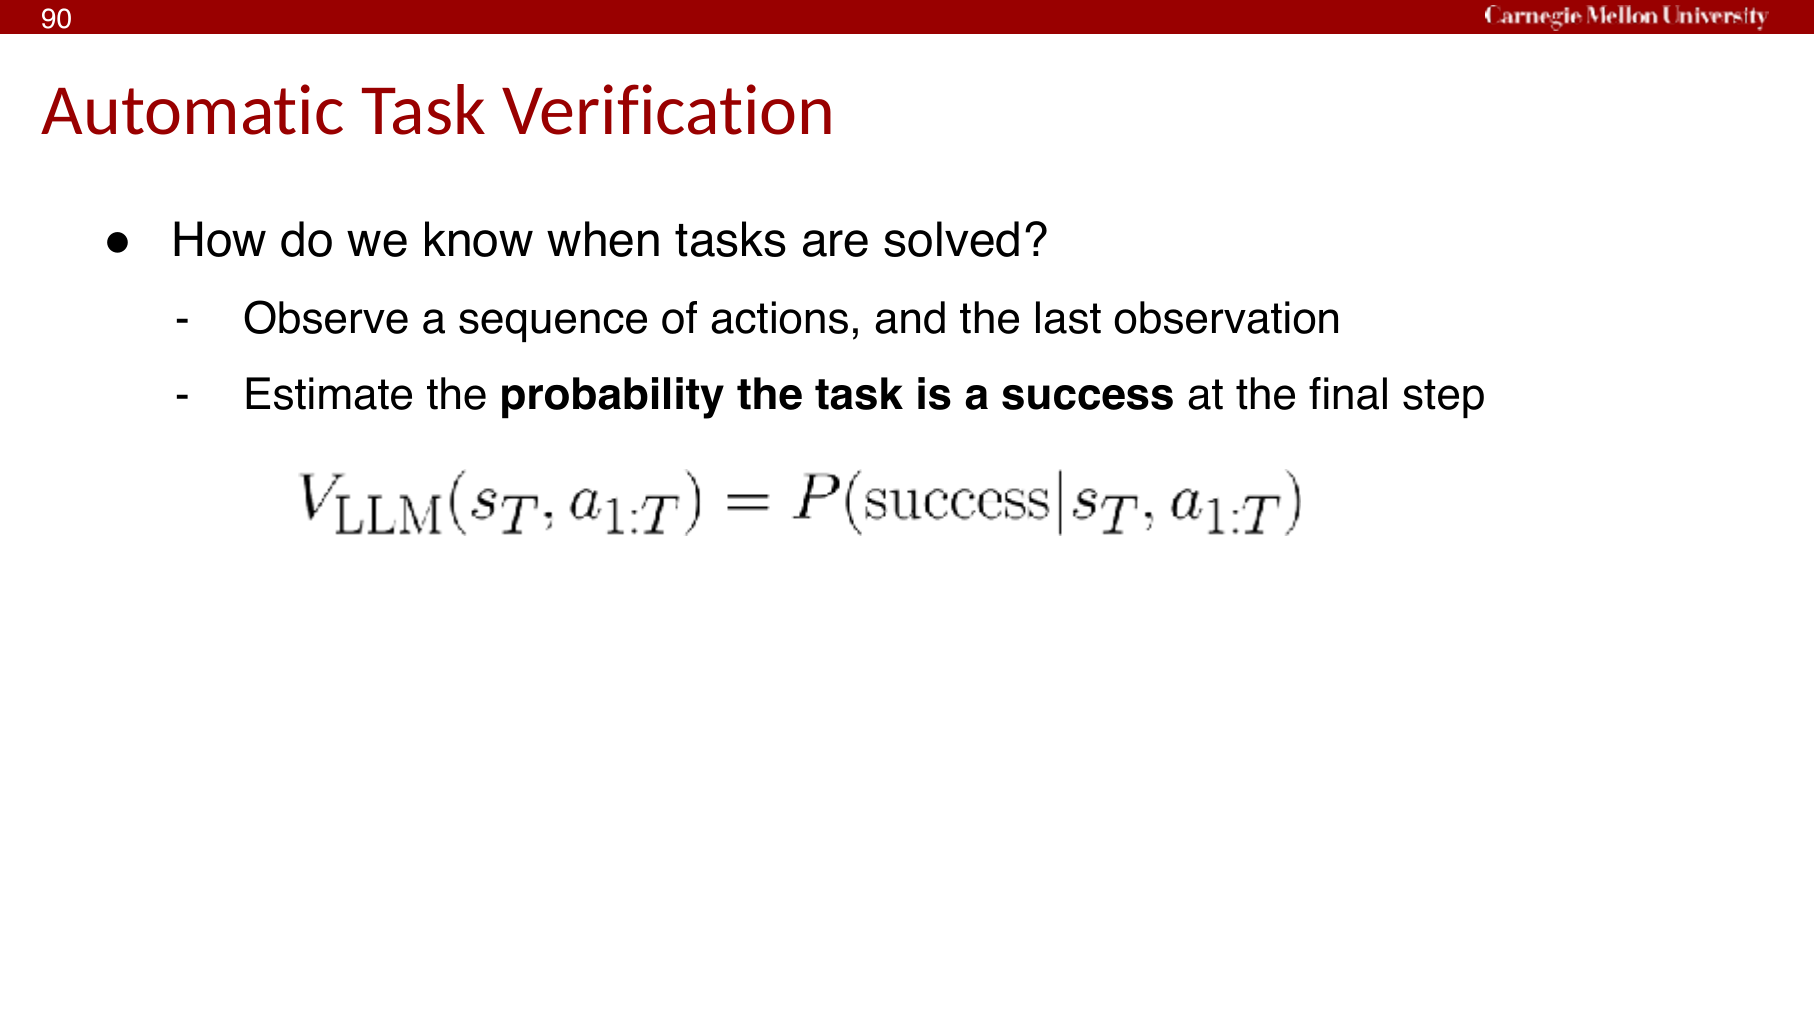
\includegraphics[width=0.78\textwidth]{../lectures/lec06_multimodal_autonomous_agents/figures/lec06_fig_009.png}
\caption{Automatic task verification：观察轨迹与最终状态，估计任务是否真正成功。}
\end{figure}

教材化看，这里的核心不是某个具体 Llama prompt，而是：\textbf{agent data pipeline 必须同时回答“任务是什么”“怎么知道做成了”“怎么扩大规模”三个问题。} 如果只会生成 instruction，而不会验证任务完成，那么最终只是在制造噪声 supervision。

\begin{warningbox}{为什么 synthetic data 不是万能药}
Synthetic tasks 可以扩展覆盖面，但并不会自动保证 realism、safety 或 distribution match。生成出来的任务也可能偏向信息检索、回避状态修改、或隐含不安全网站。lecture slides 提到的 filtering 和 feasibility checks，正是在防止这种漂移。
\end{warningbox}

\section{从 Web Agents 到 Physical Agents}

\subsection{Perception-action loop 在机器人里更严苛}

讲者最后把视角从网页转向 physical agents。这个转向很重要，因为它说明本讲不是一组离散 case studies，而是在强调一种更一般的 multimodal autonomy 框架：\textbf{感知、规划、状态估计、动作执行与反馈修正的闭环。}

\begin{figure}[H]
\centering
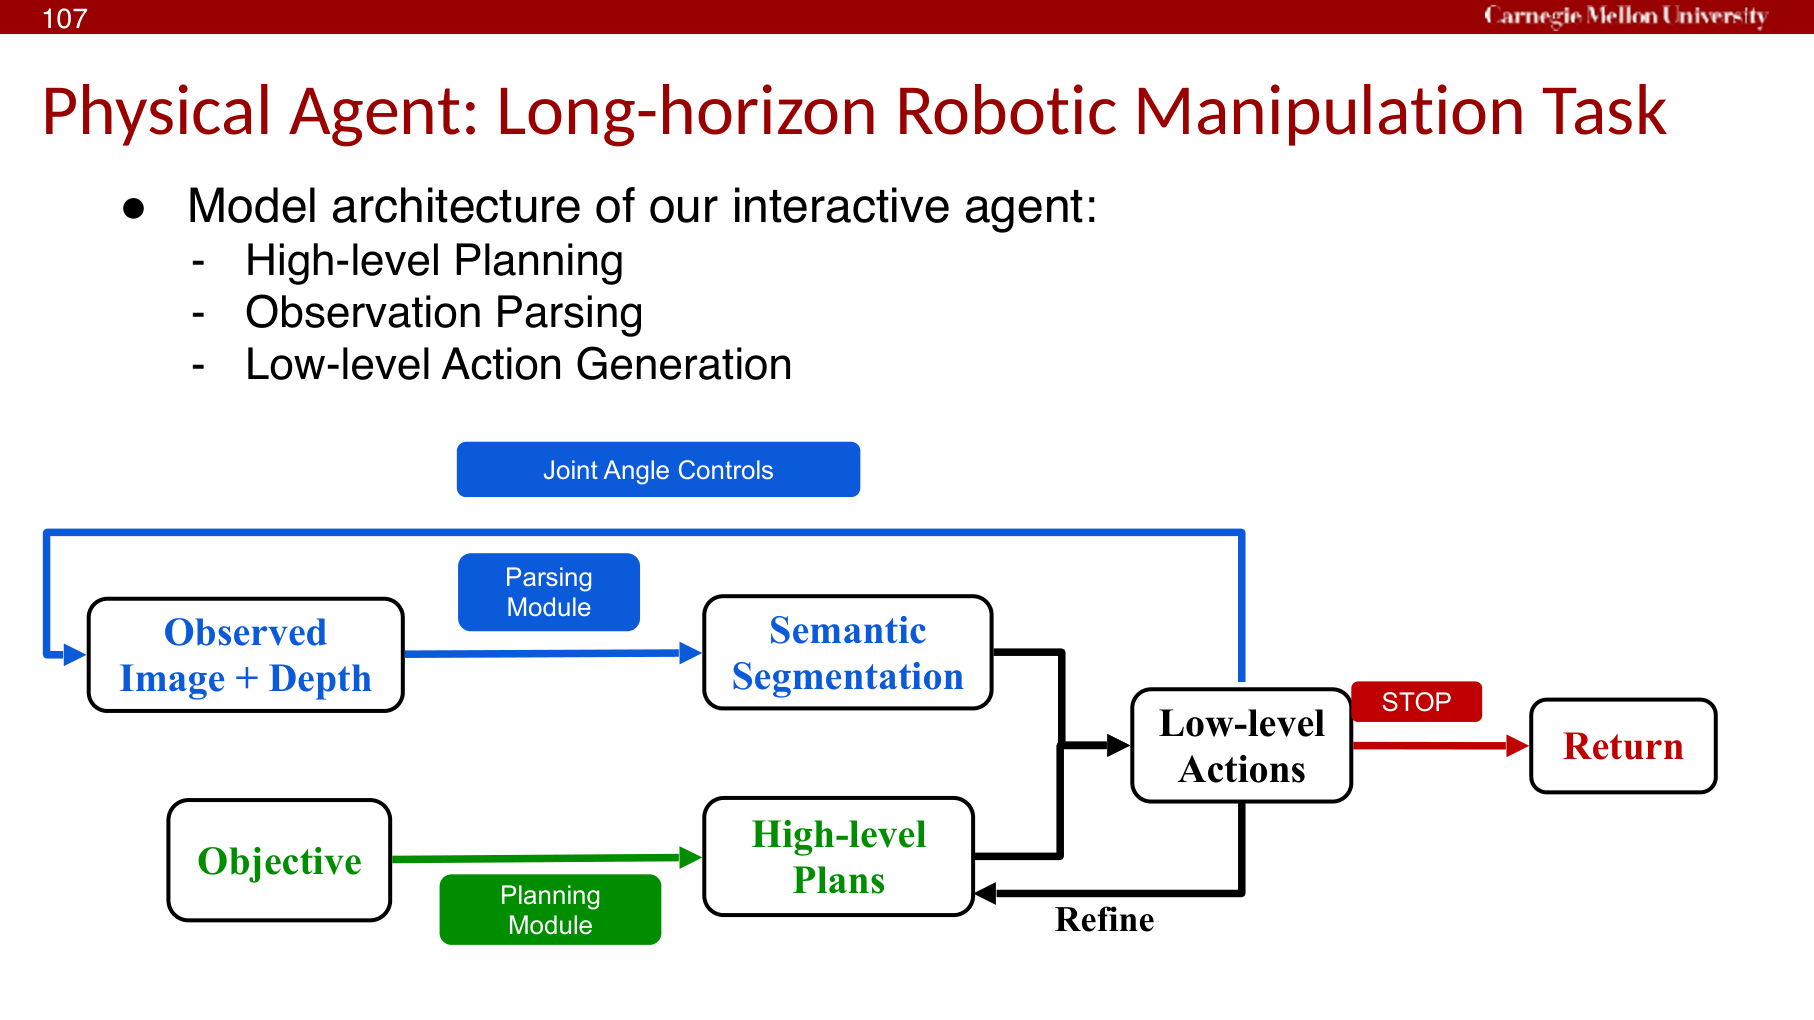
\includegraphics[width=0.80\textwidth]{../lectures/lec06_multimodal_autonomous_agents/figures/lec06_fig_010.png}
\caption{Physical agent 的输入包括 image、depth 和 semantic segmentation，因而比 web agent 更接近 embodied autonomy。}
\end{figure}

与 web agents 相比，physical agents 至少多了三层难度：
\begin{itemize}
\item 视觉误差会直接传导到物理执行误差。
\item 环境状态恢复成本更高，错误动作代价更大。
\item 成功往往要依赖多个连续子任务都完成，因此长程成功率更加脆弱。
\end{itemize}

\subsection{Plan-Seq-Learn：分层解决 long-horizon manipulation}

\begin{figure}[H]
\centering
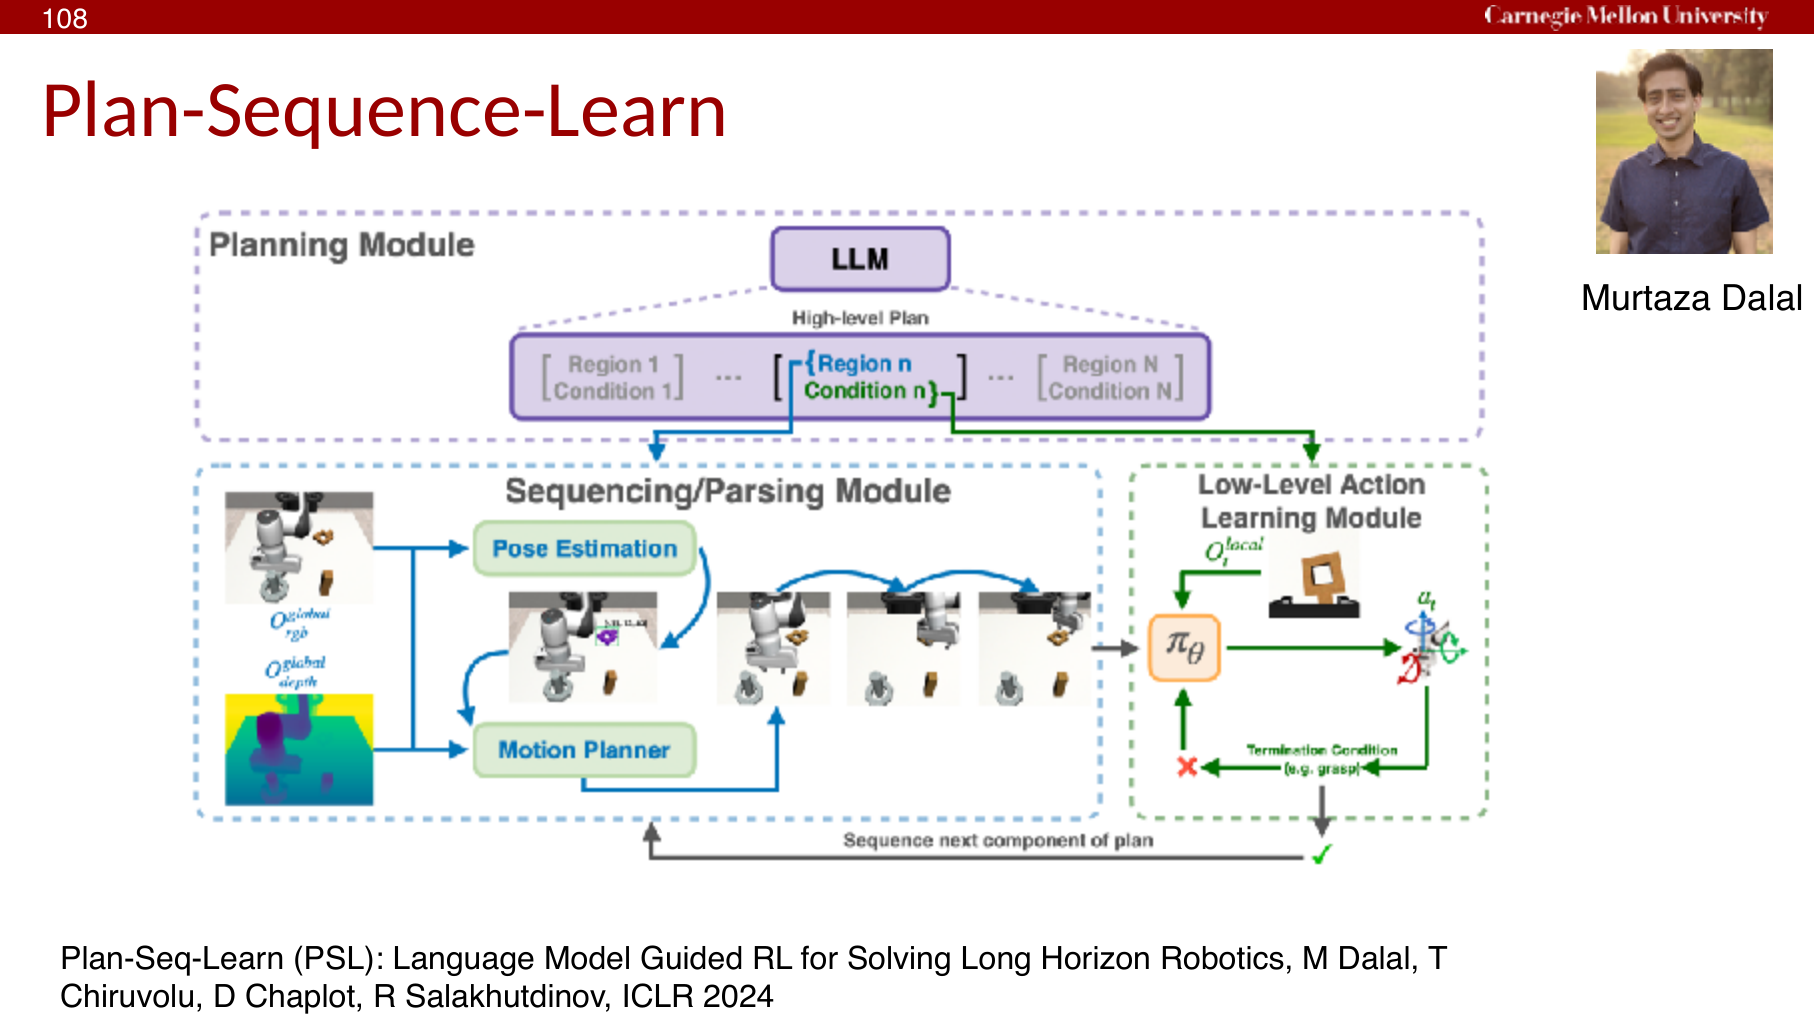
\includegraphics[width=0.82\textwidth]{../lectures/lec06_multimodal_autonomous_agents/figures/lec06_fig_011.png}
\caption{Plan-Seq-Learn 用语言规划、scene grounding 和局部 RL control 分层处理 manipulation。}
\end{figure}

Plan-Seq-Learn 的核心不是把一个大模型直接端到端映射到所有控制信号，而是先把任务拆成可管理的层级。slides 明确给出 manipulation 成功率可写成：
\[
P(\mathrm{success}) = P(\mathrm{task}_1) \cdot P(\mathrm{task}_2\mid \mathrm{task}_1) \cdots P(\mathrm{task}_n\mid \mathrm{task}_{<n}).
\]
其中每个 $\mathrm{task}_i$ 是一个子目标或阶段。这个公式的直觉与 error compounding 完全一致：如果每一步都只有中等成功率，那么整体 success 会迅速坍缩。因此系统必须：
\begin{itemize}
\item 用 \textbf{language planner} 生成结构化的高层子目标。
\item 用 \textbf{sequencing / parsing module} 把语言子目标对齐到当前场景中的对象与条件。
\item 用 \textbf{local RL controller} 学习低层 interaction policies，而不是为每个阶段单独写控制器。
\end{itemize}

\begin{lstlisting}
language planner proposes structured subgoals
sequencing module grounds each subgoal in the scene
local RL controller executes low-level actions
feedback updates the next subgoal execution
\end{lstlisting}

这种设计的意义在于：它把高层 reasoning、环境 grounding 和 motor control 分开，使每层都能利用更合适的 inductive bias。它也揭示出与 GUI agents 的共性：\textbf{不是所有多模态 agent 都应该追求一个“单模型一步到位”的方案。}

\section{Readings 与跨讲联系}

本讲的 readings 形成一条清晰链条。\textbf{Mind2Web} 说明真实网站数据的分布与离线行为建模难题；\textbf{WebArena} 把问题升级为可交互、可复现、execution-based 的现实环境；\textbf{VisualWebArena} 证明视觉 grounding 必须进入 benchmark；\textbf{Tree Search for Language Model Agents} 则说明 inference-time compute 可以直接改变 realistic web tasks 上的 success rate。

与 L01 的关系尤其直接。L01 主要讨论在 reasoning task 上如何把 test-time compute 分配给更长、更宽、更可验证的 search 过程；本讲则把同样的思想搬到了 \textbf{真实环境中的 multimodal agents}：候选不再只是 reasoning trace，而是环境状态与动作序列。下一讲如果继续推进 GUI/OS agents，这里的 benchmark distinction、grounding 问题与 data bottleneck 都会成为前提。

\section{本章小结}

\begin{figure}[H]
\centering
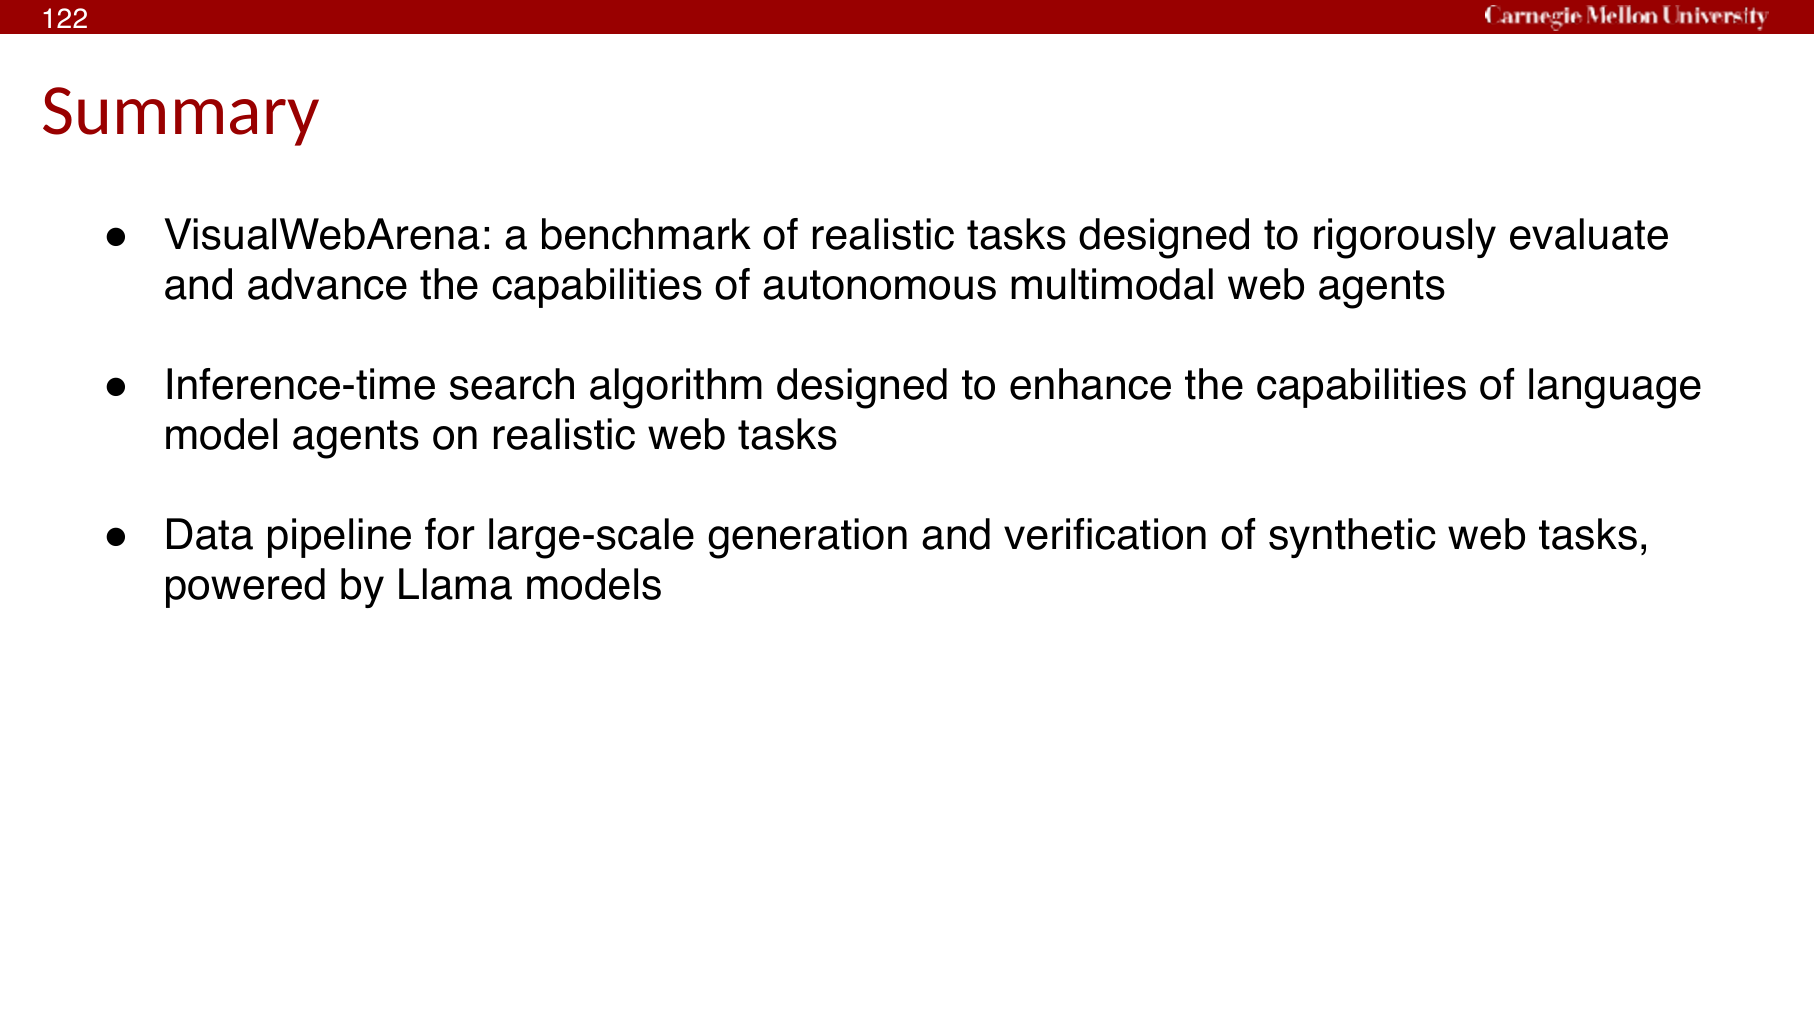
\includegraphics[width=0.80\textwidth]{../lectures/lec06_multimodal_autonomous_agents/figures/lec06_fig_012.png}
\caption{本讲最终把 benchmark、search、synthetic data 和 robotics 串成一条多模态 autonomy 主线。}
\end{figure}

本讲最重要的结论可以压缩成四句：
\begin{enumerate}
\item 对真实 web agents 来说，\textbf{benchmark realism} 是第一性问题；没有 environment，很多错误无法被 functional correctness 揭示。
\item 视觉 grounding 不是“加一点图像输入”，而是网页任务语义本身的一部分，因此 \textbf{VisualWebArena} 这类 benchmark 不可替代。
\item \textbf{Tree search} 证明 inference-time compute 对 multimodal agents 同样有效，但它高度依赖 value function 质量和系统预算。
\item 无论是 web agents 还是 physical agents，最终都绕不开 \textbf{data pipeline、grounding quality、long-horizon planning} 三个系统瓶颈。
\end{enumerate}

\section{复习题}
\begin{enumerate}
\item 用自己的话区分 Mind2Web、WebArena 和 VisualWebArena 的主要目标。
\item 为什么讲者说 HTML-only representation 对真实网页任务不够？
\item Tree search 为什么需要 value function，而不是只做 repeated sampling？
\item InSTA 的 automatic verification 在数据管线里起什么作用？
\item 为什么 physical agents 比 web agents 更强调 perception-action loop 的稳定性？
\end{enumerate}

\section{深入思考题}
\begin{enumerate}
\item 如果你只能改进 baseline agent、value function、search budget 三者之一，你会优先改哪个？为什么？
\item 对网页 agent 来说，视觉 grounding 与长程规划哪个是更基础的瓶颈？请给出任务依赖的回答。
\item Plan-Seq-Learn 这种分层结构是否会限制端到端性能上限？在什么情况下它反而是必要的？
\end{enumerate}

\section{延伸阅读}
\begin{itemize}
\item Mind2Web: Towards a Generalist Agent for the Web.
\item WebArena: A Realistic Web Environment for Building Autonomous Agents.
\item VisualWebArena: Evaluating Multimodal Agents on Realistic Visual Web Tasks.
\item Tree Search for Language Model Agents.
\item Plan-Seq-Learn: Language Model Guided RL for Long-Horizon Robotics.
\end{itemize}

\input{chapters/lec07_multimodal_agents_perception_to_action.tex}
\part{Formal Mathematics, Verification, and Theorem Proving}
\input{chapters/lec08_alphaproof_formal_mathematics.tex}
\input{chapters/lec09_autoformalization_theorem_proving.tex}
\input{chapters/lec10_advanced_theorem_proving.tex}
\part{Abstraction, Discovery, Safety, and Security}
\input{chapters/lec11_abstraction_discovery_llm_agents.tex}
\input{chapters/lec12_safe_secure_agentic_ai.tex}
\appendix
\chapter{练习与思考题附录}

本附录按章节组织全书练习，目标不是提供机械性题库，而是把每章最重要的概念边界、方法权衡、环境反馈、失败模式与延伸阅读系统化下来。每章都包含三类任务：
\begin{itemize}
\item 概念复习题：检查读者是否真正掌握术语、定义和结构关系。
\item 深入思考题：要求读者比较方法假设、分析边界条件或提出替代设计。
\item 实践与阅读题：要求读者实现最小系统、设计 evaluator、或结合论文进一步抽象。
\end{itemize}
其中 theorem proving 相关章节额外加入形式化与证明题，coding/security 相关章节额外加入 failure analysis 或 safety analysis 题。

\section{第 1 章：推理时计算（Inference-Time Techniques for LLM Reasoning）}

\subsection*{概念复习题}
\begin{enumerate}
\item 为什么 CoT 的价值不只是“让答案更长”，而是重新分配 inference-time compute？
\item Analogical Prompting 与 few-shot CoT 的 inductive bias 有何不同？
\item OPRO 为什么可以被视为 prompt engineering 的 optimization loop？
\item Self-Consistency 为什么依赖多样化采样，而不是重复同一条推理链？
\item Outcome Reward Model 与 Process Reward Model 分别适合什么类型的搜索控制？
\end{enumerate}

\subsection*{深入思考题}
\begin{enumerate}
\item 如果 verifier 只对最终答案可靠、对中间状态不可靠，Tree of Thoughts 会怎样偏离正确搜索？
\item 为什么没有外部反馈时，self-correction 可能只是“更自信地重复错误”？
\item 对开放式长文本写作、策略规划或法律分析任务，你会如何构造足够可靠的反馈器？
\end{enumerate}

\subsection*{实践与阅读题}
\begin{enumerate}
\item 在数学问答任务上实现 Self-Consistency，对比 sample budget 从 $1, 4, 8, 16$ 时的性能与成本。
\item 在代码生成任务上实现最小版 self-debugging loop，比较“纯文本反思”与“执行反馈反思”的修复率差异。
\item 阅读本章核心论文后，写一段短文比较 reranking、tree search、verifier-guided repair 三者对 agent workflow 的不同影响。
\end{enumerate}

\subsection*{形式化与证明题}
\begin{enumerate}
\item 把 verifier ranking 写成有限候选集上的最优化问题，并说明步骤级评分为何会改变搜索策略。
\item 讨论 theorem proving 场景中，为什么 partial-state evaluation 往往比 final-answer reranking 更重要。
\end{enumerate}

\subsection*{Failure Analysis}
\begin{enumerate}
\item 如果 self-correction 的反馈来自同分布 LLM 而不是真实环境，这个系统会出现哪些共偏差风险？
\item 对代码 agent 而言，execution consistency 与真实安全性之间存在哪些结构性错位？
\end{enumerate}

\section{第 2 章：学习推理（Learning to Reason with LLMs）}

\subsection*{概念复习题}
\begin{enumerate}
\item 为什么可以把 DPO 视为本章中的 optimizer primitive，而不是完整 recipe？
\item Self-Rewarding 与标准 RLHF 的根本差异是什么？
\item CoVe 如何用 verification-oriented prompting 降低 hallucination？
\item IRPO 为什么依赖 verifiable final answers？
\item Meta-Rewarding / EvalPlanner 为什么把 judgment 本身当作训练对象？
\end{enumerate}

\subsection*{深入思考题}
\begin{enumerate}
\item 如果 actor 与 judge 共享同一个基座模型，它们之间会形成哪些共偏差与 shortcut？
\item 在开放式 agent 任务里，哪类环境反馈能替代人工 preference，哪类却不能？
\item EvalPlanner 的思想怎样迁移到代码审查、实验设计或安全审计任务？
\end{enumerate}

\subsection*{实践与阅读题}
\begin{enumerate}
\item 用一个小型 QA 数据集实现 CoVe 四步流程，并报告 hallucination rate 的变化。
\item 构造一个具有可验证 final answer 的推理任务，手工模拟 IRPO 的 preference-pair 生成过程。
\item 选读 Self-Rewarding 或 Meta-Rewarding 论文，分析“训练更强的 judge”与“训练更强的 actor”哪一个更像本章主线。
\end{enumerate}

\section{第 3 章：推理、记忆与规划（Reasoning, Memory, and Planning of Language Agents）}

\subsection*{概念复习题}
\begin{enumerate}
\item 什么是 language agent，它与普通 LLM application 的本质区别是什么？
\item HippoRAG 试图修复现有 RAG 的哪个结构缺陷？
\item 为什么 implicit reasoning 不等于“没有推理”？
\item reactive policy、tree search、model-based planning 分别适合什么任务结构？
\item WebDreamer 中的 world model 承担什么角色？
\end{enumerate}

\subsection*{深入思考题}
\begin{enumerate}
\item 对长期在线运行的 agent，memory update 如何同时避免 catastrophic forgetting 与 privacy leakage？
\item grokking 的 insight 能否转化为更强的 agent foundation model 训练原则？
\item world-model planning 是否可能放大模型幻觉？你会如何设计 guardrail？
\end{enumerate}

\subsection*{实践与阅读题}
\begin{enumerate}
\item 为一个简单网页任务分别实现 reactive policy 与 model-based policy，对比交互次数、成功率和错误恢复能力。
\item 设计一个多跳记忆问答案例，比较 dense retrieval 与图扩散检索的差异。
\item 结合 HippoRAG、Grokked Transformers 与 WebDreamer，写一段短评说明为什么“memory / reasoning / planning”应被视为统一能力图谱。
\end{enumerate}

\section{第 4 章：推理模型的开放训练配方（Open Training Recipes for Reasoning in Language Models）}

\subsection*{概念复习题}
\begin{enumerate}
\item 为什么“开放”本身是 training recipe 的一部分，而不只是社区治理议题？
\item SFT、preference tuning、RLVR 各自优化什么对象？
\item 为什么 reasoning data 往往需要 chain-of-thought，而不能只保留 final answer？
\item DPO 相比 PPO 省掉了哪些组件？这会带来什么代价？
\item RLVR 为什么只在特定任务结构上特别有效？
\end{enumerate}

\subsection*{深入思考题}
\begin{enumerate}
\item 当 post-training 预算极低时，你会优先投资更好的 preference data 还是更复杂的优化算法？说明理由。
\item 为什么 budget forcing 在某些任务上有效，在另一些任务上只是延长错误推理？
\item OpenScholar 为什么能够体现 open recipe 的 downstream 价值？
\end{enumerate}

\subsection*{实践与阅读题}
\begin{enumerate}
\item 为一个数学 reasoning 模型设计 data-mixing plan，明确写出数据来源、过滤策略与 evaluator。
\item 为一个有 gold answer 的任务写出 verifier 接口，并分析它可能被 reward hacking 的方式。
\item 选读本章任一 reading，写一页备忘录比较 open recipe 与 closed recipe 在 reproducibility 和 failure diagnosis 上的差异。
\end{enumerate}

\section{第 5 章：Coding Agents 与漏洞检测（Coding Agents and AI for Vulnerability Detection）}

\subsection*{概念复习题}
\begin{enumerate}
\item coding agent 与普通 code completion 的本质区别是什么？
\item 为什么本章先讲 evaluator 再讲 architecture？
\item ReAct、Agentless、AutoCodeRover 在 control flow 上分别体现了什么设计取向？
\item 为什么 CTF / security task 对工具接口和环境反馈的要求更高？
\item Big Sleep 为什么强调 variant analysis，而不是开放式漏洞猎取？
\end{enumerate}

\subsection*{深入思考题}
\begin{enumerate}
\item 在什么条件下，procedural agent 会优于 dynamic agent？
\item 如果 benchmark 泄漏或覆盖不足，pass@k 与 SWE-Bench 风格指标会如何误导系统设计？
\item 为什么“能生成 exploit 思路”不等于“能稳定做安全研究”？
\end{enumerate}

\subsection*{实践与阅读题}
\begin{enumerate}
\item 为一个仓库级 bug-fixing agent 设计最小 tool palette，并说明每个工具的反馈形式。
\item 为 security agent 设计 sandbox 与 logging policy，标出哪些操作必须被限制、审批或留痕。
\item 给 Big Sleep 风格的 variant-analysis workflow 设计 verifier，并说明如何降低误报。
\end{enumerate}

\subsection*{Failure Analysis / Safety Analysis}
\begin{enumerate}
\item 对一个具备 shell、network、browser、git 权限的 coding agent，做一份 capability-risk matrix，分析高风险组合。
\item 设计一个 failure review 模板，用来区分 benchmark overfitting、tool misuse、environment mismatch 与真实安全缺陷。
\end{enumerate}

\section{第 6 章：多模态自主体（Multimodal Autonomous AI Agents）}

\subsection*{概念复习题}
\begin{enumerate}
\item 为什么 Mind2Web、WebArena 与 VisualWebArena 不能互相替代？
\item HTML-only representation 为什么会在真实网页任务中失真？
\item VisualWebArena 的 visually grounded evaluation 解决了什么关键问题？
\item 长程 agent 任务为什么会出现 exponential error compounding？
\item Tree search 相比 repeated sampling 的主要优势是什么？
\item 为什么 value function 的质量会直接限制 search gain？
\item InSTA 为什么强调 task generation 与 task verification 两阶段？
\item 为什么 synthetic tasks 能缓解 data bottleneck，却不能自动解决 realism 与 safety？
\end{enumerate}

\subsection*{深入思考题}
\begin{enumerate}
\item 如果一个 agent 在 WebArena 上表现好、在 VisualWebArena 上表现差，你会首先怀疑它缺什么能力？
\item 在固定预算下，你会优先提升 baseline policy、value function，还是增加 search budget？为什么？
\item Plan-Seq-Learn 的分层架构在什么条件下不如端到端策略？
\end{enumerate}

\subsection*{实践与阅读题}
\begin{enumerate}
\item 对比阅读 Mind2Web 与 WebArena，解释“数据集”与“环境”为什么不是同一个对象。
\item 推导 tree-search budget、branching factor 与 depth 的 tradeoff，并说明它们如何影响 evaluation cost。
\item 为一个你熟悉的网站设计三个 visually grounded tasks，并给出 execution-based checks。
\item 画出简化版 Plan-Seq-Learn pipeline，标出 perception、planning、control 三层的误差传递路径。
\end{enumerate}

\section{第 7 章：从感知到行动的多模态 Agents（Multimodal Agents: From Perception to Action）}

\subsection*{概念复习题}
\begin{enumerate}
\item 为什么 OSWorld 比 demonstration-only benchmark 更适合评估 computer-use agents？
\item OSWorld 的 task config、observation、action 与 execution-based evaluation 各自扮演什么角色？
\item 为什么更高分辨率截图和更长 history 会改善表现，但不能根治问题？
\item AgentTrek 为什么从教程网页而不是人工全程标注出发？
\item CoTA 与普通 CoT 有什么本质不同？
\item AGUVIS 为什么坚持 pure-vision observation？
\item inner monologue 为什么同时影响高层 reasoning 与低层 grounding？
\item xGen-MM-Vid 与 GenS 分别试图解决长视频中的什么瓶颈？
\end{enumerate}

\subsection*{深入思考题}
\begin{enumerate}
\item 如果要设计一个连接 OSWorld 与 physical agents 的新 benchmark，你会保留哪些 execution constraints？
\item 对 GUI agents 而言，统一 action space 与统一 observation space 哪一个更难？为什么？
\item 长视频理解中的 frame selection 是否可以视为另一种 inference-time search？
\end{enumerate}

\subsection*{实践与阅读题}
\begin{enumerate}
\item 阅读 OSWorld 论文摘要与 slides，设计新的 execution-based evaluator，并说明如何避免误判 alternative correct solutions。
\item 画出 AgentTrek 的 guided replay 数据管线，并指出最容易引入 distribution shift 的步骤。
\item 为一个 GUI task 写一个 CoTA example，显式给出 thought 和 action 序列。
\item 比较 AGUVIS 与一个 text-based GUI agent，在相同任务下列出各自更易失败的环节。
\end{enumerate}

\section{第 8 章：AlphaProof 与形式化数学（AlphaProof: When Reinforcement Learning Meets Formal Mathematics）}

\subsection*{概念复习题}
\begin{enumerate}
\item 为什么 mathematics 会被视为 general intelligence 的 root node？
\item informal mathematics 与 formal mathematics 的最大差别是什么？
\item 为什么 Lean 既像 proof assistant，也像 RL environment？
\item AlphaProof 与 AlphaZero 共用哪些关键 ingredient？
\item 为什么 IMO 2024 更像一个 Apollo program，而不是形式化数学的终局？
\end{enumerate}

\subsection*{深入思考题}
\begin{enumerate}
\item 如果 theorem prover 拥有完美 verifier，但 formalizer 很差，整个系统会卡在哪里？
\item test-time RL specialization 为什么可能有效？为什么又可能过拟合 problem bubble？
\item 为什么几何题会同时暴露 formalization 与 theorem proving 的双重难点？
\end{enumerate}

\subsection*{实践与阅读题}
\begin{enumerate}
\item 用 Lean 写出一个最小 proof state，并解释 state、action 与 verification 的关系。
\item 设计一个 toy proof-search environment，比较纯 sampling、beam search 与 value-guided search。
\item 选读 AlphaProof 相关材料，分析“grounded feedback”为什么让 formal mathematics 成为 agent research 的好试验台。
\end{enumerate}

\subsection*{形式化与证明题}
\begin{enumerate}
\item 将一个简短自然语言命题翻译为 Lean 风格的 formal statement，并显式写出所有前提。
\item 为一个两步证明任务设计 value-guided proof search 的评分函数，说明它如何区分局部进展与最终完成。
\end{enumerate}

\section{第 9 章：Autoformalization 与定理证明（Language Models for Autoformalization and Theorem Proving）}

\subsection*{概念复习题}
\begin{enumerate}
\item 为什么当前 math LLM 的成功主要集中在可验证的 pre-college math？
\item formal specification、verification、theorem proving 与 autoformalization 分别解决什么问题？
\item LeanDojo 解决了 theorem proving 研究中的哪个 reproducibility bottleneck？
\item ReProver 为什么需要 premise retrieval？
\item autoformalizing theorem statements 与 autoformalizing proofs 的难点有何不同？
\end{enumerate}

\subsection*{深入思考题}
\begin{enumerate}
\item theorem equivalence checking 为什么在一般情形下难以完全自动化？
\item LIPS 的成功是否说明 theorem proving 必须依赖领域特化？比较其收益与代价。
\item 如果 diagrammatic reasoning 无法被显式 formalize，会怎样限制 geometry autoformalization？
\end{enumerate}

\subsection*{实践与阅读题}
\begin{enumerate}
\item 设计一个最小检索增强 theorem prover，说明 state、premise retrieval 与 tactic generation 如何交互。
\item 给一个简短自然语言定理，尝试手工写出 formal statement，并列出所有隐含前提。
\item 选读 LeanDojo 或 ReProver 论文，分析 benchmark 可复现性为何会直接影响 theorem-proving agent 的研究节奏。
\end{enumerate}

\subsection*{形式化与证明题}
\begin{enumerate}
\item 给定一个 informal proof outline，把它拆成 formal specification、lemma discovery、proof search、verification 四个阶段。
\item 设计一个 theorem-proving harness，明确说明哪些步骤适合检索，哪些步骤适合搜索，哪些步骤必须由 verifier gate。
\end{enumerate}

\section{第 10 章：高级定理证明（Advanced Topics in Theorem Proving）}

\subsection*{概念复习题}
\begin{enumerate}
\item informal mathematics、formal mathematics、autoformalization、theorem proving 与 verification 之间的边界是什么？
\item Lean-STaR 中 thought 与 tactic 的角色如何分工？
\item DSP 中 sketch 的作用是什么？
\item 为什么 premise selection 与 ATP reconstruction 都不可缺？
\item miniCTX 为什么会暴露长上下文依赖问题？
\end{enumerate}

\subsection*{深入思考题}
\begin{enumerate}
\item 分析一个 verifier 很强但 retrieval 很弱的 theorem-proving agent 会如何失败。
\item thought generation 与 tree search 的关系是什么？更强搜索能否完全替代 thought？
\item proof optimization 与 proof synthesis 的评价标准为何不同？
\end{enumerate}

\subsection*{实践与阅读题}
\begin{enumerate}
\item 选择 Lean-STaR、DSP、LeanHammer 或 miniCTX 中的一种系统，画出其 harness-managed workflow。
\item 比较 sketch-guided proving 与 retrieval-guided proving，在什么任务上二者最可能互补？
\item 阅读本章一篇核心 reading，说明 research-level formalization 为什么需要从单题证明转向项目级上下文管理。
\end{enumerate}

\subsection*{形式化与证明题}
\begin{enumerate}
\item 为一个简单 Lean theorem 设计 thought+tactic 的伪轨迹，并解释每步 thought 的作用。
\item 将一段自然语言 proof sketch 重写为可供 formal prover 使用的子目标列表。
\item 设计一个 proof optimization 任务，说明如何用 verifier 区分“等价但更短的证明”和“语义变化的证明”。
\end{enumerate}

\section{第 11 章：抽象、发现与 LLM Agents（Abstraction and Discovery with Large Language Model Agents）}

\subsection*{概念复习题}
\begin{enumerate}
\item discovery agent 的四个关键能力是什么？
\item 为什么 formal representation 能缓解 natural-language reasoning 的不可验证性？
\item COPRA 的 prompt synthesis、action parsing 与 backtracking 分别做什么？
\item 为什么 compiler verification 是 theorem-proving agent 的典型应用？
\item LaSR 中 concept library 与普通 evolutionary search 的差别是什么？
\end{enumerate}

\subsection*{深入思考题}
\begin{enumerate}
\item theorem proving 中的 verifier 与 scientific discovery 中的 empirical feedback 有哪些结构性差异？
\item abstraction 何时能帮助 search，何时会造成 search bias？
\item 如果把本讲方法扩展到 experiment design，需要新增哪些反馈环路？
\end{enumerate}

\subsection*{实践与阅读题}
\begin{enumerate}
\item 为一个简单 theorem-proving task 设计 COPRA 风格 search loop，并标出环境反馈节点。
\item 对一组观测数据写出 symbolic regression objective，并说明 concept library 可以从哪些成功 hypotheses 中抽象出来。
\item 选读 COPRA 或 LaSR，写一段分析：为什么“抽象”应被视为重构搜索空间的系统能力，而不只是新特征工程？
\end{enumerate}

\subsection*{形式化与证明题}
\begin{enumerate}
\item 给一个具体验证任务，区分 formal specification、verification harness 与 abstraction discovery 各自负责什么。
\item 设计一个 discovery workflow，使其同时保留 verifier-backed correctness 与 hypothesis-level novelty。
\end{enumerate}

\section{第 12 章：安全与安全的 Agentic AI（Towards Building Safe and Secure Agentic AI）}

\subsection*{概念复习题}
\begin{enumerate}
\item direct prompt injection 与 indirect prompt injection 的区别是什么？
\item 为什么 AgentPoison 说明 memory layer 也是 security boundary？
\item stand-alone LLM evaluation 与 end-to-end agent evaluation 的差别是什么？
\item 什么是 least privilege on tool calls？
\item 为什么 formal verification 在 agentic system 中比在普通聊天模型里更有意义？
\end{enumerate}

\subsection*{深入思考题}
\begin{enumerate}
\item 设计一个支持 email、calendar、payments 的 personal assistant agent，并给出 privilege decomposition。
\item 如果 detection model 的误报率较高，应如何与 deterministic policy enforcement 组合，以避免 utility 崩溃？
\item multi-agent system 中 shared memory 的 poisoning 风险有哪些独特之处？如何缓解？
\end{enumerate}

\subsection*{实践与阅读题}
\begin{enumerate}
\item 为一个 browser agent 设计 tool-level policy schema，区分 read-only、navigation、form-submit、payment 四类能力。
\item 阅读 Progent 与 AgentPoison，比较 runtime privilege gate 与 memory integrity 两类防御的覆盖面与盲点。
\item 设计一个最小 end-to-end agent security evaluation，要求同时覆盖 prompt、memory、tool、identity 与 information flow。
\end{enumerate}

\subsection*{Safety Analysis / Failure Analysis}
\begin{enumerate}
\item 为一个具有浏览器、文件系统与支付能力的 agent 画出 attack surface map，并标出最高风险的跨边界信息流。
\item 设计一个 repair playbook，用于处理 indirect prompt injection、memory poisoning、over-privileged tool calls 与 identity confusion 四类事故。
\item 说明为什么“加一道安全提示词”不足以成为 agentic system 的安全边界。
\end{enumerate}

\chapter{术语表 Glossary}

本附录统一整理全书使用的核心术语，并显式解决各讲之间最容易混淆的概念边界。凡与本附录冲突的局部写法，均以本附录为准。

\section{推理、训练与工作流}

\begin{description}
\item[\textbf{推理时计算（inference-time computation）}] 部署阶段为了单个任务额外投入的计算预算，包括更长的 reasoning trace、更宽的并行采样、更深的修订循环、verifier 调用或 tree search。它描述的是\textbf{预算如何花}，不是某一种具体算法。

\item[\textbf{推理（reasoning）}] 生成、检查、修订中间步骤以支持答案或动作的过程。它可以是显式 chain-of-thought，也可以由 verifier、judge 或 environment feedback 驱动。

\item[\textbf{规划（planning）}] 面向未来动作的显式分解、前瞻或 world-model 式决策。相较于 reasoning，planning 更强调多步行动结构，而不是单次回答内部的逻辑展开。

\item[\textbf{搜索（search）}] 对多个候选 reasoning path、action trajectory 或 proof branch 进行枚举、扩展与筛选。搜索是显式多分支过程，而不等于任何较长的单轨推理。

\item[\textbf{记忆（memory）}] 超出当前上下文窗口的状态保留与检索机制，包括长期记忆、外部 memory store、RAG 式知识库或项目级上下文。它不是所有历史 token 的统称，而是\textbf{可再访问的持久状态}。

\item[\textbf{后训练（post-training）}] 预训练之后、面向任务行为塑形的阶段。它是总类，下面可以包含 instruction tuning、preference tuning、RL fine-tuning 等不同做法。

\item[\textbf{基于人类反馈的强化学习（RLHF）}] 一类利用人类偏好或判断信号来训练策略模型的后训练家族。书中将 RLHF 视为框架，而不是某个唯一 loss。

\item[\textbf{直接偏好优化（DPO）}] 直接利用 preference pairs 对策略模型做优化、并通过 reference policy 保持更新稳定的方法。它是偏好优化器，不是全部 reasoning recipe。

\item[\textbf{近端策略优化（PPO）}] 一种常见的强化学习算法，常被放入 RLHF pipeline 中。书中只在具体 policy optimization 语境下使用该术语，不把它当成 RLHF 的同义词。

\item[\textbf{组相对策略优化（GRPO）}] 以一组候选样本的相对优劣为基础做策略更新的优化方法。使用时保留英文缩写，并说明比较是如何分组与归一化的。

\item[\textbf{可验证奖励强化学习（RLVR）}] 用外部 verification function 直接产生奖励的强化学习做法。它与 preference-based RL 的差别在于：奖励 grounding 来自可检验答案或规则，而不是偏好 judge。

\item[\textbf{预算强制（budget forcing）}] 明确控制 test-time budget，使模型在更大预算下继续输出 reasoning 或继续探索的做法。它是预算分配策略，不保证自动得到更好 reasoning。

\item[\textbf{自奖励语言模型（self-rewarding language model）}] 同时承担 acting 与 judging 的模型，使系统可以从自身生成中扩展 preference data。但它仍然需要可靠 criteria 与外部 grounding，不能被理解为“随便给自己打分”。

\item[\textbf{迭代推理偏好优化（IRPO）}] 针对 reasoning task 构造 reasoning-aware preference pairs，再迭代优化策略的做法。其关键前提通常是 final answer 可验证，或至少能得到足够可靠的 negative examples。

\item[\textbf{元奖励学习（Meta-Rewarding）}] 把 judge 本身当成持续学习对象，提升评价器而不只提升生成器。它解决的是 evaluator 落后于 actor 的系统瓶颈。

\item[\textbf{评估规划器（EvalPlanner）}] 先规划评估步骤、再执行评分的 judge。它把 evaluation task 也视为 reasoning task，而不是单步打分。
\end{description}

\section{工具、代码与环境交互}

\begin{description}
\item[\textbf{工具使用（tool use）}] 智能体调用外部可执行能力，如搜索、执行、浏览、检索或验证。它是广义行为，既可以通过 function calling 实现，也可以通过更自由的 agent-computer interface 实现。

\item[\textbf{函数调用（function calling）}] 结构化 API 调用接口，用于把模型输出约束为预定义参数模式。它是 tool use 的一种接口，而不是全部 tool use。

\item[\textbf{工作流（workflow）}] 把 prompts、tools、control flow、evaluation、repair 与 guardrails 组织成可重复执行的多步流水线。书中保留该词给\textbf{系统级编排}，不用来指代单个工具调用。

\item[\textbf{编码智能体（coding agent）}] 在真实代码环境中执行定位、编辑、运行、调试、验证等动作的智能体。它强调 environment feedback，而不是单次代码补全。

\item[\textbf{智能体-计算机接口（agent-computer interface）}] 暴露给智能体的 observation/action surface，包括工具集合、反馈形状、动作粒度与 guardrails。良好的 agent-computer interface 会显著影响 agent 上限。

\item[\textbf{程序式控制（procedural control）}] 外层控制流由人工编写，模型只在指定节点被调用的系统设计。它通常更稳定、更容易调试。

\item[\textbf{动态控制（dynamic control）}] 智能体根据中间反馈在线决定下一步 action 或 tool call 的系统设计。它更灵活，但也更依赖 evaluator、sandbox 和 budget discipline。

\item[\textbf{变体分析（variant analysis）}] 从已知漏洞、补丁或 bug pattern 出发，围绕相邻代码与相似路径搜索相关问题的分析范式。它是高价值 vulnerability detection agent 的可信 framing。

\item[\textbf{前 k 命中率（pass@k）}] 在前 $k$ 个候选程序中至少有一个正确的概率。它衡量采样正确率与多样性，但不自动代表真实产品或 agent workflow 表现。
\end{description}

\section{多模态与交互式智能体}

\begin{description}
\item[\textbf{多模态智能体（multimodal agent）}] 同时消费或作用于文本、图像、界面状态、视频等多种模态的智能体。它是总类，不等于某个特定 environment。

\item[\textbf{Web 智能体（web agent）}] 主要在浏览器或网站环境中执行任务的智能体。

\item[\textbf{图形界面智能体（GUI agent）}] 在可视界面元素上完成定位与交互的智能体。它强调 visual grounding 与 action grounding。

\item[\textbf{操作系统智能体（OS agent）}] 跨桌面应用、文件系统或系统级资源执行任务的智能体。

\item[\textbf{计算机使用智能体（computer-use agent）}] 覆盖多 app、多窗口、真实 OS 环境的广义交互式智能体。该术语比 web agent 或 GUI agent 更宽。

\item[\textbf{视觉定位（visual grounding）}] 把自然语言目标对齐到截图、页面或 GUI 中具体可交互元素与布局线索的能力。它回答的是“知道该点哪里、该看哪里”。

\item[\textbf{基于执行的评测（execution-based evaluation）}] 通过环境状态、脚本检查或任务完成条件来判断成功，而不是只比较输出文本表面相似度。

\item[\textbf{引导式回放（guided replay）}] 从教程文本、演示或轨迹中恢复可执行交互序列，以生成可用于 agent training 的数据。

\item[\textbf{思维-动作链（CoTA, Chains-of-Thought-and-Action）}] 同时包含 reasoning trace 与 action trace 的训练数据或建模对象。它与只生成 thought 的 CoT 明确区分。

\item[\textbf{时序编码器（temporal encoder）}] 把长视频或长观测序列压缩成少量 latent tokens 的模块，用于把 memory bottleneck 变成可计算问题。

\item[\textbf{合成智能体任务（synthetic agentic tasks）}] 自动生成并自动验证的 agent 任务与轨迹，用于扩展训练分布。

\item[\textbf{规划-编排-学习（Plan-Seq-Learn）}] 用语言规划、场景编排与局部控制学习分层解决长程 manipulation 的方法。书中用它代表一种\textbf{层级式 agent 设计观}。
\end{description}

\section{形式化数学、证明与发现}

\begin{description}
\item[\textbf{形式化数学（formal mathematics）}] 用 proof assistant 可检查的语言表达定理、定义和证明的数学工作形态。

\item[\textbf{形式推理（formal reasoning）}] 在显式形式系统中进行、并受 machine-checkable 状态约束的推理。

\item[\textbf{形式化（formalization）}] 把非形式对象改写为形式对象的总称，可作用于 theorem、proof、program spec 或 abstraction。

\item[\textbf{形式表示（formal representation）}] 问题、概念或状态的 machine-checkable 形式表达。它是更宽的总类，不只限于 theorem statement。

\item[\textbf{形式规范（formal specification）}] 用精确定义表达 theorem、程序或任务要求的正式陈述。它回答“到底要证明或满足什么”。

\item[\textbf{自动形式化（autoformalization）}] 自动把 informal mathematics 或 natural-language statement 转换成 formal expression 的过程。

\item[\textbf{验证（verification）}] 检查候选输出是否满足形式规则、规格或 proof checker 的要求。它是\textbf{判定}动作，不等于 search。

\item[\textbf{定理证明（theorem proving）}] 在形式系统中构造一条合法证明的任务。

\item[\textbf{证明搜索（proof search）}] 对 tactics、premises、proof states 或 proof trees 进行算法探索的过程。它是 theorem proving 的内层过程，不是 theorem proving 的全部定义。

\item[\textbf{定理等价性检查（theorem equivalence checking）}] 判断两个 formal theorem 是否语义等价。

\item[\textbf{锤式自动证明系统（hammer）}] 连接 proof assistant 与外部 ATP 的系统，一般包含 premise selection、格式转换、ATP 调用与 proof reconstruction。

\item[\textbf{前提选择（premise selection）}] 从大规模 library 中选出与当前 goal 最相关的 lemmas、definitions 或 facts。

\item[\textbf{思维增强证明（thought-augmented proving）}] 在 tactic 之前显式生成 informal thought，用来为低层 proof search 提供偏置。

\item[\textbf{草图引导证明（sketch-guided proving）}] 先给出高层 proof sketch，再让 formal prover 在此约束下完成低层证明。

\item[\textbf{发现型智能体（discovery agent）}] 能提出 hypothesis、组织 search、利用 feedback 并持续抽象出 reusable concepts 的智能体。

\item[\textbf{符号回归（symbolic regression）}] 在数据上搜索紧凑、可解释的公式或程序化假设的任务。

\item[\textbf{概念库（concept library）}] 从成功 hypothesis、proof 或抽象中积累出的可复用概念集合，用于重构后续搜索空间。

\item[\textbf{视觉概念库（visual concept library）}] 针对视觉任务演化出的概念库，服务于解释、搜索与组合泛化。
\end{description}

\section{安全边界与系统防御}

\begin{description}
\item[\textbf{智能体式 AI 安全与安全防护（agentic AI safety/security）}] 面向可调用工具、可持续运行、可持久写入 memory、并能对外部环境执行动作的 agent 系统安全问题。它不等于传统的单轮 LLM safety。

\item[\textbf{直接提示注入（direct prompt injection）}] 恶意指令直接进入 prompt 空间，与 system 或 user 指令竞争。

\item[\textbf{间接提示注入（indirect prompt injection）}] 恶意内容埋在网页、邮件、文档、知识库等外部数据源中，随后被系统读取并注入上下文。

\item[\textbf{记忆投毒（memory poisoning）}] 攻击者污染长期记忆、RAG knowledge base 或其它可持续检索存储，使恶意内容跨任务反复被召回。

\item[\textbf{最小权限（least privilege）}] 组件在当前步骤只获得完成任务所需的最小能力。它是权限分配原则。

\item[\textbf{权限分离（privilege separation）}] 把高权限能力从高风险逻辑中拆分出来，减少单点失陷后的横向扩张。它是架构隔离原则，而不是权限大小本身。

\item[\textbf{信息流跟踪（information flow tracking, IFT）}] 跟踪敏感信息在组件、tool、memory 与输出之间的传播路径，用于阻止越权泄漏。
\end{description}

\section{全书易混术语的统一裁决}

\begin{itemize}
\item \textbf{Reasoning / planning / search / inference-time computation}：\emph{inference-time computation} 是预算；\emph{reasoning} 是中间推理过程；\emph{search} 是显式多候选探索；\emph{planning} 是面向未来动作的结构化决策。
\item \textbf{Post-training family}：\emph{post-training} 是总类；\emph{RLHF} 是反馈家族；\emph{DPO} 和 \emph{PPO} 是不同优化实现；\emph{RLVR} 则依赖外部 verifier，而不是 preference judge。
\item \textbf{Tool stack}：\emph{tool use} 是广义行为；\emph{function calling} 是一种结构化接口；\emph{workflow} 是把工具调用、控制流、验证和 repair 串起来的系统。
\item \textbf{Formal stack}：\emph{formalization} 是总称；\emph{formal specification} 是目标陈述；\emph{autoformalization} 是自动化形式化；\emph{verification} 负责检查；\emph{theorem proving} 负责构造证明；\emph{proof search} 是 theorem proving 的搜索内核。
\item \textbf{Security stack}：\emph{least privilege} 是权限配置原则；\emph{privilege separation} 是架构拆分原则；\emph{prompt injection} 与 \emph{memory poisoning} 是攻击方式；\emph{IFT} 是监测和约束机制。
\end{itemize}

\chapter{记号表 Notation}

本附录统一整理全书符号约定，并显式标出各讲出现的局部重载。目标不是强行把所有 lecture 的原始记号改成一套，而是让读者能判断：\textbf{同一个符号在全书中默认表示什么，何时被局部特化。}

\section{全书记号治理规则}

\begin{itemize}
\item 默认优先复用通用对象类：输入用 $x$，输出用 $y$，策略模型用 $\pi_\theta$，参考策略用 $\pi_{\mathrm{ref}}$，预算用 $B$，轨迹用 $\tau$。
\item 若同一符号在不同章节表示同一类对象的特化，应通过下标或文字限定说明，而不是重新发明完全无关的新符号。
\item 若符号发生真正重载，正文必须在第一次出现时显式写出本地语义。
\item $V$ 仅在明确表示 verifier 或 verification function 时使用；value estimation 优先写成 $v_\phi(s)$ 或 $Q(s,a)$。
\item $a$ 在全书中默认表示 action；在 theorem proving 章节，tactic 被视为 proof environment 中的特殊 action。
\item $s$ 在全书中默认表示 state；在证明章节中是 proof state，在安全章节中可表示 agent context state。
\end{itemize}

\section{基础输入输出与偏好优化记号}

\begin{description}
\item[$x$] 输入 query、prompt 或 task instance 的默认记号。除非章节另行声明，全书都按此理解。

\item[$y$] 输出 answer、response、completion 或 formal candidate 的默认记号。

\item[$\hat{y}$] 聚合或最终预测得到的答案，常见于 self-consistency、voting 或 verifier-backed aggregation。

\item[$y_w, y_l$] preference pair 中的 winner / loser response。主要出现在 DPO、IRPO 和相关偏好优化章节。

\item[$\pi_\theta$] 当前待训练或待部署的策略模型。

\item[$\pi_{\mathrm{ref}}$] 参考策略模型，用于约束偏离幅度或定义 preference objective。

\item[$\mathcal{D}_t$] 第 $t$ 轮训练或迭代中的数据集。

\item[$\lambda$] 平衡多项目标的系数；在本书中主要出现在 IRPO 一类混合目标中。
\end{description}

\section{预算、分数、验证与价值函数}

\begin{description}
\item[$B$] 预算（budget）。默认指 inference-time budget 或 interaction budget，不拿来表示 batch size、beam width 之外的其他量。

\item[$s_i$] 对候选对象 $x_i$ 的评分。常用于 prompt optimization 或 candidate ranking。

\item[$r_i$] judge 给第 $i$ 个候选回答的 reward。

\item[$r_\phi$] 由 verifier、reward model 或 judge 参数化给出的评分函数。若具体评分来源重要，应保留下标。

\item[$V(x,y)$] verification function，检查输入 $x$ 与输出 $y$ 是否满足外部正确性条件。主要用于 RLVR 或可验证任务。

\item[$v_\phi(s)$] 状态 $s$ 的 value estimate。用于 web agent tree search、planning 或其它状态价值建模场景。

\item[$Q(s,a)$] 在状态 $s$ 采取动作 $a$ 的 action-value estimate。主要出现在 theorem proving search 或 RL-heavy 语境中。
\end{description}

\section{轨迹、状态与环境交互}

\begin{description}
\item[$\tau$] 轨迹（trajectory）的默认记号。对 coding agents、web agents、GUI agents、多模态 agents，它表示 observation-action-reward style interaction trace；对 theorem proving，它局部特化为 proof trajectory。

\item[$\mathcal{T}$] 候选 trajectories 或 reasoning traces 的集合。

\item[$o_t$] 第 $t$ 步 observation 或 tool output。

\item[$a_t$] 第 $t$ 步 action 或 tool call。在 GUI 章节，它可以细化为坐标化动作；在 theorem proving 章节，它可以细化为 tactic。

\item[$s, s_t$] 当前 state 或第 $t$ 步 state 的默认记号。若上下文是 theorem proving，则指 proof state；若上下文是安全章节，则可指 agent context state。

\item[$\mathcal{S}, \mathcal{A}, \mathcal{O}$] 状态空间、动作空间、观测空间。用于 POMDP 或 environment 抽象。

\item[$\mathcal{M}=(\mathcal{S},\mathcal{A},\mathcal{O},T,R)$] 交互环境的 POMDP 式抽象，其中 $T$ 是 transition dynamics，$R$ 是 reward 或 task signal。
\end{description}

\section{多模态与时间序列专用记号}

\begin{description}
\item[$p^k$] 单步正确率 $p$ 在 $k$ 步任务中的近似成功概率，用于说明长程任务为何随 horizon 快速变难。

\item[$P(\mathrm{task}_i \mid \mathrm{task}_{<i})$] 长程任务分阶段成功概率，用于 Plan-Seq-Learn 式层级分解。

\item[$p_\theta(t_{1:m}, a_{1:n} \mid x)$] CoTA-style multimodal action model 对 thought sequence 与 action sequence 的联合建模。

\item[$a_t=(\mathrm{type}_t,x_t,y_t,\mathrm{arg}_t)$] GUI action 在统一视觉空间中的结构化表示，包括动作类型、坐标与参数。

\item[$z_{1:K}=f_\theta(v_{1:T})$] temporal encoder 把长视频帧序列 $v_{1:T}$ 压缩成较短 token 序列 $z_{1:K}$ 的写法，其中通常有 $K \ll T$。

\item[$\hat{\mathcal{I}}=\{(i,r_i)\}$] 与 frame relevance 或信息密度相关的标注集合。
\end{description}

\section{形式化数学与证明专用记号}

\begin{description}
\item[$x_I$] informal problem statement。

\item[$x_F$] formal problem statement。

\item[$g$] 当前 theorem goal。

\item[$s$] proof state；在 formal proving 章节里，这是 $s$ 的默认特化含义。

\item[$a$] 候选 tactic 或 proof action；在 proving 章节里，这是 action 的局部特化。

\item[$z_t$] 第 $t$ 步 tactic 前生成的 informal thought，用于 thought-augmented proving。

\item[$P_\theta(a \mid s)$] prover model 在 proof state $s$ 下对 tactic $a$ 给出的动作先验。

\item[$f_\phi$] formalizer 或 theorem/proof translator 模型。

\item[$g_\phi$] theorem autoformalizer，一般指把 informal theorem 转成 formal theorem 的模型。

\item[$h_\psi$] proof autoformalizer，一般指把 informal proof 转成 formal proof sketch 或 formal proof 的模型。

\item[$r_\eta(P \mid s)$] premise retrieval 或 premise selection score。

\item[$p$] 候选 premise。

\item[$c_{\mathrm{file}}, c_{\mathrm{repo}}$] 文件级与项目级上下文，用于 long-context theorem proving 或 repository-scale proving。

\item[$T_1 \equiv T_2$] 两个 formal theorem 的语义等价关系。

\item[$\hat{\tau} = \operatorname{Prove}(g \mid s_{\mathrm{local}}, c_{\mathrm{file}}, c_{\mathrm{repo}})$] 在给定局部 state 和长上下文条件下生成 proof trajectory 的抽象写法。

\item[$\mathcal{N}(p)$] 围绕目标问题构造的邻域或变体分布，常用于 AlphaProof 式 problem specialization 讨论。
\end{description}

\section{安全与策略执行专用记号}

\begin{description}
\item[$x$] 在安全章节中可局部重载为 attack seed 或其变体。该语义仅限攻击建模上下文，不覆盖全书默认输入语义。

\item[$\operatorname{ASR}(x)$] attack success rate，衡量攻击样本 $x$ 的成功程度。

\item[$\operatorname{Cov}(x)$] 覆盖度指标，表示攻击、任务或状态分布覆盖程度。

\item[$u$] 用户身份、角色或能力约束。

\item[$P_h$] human-written global policy，即人工编写的高层政策或全局约束。

\item[$P_d$] dynamic policy，即根据上下文动态生成或调整的执行约束。
\end{description}

\section{全书主要重载的裁决}

\begin{itemize}
\item \textbf{$x$}：默认是输入；只有安全章节在攻击建模中把它局部重载为 attack seed。
\item \textbf{$s$}：默认是一般 state；在 proving 章节默认指 proof state；在安全章节如果表示 context state，正文必须显式说清。
\item \textbf{$a$}：默认是一般 action；在 theorem proving 中是 tactic 这一特殊 action。
\item \textbf{$\tau$}：默认是 trajectory；在 theorem proving 中是 proof trajectory，在 abstraction/discovery 章节可泛化为 search trajectory。
\item \textbf{$V$ 与 $v$}：$V(x,y)$ 保留给 verification function；$v_\phi(s)$ 保留给 value estimation。两者不得混写。
\end{itemize}

\chapter{论文地图 Paper Map}
本附录按章节重排 supplemental readings，帮助读者把 lecture 主线与官方 papers / blog / project page 对齐。
\small
\begin{longtable}{p{0.11\textwidth}p{0.25\textwidth}p{0.24\textwidth}p{0.3\textwidth}}
\toprule
章节 & 论文 / Reading & 主要问题 & 与本章的连接 \\
\midrule
\endhead
Chapter 1 & Large Language Models as Optimizers\newline\url{https://arxiv.org/abs/2309.03409} & Can an LLM act as an optimizer by proposing candidate instructions or solutions from the history of past trials and scores? & This is the lecture's canonical example for turning prompt design into an explicit inference-time search loop over instructions. \\
Chapter 1 & Large Language Models Cannot Self-Correct Reasoning Yet\newline\url{https://arxiv.org/abs/2310.01798} & Can an LLM improve reasoning quality by revising its own answer without any reliable external feedback? & This reading directly grounds the lecture's warning that iterative self-improvement only works when the feedback signal is good. \\
Chapter 1 & Teaching Large Language Models to Self-Debug\newline\url{https://arxiv.org/abs/2304.05128} & Can LLMs debug their own generated programs more effectively when they are asked to explain, test, and revise code? & This is the lecture's strongest positive case for iterative self-improvement, because code tasks expose external signals such as tests and traces. \\
Chapter 2 & Direct Preference Optimization: Your Language Model is Secretly a Reward Model\newline\url{https://arxiv.org/abs/2305.18290} & Can we replace RLHF's separate reward-model-plus-RL stack with a simpler objective that directly optimizes pairwise preferences? & Jason Weston uses DPO as the main optimization primitive inside self-rewarding and iterative reasoning pipelines, so this paper is the lecture's optimizer backbone. \\
Chapter 2 & Iterative Reasoning Preference Optimization\newline\url{https://arxiv.org/abs/2404.19733} & How can preference optimization be adapted so that it actually improves difficult reasoning tasks rather than only generic instruction following? & This paper is the lecture's central answer to the question 'how do we teach reasoning rather than only obedience or style alignment?' \\
Chapter 2 & Chain-of-Verification Reduces Hallucination in Large Language Models\newline\url{https://arxiv.org/abs/2309.11495} & Can a language model reduce hallucination by explicitly planning verification questions and answering them independently before finalizing its response? & The lecture uses CoVe to motivate why System 2 style reasoning should often be framed as explicit verification rather than just longer free-form chain-of-thought. \\
Chapter 3 & Grokked Transformers are Implicit Reasoners: A Mechanistic Journey to the Edge of Generalization\newline\url{https://arxiv.org/abs/2405.15071} & Can transformers learn implicit reasoning over parametric knowledge, and what happens internally when they eventually generalize? & Yu Su uses this paper to argue that language-agent reasoning is not only about explicit chain-of-thought; implicit parametric reasoning remains a core substrate. \\
Chapter 3 & HippoRAG: Neurobiologically Inspired Long-Term Memory for Large Language Models\newline\url{https://arxiv.org/abs/2405.14831} & How can LLM memory retrieval move beyond shallow semantic similarity and support deeper knowledge integration over long-term experiences? & This is Yu Su's flagship example for why language agents need memory architectures richer than vanilla retrieval-augmented generation. \\
Chapter 3 & Is Your LLM Secretly a World Model of the Internet? Model-Based Planning for Web Agents\newline\url{https://arxiv.org/abs/2411.06559} & Can web agents plan by simulating future website states with a world model instead of relying only on reactive execution or expensive tree search? & Yu Su uses WebDreamer to show how language-agent planning becomes tractable when LLMs can predict environment transitions before acting. \\
Chapter 4 & Tulu 3: Pushing Frontiers in Open Language Model Post-Training\newline\url{https://arxiv.org/abs/2411.15124} & What fully-open recipe can push post-training performance of open models close to or beyond strong proprietary and open instruct baselines? & This is the canonical paper behind the lecture's three-stage recipe: SFT, preference tuning, and RLVR. \\
Chapter 4 & Unpacking DPO and PPO: Disentangling Best Practices for Learning from Preference Feedback\newline\url{https://arxiv.org/abs/2406.09279} & When doing preference-based post-training, which ingredients matter most: data, algorithm, reward model, or prompt construction? & This reading grounds Hanna Hajishirzi's message that algorithm choice matters, but data and evaluation quality matter even more. \\
Chapter 4 & OpenScholar: Synthesizing Scientific Literature with Retrieval-augmented LMs\newline\url{https://arxiv.org/abs/2411.14199} & Can an open retrieval-augmented language model produce citation-grounded scientific synthesis at a quality level competitive with stronger closed systems? & The lecture is mostly about training recipes, but OpenScholar is an important downstream example of why open infrastructure and reproducible open models matter. \\
Chapter 5 & EnIGMA: Interactive Tools Substantially Assist LM Agents in Finding Security Vulnerabilities\newline\url{https://arxiv.org/abs/2409.16165} & How much do interactive tools such as debuggers and server-connection utilities improve security-oriented LM agents on CTF tasks? & This is the lecture's clearest example of why security agents need richer tools than ordinary coding agents. \\
Chapter 5 & From Naptime to Big Sleep: Using Large Language Models To Catch Vulnerabilities In Real-World Code\newline\url{https://projectzero.google/2024/10/from-naptime-to-big-sleep.html} & Can an LLM agent find previously unknown exploitable vulnerabilities in real-world code before release? & This blog post anchors the lecture's final case study on real-world vulnerability detection and explains why tooling plus verification matter more than generic 'chat intelligence'. \\
Chapter 6 & Mind2Web: Towards a Generalist Agent for the Web\newline\url{https://arxiv.org/abs/2306.06070} & 如何构造一个能够在真实网站上执行开放式任务、并能泛化到未见网站与未见 domain 的 generalist web agent 数据集与基线？ & 本讲把它当作 web agent 数据与 benchmark 家族中的“真实网站、离线数据集”基线，对比后续 VisualWebArena 的视觉 grounding 与 Tree Search 的 inference-time enhancement。 \\
Chapter 6 & WebArena: A Realistic Web Environment for Building Autonomous Agents\newline\url{https://arxiv.org/abs/2307.13854} & 怎样构造一个 realistic yet reproducible 的 web environment，用来评估 language-guided autonomous agents 在真实互联网任务上的 functional correctness？ & Ruslan 把它作为 VisualWebArena 的前身和对照组，用来说明“仅靠 HTML 不够，真实网页操作需要视觉输入”。 \\
Chapter 6 & VisualWebArena: Evaluating Multimodal Agents on Realistic Visual Web Tasks\newline\url{https://jykoh.com/vwa} & 如果 web tasks 需要图像、布局和视觉线索，如何系统评估 multimodal web agents 的真实表现？ & 这是本讲前半段的主线 benchmark，支撑“视觉 grounding 对 web agents 是必要条件，而非锦上添花”。 \\
Chapter 6 & Tree Search for Language Model Agents\newline\url{https://jykoh.com/search-agents} & 面对 realistic web tasks 中的长程规划和局部决策误差累积，能否通过 inference-time search 改善 language model agent？ & 这是本讲中“multimodal agent 不是只能靠更强 base model，还能靠 inference-time compute”最直接的例子。 \\
Chapter 7 & OSWORLD: Benchmarking Multimodal Agents for Open-Ended Tasks in Real Computer Environments\newline\url{https://arxiv.org/pdf/2404.07972} & 如何为 multimodal computer-use agents 构造第一个可扩展、真实、可执行评测的计算机环境和 benchmark？ & 这是本讲前半段的 canonical benchmark reading，用来定义真实 computer-use agent 的评测对象。 \\
Chapter 7 & AGUVIS: Unified Pure Vision Agents for Autonomous GUI Interaction\newline\url{https://arxiv.org/pdf/2412.04454} & 能否构造一种 purely vision-based、跨平台统一的 GUI agent，不再依赖 HTML/AXTree/XML 等异构文本表示？ & 这是本讲中“从 perception 到 action”的核心 reading，直接支撑 GUI grounding、cross-platform action space 和 inner monologue sections。 \\
Chapter 8 & Mastering Chess and Shogi by Self-Play with a General Reinforcement Learning Algorithm\newline\url{https://arxiv.org/abs/1712.01815} & Can a single self-play reinforcement learning recipe discover superhuman strategies across games without handcrafted evaluation functions? & L08 reinterprets Lean as the mathematical analogue of a game environment and treats AlphaProof as an AlphaZero-style agent for proof search rather than board play. \\
Chapter 8 & The Future of Mathematics?\newline\url{https://www.youtube.com/watch?v=Dp-mQ3HxgDE} & How could theorem provers such as Lean change mathematical practice, education, and eventually research? & Thomas Hubert's lecture inherits this ecosystem view: AlphaProof only makes sense because Lean, Mathlib, and the formalization community are turning mathematics into a machine-verifiable environment. \\
Chapter 9 & LeanDojo: Theorem Proving with Retrieval-Augmented Language Models\newline\url{https://arxiv.org/abs/2306.15626} & How can researchers build an open, reproducible training and evaluation environment for Lean theorem proving with retrieval-augmented language models? & Kaiyu Yang uses LeanDojo as the canonical example of theorem proving as an interaction problem between a language model, a proof environment, and a retrieval system. \\
Chapter 9 & Autoformalization with Large Language Models\newline\url{https://arxiv.org/abs/2205.12615} & Can large language models translate natural-language mathematics into formal specifications and proofs well enough to improve downstream theorem proving? & The lecture uses this paper to define autoformalization as a distinct task from theorem proving: the system must first write the right formal statement before it can hope to prove it. \\
Chapter 9 & Autoformalizing Euclidean Geometry\newline\url{https://arxiv.org/abs/2405.17216} & How can we autoformalize Euclidean geometry when informal proofs depend heavily on diagrams and unstated geometric constraints? & This paper grounds the lecture's argument that autoformalization is hardest precisely where informal proofs rely on hidden diagrammatic reasoning. \\
Chapter 10 & Draft, Sketch, and Prove: Guiding Formal Theorem Provers with Informal Proofs\newline\url{https://arxiv.org/abs/2210.12283} & 如何把 informal proof 变成 formal prover 的有效搜索偏置，而不是把自然语言解释直接当成最终证明。 & 这是 lecture 中“combining informal and formal provers”的核心 reading，直接支撑第 3 节。 \\
Chapter 10 & miniCTX: Neural Theorem Proving with (Long-)Contexts\newline\url{https://arxiv.org/abs/2408.03350} & 如何评估 theorem prover 是否能利用真实项目中的长上下文，而不是只会解短小自包含题。 & 它对应本讲最后一部分对 research-level formalization 的转向，强调真实项目环境与竞赛题环境的差异。 \\
Chapter 10 & Lean-STaR: Learning to Interleave Thinking and Proving\newline\url{https://arxiv.org/abs/2407.10040} & formal proof data 并不显示人类的思考过程，能否在 tactic 前显式学习 thought，从而改善 theorem proving。 & 这篇 paper 构成本讲第 2 节的主轴，并且和课程早先关于 inference-time reasoning 的讨论直接相连。 \\
Chapter 10 & ImProver: Agent-Based Automated Proof Optimization\newline\url{https://arxiv.org/abs/2410.04753} & 在证明已经正确的前提下，能否用 agent 式流程优化 proof 的长度、可读性和模块化程度。 & 虽然 slides 主要讲 proving，而非 optimization，但它补上了“agent 不仅能找 proof，也能迭代改写 proof”的一环。 \\
Chapter 11 & An In-Context Learning Agent for Formal Theorem-Proving\newline\url{https://arxiv.org/abs/2310.04353} & 如果没有大量 environment-specific finetuning data，能否只靠强 LLM、proof environment 反馈和 search history 做 formal theorem proving。 & 这是数学 discovery 部分的主 reading，直接对应本讲对 theorem-proving agent 的讲解。 \\
Chapter 11 & Symbolic Regression with a Learned Concept Library\newline\url{https://arxiv.org/abs/2409.09359} & LLM 能否通过诱导和演化抽象 textual concepts，系统性改善 symbolic regression 的搜索效率与发现质量。 & 它支撑 lecture 下半场的 abstraction/discovery 主题，说明 agent 不只会证明，还会发明可复用的概念性搜索偏置。 \\
Chapter 12 & Privtrans: Automatically Partitioning Programs for Privilege Separation\newline\url{https://dawnsong.io/papers/privtrans.pdf} & How can a program be automatically partitioned so that privileged operations are confined to a smaller, more securable monitor while the rest runs with lower privilege? & This reading gives the lecture historical grounding for privilege separation: long before LLM agents, system security already relied on shrinking privilege boundaries. The lecture reuses the same principle for agent decomposition and tool sandboxing. \\
Chapter 12 & DataSentinel: A Game-Theoretic Detection of Prompt Injection Attacks\newline\url{https://arxiv.org/abs/2504.11358} & How can an LLM-based detector reliably identify prompt-injected inputs, including adaptive attacks that evolve to evade existing detectors? & This reading corresponds to the lecture's monitoring/detection layer. It is not positioned as a universal patch, but as one component in defense-in-depth for agent pipelines exposed to untrusted content. \\
Chapter 12 & AgentPoison: Red-teaming LLM Agents via Poisoning Memory or Knowledge Bases\newline\url{https://arxiv.org/abs/2407.12784} & What happens when an attacker poisons an agent's long-term memory or RAG knowledge base instead of injecting malicious instructions directly into the active prompt? & This reading grounds the lecture's warning that prompt injection is only one part of the attack surface. Memory poisoning and knowledge-base poisoning make the boundary problem persistent across sessions and tasks. \\
Chapter 12 & Progent: Programmable Privilege Control for LLM Agents\newline\url{https://arxiv.org/html/2504.11703v1} & How can an LLM agent be constrained so it only performs the tool calls necessary for the user task, while still preserving useful autonomy? & This is the lecture's central positive defense result. It turns least privilege from a principle into an enforceable runtime gate over tool calls, which is exactly where many agentic attacks become consequential. \\
\bottomrule
\end{longtable}
\normalsize

\chapter{Benchmark 地图 Benchmark Map}
\small
\begin{longtable}{p{0.2\textwidth}p{0.12\textwidth}p{0.2\textwidth}p{0.38\textwidth}}
\toprule
Benchmark & 章节 & 评测对象 & 在本书中的作用 \\
\midrule
\endhead
GSM8K / BBH & Chapter 1 & reasoning / prompt optimization & 用于 OPRO 一类 prompt optimization 任务，展示 instruction search 的可测收益。 \\
HumanEval / MBPP & Chapter 5 & single-function code generation & 说明早期 code benchmark 已不足以指导真实 coding agent 设计。 \\
SWE-Bench & Chapter 5 & repository-level coding agent evaluation & 把 agent 评测对象从函数合成提升到真实仓库中的定位、修改与验证。 \\
Mind2Web & Chapter 6 & offline real-web dataset & 真实网站与离线 trajectories 基线，强调 generalist web-agent 数据分布。 \\
WebArena & Chapter 6 & interactive web environment & 可交互、可复现且 execution-based 的 web environment。 \\
VisualWebArena & Chapter 6 & visually grounded web tasks & 说明 HTML-only 表示会低估真实网页任务难度。 \\
OSWorld & Chapter 7 & open-ended computer-use environment & 把 multimodal agent 评测扩展到跨 app、跨 OS 的真实计算机环境。 \\
miniF2F & Chapter 10 & competition-style theorem proving benchmark & 用于衡量 Lean-STaR 等 prover 在标准化定理集上的进展。 \\
LeanDojo & Chapter 9 & theorem-proving infrastructure & 让 theorem proving 变成可复现、可编程交互的问题。 \\
IMO 2024 & Chapter 8 & formal mathematics milestone & 作为 AlphaProof 的高难里程碑，而不是自然语言数学终局。 \\
Feynman equations & Chapter 11 & scientific discovery / symbolic regression & 展示 abstraction 和 concept library 如何改变 discovery search space。 \\
\bottomrule
\end{longtable}
\normalsize

\chapter{算法与方法索引 Algorithm Index}
\small
\begin{longtable}{p{0.3\textwidth}p{0.12\textwidth}p{0.48\textwidth}}
\toprule
方法 / 系统 & 章节 & 书中定位 \\
\midrule
\endhead
Few-shot CoT / Zero-shot CoT / Analogical Prompting & Chapter 1 & 把 token budget 明确分配给中间推理与模板检索。 \\
OPRO / Self-Consistency / Tree of Thoughts / Self-Debugging & Chapter 1 & 从 prompt optimization 到 verifier/search/repair 的 inference-time toolkit。 \\
CoVe / System 2 Attention / Branch-Solve-Merge & Chapter 2 & 把 verification、rewriting 与 decomposition 变成 reasoning workflow。 \\
IRPO / Meta-Rewarding / EvalPlanner & Chapter 2 & 把 reasoning learning 问题重写为 judge 与 evaluator 学习问题。 \\
HippoRAG / WebDreamer & Chapter 3 & 分别代表结构化长期记忆与 model-based planning。 \\
RLVR / budget forcing & Chapter 4 & 开放 reasoning recipes 中的 verifier-backed RL 与 test-time control。 \\
ReAct / Agentless / AutoCodeRover / EnIGMA / Big Sleep & Chapter 5 & coding agents 与 vulnerability detection 的 workflow 家族。 \\
Tree Search for Language Model Agents / Plan-Seq-Learn & Chapter 6 & 多模态 web / robotics 环境中的 search 与层级控制。 \\
AgentTrek / CoTA / AGUVIS / xGen-MM-Vid / GenS & Chapter 7 & computer-use agents 的数据、action modeling 与 long-video memory 方案。 \\
AlphaProof / AlphaGeometry & Chapter 8 & formal mathematics 中的 search、RL 与 verifier-grounded proving pipeline。 \\
LeanDojo / ReProver / LIPS & Chapter 9 & theorem proving 的环境、retrieval 与 autoformalization 接口。 \\
Lean-STaR / Draft, Sketch, Prove / LeanHammer / miniCTX / ImProver & Chapter 10 & advanced theorem proving 中的 thought、sketch、automation 与长上下文管理。 \\
COPRA / LaSR & Chapter 11 & formal discovery 与 abstraction-as-search-space-restructuring 的代表系统。 \\
AgentXploit / Privtrans / Progent / DataSentinel & Chapter 12 & agentic security 中的 red teaming、privilege separation 与 detection layer。 \\
\bottomrule
\end{longtable}
\normalsize

\chapter{配图来源总表 Figure Provenance}
本附录汇总全书引用的 163 张配图。所有图都来自 lecture workspace 内的 \texttt{figure\_manifest.json}；正文沿用 lecture-local asset，附录只负责 provenance 汇总。
\scriptsize
\begin{longtable}{p{0.11\textwidth}p{0.16\textwidth}p{0.08\textwidth}p{0.08\textwidth}p{0.43\textwidth}}
\toprule
章节 & Figure ID & 页码 & 时间戳 & 来源 URL \\
\midrule
\endhead
Chapter 1 & lec01\_fig\_001 & 5 &  & \url{https://rdi.berkeley.edu/adv-llm-agents/slides/llm-agents-berkeley-intro-sp25.pdf} \\
Chapter 1 & lec01\_fig\_002 & 8 &  & \url{https://rdi.berkeley.edu/adv-llm-agents/slides/llm-agents-berkeley-intro-sp25.pdf} \\
Chapter 1 & lec01\_fig\_003 & 6 &  & \url{https://rdi.berkeley.edu/adv-llm-agents/slides/inference_time_techniques_lecture_sp25.pdf} \\
Chapter 1 & lec01\_fig\_004 & 12 &  & \url{https://rdi.berkeley.edu/adv-llm-agents/slides/inference_time_techniques_lecture_sp25.pdf} \\
Chapter 1 & lec01\_fig\_005 & 16 &  & \url{https://rdi.berkeley.edu/adv-llm-agents/slides/inference_time_techniques_lecture_sp25.pdf} \\
Chapter 1 & lec01\_fig\_006 & 25 &  & \url{https://rdi.berkeley.edu/adv-llm-agents/slides/inference_time_techniques_lecture_sp25.pdf} \\
Chapter 1 & lec01\_fig\_007 & 35 &  & \url{https://rdi.berkeley.edu/adv-llm-agents/slides/inference_time_techniques_lecture_sp25.pdf} \\
Chapter 1 & lec01\_fig\_008 & 40 &  & \url{https://rdi.berkeley.edu/adv-llm-agents/slides/inference_time_techniques_lecture_sp25.pdf} \\
Chapter 1 & lec01\_fig\_009 & 47 &  & \url{https://rdi.berkeley.edu/adv-llm-agents/slides/inference_time_techniques_lecture_sp25.pdf} \\
Chapter 1 & lec01\_fig\_010 & 52 &  & \url{https://rdi.berkeley.edu/adv-llm-agents/slides/inference_time_techniques_lecture_sp25.pdf} \\
Chapter 1 & lec01\_fig\_011 & 55 &  & \url{https://rdi.berkeley.edu/adv-llm-agents/slides/inference_time_techniques_lecture_sp25.pdf} \\
Chapter 1 & lec01\_fig\_012 & 64 &  & \url{https://rdi.berkeley.edu/adv-llm-agents/slides/inference_time_techniques_lecture_sp25.pdf} \\
Chapter 1 & lec01\_fig\_013 & 67 &  & \url{https://rdi.berkeley.edu/adv-llm-agents/slides/inference_time_techniques_lecture_sp25.pdf} \\
Chapter 1 & lec01\_fig\_014 & 70 &  & \url{https://rdi.berkeley.edu/adv-llm-agents/slides/inference_time_techniques_lecture_sp25.pdf} \\
Chapter 1 & lec01\_fig\_015 & 73 &  & \url{https://rdi.berkeley.edu/adv-llm-agents/slides/inference_time_techniques_lecture_sp25.pdf} \\
Chapter 2 & lec02\_fig\_001 & 2 &  & \url{https://rdi.berkeley.edu/adv-llm-agents/slides/Jason-Weston-Reasoning-Alignment-Berkeley-Talk.pdf} \\
Chapter 2 & lec02\_fig\_002 & 25 &  & \url{https://rdi.berkeley.edu/adv-llm-agents/slides/Jason-Weston-Reasoning-Alignment-Berkeley-Talk.pdf} \\
Chapter 2 & lec02\_fig\_003 & 33 &  & \url{https://rdi.berkeley.edu/adv-llm-agents/slides/Jason-Weston-Reasoning-Alignment-Berkeley-Talk.pdf} \\
Chapter 2 & lec02\_fig\_004 & 37 &  & \url{https://rdi.berkeley.edu/adv-llm-agents/slides/Jason-Weston-Reasoning-Alignment-Berkeley-Talk.pdf} \\
Chapter 2 & lec02\_fig\_005 & 42 &  & \url{https://rdi.berkeley.edu/adv-llm-agents/slides/Jason-Weston-Reasoning-Alignment-Berkeley-Talk.pdf} \\
Chapter 2 & lec02\_fig\_006 & 47 &  & \url{https://rdi.berkeley.edu/adv-llm-agents/slides/Jason-Weston-Reasoning-Alignment-Berkeley-Talk.pdf} \\
Chapter 2 & lec02\_fig\_007 & 52 &  & \url{https://rdi.berkeley.edu/adv-llm-agents/slides/Jason-Weston-Reasoning-Alignment-Berkeley-Talk.pdf} \\
Chapter 2 & lec02\_fig\_008 & 57 &  & \url{https://rdi.berkeley.edu/adv-llm-agents/slides/Jason-Weston-Reasoning-Alignment-Berkeley-Talk.pdf} \\
Chapter 2 & lec02\_fig\_009 & 74 &  & \url{https://rdi.berkeley.edu/adv-llm-agents/slides/Jason-Weston-Reasoning-Alignment-Berkeley-Talk.pdf} \\
Chapter 2 & lec02\_fig\_010 & 83 &  & \url{https://rdi.berkeley.edu/adv-llm-agents/slides/Jason-Weston-Reasoning-Alignment-Berkeley-Talk.pdf} \\
Chapter 2 & lec02\_fig\_011 & 89 &  & \url{https://rdi.berkeley.edu/adv-llm-agents/slides/Jason-Weston-Reasoning-Alignment-Berkeley-Talk.pdf} \\
Chapter 2 & lec02\_fig\_012 & 95 &  & \url{https://rdi.berkeley.edu/adv-llm-agents/slides/Jason-Weston-Reasoning-Alignment-Berkeley-Talk.pdf} \\
Chapter 2 & lec02\_fig\_013 & 103 &  & \url{https://rdi.berkeley.edu/adv-llm-agents/slides/Jason-Weston-Reasoning-Alignment-Berkeley-Talk.pdf} \\
Chapter 3 & lec03\_fig\_001 & 4 &  & \url{https://rdi.berkeley.edu/adv-llm-agents/slides/language_agents_YuSu_Berkeley.pdf} \\
Chapter 3 & lec03\_fig\_002 & 14 &  & \url{https://rdi.berkeley.edu/adv-llm-agents/slides/language_agents_YuSu_Berkeley.pdf} \\
Chapter 3 & lec03\_fig\_003 & 22 &  & \url{https://rdi.berkeley.edu/adv-llm-agents/slides/language_agents_YuSu_Berkeley.pdf} \\
Chapter 3 & lec03\_fig\_004 & 25 &  & \url{https://rdi.berkeley.edu/adv-llm-agents/slides/language_agents_YuSu_Berkeley.pdf} \\
Chapter 3 & lec03\_fig\_005 & 29 &  & \url{https://rdi.berkeley.edu/adv-llm-agents/slides/language_agents_YuSu_Berkeley.pdf} \\
Chapter 3 & lec03\_fig\_006 & 32 &  & \url{https://rdi.berkeley.edu/adv-llm-agents/slides/language_agents_YuSu_Berkeley.pdf} \\
Chapter 3 & lec03\_fig\_007 & 42 &  & \url{https://rdi.berkeley.edu/adv-llm-agents/slides/language_agents_YuSu_Berkeley.pdf} \\
Chapter 3 & lec03\_fig\_008 & 50 &  & \url{https://rdi.berkeley.edu/adv-llm-agents/slides/language_agents_YuSu_Berkeley.pdf} \\
Chapter 3 & lec03\_fig\_009 & 52 &  & \url{https://rdi.berkeley.edu/adv-llm-agents/slides/language_agents_YuSu_Berkeley.pdf} \\
Chapter 3 & lec03\_fig\_010 & 60 &  & \url{https://rdi.berkeley.edu/adv-llm-agents/slides/language_agents_YuSu_Berkeley.pdf} \\
Chapter 3 & lec03\_fig\_011 & 58 &  & \url{https://rdi.berkeley.edu/adv-llm-agents/slides/language_agents_YuSu_Berkeley.pdf} \\
Chapter 3 & lec03\_fig\_012 & 63 &  & \url{https://rdi.berkeley.edu/adv-llm-agents/slides/language_agents_YuSu_Berkeley.pdf} \\
Chapter 3 & lec03\_fig\_013 & 66 &  & \url{https://rdi.berkeley.edu/adv-llm-agents/slides/language_agents_YuSu_Berkeley.pdf} \\
Chapter 3 & lec03\_fig\_014 & 73 &  & \url{https://rdi.berkeley.edu/adv-llm-agents/slides/language_agents_YuSu_Berkeley.pdf} \\
Chapter 3 & lec03\_fig\_015 & 74 &  & \url{https://rdi.berkeley.edu/adv-llm-agents/slides/language_agents_YuSu_Berkeley.pdf} \\
Chapter 4 & lec04\_fig\_001 & 8 &  & \url{https://rdi.berkeley.edu/adv-llm-agents/slides/OLMo-Tulu-Reasoning-Hanna.pdf} \\
Chapter 4 & lec04\_fig\_002 & 6 &  & \url{https://rdi.berkeley.edu/adv-llm-agents/slides/OLMo-Tulu-Reasoning-Hanna.pdf} \\
Chapter 4 & lec04\_fig\_003 & 29 &  & \url{https://rdi.berkeley.edu/adv-llm-agents/slides/OLMo-Tulu-Reasoning-Hanna.pdf} \\
Chapter 4 & lec04\_fig\_004 & 46 &  & \url{https://rdi.berkeley.edu/adv-llm-agents/slides/OLMo-Tulu-Reasoning-Hanna.pdf} \\
Chapter 4 & lec04\_fig\_005 & 54 &  & \url{https://rdi.berkeley.edu/adv-llm-agents/slides/OLMo-Tulu-Reasoning-Hanna.pdf} \\
Chapter 4 & lec04\_fig\_006 & 71 &  & \url{https://rdi.berkeley.edu/adv-llm-agents/slides/OLMo-Tulu-Reasoning-Hanna.pdf} \\
Chapter 4 & lec04\_fig\_007 & 78 &  & \url{https://rdi.berkeley.edu/adv-llm-agents/slides/OLMo-Tulu-Reasoning-Hanna.pdf} \\
Chapter 4 & lec04\_fig\_008 & 99 &  & \url{https://rdi.berkeley.edu/adv-llm-agents/slides/OLMo-Tulu-Reasoning-Hanna.pdf} \\
Chapter 4 & lec04\_fig\_009 & 125 &  & \url{https://rdi.berkeley.edu/adv-llm-agents/slides/OLMo-Tulu-Reasoning-Hanna.pdf} \\
Chapter 4 & lec04\_fig\_010 & 138 &  & \url{https://rdi.berkeley.edu/adv-llm-agents/slides/OLMo-Tulu-Reasoning-Hanna.pdf} \\
Chapter 5 & lec05\_fig\_001 & 4 &  & \url{https://rdi.berkeley.edu/adv-llm-agents/slides/Code%20Agents%20and%20AI%20for%20Vulnerability%20Detection.pdf} \\
Chapter 5 & lec05\_fig\_002 & 10 &  & \url{https://rdi.berkeley.edu/adv-llm-agents/slides/Code%20Agents%20and%20AI%20for%20Vulnerability%20Detection.pdf} \\
Chapter 5 & lec05\_fig\_003 & 17 &  & \url{https://rdi.berkeley.edu/adv-llm-agents/slides/Code%20Agents%20and%20AI%20for%20Vulnerability%20Detection.pdf} \\
Chapter 5 & lec05\_fig\_004 & 19 &  & \url{https://rdi.berkeley.edu/adv-llm-agents/slides/Code%20Agents%20and%20AI%20for%20Vulnerability%20Detection.pdf} \\
Chapter 5 & lec05\_fig\_005 & 28 &  & \url{https://rdi.berkeley.edu/adv-llm-agents/slides/Code%20Agents%20and%20AI%20for%20Vulnerability%20Detection.pdf} \\
Chapter 5 & lec05\_fig\_006 & 39 &  & \url{https://rdi.berkeley.edu/adv-llm-agents/slides/Code%20Agents%20and%20AI%20for%20Vulnerability%20Detection.pdf} \\
Chapter 5 & lec05\_fig\_007 & 48 &  & \url{https://rdi.berkeley.edu/adv-llm-agents/slides/Code%20Agents%20and%20AI%20for%20Vulnerability%20Detection.pdf} \\
Chapter 5 & lec05\_fig\_008 & 54 &  & \url{https://rdi.berkeley.edu/adv-llm-agents/slides/Code%20Agents%20and%20AI%20for%20Vulnerability%20Detection.pdf} \\
Chapter 6 & lec06\_fig\_001 & 7 &  & \url{https://rdi.berkeley.edu/adv-llm-agents/slides/ruslan-multimodal.pdf} \\
Chapter 6 & lec06\_fig\_002 & 16 &  & \url{https://rdi.berkeley.edu/adv-llm-agents/slides/ruslan-multimodal.pdf} \\
Chapter 6 & lec06\_fig\_003 & 29 &  & \url{https://rdi.berkeley.edu/adv-llm-agents/slides/ruslan-multimodal.pdf} \\
Chapter 6 & lec06\_fig\_004 & 36 &  & \url{https://rdi.berkeley.edu/adv-llm-agents/slides/ruslan-multimodal.pdf} \\
Chapter 6 & lec06\_fig\_005 & 42 &  & \url{https://rdi.berkeley.edu/adv-llm-agents/slides/ruslan-multimodal.pdf} \\
Chapter 6 & lec06\_fig\_006 & 50 &  & \url{https://rdi.berkeley.edu/adv-llm-agents/slides/ruslan-multimodal.pdf} \\
Chapter 6 & lec06\_fig\_007 & 70 &  & \url{https://rdi.berkeley.edu/adv-llm-agents/slides/ruslan-multimodal.pdf} \\
Chapter 6 & lec06\_fig\_008 & 88 &  & \url{https://rdi.berkeley.edu/adv-llm-agents/slides/ruslan-multimodal.pdf} \\
Chapter 6 & lec06\_fig\_009 & 90 &  & \url{https://rdi.berkeley.edu/adv-llm-agents/slides/ruslan-multimodal.pdf} \\
Chapter 6 & lec06\_fig\_010 & 107 &  & \url{https://rdi.berkeley.edu/adv-llm-agents/slides/ruslan-multimodal.pdf} \\
Chapter 6 & lec06\_fig\_011 & 108 &  & \url{https://rdi.berkeley.edu/adv-llm-agents/slides/ruslan-multimodal.pdf} \\
Chapter 6 & lec06\_fig\_012 & 122 &  & \url{https://rdi.berkeley.edu/adv-llm-agents/slides/ruslan-multimodal.pdf} \\
Chapter 7 & lec07\_fig\_001 & 11 &  & \url{https://rdi.berkeley.edu/adv-llm-agents/slides/Multimodal_Agent_caiming.pdf} \\
Chapter 7 & lec07\_fig\_002 & 15 &  & \url{https://rdi.berkeley.edu/adv-llm-agents/slides/Multimodal_Agent_caiming.pdf} \\
Chapter 7 & lec07\_fig\_003 & 17 &  & \url{https://rdi.berkeley.edu/adv-llm-agents/slides/Multimodal_Agent_caiming.pdf} \\
Chapter 7 & lec07\_fig\_004 & 25 &  & \url{https://rdi.berkeley.edu/adv-llm-agents/slides/Multimodal_Agent_caiming.pdf} \\
Chapter 7 & lec07\_fig\_005 & 37 &  & \url{https://rdi.berkeley.edu/adv-llm-agents/slides/Multimodal_Agent_caiming.pdf} \\
Chapter 7 & lec07\_fig\_006 & 53 &  & \url{https://rdi.berkeley.edu/adv-llm-agents/slides/Multimodal_Agent_caiming.pdf} \\
Chapter 7 & lec07\_fig\_007 & 69 &  & \url{https://rdi.berkeley.edu/adv-llm-agents/slides/Multimodal_Agent_caiming.pdf} \\
Chapter 7 & lec07\_fig\_008 & 72 &  & \url{https://rdi.berkeley.edu/adv-llm-agents/slides/Multimodal_Agent_caiming.pdf} \\
Chapter 7 & lec07\_fig\_009 & 80 &  & \url{https://rdi.berkeley.edu/adv-llm-agents/slides/Multimodal_Agent_caiming.pdf} \\
Chapter 7 & lec07\_fig\_010 & 88 &  & \url{https://rdi.berkeley.edu/adv-llm-agents/slides/Multimodal_Agent_caiming.pdf} \\
Chapter 7 & lec07\_fig\_011 & 99 &  & \url{https://rdi.berkeley.edu/adv-llm-agents/slides/Multimodal_Agent_caiming.pdf} \\
Chapter 8 & lec08\_fig\_001 & 10 &  & \url{https://rdi.berkeley.edu/adv-llm-agents/slides/alphaproof.pdf} \\
Chapter 8 & lec08\_fig\_002 & 12 &  & \url{https://rdi.berkeley.edu/adv-llm-agents/slides/alphaproof.pdf} \\
Chapter 8 & lec08\_fig\_003 & 13 &  & \url{https://rdi.berkeley.edu/adv-llm-agents/slides/alphaproof.pdf} \\
Chapter 8 & lec08\_fig\_004 & 24 &  & \url{https://rdi.berkeley.edu/adv-llm-agents/slides/alphaproof.pdf} \\
Chapter 8 & lec08\_fig\_005 & 30 &  & \url{https://rdi.berkeley.edu/adv-llm-agents/slides/alphaproof.pdf} \\
Chapter 8 & lec08\_fig\_006 & 35 &  & \url{https://rdi.berkeley.edu/adv-llm-agents/slides/alphaproof.pdf} \\
Chapter 8 & lec08\_fig\_007 & 40 &  & \url{https://rdi.berkeley.edu/adv-llm-agents/slides/alphaproof.pdf} \\
Chapter 8 & lec08\_fig\_008 & 41 &  & \url{https://rdi.berkeley.edu/adv-llm-agents/slides/alphaproof.pdf} \\
Chapter 8 & lec08\_fig\_009 & 54 &  & \url{https://rdi.berkeley.edu/adv-llm-agents/slides/alphaproof.pdf} \\
Chapter 8 & lec08\_fig\_010 & 61 &  & \url{https://rdi.berkeley.edu/adv-llm-agents/slides/alphaproof.pdf} \\
Chapter 8 & lec08\_fig\_011 & 73 &  & \url{https://rdi.berkeley.edu/adv-llm-agents/slides/alphaproof.pdf} \\
Chapter 8 & lec08\_fig\_012 & 78 &  & \url{https://rdi.berkeley.edu/adv-llm-agents/slides/alphaproof.pdf} \\
Chapter 8 & lec08\_fig\_013 & 80 &  & \url{https://rdi.berkeley.edu/adv-llm-agents/slides/alphaproof.pdf} \\
Chapter 8 & lec08\_fig\_014 & 84 &  & \url{https://rdi.berkeley.edu/adv-llm-agents/slides/alphaproof.pdf} \\
Chapter 8 & lec08\_fig\_015 & 86 &  & \url{https://rdi.berkeley.edu/adv-llm-agents/slides/alphaproof.pdf} \\
Chapter 8 & lec08\_fig\_016 & 109 &  & \url{https://rdi.berkeley.edu/adv-llm-agents/slides/alphaproof.pdf} \\
Chapter 9 & lec09\_fig\_001 & 7 &  & \url{https://rdi.berkeley.edu/adv-llm-agents/slides/mathverification.pdf} \\
Chapter 9 & lec09\_fig\_002 & 25 &  & \url{https://rdi.berkeley.edu/adv-llm-agents/slides/mathverification.pdf} \\
Chapter 9 & lec09\_fig\_003 & 29 &  & \url{https://rdi.berkeley.edu/adv-llm-agents/slides/mathverification.pdf} \\
Chapter 9 & lec09\_fig\_004 & 32 &  & \url{https://rdi.berkeley.edu/adv-llm-agents/slides/mathverification.pdf} \\
Chapter 9 & lec09\_fig\_005 & 34 &  & \url{https://rdi.berkeley.edu/adv-llm-agents/slides/mathverification.pdf} \\
Chapter 9 & lec09\_fig\_006 & 37 &  & \url{https://rdi.berkeley.edu/adv-llm-agents/slides/mathverification.pdf} \\
Chapter 9 & lec09\_fig\_007 & 47 &  & \url{https://rdi.berkeley.edu/adv-llm-agents/slides/mathverification.pdf} \\
Chapter 9 & lec09\_fig\_008 & 50 &  & \url{https://rdi.berkeley.edu/adv-llm-agents/slides/mathverification.pdf} \\
Chapter 9 & lec09\_fig\_009 & 55 &  & \url{https://rdi.berkeley.edu/adv-llm-agents/slides/mathverification.pdf} \\
Chapter 9 & lec09\_fig\_010 & 59 &  & \url{https://rdi.berkeley.edu/adv-llm-agents/slides/mathverification.pdf} \\
Chapter 9 & lec09\_fig\_011 & 64 &  & \url{https://rdi.berkeley.edu/adv-llm-agents/slides/mathverification.pdf} \\
Chapter 9 & lec09\_fig\_012 & 68 &  & \url{https://rdi.berkeley.edu/adv-llm-agents/slides/mathverification.pdf} \\
Chapter 9 & lec09\_fig\_013 & 72 &  & \url{https://rdi.berkeley.edu/adv-llm-agents/slides/mathverification.pdf} \\
Chapter 9 & lec09\_fig\_014 & 77 &  & \url{https://rdi.berkeley.edu/adv-llm-agents/slides/mathverification.pdf} \\
Chapter 9 & lec09\_fig\_015 & 81 &  & \url{https://rdi.berkeley.edu/adv-llm-agents/slides/mathverification.pdf} \\
Chapter 9 & lec09\_fig\_016 & 85 &  & \url{https://rdi.berkeley.edu/adv-llm-agents/slides/mathverification.pdf} \\
Chapter 9 & lec09\_fig\_017 & 98 &  & \url{https://rdi.berkeley.edu/adv-llm-agents/slides/mathverification.pdf} \\
Chapter 9 & lec09\_fig\_018 & 105 &  & \url{https://rdi.berkeley.edu/adv-llm-agents/slides/mathverification.pdf} \\
Chapter 10 & lec10\_fig\_001 & 22 &  & \url{https://rdi.berkeley.edu/adv-llm-agents/slides/welleck2025_berkeley_bridging.pdf} \\
Chapter 10 & lec10\_fig\_002 & 35 &  & \url{https://rdi.berkeley.edu/adv-llm-agents/slides/welleck2025_berkeley_bridging.pdf} \\
Chapter 10 & lec10\_fig\_003 & 44 &  & \url{https://rdi.berkeley.edu/adv-llm-agents/slides/welleck2025_berkeley_bridging.pdf} \\
Chapter 10 & lec10\_fig\_004 & 61 &  & \url{https://rdi.berkeley.edu/adv-llm-agents/slides/welleck2025_berkeley_bridging.pdf} \\
Chapter 10 & lec10\_fig\_005 & 67 &  & \url{https://rdi.berkeley.edu/adv-llm-agents/slides/welleck2025_berkeley_bridging.pdf} \\
Chapter 10 & lec10\_fig\_006 & 77 &  & \url{https://rdi.berkeley.edu/adv-llm-agents/slides/welleck2025_berkeley_bridging.pdf} \\
Chapter 10 & lec10\_fig\_007 & 83 &  & \url{https://rdi.berkeley.edu/adv-llm-agents/slides/welleck2025_berkeley_bridging.pdf} \\
Chapter 10 & lec10\_fig\_008 & 96 &  & \url{https://rdi.berkeley.edu/adv-llm-agents/slides/welleck2025_berkeley_bridging.pdf} \\
Chapter 10 & lec10\_fig\_009 & 106 &  & \url{https://rdi.berkeley.edu/adv-llm-agents/slides/welleck2025_berkeley_bridging.pdf} \\
Chapter 10 & lec10\_fig\_010 & 112 &  & \url{https://rdi.berkeley.edu/adv-llm-agents/slides/welleck2025_berkeley_bridging.pdf} \\
Chapter 11 & lec11\_fig\_001 & 4 &  & \url{https://rdi.berkeley.edu/adv-llm-agents/slides/swarat.pdf} \\
Chapter 11 & lec11\_fig\_002 & 9 &  & \url{https://rdi.berkeley.edu/adv-llm-agents/slides/swarat.pdf} \\
Chapter 11 & lec11\_fig\_003 & 15 &  & \url{https://rdi.berkeley.edu/adv-llm-agents/slides/swarat.pdf} \\
Chapter 11 & lec11\_fig\_004 & 16 &  & \url{https://rdi.berkeley.edu/adv-llm-agents/slides/swarat.pdf} \\
Chapter 11 & lec11\_fig\_005 & 25 &  & \url{https://rdi.berkeley.edu/adv-llm-agents/slides/swarat.pdf} \\
Chapter 11 & lec11\_fig\_006 & 33 &  & \url{https://rdi.berkeley.edu/adv-llm-agents/slides/swarat.pdf} \\
Chapter 11 & lec11\_fig\_007 & 46 &  & \url{https://rdi.berkeley.edu/adv-llm-agents/slides/swarat.pdf} \\
Chapter 11 & lec11\_fig\_008 & 56 &  & \url{https://rdi.berkeley.edu/adv-llm-agents/slides/swarat.pdf} \\
Chapter 11 & lec11\_fig\_009 & 60 &  & \url{https://rdi.berkeley.edu/adv-llm-agents/slides/swarat.pdf} \\
Chapter 11 & lec11\_fig\_010 & 69 &  & \url{https://rdi.berkeley.edu/adv-llm-agents/slides/swarat.pdf} \\
Chapter 11 & lec11\_fig\_011 & 79 &  & \url{https://rdi.berkeley.edu/adv-llm-agents/slides/swarat.pdf} \\
Chapter 11 & lec11\_fig\_012 & 82 &  & \url{https://rdi.berkeley.edu/adv-llm-agents/slides/swarat.pdf} \\
Chapter 11 & lec11\_fig\_013 & 90 &  & \url{https://rdi.berkeley.edu/adv-llm-agents/slides/swarat.pdf} \\
Chapter 12 & lec12\_fig\_001 & 7 &  & \url{https://rdi.berkeley.edu/adv-llm-agents/slides/dawn-agentic-ai.pdf} \\
Chapter 12 & lec12\_fig\_002 & 12 &  & \url{https://rdi.berkeley.edu/adv-llm-agents/slides/dawn-agentic-ai.pdf} \\
Chapter 12 & lec12\_fig\_003 & 27 &  & \url{https://rdi.berkeley.edu/adv-llm-agents/slides/dawn-agentic-ai.pdf} \\
Chapter 12 & lec12\_fig\_004 & 31 &  & \url{https://rdi.berkeley.edu/adv-llm-agents/slides/dawn-agentic-ai.pdf} \\
Chapter 12 & lec12\_fig\_005 & 36 &  & \url{https://rdi.berkeley.edu/adv-llm-agents/slides/dawn-agentic-ai.pdf} \\
Chapter 12 & lec12\_fig\_006 & 39 &  & \url{https://rdi.berkeley.edu/adv-llm-agents/slides/dawn-agentic-ai.pdf} \\
Chapter 12 & lec12\_fig\_007 & 48 &  & \url{https://rdi.berkeley.edu/adv-llm-agents/slides/dawn-agentic-ai.pdf} \\
Chapter 12 & lec12\_fig\_008 & 49 &  & \url{https://rdi.berkeley.edu/adv-llm-agents/slides/dawn-agentic-ai.pdf} \\
Chapter 12 & lec12\_fig\_009 & 52 &  & \url{https://rdi.berkeley.edu/adv-llm-agents/slides/dawn-agentic-ai.pdf} \\
Chapter 12 & lec12\_fig\_010 & 56 &  & \url{https://rdi.berkeley.edu/adv-llm-agents/slides/dawn-agentic-ai.pdf} \\
Chapter 12 & lec12\_fig\_011 & 58 &  & \url{https://rdi.berkeley.edu/adv-llm-agents/slides/dawn-agentic-ai.pdf} \\
Chapter 12 & lec12\_fig\_012 & 61 &  & \url{https://rdi.berkeley.edu/adv-llm-agents/slides/dawn-agentic-ai.pdf} \\
Chapter 12 & lec12\_fig\_013 & 65 &  & \url{https://rdi.berkeley.edu/adv-llm-agents/slides/dawn-agentic-ai.pdf} \\
Chapter 12 & lec12\_fig\_014 & 68 &  & \url{https://rdi.berkeley.edu/adv-llm-agents/slides/dawn-agentic-ai.pdf} \\
Chapter 12 & lec12\_fig\_015 & 75 &  & \url{https://rdi.berkeley.edu/adv-llm-agents/slides/dawn-agentic-ai.pdf} \\
Chapter 12 & lec12\_fig\_016 & 79 &  & \url{https://rdi.berkeley.edu/adv-llm-agents/slides/dawn-agentic-ai.pdf} \\
Chapter 12 & lec12\_fig\_017 & 84 &  & \url{https://rdi.berkeley.edu/adv-llm-agents/slides/dawn-agentic-ai.pdf} \\
Chapter 12 & lec12\_fig\_018 & 89 &  & \url{https://rdi.berkeley.edu/adv-llm-agents/slides/dawn-agentic-ai.pdf} \\
Chapter 12 & lec12\_fig\_019 & 90 &  & \url{https://rdi.berkeley.edu/adv-llm-agents/slides/dawn-agentic-ai.pdf} \\
Chapter 12 & lec12\_fig\_020 & 93 &  & \url{https://rdi.berkeley.edu/adv-llm-agents/slides/dawn-agentic-ai.pdf} \\
Chapter 12 & lec12\_fig\_021 & 97 &  & \url{https://rdi.berkeley.edu/adv-llm-agents/slides/dawn-agentic-ai.pdf} \\
Chapter 12 & lec12\_fig\_022 & 98 &  & \url{https://rdi.berkeley.edu/adv-llm-agents/slides/dawn-agentic-ai.pdf} \\
\bottomrule
\end{longtable}
\normalsize

\chapter{遗漏与低置信度说明 Omission Log}
本附录整合顶层 course omission log 与各 lecture workspace 的 omission log，既记录真实 source gaps，也记录有意不写入教材主体的行政信息、寒暄和低置信字幕片段。
\small
\begin{longtable}{p{0.14\textwidth}p{0.18\textwidth}p{0.2\textwidth}p{0.38\textwidth}}
\toprule
范围 & 标识 & 原因类型 & 对读者可见的说明 \\
\midrule
\endhead
lec01\_inference\_time\_reasoning & lec01\_u0023 & course\_logistics & 课程作业、评分与时间线属于行政信息，未并入本讲技术主体。 \\
lec01\_inference\_time\_reasoning & lec01\_u0024 & non\_teaching\_opening & 开场寒暄与教学团队介绍保留在 source artifacts 中，但不展开写入技术讲义。 \\
lec01\_inference\_time\_reasoning & transcript\_lowconf\_001 & caption\_uncertainty & 结尾引用 Bitter Lesson 时字幕有一小段短语不清晰，讲义只保留稳定语义并在 low\_confidence\_spans.jsonl 中记录。 \\
lec02\_learning\_to\_reason & lec02\_u0017 & background\_timeline\_compression & 神经网络与早期 LLM 历史时间线只保留为背景，不逐页展开成主体内容。 \\
lec02\_learning\_to\_reason & lec02\_u0018 & non\_teaching\_opening & 开场日常使用 AI 的寒暄示例不展开写入主体章节。 \\
lec02\_learning\_to\_reason & transcript\_lowconf\_001 & caption\_uncertainty & Meta-Rewarding 转 EvalPlanner 的一小段字幕有缺词，正文以 slides 为准并在 low\_confidence\_spans.jsonl 中记录。 \\
lec03\_reasoning\_memory\_planning & lec03\_u0017 & teaser\_slides\_outside\_main\_arc & 结尾后的 teaser slides 只作为后续阅读线索，不并入主体章节。 \\
lec03\_reasoning\_memory\_planning & lec03\_u0018 & non\_teaching\_opening & 开场个人感言与寒暄不展开成主体技术内容。 \\
lec03\_reasoning\_memory\_planning & transcript\_lowconf\_001 & caption\_uncertainty & 未来方向页的字幕有一小段缺词，正文以 slides 文本为准并在 low\_confidence\_spans.jsonl 中记录。 \\
lec04\_open\_training\_recipes\_reasoning & lec04\_u0019 & non\_teaching\_opening & 开场寒暄未写入教材主体。 \\
lec04\_open\_training\_recipes\_reasoning & lec04\_u0020 & non\_core\_closing & 致谢页和末尾补充 visual preference evaluation 不属于本讲核心主线。 \\
lec04\_open\_training\_recipes\_reasoning & slide\_lowconf\_001 & ocr\_artifact & 第 21 页 OCR 存在乱码，讲义依赖相邻 slides 与讲述内容，不直接引用该页乱码文本。 \\
lec05\_coding\_agents\_vulnerability\_detection & lec05\_u0015 & non\_teaching\_opening & 演讲者个人背景与职业建议未并入技术主线。 \\
lec05\_coding\_agents\_vulnerability\_detection & transcript\_lowconf\_001 & non\_core\_aside & CTF 段落里关于“可能描述不准确”的玩笑性旁白未展开写入教材主体。 \\
lec08\_alphaproof\_formal\_mathematics & lec08\_u9991 & non\_teaching\_closing & 结尾致谢与现场提问未并入技术主体，但原始字幕和 slides 已保留在 source artifacts 中。 \\
lec09\_autoformalization\_theorem\_proving & lec09\_u9991 & non\_teaching\_closing & 结尾 Q\&A 与致谢未并入技术主体，但原始字幕与 slides 已保留。 \\
lec10\_advanced\_theorem\_proving & lec10\_omit\_001 & Collaborator credits are preserved in provenance but omitted from the textbook body. & 最后一页 collaborators/funders 未进入正文。 \\
lec11\_abstraction\_discovery\_llm\_agents & lec11\_omit\_001 & Collaborators and funders slide is provenance-preserved but omitted from the textbook body. & 最后一页 collaborators/funders 未进入正文。 \\
lec12\_safe\_secure\_agentic\_ai & lec12\_u0021 & non\_teaching & Page 99 is a workshop submission call and is intentionally excluded from the textbook body. \\
\bottomrule
\end{longtable}
\normalsize

\chapter{建议阅读路径 Suggested Reading Paths}
\section*{线性课程路径}
第一次系统学习 advanced LLM agents 时，建议先按 Chapter 1--13 顺序阅读 Spring 2025 主线，再继续读 Chapter 14--16 的扩展课程章节。这样能先建立统一 vocabulary，再逐步进入 code、multimodality、formal mathematics 与 security，最后再把这些内容接到 Berkeley/Stanford 2024--2025 的更大课程网络中。
\section*{Reasoning-first 路径}
若重点是 reasoning、judge、search 与 theorem proving 的共通结构，建议读 Chapter 1, 2, 3, 4, 9, 10, 11, 13，再回看 Chapter 15 和 Chapter 16 中关于 evaluation 与 self-improvement 的扩展部分。
\section*{Agent systems builder 路径}
若重点是 workflow、tool use、execution-based evaluation 与部署，建议读 Chapter 1, 5, 6, 7, 8, 13，再补 Chapter 14 和 Chapter 15。
\section*{Formal methods 路径}
若来自 theorem proving / verification 背景，建议先读 Chapter 9, 10, 11, 12, 13，再回读 Chapter 2 和 Chapter 6。
\section*{安全与安全防护路径}
若最关心 prompt injection、memory poisoning、privilege control 与 trustworthy deployment，建议读 Chapter 1, 6, 8, 12, 13, 15，并配合 Glossary、Notation 与 Omission Log 一起看。
\section*{课程扩展路径}
若你已经读完 Spring 2025 主线，想系统补 Berkeley/Stanford 相邻课程，请连续阅读 Chapter 14, 15, 16；再回查对应 supplement workspaces 中的 source manifests 和 omission logs，看哪些材料来自官方课程页、哪些来自官方/public playlist、哪些只能以 instructor-affiliated 但非官方的形式记录。
\section*{如何回查 provenance}
每章的 recording、slides、readings、figures 与 evaluator scores 都在 \texttt{textbook\_source\_manifest.json} 和 lecture/supplement workspace sidecars 中可追溯。正文遇到术语边界不确定时，优先回查 Glossary、Notation 与 Figure Provenance。

\end{document}
